% =============================================================================
%  Gukov & Witten, "Gauge Theory, Ramification, And The Geometric Langlands
%  Program" —— 中文学术译本（含审校批注）
%
%  原文：S. Gukov & E. Witten, arXiv:hep-th/0612073v2, 8 Oct 2007, 160 pp.
%  编译： XeLaTeX（xelatex main.tex 跑两遍）或 tectonic -X compile main.tex
%
%  排版约定：
%    * 公式编号锁定原文编号（\setcounter{equation}{N}，自动编号），可与原文逐式对照；
%    * 图 1--9、表 1 编号与原文一一对应；正文引用沿用原文 [N] 编号；
%    * 每个 \section 开头的「本节重点」与橙色「译注」方框为译者所加，非原文内容；
%    * 译注可一键关闭：把下面的 \showyizhutrue 改成 \showyizhufalse。
% =============================================================================
\documentclass[11pt,a4paper]{article}

\usepackage[UTF8, fontset=windows, heading=true]{ctex}
\usepackage{amsmath}
\usepackage{amssymb}
\usepackage{mathtools}
\usepackage{bm}
\usepackage[a4paper,left=2.5cm,right=2.5cm,top=2.6cm,bottom=2.6cm]{geometry}
\usepackage{graphicx}
\usepackage{xcolor}
\usepackage[most]{tcolorbox}
\usepackage{enumitem}
\usepackage{booktabs}
\usepackage{array}
\usepackage{longtable}
\usepackage{multirow}
\usepackage[font=small,labelfont=bf,labelsep=quad]{caption}
\usepackage[sort,compress]{cite}
\usepackage[colorlinks=true,
            linkcolor=blue!45!black,
            citecolor=blue!45!black,
            urlcolor=blue!45!black]{hyperref}

\numberwithin{equation}{section}
\setlength{\emergencystretch}{3em}
\allowdisplaybreaks[3]
\linespread{1.12}
\renewcommand{\figurename}{图}
\renewcommand{\tablename}{表}
\ctexset{
  section/name    = {},
  section/number  = \arabic{section},
  subsection/name = {},
  subsubsection/name = {},
}

% ---------- 「本节重点」（译者所加） ----------
\newtcolorbox{keytakeaways}[1][本节重点]{
  enhanced,
  colback  = blue!3!white,
  colframe = blue!35!black,
  boxrule  = 0.4pt,
  arc      = 2pt,
  left     = 7pt, right = 7pt, top = 5pt, bottom = 5pt,
  title    = {#1\,{\normalfont\scriptsize（译者所加）}},
  fonttitle= \bfseries\small,
  before skip = 10pt, after skip = 10pt,
}

% ---------- 译注（译者所加，成品中可见；可一键关闭） ----------
\newif\ifshowyizhu
\showyizhutrue
\newcounter{yizhu}
\makeatletter
\newenvironment{yizhu}[1][]{%
  \ifshowyizhu
    \refstepcounter{yizhu}%
    \par\addvspace{5pt}\noindent
    \begin{tcolorbox}[enhanced, breakable,
      colback  = orange!4!white,
      colframe = orange!55!black,
      boxrule  = 0.3pt,
      arc      = 1.5pt,
      left     = 6pt, right = 6pt, top = 4pt, bottom = 4pt,
      title    = {\small\bfseries 译注~\theyizhu
                  \if\relax\detokenize{#1}\relax\else\ ——#1\fi}]%
    \small
  \else
    \setbox\z@\vbox\bgroup\small
  \fi
}{%
  \ifshowyizhu
    \end{tcolorbox}%
  \else
    \egroup
  \fi
}
\makeatother

% ---------- 原文 harvmac 记号宏（自动移植） ----------
% 自动生成：原文 harvmac 记号宏的 LaTeX 移植（gw/convert.py 生成，勿手改）
\def\eurm#1{{\fam\eurmfam\relax#1}}
\def\eusm#1{{\fam\eusmfam\relax#1}}
\def\cmmib#1{{\fam\cmmibfam\relax#1}}
\def\gx#1{g_{#1}}
\def\DefWarn#1{}
\def\II{\bm{I}}
\def\EUU{\mathcal{U}}
\def\EUV{\mathcal{V}}
\def\EUT{\mathcal{T}}
\def\EUW{\mathcal{W}}
\def\EUS{\mathcal{S}}
\def\EUX{\mathcal{X}}
\def\EUZ{\mathcal{Z}}
\def\EUY{\mathcal{Y}}
\def\EUQ{\mathcal{Q}}
\def\euc{\mathcal{c}}
\def\EUA{\mathcal{A}}
\def\EUB{\mathcal{B}}
\def\EUC{\mathcal{C}}
\def\EUD{\mathcal{D}}
\def\EUE{\mathcal{E}}
\def\EUF{\mathcal{F}}
\def\EUG{\mathcal{G}}
\def\EUH{\mathcal{H}}
\def\EUI{\mathcal{I}}
\def\EUJ{\mathcal{J}}
\def\EUK{\mathcal{K}}
\def\EUL{\mathcal{L}}
\def\EUM{\mathcal{M}}
\def\EUN{\mathcal{N}}
\def\EUO{\mathcal{O}}
\def\EUP{\mathcal{P}}
\def\EUR{\mathcal{R}}
\def\TT{{\mathbb{T}}}
\def\cA{{\mathcal A}}
\def\cD{{\mathcal D}}
\def\cF{{\mathcal F}}
\def\cO{{\mathcal O}}
\def\cK{{\mathcal K}}
\def\ot{\otimes}
\def\End{{\rm End}}
\def\ra{\rightarrow}
\def\hat{\widehat}
\def\G{{\Gamma}}
\def\M{{\EUM}}
\def\MH{{{\EUM}_H}}
\def\CZ{{\mathcal Z}}
\def\MHAD{\MH(G_{\rm ad})}
\def\tilde{\widetilde}
\def\bar{\overline}
\def\Gad{{G_{\rm ad}}}
\def\ad{{\rm ad}}
\def\EUBB{\bm{B}}
\def\CMR{\bm{R}}
\def\EUWW{\mathfrak{W}}
\def\np#1#2#3{Nucl. Phys. {\bf B#1} (#2) #3}
\def\pl#1#2#3{Phys. Lett. {\bf #1B} (#2) #3}
\def\prl#1#2#3{Phys. Rev. Lett.{\bf #1} (#2) #3}
\def\physrev#1#2#3{Phys. Rev. {\bf D#1} (#2) #3}
\def\ap#1#2#3{Ann. Phys. {\bf #1} (#2) #3}
\def\prep#1#2#3{Phys. Rep. {\bf #1} (#2) #3}
\def\rmp#1#2#3{Rev. Mod. Phys. {\bf #1} (#2) #3}
\def\cmp#1#2#3{Comm. Math. Phys. {\bf #1} (#2) #3}
\def\mpl#1#2#3{Mod. Phys. Lett. {\bf #1} (#2) #3}
\def\bz{{\bar z}}
\def\by{{\bar y}}
\def\bt{{\bar t}}
\def\bsigma{{\bar\sigma}}
\def\bpartial{{\bar\partial}}
\def\Tr{{\rm Tr}}
\def\eps{\epsilon}
\def\RR{{\mathbb{R}}}
\def\cL{{\mathcal L}}
\def\CC{{\mathbb{C}}}
\def\PP{{\mathbb{P}}}
\def\LG{{^L\negthinspace G}}
\def\cQ{{\mathcal Q}}
\def\neg{\negthinspace}
\def\Z{{\mathbb{Z}}}
\def\R{{\mathbb{R}}}
\def\C{{\mathbb{C}}}
\def\Lam#1{\Lambda_{#1}}
\def\pf{{\rm Pf ~}}
\def\bigone{\mathbf{1}}
\def\ZZ{\mathbb{Z}}
\def\half{\frac{1}{2}}
\def\mx#1{m_{#1}}
\def\lamlam#1{\langle S_{#1}\rangle}
\def\CM{{\EUM}}
\def\Re{{\rm Re ~}}
\def\Im{{\rm Im ~}}
\def\lfm#1{\medskip\noindent\item{#1}}
\def\cI{{\mathcal I}}
\def\cJ{{\mathcal J}}
\def\cM{{\EUM}}
\def\cN{{\EUN}}
\def\gog{{\mathfrak g}}
\def\tI{{\tilde I}}
\def\tg{{\mathfrak t}}
\def\tpsi{{\tilde\psi}}
\def\N{{\EUN}}
\def\g{{\mathfrak g}}
\def\BG{{\overline \Gamma}}
\def\HG{{\widehat \Gamma}}
\def\rr{r}
\def\char{{\rm char}}
\def\cochar{{\rm cochar}}
\def\wt{{\rm wt}}
\def\cowt{{\rm cowt}}
\def\rt{{\rm rt}}
\def\cort{{\rm cort}}
\def\SS{{\mathcal S}}
\def\CK{\bm{k}}
\def\cv{\bm{v}}
\def\cb{ b}
\def\FF{{\mathcal F}}
\def\CV{\bm{V}}
\def\Weyl{{\mathcal W}}
\def\AffWeyl{{\mathcal W}_{\rm aff}}
\def\sdtimes{\mathbin{\hbox{\hskip2pt\vrule
height 4.1pt depth -.3pt width .25pt\hskip-2pt$\times$}}}
\def\eurx{\mathfrak{X}}
\def\CMF{{\bm{F}}}
\def\CB{{\mathcal B}}
\def\cc{{\rm c.c.}}
\def\eury{{\mathfrak{Y}}}
\def\eurz{\mathfrak{Z}}
\def\eurq{{\mathfrak{Q}}}
\def\EURV{\mathfrak{V}}
\def\BAff{{B_{\rm aff}}}
\def\eura{\mathfrak{A}}
\def\eurr{\mathfrak{R}}
\def\eurs{\mathfrak{S}}
\def\eurb{\mathfrak{B}}
\def\eurt{\mathfrak{T}}
\def\eurme{\mathfrak{E}}
\def\CA{{\mathcal A}}
\def\CO{{\mathcal O}}
\def\CF{{\mathcal F}}


\hypersetup{
  pdftitle  = {规范理论、分歧与几何朗兰兹纲领（中译本）},
  pdfauthor = {Sergei Gukov, Edward Witten（原著）；中文翻译与译注：DeepSeek Harness 智能体},
  pdfsubject = {Surface operators; Ramification; Geometric Langlands; 中文学术译本},
  pdfkeywords = {面算符, 分歧, 几何朗兰兹纲领, 规范场论, S-对偶, 希格斯丛},
}

\title{\bfseries 规范理论、分歧\\[2pt] \large 与几何朗兰兹纲领}
\author{Sergei Gukov \quad Edward Witten\\
        \small 加州大学圣塔芭芭拉分校物理系；普林斯顿高等研究院自然科学学院\\
        \small （University of California, Santa Barbara; Institute for Advanced Study, Princeton）}
\date{arXiv:hep-th/0612073v2 \quad 2006 年 12 月（v2：2007 年 10 月）}

\begin{document}

% ============================================================
% 片段：s00-front   题名页、摘要、译者说明、目录
% 译者：lead   审校状态：初稿
% ============================================================

\maketitle

\thispagestyle{empty}

\begin{abstract}
在几何朗兰兹纲领的规范场论方法中，分歧（ramification）可以用“面算符”（surface operator）来描写：
面算符支撑在二维曲面上，正如威尔逊算符与 't Hooft 算符支撑在曲线上。本文描述
$\mathcal{N}=4$ 超杨–米尔斯理论中相关的面算符及其所依赖的参数，并分析 $S$-对偶如何作用在这些参数上。
随后，在紧化到一个黎曼面之后，我们证明：关于面算符的 $S$-对偶假设，会导出几何朗兰兹纲领在
驯服分歧（tame ramification）情形下的一个自然推广。该构造涉及仿射外尔群（affine Weyl group）
在带分歧的希格斯丛模空间的上同调上的作用，以及仿射辫群（affine braid group）在该空间上
$A$-膜或 $B$-膜上的作用。
\end{abstract}

\vspace{0.4em}

\noindent{\small\bfseries 译者说明（非原文内容）}

\noindent{\small
本文件是上述论文的简体中文学术译本。原著为 Sergei Gukov 与 Edward Witten 于 2006 年 12 月
提交（v1）、2007 年 10 月 8 日修订（v2）的预印本，后收入 \emph{Current Developments in Mathematics, 2006}
（International Press）。译本的处理原则如下：

\begin{itemize}[leftmargin=1.4em,itemsep=1pt,topsep=2pt]
  \item \textbf{公式编号与原文完全一致}。原文共 252 个带编号公式，编号为 (2.1)–(2.63)、(3.1)–(3.109)、
        (4.1)–(4.20)、(5.1)–(5.18)、(6.1)–(6.24)、(A.1)–(A.18)；译本用 \verb|\setcounter{equation}{...}|
        锁定同一编号，因此可与原文 PDF 逐式对照。图 1–9、表 1 的编号亦与原文一一对应。
  \item \textbf{页码锚点}。正文每个小节标题前有注释 \texttt{\%\ ====\ 原文 §X.X：PDF 第 N 页（印刷第 N-1 页）====}，
        其中 PDF 页码 = 原文印刷页码 + 1。
  \item \textbf{本节重点}（蓝色方框）为译者所加，用于课前速览；非原文内容。
  \item \textbf{译注}（橙色方框，全文连续编号）为审校批注，分三类：易错点预警、作者省略论证的点拨、
        物理图像补充；标 [原文疑误] 者为原文疑似笔误——\emph{公式一律照原文保留}，注中说明理由与建议。
        译注可整体关闭：在 \texttt{main.tex} 中把 \verb|\showyizhutrue| 改为 \verb|\showyizhufalse|。
  \item \textbf{字体近似}。原文的 Euler Script/Roman 字体以 \verb|\mathcal|、\verb|\mathfrak| 近似，符号含义不变。
  \item \textbf{图表}取自原文 PDF 精确裁切（300 dpi），图注中译并标注原文位置；参考文献保留原文著录与编号。
\end{itemize}
}

\vspace{0.8em}

\noindent{\small\bfseries 版权与分享}

\noindent{\small
原著 © 2006 Sergei Gukov and Edward Witten，经 arXiv 以“永久、非独占分发许可”
（arXiv.org perpetual, non-exclusive license）发布；该许可只授权 arXiv 分发原文，不授予第三方翻译或再发布的权利，
故原文著作权仍完全归作者。本译本属原文的演绎作品，仅供学术研究与教学使用；可原样转发本文全文
（不得改动正文、不得删除本声明），不得用于商业用途、不得未经许可改编或再发布（尤其投稿、出版、收录进教材）。
译注与“本节重点”系译者独立添加的评论，不代表原作者观点；译文讹误由译者负责。若原作者或 arXiv 提出异议，
将立即停止分发。引用请同时标注原文与本译本：
S.~Gukov and E.~Witten, \emph{Gauge Theory, Ramification, And The Geometric Langlands Program},
arXiv:hep-th/0612073；中译本（含译注），第 1.0 版，2026。
}

\clearpage

\tableofcontents

\clearpage


%% ============================================================
%% 片段：s01-intro   对应原文 PDF 第 2--5 页
%% 本文件由 gw/convert.py 从 arXiv 源码（hep-th/0612073v2）自动生成：
%%   * 公式/编号/引用/图 已经锁定为原文内容，请勿改动任何数学内容与编号；
%%   * 只需把英文正文译为中文，并在每节开头加“本节重点”、关键处加译注。
%% ============================================================


\section{引言}

%% ==== 原文 §1：PDF 第 2 页（印刷第 1 页）====
\label{sec:1}

\begin{keytakeaways}
  \begin{itemize}[leftmargin=1.4em,itemsep=2pt,topsep=2pt]
    \item \textbf{物理图像}：四维 ${\mathcal N}=4$ 超杨–米尔斯理论经扭曲、在黎曼面上紧化后，低能约化为靶空间是希格斯丛的希钦模空间的西格玛模型；朗兰兹纲领中的分歧，在规范场论中对应沿余维二子流形引入的面算符，而非支撑在一维流形上的威尔逊算符或 't Hooft 算符。
    \item \textbf{数学工具}：具有单极点的带分歧希格斯丛（即带抛物结构的希格斯丛）；仿射外尔群（affine Weyl group）在其模空间上同调上的作用，以及（第~\ref{sec:4}~节）仿射辫群在 $A$-膜、$B$-膜上的作用；这些作用与施普林格表示、仿射赫克代数的 Kazhdan--Lusztig 理论、Bezrukavnikov 关于导出范畴的作用等表示论结构相类比。
    \item \textbf{关键结论}：对 $S$-对偶在面算符参数上的作用给出自然提议（第~\ref{sec:2}~节），并据此提出驯服分歧情形下几何朗兰兹纲领应有的表述（第~\ref{sec:4}~节）；分歧点附近的局部行为由靶空间为复余伴随轨道的西格玛模型描述（第~\ref{sec:6}~节）。
    \item \textbf{边界与展望}：本文只处理驯服分歧，野分歧留待后续工作 \cite{ref33}；共形场论给出的、允许任意阶极点的统一处理 \cite{ref6,ref7} 则未被涉及。
  \end{itemize}
\end{keytakeaways}

数论中的朗兰兹纲领（Langlands program）\cite{ref1} 把数域（number field）的伽罗瓦群（Galois group）的表示与自守形式（automorphic form，例如 $SL(2,\mathbb{Z})$ 的普通模形式）联系起来。它也有一个几何类比，即以普通黎曼面（Riemann surface）代替数域。结果表明，这一几何类比与量子场论（quantum field theory）密切相关。人们曾借助二维共形场论（conformal field theory）\cite{ref2,ref3,ref4,ref5,ref6} 对它作了广泛研究，近来又通过四维规范场论（gauge theory）与电磁对偶（electric-magnetic duality）\cite{ref8} 来研究它。更多的解释与文献可参见 \cite{ref8} 的引言以及近期的一篇综述 \cite{ref9}。

几何朗兰兹对应（geometric Langlands correspondence）的最简单形式，一侧是黎曼面 $C$ 上的一个平坦联络（flat connection），另一侧是称为 ${\mathcal D}$-模（${\mathcal D}$-module）的一种更精致的结构。该问题有一个推广：从 $C$ 中删去有限多个点 $p_1,p_2,\dots,p_n$，并以 $C'=C\backslash\{p_1,\dots,p_n\}$ 上的一个平坦联络为出发点，该联络在给定点附近具有指定的奇点（singularity）。这种情形给出数论中所谓分歧（ramification）的几何类比。由于分歧在数论中几乎无法回避，把几何朗兰兹纲领推广到分歧情形，是数论与几何之间这一类比的重要组成部分。该问题还有一个重要的局部版本，着眼于分歧点附近的行为。

\begin{yizhu}[含糊点拨]
“局部版本”指只看单个分歧点 $p$ 附近的行为：把 $C$ 换成以 $p$ 为圆心的圆盘（或去心圆盘），只要求该圆盘上的联络在 $p$ 附近有指定奇点，而不必给出整条 $C$ 上的联络。两个版本在本文中分工不同：第~\ref{sec:4}~节的提议是全局的，靶空间是整条 $C$ 的希钦模空间 $\MH$；直到第~\ref{sec:6}~节（PDF 第 130 页起）才给出局部描述，靶空间换成复余伴随轨道。第~\ref{sec:3.7}~节末尾（PDF 第 68 页起）本文明言：若能在 $\MH$ 的框架里看到仿射赫克代数，将改进“全局问题（$\MH$）”与“局部问题（复余伴随轨道）”之间的类比——所谓“局部”，正指后者那种只依赖分歧点附近数据的问题。
\end{yizhu}

本文的目标是把几何朗兰兹纲领的规范场论方法推广到涵盖分歧情形。基本想法是：在朗兰兹纲领中允许分歧，在规范场论中对应于引入面算符（surface operator）；这类算符在某种程度上类似于威尔逊算符或 't Hooft 算符，但它支撑在二维流形（two-manifold）上，而非一维流形（one-manifold）上。相关的面算符通过在余维二子流形（codimension two submanifold）上指定某类奇点来定义。规范场论中大致属于这一类型的余维二奇点，已在多种背景下被研究过，包括宇宙弦（cosmic string）理论 \cite{ref10}、Donaldson 理论 \cite{ref11}、拓扑场论（topological field theory，见 \cite{ref12} 第 5 节）、规范场论的动力学与黑洞 \cite{ref13,ref14,ref15}、瞬子（instanton）与塞伯格--威滕理论及可积系统的关系 \cite{ref16,ref17}，以及弦理论：在弦理论中，本文所考虑算符的一些特例可通过相交膜（intersecting brane）构造出来 \cite{ref18}，我们将在第~\ref{sec:6.4}~节中加以描述。

\begin{yizhu}[易错点]
面算符并非只由奇异性的类型决定，它带有连续参数。具体地，在面算符所沿的二维子流形 $D$ 的法平面上取极坐标 $x^1+ix^2=re^{i\theta}$，并要求 $A=\alpha\,d\theta$、$\phi=\beta\,dr/r-\gamma\,d\theta$（第~\ref{sec:2.1}~节，PDF 第 5--6 页）。其中 $\alpha$ 只在模去余特征格 $\Lambda_{\rm cochar}$ 的意义下有定义：绕 $D$ 一周的和乐为 $\exp(-2\pi\alpha)$，此处的 $2\pi$ 因子与负号来自本文的约定 $P\exp(-\int A)$；三元组 $(\alpha,\beta,\gamma)$ 还要再模去外尔群的作用。$\beta$ 与 $\gamma$ 则是希格斯场特征多项式中极点的系数，与 $\alpha$ 扮演不同的角色。
\end{yizhu}

\begin{yizhu}[物理图像补充]
面算符与威尔逊算符、\,'t Hooft 算符的差别首先在支撑维数：四维理论中支撑在 1 维曲线上的算符余维为 3，支撑在 2 维曲面上的算符余维为 2。线算符的标签离散——威尔逊算符由 $G$ 的表示标定，\,'t Hooft 算符由余权（等价地，对偶群的表示）标定；面算符则带连续参数。据第~\ref{sec:2.1}~节（PDF 第 5 页起），沿曲面 $D$ 的奇点由三元组 $(\alpha,\beta,\gamma)\in\TT\times\mathfrak t\times\mathfrak t$ 刻画并模去外尔群；$D$ 的法平面是复一维的，其上 $A=\alpha\,d\theta$ 的系数可取环面 $\TT$ 中的连续值，这正是面算符能承载朗兰兹侧分歧数据的原因。
\end{yizhu}

下面我们简要说明这些规范场论奇点与希格斯丛（Higgs bundle）理论之间的联系。几何朗兰兹的规范场论方法基于经扭曲（twist）、并在黎曼面上紧化的 ${\mathcal N}=4$ 超杨–米尔斯理论（super Yang-Mills theory）。如此紧化后的理论在低能下 \cite{ref19,ref20} 约化为一个西格玛模型（sigma model），其靶空间是一个超 Kähler（hyper-Kähler）流形，即希格斯丛的希钦模空间（Hitchin moduli space）\cite{ref21}。这一图像能够容纳何种余维二奇点？在最基本的情形，即 $C$ 上的平坦联络只有单极点（simple pole）时，相应的奇点已由 Simpson \cite{ref22} 给出描述与分析。具有这类奇点的希格斯丛，就是我们所谓的带分歧的希格斯丛（ramified Higgs bundle）。（它们也被称为带抛物结构（parabolic structure）的希格斯丛。）与之相伴的超 Kähler 模空间已由 Konno \cite{ref23} 构造，其拓扑已由 Nakajima \cite{ref24} 阐明。对于具有高阶极点的希格斯丛，相应的理论已由 Biquard 与 Boalch \cite{ref25} 发展起来。单极点与高阶极点这两种情形，分别对应于朗兰兹纲领语境中所谓的驯服分歧（tame ramification）\footnote{有时，“驯服分歧”一词被更狭窄地用来指具有幂幺单值性（unipotent monodromy）的平坦丛的情形。我们不作这一限制，而考虑具有任意单极点的联络与希格斯丛，如式~\eqref{eq:2.2} 与第~\ref{sec:3.3}~节所述。}与野分歧（wild ramification）。本文集中讨论驯服分歧。

\begin{yizhu}[物理图像补充]
“扭曲并紧化”省略了两步：先对 ${\mathcal N}=4$ 超杨–米尔斯理论作 GL 扭曲（其参数为 $t$，见 \cite{ref8}），再把四维流形取为 $C$ 与另一个二维流形的乘积，并沿 $C$ 紧化。$t$ 在约化到二维后消失，剩下的恰是希钦方程，因此低能有效理论是以希钦模空间为靶空间的西格玛模型。就几何朗兰兹而言，四维的 $S$-对偶在二维侧表现为镜像对称，面算符则表现为膜；这正是第~\ref{sec:4}~节把几何朗兰兹问题翻译成膜与 ${\mathcal D}$-模语言的出发点。
\end{yizhu}

\begin{yizhu}[含糊点拨]
“带抛物结构的希格斯丛”是同一对象的另一名称：在分歧点 $p_i$ 处，抛物结构指把结构群约化为抛物子群（等价地，给出一面旗）并附上一组权重。本文的单极点情形下，这组数据由面算符参数决定，故两种叫法等价；详细讨论见第~\ref{sec:3.4}~节（PDF 第 48 页起）以及 Simpson \cite{ref22}。此外，脚注中“驯服”的狭义用法只允许幂幺单值性；本文取解析意义，即联络或希格斯场至多只有单极点（正则奇点），残数可任意，这正是面算符参数能够连续变化的根源。
\end{yizhu}

在第~\ref{sec:2}~节中，我们在四维规范场论的语境下考虑对应于单极点的奇点。对 $S$-对偶（$S$-duality）如何作用于参数，我们给出一个自然的提议。第~\ref{sec:3}~节进一步探讨经典几何。该节的亮点是仿射辫群（affine braid group）在带分歧的希格斯丛的模空间的上同调（cohomology）上的作用；第~\ref{sec:4}~节把这一作用推广为仿射辫群在 $A$-膜与 $B$-膜上的作用。这些现象与表示论中发现的若干结构有着密切的亲缘关系，包括外尔群（Weyl group）的施普林格表示（Springer representation）\cite{ref26}、仿射赫克代数（affine Hecke algebra）表示的 Kazhdan--Lusztig 理论 \cite{ref27,ref28}，以及 Bezrukavnikov 新近的工作 \cite{ref29}——把上述理论推广为仿射辫群在施普林格消解（Springer resolution）的导出范畴（derived category）上的作用。关于其中部分材料的阐述，可参见 Chriss 与 Ginzburg 的著作 \cite{ref30}。用超 Kähler 消解（hyper-Kähler resolution）的参数来解释这类结果（正如我们将在希格斯丛模空间的情形中所做的那样），最早由 Atiyah 与 Bielawski \cite{ref31} 在余伴随轨道（coadjoint orbit）与 Slodowy 切片的语境下提出。

\begin{yizhu}[原文疑误]
上一段首句原文作 “In sections 2, we consider...”，用了复数 sections，而实际只指第~\ref{sec:2}~节（PDF 第 4 页，印刷第 3 页），此处应为单数。译文按“第~\ref{sec:2}~节”处理；为不打断原段落，此注置于段末。
\end{yizhu}

\begin{yizhu}[原文疑误]
此处原文称仿射辫群作用在模空间的上同调上，第 4 节再把它推广为仿射辫群在 $A$-膜、$B$-膜上的作用。但按第~\ref{sec:3.7}~节（PDF 第 68 页起）的正文，在参数空间 $\mathfrak t^3$ 模去仿射外尔群 $\AffWeyl$ 之后，上同调作为该商空间上某个平坦丛的纤维而变化，其单值性给出的作用是仿射外尔群在上同调（以及 $K$-理论）上的作用；对膜的作用要到第~\ref{sec:4.5}~节（PDF 第 98 页起）才出现，即该作用被“加厚”为 $A$-膜、$B$-膜范畴上的作用。因此引言此句第一处“仿射辫群”疑为“仿射外尔群”之误。译文照原文译出，建议以正文为准。
\end{yizhu}

\begin{yizhu}[含糊点拨]
所谓“自然的提议”直到第~\ref{sec:2.4}~节才给出具体内容：基本电磁对偶 $S$ 把 $\tau=\theta/2\pi+4\pi i/g^2$ 变为 $-1/(n_{\mathfrak g}\tau)$（$n_{\mathfrak g}$ 对单边（simply-laced）的 $G$ 取 1，否则取 2 或 3），并把 $G$ 换成对偶群（dual group）${}^LG$。面算符参数中，$\beta$ 与 $\gamma$ 作为希格斯场特征多项式的极点系数作相应的简单变换，而 $\alpha$ 与对偶环面上的参数 $\eta$ 按 $(\alpha,\eta)\to(\eta,-\alpha)$ 交换。只在引言层面阅读时，容易误以为对偶仅作用在 $\tau$ 上。
\end{yizhu}

\begin{yizhu}[含糊点拨]
施普林格表示是外尔群在施普林格纤维（施普林格消解在幂零元素处的纤维）的上同调上的自然作用。Atiyah 与 Bielawski \cite{ref31} 建议这样理解它：让余伴随轨道（及其 Slodowy 切片）上的超 Kähler 度量依赖参数，再取参数空间上的单值性，便得到外尔群的作用。第~\ref{sec:3.7}~节（PDF 第 68 页起）把本文结果放进同一机制：$\MH(\alpha,\beta,\gamma;p)$ 的上同调作为 $\mathfrak t^3$ 模去 $\AffWeyl$ 的商上某个平坦丛的纤维而变化，其单值性给出仿射外尔群的作用。引言说“用超 Kähler 消解的参数来解释这类结果”，指的正是这一“参数—单值性—群作用”的机制。
\end{yizhu}

\begin{yizhu}[物理图像补充]
这三条表示论线索构成一个三级阶梯：群作用从外尔群提升到仿射赫克代数、再到仿射辫群，载体从上同调提升到等变 $K$-理论、再到导出范畴。本文的贡献是把整个阶梯实现到规范场论里：第~\ref{sec:3.7}~节先得到仿射外尔群在 $\MH$ 的上同调（以及 $K$-理论）上的作用；第~\ref{sec:4.5}~节（PDF 第 98 页起）把它加厚为仿射辫群在 $A$-膜、$B$-膜范畴上的作用；第~\ref{sec:5}~节（PDF 第 110 页起）再从规范场论一侧给出 't Hooft/赫克算符在分歧点处的定义。不妨把这三处看作三条线索各自的落点。
\end{yizhu}

基于我们的对偶提议，我们在第~\ref{sec:4}~节中对几何朗兰兹纲领在驯服分歧情形下应如何表述提出一个提议。（在数学上，基于 \cite{ref29} 以及上一段所引的其他结果，已有类似的提议。其阐述可参见综述 \cite{ref7} 第 9.4 节。某些特殊情形已在即将发表的工作 \cite{ref32} 中详加研究。）向野分歧的推广将在别处讨论 \cite{ref33}。

在第~\ref{sec:5}~节中，我们用规范场论来描述可作用于分歧点处的膜上的算符（它们是 \cite{ref8} 所研究的 't Hooft/赫克算符（Hecke operator）的推广）。这为第~\ref{sec:4}~节所处理的某些课题提供了一条更贴近具体的途径。在第~\ref{sec:6}~节中，我们借助靶空间为复余伴随轨道（complex coadjoint orbit）并配以超 Kähler 度量的西格玛模型，对分歧点处行为的某些方面给出更局部的描述。这类度量最初在 \cite{ref34,ref35} 中针对半单或幂零轨道（nilpotent orbit）构造，随后被推广到任意轨道 \cite{ref36,ref37}。这一点以及第~\ref{sec:3.8}~节的相关分析，是我们最接近于分析几何朗兰兹局部情形之处。最后，在第~\ref{sec:6}~节中我们还将简要描述本文所考虑类型面算符的一些弦理论构造。

\begin{yizhu}[物理图像补充]
余伴随轨道上的超 Kähler 度量有规范场论来源：它们可由纳姆方程（Nahm 方程）带边界条件的解得到。Kronheimer \cite{ref34,ref35} 借此构造出半单与幂零轨道的度量，Biquard 与 Kovalev \cite{ref36,ref37} 又把它推广到任意轨道。第~\ref{sec:3.8}~节（PDF 第 74 页起）用它解释 $\MH(\alpha,\beta,\gamma;p)$ 在 $(\alpha,\beta,\gamma)$ 非正则处的局部奇点：此时局部模型是复余伴随轨道，等价地（在另一个复结构下）是 $T^*(G/\mathbb{L})$，$\mathbb{L}$ 取遍列维子群。正是这套有限维模型，使分歧点附近的几何朗兰兹问题可以被具体分析。
\end{yizhu}

利用共形场论，人们已对允许任意阶极点的几何朗兰兹纲领的统一处理提出一个提议 \cite{ref6}。这项工作在 \cite{ref7} 中有综述。遗憾的是，本文既未与共形场论的使用建立联系，也未与这一统一表述建立联系。当然，我们希望最终能理解得更多。

\begin{yizhu}[含糊点拨]
\cite{ref6} 与 \cite{ref7} 的角色不同：前者是提议本身，题目为 \emph{Local Geometric Langlands Correspondence And Affine Kac--Moody Algebras}（math.RT/0508382），用的是顶点代数与仿射 Kac--Moody 代数的语言，因而可容纳任意阶极点；后者是综述，引言前文所引的正是其第 9.4 节。本文走四维面算符路线，目前只覆盖单极点即驯服分歧（第~\ref{sec:4}~节），故作者在此明言两条路线尚未打通。接口在局部：第~\ref{sec:6}~节用复余伴随轨道的西格玛模型逼近局部情形，并自承那是全文“最接近于”局部分析之处。
\end{yizhu}

附录 A 回顾了一些群论背景。附录 B 给出记号索引。本文用到的关于 Montonen--Olive 对偶、希钦模空间等大量事实，在 \cite{ref8} 中有更充分的解释。

我们感谢 A. Braverman、D. Gaitsgory、E. Frenkel 与 D. Kazhdan 耐心而极有助益的讲解。我们也感谢 J. Andersen、P. Aspinwall、M. F. Atiyah、D. Ben-Zvi、R. Bezrukavnikov、R. Bielawski、R. Dijkgraaf、R. Donagi、N. Hitchin、L. Jeffrey、A. Kapustin、P. Kronheimer、Y. Laszlo、H. Nakajima、C. Sorger 与 M. Thaddeus 等人提出的各种有益评论与建议。SG 的研究部分受 DOE 基金 DE-FG03-92-ER40701 资助。EW 的研究部分受 NSF 基金 PHY-0503584 资助。


%% ============================================================
%% 片段：s02a-definition   对应原文 PDF 第 5--13 页
%% 本文件由 gw/convert.py 从 arXiv 源码（hep-th/0612073v2）自动生成：
%%   * 公式/编号/引用/图 已经锁定为原文内容，请勿改动任何数学内容与编号；
%%   * 只需把英文正文译为中文，并在每节开头加“本节重点”、关键处加译注。
%% ============================================================


\section{单值性与面算符}

%% ==== 原文 §2：PDF 第 5 页（印刷第 4 页）====
\label{sec:2}

\begin{keytakeaways}
  \begin{itemize}[leftmargin=1.4em,itemsep=2pt,topsep=2pt]
    \item \textbf{物理图像}：面算符由这样的要求定义：在四维 $\mathcal N=4$ 超杨–米尔斯理论中，场沿余维二子流形 $D$ 取奇异的剖面；在垂直于 $D$ 的二维法平面上，该剖面是希钦方程的一个奇异解。这是 't Hooft 算符（经由余维三奇点）在余维二上的类比。
    \item \textbf{数学工具}：法平面上的希钦方程 $F-\phi\wedge\phi=0$、$d_A\phi=0$、$d_A\star\phi=0$；解空间的模空间 $\MH$ 是超 Kähler 流形（即带分歧的希格斯丛的模空间），其 Kähler 类与复结构分别由参数 $(\alpha,\beta,\gamma)$ 控制（超 Kähler 商的构造见第~\ref{sec:3}~节）。
    \item \textbf{关键结论}：在复结构 $I$ 中面算符给出希格斯丛（$\beta+i\gamma$ 为复模、$\alpha$ 为 Kähler 模），在 $J$ 中给出平坦 $G_{\mathbb{C}}$-丛的单值性（$\gamma+i\alpha$ 为复模、$\beta$ 为 Kähler 模），在 $K$ 中给出 $\alpha+i\beta$ 复模、$\gamma$ 为 Kähler 模；见表~\ref{tab:1}（原文 Table 1）。
    \item \textbf{离散数据与参数}：$\alpha$ 只定义到余特征格平移与外尔变换（二者合起来是仿射外尔群的作用）；$\alpha$ 的量子化条件为 $f(\alpha)\,D\cap D\in\Z$（式~\eqref{eq:2.9}、\eqref{eq:2.10}；$U(1)$ 情形即 $\alpha D\cap D\in\Z$）。量子化后还出现二维 $\theta$ 角 $\eta\in{}^L\TT$，它在 $S$-对偶下与 $\alpha$ 互换（见第~\ref{sec:2.4}~节）。
  \end{itemize}
\end{keytakeaways}


\subsection{面算符的定义}
 %% ==== 原文 §2.1：PDF 第 5 页（印刷第 4 页）====
\label{sec:2.1}

本文的基本技术，是研究 $\mathcal N=4$ 超杨–米尔斯理论（super Yang–Mills theory）如何能沿时空中的一个余维二子流形被修改。因此，我们考虑四维流形 $M$ 上的 $\mathcal N=4$ 超杨–米尔斯理论，但沿一个二维子流形 $D$ 作修改，使四维场沿 $D$ 出现奇点。于是，这一构造是通常经由余维三奇点构造 't Hooft 算符之做法在面算符（surface operator）上的类比。一般性背景可参见 \cite{ref38} 或 \cite{ref8} 第 6.2 节。

\begin{yizhu}[物理图像补充]
这个类比只到“用奇点定义算符”为止，两者的参数性质恰好相反：'t Hooft 算符是余维三的，环绕它的小 $S^2$ 上的磁通量必须量子化，故磁荷是离散的，取值于格 $\Lambda_{\rm cochar}$；面算符是余维二的，法平面里只剩绕 $D$ 的圆周，$\alpha$ 只由绕 $D$ 的和乐 $\exp(-2\pi\alpha)$ 决定，因而是连续的，属于环面 $\TT$。面算符真正的离散数据是 $D$ 上 $\TT$-丛的拓扑类 $\mathfrak m\in\Lambda_{\rm cochar}$，它到第~\ref{sec:2.3}~节才出场，并与 $\theta$ 角 $\eta$ 配对；也正因 $\alpha$ 连续，$S$-对偶才能把它与 $\eta$ 互换（第~\ref{sec:2.4}~节）。
\end{yizhu}

我们的重点将是 $\mathcal N=4$ 超杨–米尔斯理论的 GL 扭曲（GL-twisted）版本，它是几何朗兰兹（geometric Langlands）纲领的规范场论进路的基础。规范群（gauge group）是紧李群 $G$，我们一般假定它是单群。最重要的玻色场，一为规范场（gauge field）$A$，它是 $G$-丛 $E\to M$ 上的联络（connection）；一为取值于 ${\rm ad}(E)$ 的一形式场 $\phi$。我们的规范场论约定与 \cite{ref8} 相同。特别地，$A$ 与 $\phi$ 取值于 $G$ 的实李代数（因而在 $G$ 的酉表示中由反厄米矩阵表示），协变导数为 $D=d_A=d+A$，和乐（holonomy）为 $P\exp\left(-\int A\right)$。

沿 $D$ 出现奇点的场，正是 $A$ 与 $\phi$ 到 $D$ 的法丛（normal bundle）上的限制。局部地，可以把四维流形模型化为 $M=D\times D'$，其中 $D'$ 是法丛的纤维，而奇点位于 $D'$ 中的一点，例如原点。

GL 扭曲 $\mathcal N=4$ 超杨–米尔斯理论的超对称方程依赖于一个参数 $t$，如 \cite{ref8} 所解释。但约化到二维后，这一参数消失，剩下的就是希钦方程（Hitchin's equations）：

% 式 (2.1)
\setcounter{equation}{0}
\begin{equation}\label{eq:2.1}
  \begin{aligned}F-\phi\wedge \phi& = 0 \\
                     d_A\phi & = 0 \\
                     d_A\star \phi & = 0.\end{aligned}
\end{equation}
 （此处 $\star$ 为霍奇星（Hodge star）算符。）
\begin{yizhu}[易错点]
希钦方程的几种等价写法在此后各节反复出现，须与本节约定对齐：本节取物理文献约定 $F-\phi\wedge\phi=0$、$d_A\phi=0$、$d_A\star\phi=0$，其中 $\phi$ 是实一形式、$A$ 反厄米。在法平面的复坐标 $z=x^1+ix^2$ 下写 $\phi=\varphi+\bar\varphi$，则 $d_A\phi=0$ 与 $d_A\star\phi=0$ 合起来等价于 Dolbeault 形式 $\bar\partial_A\varphi=0$（即 $\varphi$ 全纯），而 $F-\phi\wedge\phi=0$ 给出 $F$ 的 $(1,1)$ 部分与 $[\varphi,\bar\varphi]$ 成正比的矩映射型方程。若改用 $F+\phi\wedge\phi=0$ 或把 $\phi$ 换成 $i\phi$ 的约定，则式~\eqref{eq:2.11} 中的组合 $\beta+i\gamma$ 与表~\ref{tab:1} 的对应关系随之改变，引用本文结果前务必先核对 $\phi$ 的归一与符号。
\end{yizhu}

因此，我们将通过描述希钦方程的解中可能出现的一种孤立奇点来定义面算符。

事实上，本文只需要最简单的一类奇点。先取 $D'=\mathbb{R}^2$，其欧氏坐标为 $x^1,x^2$，使得 $\star (dx^1)=dx^2$、$\star(dx^2)=-dx^1$。再引入极坐标 $x^1+ix^2=re^{i\theta}$。记 $\TT$ 为 $G$ 的极大环面（maximal torus），并记 $\mathfrak g$、$\mathfrak t$ 分别为 $G$ 与 $\TT$ 的李代数。为描述在原点具有孤立奇点的希钦方程解，取元素 $\alpha,\beta,\gamma\in \mathfrak t$，并令

% 式 (2.2)
\setcounter{equation}{1}
\begin{equation}\label{eq:2.2}
  \begin{aligned}A &
= \alpha \,d\theta \\
           \phi & = \beta\,{dr\over r}-\gamma\,d\theta.\end{aligned}
\end{equation}

由于 $\alpha$、$\beta$、$\gamma$ 彼此交换（$\mathfrak t$ 是交换的），且一形式 $d\theta$ 与 $dr/r$ 既闭又余闭，希钦方程成立。我们完全按照通常定义 't Hooft 算符的方式来定义面算符（例如参见 \cite{ref38} 或 \cite{ref8} 第 6.2 节）：要求在 $r=0$ 附近，$A$ 与 $\phi$ 的行为如式~\eqref{eq:2.2}。在整体情形下，对二维子流形 $D\subset M$，我们要求：在 $D$ 的每一点，法平面内的场（在某个规范下）都形如式~\eqref{eq:2.2}，且 $\alpha$、$\beta$、$\gamma$ 取指定的值。

\begin{yizhu}[含糊点拨]
式~\eqref{eq:2.2} 为何自动满足式~\eqref{eq:2.1}，可以直接验算：由 $\star(dx^1)=dx^2$、$\star(dx^2)=-dx^1$ 得 $\star\,dr=r\,d\theta$、$\star\,(dr/r)=d\theta$、$\star\,d\theta=-dr/r$，故 $d\theta$ 与 $dr/r$ 在 $\mathbb{R}^2\backslash\{0\}$ 上既闭又余闭。又因 $\alpha,\beta,\gamma$ 两两交换，$A\wedge\phi-\phi\wedge A=0$ 且 $[\phi,\phi]=0$，而 $F=dA=0$（$r>0$ 处），三条方程便逐条成立。换成复坐标 $z=re^{i\theta}$ 时 $dz/z=dr/r+i\,d\theta$，$dr/r$ 与 $d\theta$ 恰好互为霍奇对偶；于是 $\phi=\beta\,dr/r-\gamma\,d\theta$ 分解为 ${1\over2}(\beta+i\gamma)\,dz/z+{1\over2}(\beta-i\gamma)\,d\bar z/\bar z$，其 $(1,0)$ 部正是式~\eqref{eq:2.11} 中的留数 $\beta+i\gamma$ 乘以 $dz/z$。注意 $d\theta$ 前的负号是必需的：若写成 $+\gamma\,d\theta$，$(1,0)$ 部就变成 ${1\over2}(\beta-i\gamma)\,dz/z$ 了。
\end{yizhu}

显然，可以用 $G$ 的外尔群（Weyl group）${\mathcal W}$ 作用于三元组 $(\alpha,\beta,\gamma)$，而不本质地改变理论。因此，我们所定义的面算符只依赖于 $(\alpha,\beta,\gamma)$ 模一个外尔变换。但还有额外的自由度。若 $u\in \mathfrak t$ 满足 $\exp(2\pi u)=1$，则由 $\TT$-值函数

% 式 (2.3)
\setcounter{equation}{2}
\begin{equation}\label{eq:2.3}
  (r,\theta)\to \exp(\theta u)
\end{equation}

 给出的规范变换使 $\alpha$ 平移 $u$。模去这一变换后，$\alpha$ 的惟一不变量是联络 $A$ 绕常 $r$ 圆周的单值性（monodromy）；该单值性为 $\exp(-2\pi \alpha)$。于是，三元组 $(\alpha,\beta,\gamma)$ 取值于 $\TT\times {\mathfrak t}\times {\mathfrak t}$，模去 ${\mathcal W}$ 的作用。
\begin{yizhu}[易错点]
单值性的符号约定是全篇最容易出错之处，务必与 \cite{ref8} 对齐：本节取 $A$ 反厄米、和乐为 $P\exp(-\int A)$，故 $A=\alpha\,d\theta$ 绕原点一周给出 $\exp(-2\pi\alpha)$，而不是 $\exp(2\pi\alpha)$，也不是 $\exp(-2\pi i\alpha)$——$\alpha$ 是 $d\theta$ 的系数，指数上不带 $i$。由此，第~\ref{sec:2.2}~节中 $\CA=(\alpha-i\gamma)d\theta$ 给出 $U=\exp(-2\pi(\alpha-i\gamma))$，而 $\tilde\CA=A+i\star\phi$ 给出 $\exp(-2\pi(\alpha+i\beta))$；这些 $2\pi$、$i$ 与 $\pm$ 都由同一和乐约定固定，并正好与表~\ref{tab:1} 的三个复模 $(\beta+i\gamma,\gamma+i\alpha,\alpha+i\beta)$ 一一对应。若改用正厄米约定（$A\to iA$、和乐取 $P\exp(i\int A)$），则全部单值性变为原来的复共轭，$\alpha,\beta,\gamma$ 的实性条件也需重设。
\end{yizhu}

\begin{yizhu}[易错点]
三元组取值于 $\TT\times\mathfrak t\times\mathfrak t$ 而不是 $\TT^3$，根源在规范变换对三者的作用不同。取式~\eqref{eq:2.3} 的 $g=\exp(\theta u)$，则 $g^{-1}dg=u\,d\theta$ 只把 $A$ 变为 $(\alpha+u)\,d\theta$，而 $\phi\to g\phi g^{-1}=\phi$ 因 $u$ 与 $\beta,\gamma$ 交换而完全不变。于是 $\beta,\gamma$ 没有格平移，只有外尔群作用，参数空间为 $\mathfrak t/{\mathcal W}$；$\alpha$ 还须再商 $\Lambda_{\rm cochar}$，即 $\TT/{\mathcal W}$（完整商是仿射外尔群 ${\mathcal W}_{\rm aff}={\mathcal W}\ltimes\Lambda_{\rm cochar}$）。这也说明 $\beta$ 与 $\gamma$ 分工不同：$\beta$ 是 $dr/r$ 的系数，$\gamma$ 是 $d\theta$ 的系数，前者给出极点留数的实部、后者给出虚部，二者在式~\eqref{eq:2.11} 中合成为同一个复留数 $\beta+i\gamma$。
\end{yizhu}

我们将经常、但并非总是对 $\alpha$ 使用加法记号。这相当于把 $\TT$ 视为对某个格 $\Lambda$ 的商 ${\mathfrak t}/\Lambda$。为确定这个格，注意若 $\TT={\mathfrak t}/\Lambda$，则 $\Lambda=\pi_1(\TT)={\rm Hom}(U(1),\TT)$。我们称之为 $G$ 的余特征格（cocharacter lattice），记作 $\Lambda_{\rm cochar}$。（更多信息见附录 A。）事实上，${\rm Hom}(U(1),\TT)$ 参数化 $\TT$ 值的磁荷（magnetic charge），或等价地——由基本的 GNO 对偶 \cite{ref39}——参数化对偶群 $^L\neg G$ 的电荷。$\Lambda_{\rm cochar}$ 是余权格（coweight lattice）$\Lambda_{\rm cowt}$ 的子格。二者之商是 $G$ 的中心 ${\mathcal Z}(G)$：

% 式 (2.4)
\setcounter{equation}{3}
\begin{equation}\label{eq:2.4}
  {\mathcal Z}(G)=\Lambda_{\rm cowt}/\Lambda_{\rm cochar}.
\end{equation}

\begin{yizhu}[含糊点拨]
${\rm Hom}(U(1),\TT)$ 之所以能参数化磁荷，是因为它同构于 $\pi_1(\TT)$：$\TT$-丛在 $S^2$ 上的拓扑类由绕赤道的单值性给出，而 $\pi_1(\TT)=\Lambda_{\rm cochar}$。对 $G=SU(2)$，$\Lambda_{\rm cochar}=\mathbb{Z}$ 正是 't Hooft–波利亚科夫单极子的磁荷；GNO 对偶把这个格解释为对偶群 $^L\neg G$ 的电荷格，于是式~\eqref{eq:2.4} 的商也有了读法：$G$ 单连通时 $\Lambda_{\rm cochar}$ 是余根格、$\Lambda_{\rm cowt}$ 是余权格，商即中心 ${\mathcal Z}(G)$（$SU(N)$ 时为 $\mathbb{Z}_N$）。$G$ 不单连通时两个格都要按 $G$ 重算，原文仍断言式~\eqref{eq:2.4}。
\end{yizhu}


\bigskip\noindent{\it 丛的扩张}


先来尝试计算奇异联络 $A=\alpha\,d\theta$ 在原点处的曲率。由于 $d(d\theta)=2\pi
\delta_D$（$\delta_D$ 是支撑在 $D'$ 原点、庞加莱对偶于 $D$ 的二形式 delta 函数），我们似乎得到

% 式 (2.5)
\setcounter{equation}{4}
\begin{equation}\label{eq:2.5}
  F=2\pi\alpha \delta_D.
\end{equation}
 然而这不可能是自然的公式，因为我们有把 $\alpha$ 平移一个格矢的自由。曲率的定义出了什么问题？我们把 $A$ 作为 $G$-丛 $E$ 上的联络引入，但由于沿 $D$ 的奇点，该丛只在 $M$ 中 $D$ 的补集上自然有定义。可以选取 $E$ 到 $D$ 上的一个扩张，但没有自然的扩张。$E$ 在 $D$ 上不同的可能扩张，对应于把 $\alpha$ 从其自然取值所在的 $\TT={\mathfrak t}/\Lambda_{\rm cochar}$ 提升到 $\mathfrak t$ 的不同方式。一旦选定了扩张，原点处曲率的计算才有意义，结果即为式~\eqref{eq:2.5}。

使 $\alpha$ 平移一个格矢的规范变换 $(r,\theta)\to \exp(\theta u)$，由于其在原点处的奇点，把 $E$ 在 $D$ 上的一个扩张映为另一个扩张。尽管没有把 $E$ 作为 $G$-丛扩张到 $D$ 上的自然方式，我们仍可以这样做。在 $D$ 附近，$E$ 的结构群自然地约化到与 $A$ 和 $\phi$ 的奇异部分交换的子群 $\TT$。奇异规范变换 $\theta\to \exp(\theta u)$ 在 $\TT$ 上平凡地作用；因此，尽管 $D$ 上没有自然的 $G$-丛，$D$ 上却有自然的 $\TT$-丛。我们将假定 $A$ 在 $D$ 上的限制就是这个 $\TT$-丛上的联络，并假定曲率 $F$ 限制到 $D$ 时同样取值于 $\mathfrak t$。

假设规范群 $G$ 不是单连通的；例如它可以是伴随型的群。此时规范变换 $\exp(\theta u)$ 可能不会提升为 $G$ 的单连通覆盖 $\bar G$ 中的单值规范变换；在 $\theta\to\theta+2\pi$ 下，它会被乘以 $\bar G$ 的中心 ${\mathcal Z}(\bar G)$ 中的一个元素 $y$。当出现这种情形时，该规范变换会改变丛 $E$ 的拓扑，其方式是平移特征类（characteristic class）$\xi\in H^2(M,\pi_1(G))$——后者度量把 $E$ 提升为 $\bar G$-丛的障碍。若对 ${\mathcal Z}(\bar G)$ 采用加法记号，则平移为

% 式 (2.6)
\setcounter{equation}{5}
\begin{equation}\label{eq:2.6}
  \xi\to \xi+y[D],
\end{equation}
 其中 $[D]$ 是庞加莱对偶于 $D$ 的类。于是，具有不同 $\xi$ 值、以及适当相关的 $\alpha$ 值的规范场论彼此等价。

这一构造还有一个变体如下。假设规范群实际上就是 $\bar G$，或是其它使由 $\exp(\theta u)$ 给出的规范变换不再单值的群。这个规范变换作为 $\mathcal N=4$ 超杨–米尔斯理论（其中所有场都在伴随表示中）的对称性，局部地仍然有意义。若整体拓扑使得一个在 $D$ 附近局部地形如 $\exp(\theta u)$ 的规范变换可以整体延拓到 $M$ 上，则 $\mathcal N=4$ 超杨–米尔斯理论在 $\alpha\to\alpha+u$ 下不变。这里 $u$ 可以是 $\Lambda_{\rm cowt}$ 中满足 $y[D]=0$ 的任意元素。更一般地，若 $D$ 是互不相交的分支 $D_i$ 的并，而在各 $D_i$ 附近作由 $\exp(\theta_i u_i)$ 给出的规范变换、且 $y_i=\exp(2\pi u_i)$，则条件是

% 式 (2.7)
\setcounter{equation}{6}
\begin{equation}\label{eq:2.7}
  \sum_iy_i[D_i]=0.
\end{equation}



\bigskip\noindent{\it 非平凡法丛}

在引出这一构造时，我们从乘积 $M=D\times D'$ 这一特例出发。然而更一般地，对任意嵌入的二维流形 $D\subset M$，我们考虑在每个法平面内具有式~\eqref{eq:2.2} 型奇点的规范场。为简单起见，本文只考虑 $M$ 与 $D$ 均可定向的情形。$D$ 可以有非平凡法丛，从而有非零的自交数（self-intersection number）$D\cap D$，后者可刻画为\footnote{关于这一点以及随后立刻要作出的若干断言，参见 \cite{ref40} 中关于 Thom 类的描述。}
% 式 (2.8)
\setcounter{equation}{7}
\begin{equation}\label{eq:2.8}
  D\cap D
=\int_M\delta_D\wedge \delta_D.
\end{equation}
 当自交数非零时，$\alpha$ 不可能整体地取任意值。先对 $G=U(1)$ 说明这一点。在 $D$ 附近具有奇点 $A=\alpha d\theta$ 的联络 $A$ 具有性质 $\int_D F/2\pi = \alpha D\cap D~{\rm mod}~\Z$。由于积分后的第一陈类 $\int_D F/2\pi$ 总是整数，故总有

% 式 (2.9)
\setcounter{equation}{8}
\begin{equation}\label{eq:2.9}
  \alpha D\cap D\in \Z.
\end{equation}
 对任意 $G$，其推广不过是：同样的陈述在 $\TT$ 的任意 $U(1)$ 子群中成立。因此，若 $\alpha\to f(\alpha)$ 是 $\mathfrak t$ 上任一在格 $\Lambda_{\rm cochar}$ 上取整数值的实值线性函数，则
% 式 (2.10)
\setcounter{equation}{9}
\begin{equation}\label{eq:2.10}
  f(\alpha) D\cap D\in\Z.
\end{equation}
\begin{yizhu}[易错点]
自交数非零时 $\alpha$ 的量子化条件 (2.9)--(2.10) 有两个容易漏掉的前提：其一，此时已选定 $E$ 到 $D$ 的一个扩张，$\int_D c_1(E)=\langle c_1(E),[D]\rangle$ 才是 $c_1$ 与 $[D]$ 的整配对；其二，(2.10) 在 $\alpha\to\alpha+u$（$u\in\Lambda_{\rm cochar}$）下保持不变，因为 $f(u)\in\Z$ 而 $D\cap D\in\Z$——这正是第~\ref{sec:2.1}~节末尾所说的“只有与 (2.10) 相容的平移才能整体定义”的代数根源，也是第~\ref{sec:2.4}~节中 $\alpha$ 与二维 $\theta$ 角 $\eta$ 可以互换的技术前提。另外，当 $D\cap D\ne0$ 时，二维 $\theta$ 角的定义还须在作用量中加入正比于 $D\cap D\,\Tr\alpha\eta$ 的 $c$-数项，配分函数不再是 $\TT\times{}^L\TT$ 上的函数而是复线丛的截面；几何朗兰兹的通常情形取 $D\cap D=0$，故这些效应可以略去。
\end{yizhu}

同样正确的是：若 $D\cap D\not= 0$，则在法平面中由式~\eqref{eq:2.3} 定义的扭曲规范变换（twisted gauge transformation）并不总能沿 $D$ 整体地定义。只有那些按与式~\eqref{eq:2.10} 相容的方式平移 $\alpha$ 的规范变换，才能真正整体地定义。

沿满足 $D\cap D\not=0$ 的曲面的奇点在四维流形理论 \cite{ref11} 中很重要，但在本文的应用中不那么重要，因为几何朗兰兹纲领按其通常形式处理的正是 $D\cap D=0$ 的情形。

\subsection{参数的几何解释}

%% ==== 原文 §2.2：PDF 第 10 页（印刷第 9 页）====
\label{sec:2.2}

我们通过要求场在 $D$ 附近的行为如式~\eqref{eq:2.2}，定义了支撑在二维流形 $D\subset M$ 上的面算符。一般而言，在量子情形下，希钦方程、乃至理论的二阶经典场方程都不必被满足；面算符的定义只要求它们在 $D$ 附近被满足。然而，为更好地理解参数 $\alpha,\beta,\gamma$ 在经典几何中的含义，我们考虑这样的情形：确实要在黎曼面（Riemann surface）$C$（它对应于上述分析中的 $D'$）上求解希钦方程，并在某点 $p\in C$ 附近带一个上述类型的孤立奇点。（这里只解释为引出第~\ref{sec:2.4}~节的对偶猜想所需的经典几何事实；第~\ref{sec:3}~节将以远为详尽的方式重新讨论经典几何。）

具有式~\eqref{eq:2.2} 所述类型奇点的希钦方程解，已在 \cite{ref22,ref23,ref24} 中分析过。与希钦方程的光滑解一样，这类解的模空间是超 Kähler（hyper-Kähler）流形 $\EUM_H$，我们称之为带分歧的希格斯丛（ramified Higgs bundle）的模空间，也称具有抛物结构（parabolic structure）的希格斯丛的模空间。（若想显式指明规范群、黎曼面或奇点的性质与位置，我们把它记作 $\EUM_H(G)$、$\EUM_H(C)$、$\EUM_H(\alpha,\beta,\gamma;p)$ 等。）

由于超 Kähler 结构，希钦方程的解可以从不同角度看待。从一个通常称为 $I$ 的复结构（complex structure）的角度看，黎曼面 $C$ 上希钦方程的一个解描述一个希格斯丛（Higgs bundle），即一对 $(E,\varphi)$，其中 $E$ 是全纯（holomorphic）$G$-丛，$\varphi$ 是 $K_C\otimes
{\rm ad}(E)$ 的全纯截面。（$K_C$ 记 $C$ 的典范丛（canonical bundle）。）希格斯丛的构造如下，从希钦方程的解 $(A,\phi)$ 出发。把规范协变外微分 $d_A=d+A$ 的 $(0,1)$ 部分解释为 $\bar\partial_A$ 算符，它赋予丛 $E$ 全纯结构；并把 $\varphi$ 定义为 $\phi$ 的 $(1,0)$ 部分，也就是把 $\phi$ 分解为 $\varphi+\bar\varphi$，其中 $\varphi$ 为 $(1,0)$ 型、$\bar\varphi$ 为 $(0,1)$ 型。于是希钦方程蕴含 $\varphi$ 全纯，且 $(E,\varphi)$ 是希格斯丛。
\begin{yizhu}[原文疑误]
原文源码第 800 行作 \texttt{of type (1,0}，右括号落在数学环境之外（源码里数学环境的起止符位置错置）。PDF 第 10 页上这一错置几乎不可见（括号仍大致排在同一位置），但同一页及后文其余各处均写作 $(1,0)$；译文按 $(1,0)$ 排出，不改其数学含义。
\end{yizhu}

在当前情形下，令 $z=x^1+ix^2$，由式~\eqref{eq:2.2} 可得

% 式 (2.11)
\setcounter{equation}{10}
\begin{equation}\label{eq:2.11}
  \varphi = {1\over 2}(\beta+i\gamma){dz\over z}.
\end{equation}

于是，从复结构 $I$ 的角度看，面算符在希格斯场中引入一个留数（residue）为 $(1/2)(\beta+i\gamma)$ 的极点\footnote{该陈述在 $\beta+i\gamma$ 是李代数 ${\mathfrak g}_\C$ 的“正则”元素时成立（与之交换的 ${\mathfrak g}_\C$ 的子代数恰为 ${\mathfrak t}_\C$）。其他情形见第~\ref{sec:3.3}~节。}。$\varphi$ 的特征多项式（characteristic polynomial）在复结构 $I$ 中全纯地变化，特别地，$\varphi$ 中极点的共轭类（conjugacy class）也如此。式~\eqref{eq:2.11} 表明，该极点的共轭类全纯地依赖于 $\beta+i\gamma$，且与 $\alpha$ 无关。这是一项更一般陈述的一部分：复结构 $I$ 随 $\beta+i\gamma$ 全纯地变化，且与 $\alpha$ 无关。另一方面，相应的 Kähler 形式 $\omega_I$ 在复结构 $I$ 中为 $(1,1)$ 型，而其上同调类与 $\beta$、$\gamma$ 无关，且是 $\alpha$ 的线性函数。这些陈述以及下面若干类似的陈述，都来自把模空间构造为超 Kähler 商（hyper-Kähler quotient）\cite{ref23,ref24}，我们将在第~\ref{sec:3.2}~节解释。因此，若从复结构 $I$ 的视角看 $\MH$，则 $\beta+i\gamma$ 是复参数（$I$ 全纯地依赖于它），而 $\alpha$ 是 Kähler 参数。
\begin{yizhu}[含糊点拨]
作者在此以“这些陈述来自超 Kähler 商构造 [23,24]”一句带过，略去了为何三个参数恰好按表~\ref{tab:1} 分配。其实质是：把 $\MH$ 看作超 Kähler 商，其三个矩映射的水平（level）中，实部决定辛形式（从而决定 Kähler 类），复部决定复结构；$\alpha$ 只进入实水平，故只改变 Kähler 类，而 $\beta+i\gamma$ 只进入复水平，故只改变复结构。三者在 $I,J,K$ 之间的 $SO(3)$ 旋转下按三重态变换，于是得到表~\ref{tab:1} 的循环对称；这也正是复结构 $I$ 全纯地依赖 $\beta+i\gamma$、却与 $\alpha$ 无关的原因。
\end{yizhu}

\begin{yizhu}[物理图像补充]
把这段话译成复几何的语言：复结构 $I$ 下的 $\MH$ 就是 $C$ 上带分歧的希格斯丛的模空间，分歧点 $p$ 处的抛物结构由 $\alpha$ 决定——$\alpha$ 在 $p$ 处定出一个博雷尔（或抛物）子代数与一组抛物权重，$\beta+i\gamma$ 则定出 $\varphi$ 在 $p$ 处极点的留数共轭类（式~\eqref{eq:2.11}）；$G=U(N)$ 时这组数据就是本节末所说 \cite{ref22} 表中的 $(\alpha,2b,2c)$。一般 $G$ 的版本见第~\ref{sec:3.4}~节：带奇点的平坦丛与抛物丛一一对应，$\alpha$ 决定抛物子群，$\alpha$ 的格平移对应赫克修改。因此“$\alpha$ 决定稳定性”与“$\alpha$ 给出抛物权”是同一件事的两种说法。
\end{yizhu}

事实上，尽管本文不需要这些细节，$\alpha$ 在纯代数几何中也有自然的含义（无需提及 Kähler 度量），但这个含义有些微妙。复结构 $I$ 中的 $\MH$ 参数化这样的对 $(E,\varphi)$：$\varphi$ 具有单极点（simple pole），其共轭类由 $\beta$ 与 $\gamma$ 决定（如式~\eqref{eq:2.11}），并且 $(E,\varphi)$ 是“稳定”的。相应的稳定性（stability）概念 \cite{ref22} 依赖于 $\alpha$。

\begin{yizhu}[易错点]
“单极点”（simple pole）这三个字不能省：式~\eqref{eq:2.11} 的 $dz/z$ 正是一阶极点；若换成高阶极点（野分歧，wild ramification），留数与稳定性的讨论都要改写，本文只处理这种最简单的情形。另需注意本节有两个不同的“正则”条件：脚注所说的是 $\beta+i\gamma$ 在 $\mathfrak g_\C$ 中正则（中心化子恰为 $\mathfrak t_\C$），保证式~\eqref{eq:2.11} 的留数共轭类有良定义；第~\ref{sec:2.3}~节开头所说的则是三元组 $(\alpha,\beta,\gamma)$ 在 $G$ 中正则（稳定化子恰为 $\TT$），保证沿 $D$ 的结构群确实约化到 $\TT$。两者失效的非正则情形都在第~\ref{sec:3.3}~节讨论。
\end{yizhu}

在复结构 $J$ 中，自然的复变量是 $G_{\mathbb{C}}$ 值的联络 $\CA=A+i\phi$；按希钦方程它是平坦的。$\CA=(\alpha-i\gamma)d\theta$ 绕 $p$ 处奇点的单值性为

% 式 (2.12)
\setcounter{equation}{11}
\begin{equation}\label{eq:2.12}
  U=\exp(-2\pi(\alpha-i\gamma)).
\end{equation}
 它全纯地依赖于 $\gamma+i\alpha$，且与 $\beta$ 无关。确实，在复结构 $J$ 中，$\gamma+i\alpha$ 是复参数，而 $\beta$ 是 Kähler 参数。

在复结构 $J$ 中，$\MH$ 参数化 $C$ 上这样的平坦 $G_{\mathbb{C}}$-丛：绕 $p$ 点的单值性落在包含 $U$ 的共轭类\footnote{如上一脚注，该陈述在 $U$ 为正则元素时成立；更一般情形的讨论推迟到第~\ref{sec:3.3}~节。}之中。与复结构 $I$ 中的 $\alpha$ 一样，$\beta$ 在复结构 $J$ 中可以用纯全纯的语言解释（无需提及 Kähler 度量），但这种解释有些难以捉摸（在本文中只会起很小的作用）。据 \cite{ref22}，在复结构 $J$ 中，$\beta$ 决定了 $C\backslash p$（即挖去点 $p$ 后的 $C$）上以 $\CA$ 为联络的平坦丛的一个单值性不变的加权滤过（weighted filtration）的权。

最后，在复结构 $K=IJ$ 中，自然的复变量是 $G_{\mathbb{C}}$ 值的联络 $\tilde\CA=A+i\star
\phi$。由希钦方程它同样是平坦的。它绕 $p$ 处奇点的单值性为 $\exp(-2\pi(\alpha+i\beta))$。在复结构 $K$ 中，$\alpha+i\beta$ 是复结构参数，而 $\gamma$ 是 Kähler 参数。$\gamma$ 在复结构 $K$ 中的解释，与 $\beta$ 在复结构 $J$ 中的解释完全类似。
\begin{table}[htbp]
  \centering
  \begin{tabular}{c|c|c}
    \hline
    模型 & 复模 & K\"ahler 模 \\
    \hline
    $I$ & $\beta+i\gamma$ & $\alpha$ \\
    $J$ & $\gamma+i\alpha$ & $\beta$ \\
    $K$ & $\alpha+i\beta$ & $\gamma$ \\
    \hline
  \end{tabular}
  \caption{$\MH$ 在复结构 $I$、$J$、$K$ 中的复模与 K\"ahler 模：复结构 $I$ 全纯地依赖于 $\beta+i\gamma$，而相应的 K\"ahler 结构依赖于 $\alpha$。（原文 Table 1，PDF 第 12 页）}
  \label{tab:1}
\end{table}

\begin{yizhu}[易错点]
表~\ref{tab:1} 的三行须与正文逐条对应。$I$ 行取自式~\eqref{eq:2.11} 的留数 ${1\over2}(\beta+i\gamma)$，去掉因子 $1/2$ 得 $\beta+i\gamma$（正文随后说明“为得到循环对称性，我们调整了一个因子 2”）；$J$ 行取自式~\eqref{eq:2.12} 的 $\exp(-2\pi(\alpha-i\gamma))$，而表中写 $\gamma+i\alpha$，二者相差因子 $i$，因为 $\gamma+i\alpha=i(\alpha-i\gamma)$；$K$ 行取自单值性 $\exp(-2\pi(\alpha+i\beta))$，表中写 $\alpha+i\beta$。乘上非零复常数不改变“复结构是否全纯依赖于该参数”，故三种写法都合法，但循环对称 $(I,J,K)\leftrightarrow(\beta+i\gamma,\gamma+i\alpha,\alpha+i\beta)$ 只在这样取时才成立；若把 $J$ 行照抄成 $\alpha-i\gamma$，对称性即被破坏。
\end{yizhu}


这些陈述总结于表~\ref{tab:1}。表中可见，在同时置换 $I,J,K$ 与 $\alpha,\beta,\gamma$ 时存在循环对称性。（这一循环对称性是出现在一个密切相关情形中的 $SO(3)$ 对称性的一部分；见第~\ref{sec:3.8}~节。）若 $G=U(N)$，则 $(\alpha,\beta,\gamma)$ 在 \cite{ref22} 第 720 页的表中被称为 $(\alpha,2b,2c)$。为得到循环对称性，我们调整了一个因子 2。


\subsection{\texorpdfstring{$\theta$ 角}{θ 角}}

%% ==== 原文 §2.3：PDF 第 12 页（印刷第 11 页）====
\label{sec:2.3}

在量子情形下，除 $\alpha$、$\beta$、$\gamma$ 之外还存在一个额外参数。可以猜测它会如此，因为到此为止我们在每个复结构中只描述了一个实 Kähler 参数（列于表~\ref{tab:1} 的最后一列），而在超对称理论中，Kähler 参数通常是复化（complexified）的。

为说明这一点，暂假定三元组 $(\alpha, \beta,\gamma)$ 是正则的（regular），即保持该三元组不变的 $G$ 的子群恰为 $\TT$。要求每个法平面内都具有式~\eqref{eq:2.2} 的行为，特别意味着沿 $D$ 给出了丛 $E$ 的结构群从 $G$ 到 $\TT$ 的约化。因此，沿 $D$ 我们得到的是规范群为 $\TT$ 的阿贝尔规范场论（abelian gauge theory）。（我们在第~\ref{sec:2.1}~节末尾说明过：沿 $D$ 存在自然的 $\TT$-丛，尽管没有自然的 $G$-丛。）

\begin{yizhu}[易错点]
这里出现的是面算符的第二种描述，不要把它当成另一个对象：第~\ref{sec:2.1}~节用“四维场在法平面内的奇异配置”（式~\eqref{eq:2.2}）定义面算符，本节则说沿 $D$ 只剩下规范群为 $\TT$ 的二维规范场论。两者是同一对象的两个视角：前者是 $M$ 上的局部条件，后者是它诱导在 $D$ 上的有效自由度（$\TT$-丛的拓扑类 $\mathfrak m$ 与 $\theta$ 角 $\eta$）。还要注意“结构群从 $G$ 约化到 $\TT$”是定义的一部分（由三元组的正则性保证），不是额外假设；忽略这一点，就会把式~\eqref{eq:2.2} 的奇点与沿 $D$ 的二维理论误当成两种不同的构造。
\end{yizhu}

在二维阿贝尔规范场论中，“$\theta$ 角（theta angle）”起重要作用。例如取规范群为 $U(1)$。$U(1)$-丛 ${\mathcal L}\to D$ 在拓扑上由其次数（degree）$d=\int_D c_1({\mathcal L})$ 分类，其中 $c_1({\mathcal L})$ 是第一陈类（first Chern class）\footnote{为简单起见，假定 $D$ 是闭的。否则，在定义量子场论时需要给 $D$ 的边界（或无穷远）加上适当的边界条件；经过适当处理，仍可给出 $c_1({\mathcal L})$ 与 $\theta$ 的合适定义。}。$\theta$ 角通过一个相位 $\exp(i\theta d)$ 进入理论，该相位作为额外因子包含在路径积分中。这里 $\theta$ 取值于 $\mathbb{R}/2\pi\mathbb{Z}\cong U(1)$。

\begin{yizhu}[易错点]
本节有大小两个 $\theta$ 角，切勿混为一谈：一个是 $D$ 上的二维 $\theta$ 角 $\eta\in{}^L\neg\TT$（式~\eqref{eq:2.13}），有 $r$ 个实分量；另一个是四维规范场论的 $\theta$ 角，它与耦合合成 $\tau=\theta/2\pi+4\pi i/g^2$（第~\ref{sec:2.4}~节，该节取 ${\rm Im}\,\tau=4\pi/e^2$），故 $\theta\to\theta+2\pi$ 恰是 $T:\tau\to\tau+1$。二维一侧的 $\theta$ 只通过 $\exp(i\theta\mathfrak m)$ 进入配分函数（$\mathfrak m\in\Lambda_{\rm cochar}$ 为 $D$ 上 $\TT$-丛的类），这正是下文把 $\eta$ 写成同态 $\Lambda_{\rm cochar}\to U(1)$ 的理由；Witten 效应则把这个 $2\pi$ 与 $\alpha$ 的平移联系起来，见第~\ref{sec:2.5}~节式~\eqref{eq:2.50}。
\end{yizhu}

现在回到我们的问题，即非阿贝尔规范场论中的面算符。设 $G$ 的秩为 $r$。那么其极大环面 $\TT$ 同构于 $U(1)^r$，而规范群为 $G$ 的二维规范场论将有 $r$ 个 $\theta$ 角，取值于一个 $r$ 维环面。来看看这究竟是哪个环面。从拓扑观点看，二维流形 $D$ 上的 $\TT$-丛可以如下唯一地构造：从次数为 1 的 $U(1)$ 丛出发，再经由某个同态 $\rho:U(1)\to \TT$ 把它映入 $\TT$。因此，$D$ 上的 $\TT$-丛在拓扑上由取值于格 $\Lambda_{\rm cochar}={\rm Hom}(U(1),\TT)$ 的特征类（characteristic class）$\mathfrak{m}$ 分类。所以，$\TT$ 规范场论的 $\theta$ 角是一个同态 $\eta:\Lambda_{\rm cochar}\to U(1)$。

换言之，$\eta$ 取值于 ${\rm Hom}(\Lambda_{\rm cochar},U(1))$。我们断言

% 式 (2.13)
\setcounter{equation}{12}
\begin{equation}\label{eq:2.13}
  {\rm Hom}(\Lambda_{\rm cochar},U(1))={}^L\negthinspace \TT,
\end{equation}

 其中 $^L\neg \TT$ 是对偶群（dual group）$^L\neg G$ 的极大环面。事实上，由庞特里亚金对偶（Pontryagin duality）\footnote{庞特里亚金对偶断言：若 $W$ 是局部紧阿贝尔群，$V={\rm Hom}(W,U(1))$，则 $W={\rm Hom}(V,U(1))$。在我们的应用中，$W=\Lambda_{\rm cochar}={\rm Hom}(U(1),\TT)$，而 $V={}^L\neg \TT$。}，并利用 $\Lambda_{\rm cochar}={\rm Hom}(U(1),\TT)$，式~\eqref{eq:2.13} 等价于

% 式 (2.14)
\setcounter{equation}{13}
\begin{equation}\label{eq:2.14}
  {\rm Hom}(U(1),\TT)={\rm
Hom}(^L\neg \TT,U(1)).
\end{equation}
 而这是群与其对偶群之间关系的一个标准刻画。确实，左端分类 $G$ 的磁荷，右端分类 $^L\neg G$ 的电荷。两者的相等就是基本的 GNO 对偶 \cite{ref39}。

正如 $\TT={\mathfrak t}/\Lambda_{\rm cochar}$，我们有 $^L\neg
\TT={}^L{\mathfrak t}/\Lambda_{\rm char}$，其中 ${}^L\mathfrak t$ 是 ${}^L\neg \mathbb{T}$ 的李代数，而 $\Lambda_{\rm char}={\rm
Hom}(T,U(1))$ 是 $G$ 的电荷格，即特征格（character lattice）。${}^L\mathfrak t$ 与 $\mathfrak t$ 的对偶 $\mathfrak t^\vee$ 重合。我们经常对 $\eta$ 使用加法记号，把它视为 ${\mathfrak t}^\vee/\Lambda_{\rm char}$ 的元素。
\begin{yizhu}[易错点]
本节只说 $\eta$ 取值于 ${\rm Hom}(\Lambda_{\rm cochar},U(1))={}^L\TT$，但未强调它与 $\alpha$（取值于 $\TT={\mathfrak t}/\Lambda_{\rm cochar}$）的对称地位。用加法记号，$\alpha\in{\mathfrak t}/\Lambda_{\rm cochar}$ 与 $\eta\in{\mathfrak t}^\vee/\Lambda_{\rm char}$ 之间有自然配对 $\Tr\alpha\eta$，这正是第~\ref{sec:2.4}~节作用量中 $\Tr\alpha{\mathfrak m}$ 与 $\Tr\alpha\eta$ 各项的来源。此外，$\alpha$ 的规范等价不只有式~\eqref{eq:2.3} 的格平移，还有外尔群作用；两者合成半直积 ${\mathcal W}\ltimes\Lambda_{\rm cochar}$ 在 $\mathfrak t$ 上的作用（$G$ 单连通时 $\Lambda_{\rm cochar}$ 即余根格，此即仿射外尔群 ${\mathcal W}_{\rm aff}$），故 $\alpha$ 的物理参数空间是 $\mathfrak t/{\mathcal W}_{\rm aff}$，等价地是 $\TT/{\mathcal W}$。又因 ${\mathcal W}(G)={\mathcal W}({}^L G)$（见附录 A），同一外尔群也作用在 $\eta$ 上；第~\ref{sec:2.5}~节由 $T:\theta\to\theta+2\pi$ 导出的平移 $\eta\to\eta-\alpha$ 与这一外尔群作用对易，二者合起来才是作用在 $(\alpha,\eta)$ 上的完整对称性（当 $D\cap D\ne0$ 时还须补上与 $D\cap D$ 成正比的 $c$-数项）。
\end{yizhu}

\begin{yizhu}[含糊点拨]
作者说式~\eqref{eq:2.13} 与式~\eqref{eq:2.14} 由庞特里亚金对偶等价，具体步骤是：对式~\eqref{eq:2.13} 两边再取 ${\rm Hom}(-,U(1))$，左端得 ${\rm Hom}({}^L\neg\TT,U(1))$，右端由脚注的自反性得 $\Lambda_{\rm cochar}$；再用 $\Lambda_{\rm cochar}={\rm Hom}(U(1),\TT)$ 即得式~\eqref{eq:2.14}。物理上这正是 GNO 对偶：左端分类 $G$ 的磁荷，右端分类 $^L\neg G$ 的电荷。这一步用到的关键事实是 $\Lambda_{\rm cochar}$ 与 $\Lambda_{\rm char}$ 互为对偶格（见上文 ${}^L\neg\TT={}^L{\mathfrak t}/\Lambda_{\rm char}$ 的定义），因此它不是同义反复。
\end{yizhu}


%% ============================================================
%% 片段：s02b-duality   对应原文 PDF 第 14--31 页
%% 本文件由 gw/convert.py 从 arXiv 源码（hep-th/0612073v2）自动生成：
%%   * 公式/编号/引用/图 已经锁定为原文内容，请勿改动任何数学内容与编号；
%%   * 只需把英文正文译为中文，并在每节开头加“本节重点”、关键处加译注。
%% ============================================================


\subsection{电磁对偶}

%% ==== 原文 §2.4：PDF 第 14 页（印刷第 13 页）====
\label{sec:2.4}

${\mathcal N}=4$ 超杨–米尔斯理论具有一个很大的离散对偶对称性群 $\Gamma$。我们乐观地假定，前文描述过的那一类面算符（surface operator）在 $\Gamma$ 的作用下映到自身；在此前提下，我们来确定 $\Gamma$ 如何作用在参数
$(\alpha,\beta,\gamma,\eta)$ 上。


首先考虑基本的电磁对偶（electric-magnetic duality）$S$。
它作用在规范场论的耦合参数 $\tau=\theta/2\pi+4\pi i/g^2$ 上，方式为
$S:\tau\to -1/n_{\mathfrak g}\tau$，其中
当 $G$ 为单边（simply-laced）群时 $n_{\mathfrak g}$ 为 1，否则为 2 或 3
（即 $G$ 的长根与短根长度平方之比）。它同时把 $G$ 映为 $^L\neg G$。那么它如何变换面算符的参数？

\bigskip\noindent{\it $\beta$ 与 $\gamma$ 的变换}

$S$ 对 $\beta$ 与 $\gamma$ 的作用方式非常简单，因为 $\beta$ 与 $\gamma$ 决定了希格斯场特征多项式中的一个极点，而后者在对偶下的变换很简单
（见文献~\cite{ref8} 第 5.4 节；不过我们将采用与那里不同的归一化）。

%
%
由于 $\beta$ 与 $\gamma$ 取值于 $\mathfrak t$，而 $^L\neg\beta$ 与 $^L\neg\gamma$ 取值于 $^L\mathfrak t$，二者之间的比较依赖于从 $\mathfrak t$
到 $^L\mathfrak t$ 的映射的选取。向量空间 $\mathfrak t$ 与 $^L\mathfrak t$ 互为对偶（因此我们也把 $^L\mathfrak t$
记作 $\mathfrak t^\vee$），并且受同一个外尔群作用。
$\mathfrak t$ 上任意外尔不变度量的选取
都给出二者之间一个外尔不变的等同。


为了给第 4 节中几何朗兰兹纲领（geometric Langlands program）的应用做准备，我们将较详细地描述所要采用的等同。\footnote{对规范群
$G_2$ 或 $F_4$，我们即将描述的约定
不同于物理学文献~\cite{ref41,ref42} 中最常见的约定。两种做法之间的关系
在附录 A 末尾说明。另可参见例如文献~\cite{ref71}。} 首先，方便的做法是在 $\mathfrak g$ 上引入一个不变二次型，归一化使短
余根的长度平方为 2。我们把该二次型写作 $(x,y)=-\Tr\,xy$，其中 $x,y\in\mathfrak g$。
（这一记号源于如下事实：当 $G=SU(N)$ 时，$\Tr$ 就是 $N$ 维表示中的迹。）
类似地，我们在 $^L\neg G$ 的李代数 $^L\neg\mathfrak g$ 上引入一个二次型，归一化
使 $G$ 的短根长度平方为 2。我们把它写作 $({}^L\neg x,{}^L\neg y)=
-{}^L\neg\Tr\,^L\neg x{}^L\neg y$。$\mathfrak g$ 上的二次型限制到 $\mathfrak t$ 上，
给出从 $x\in \mathfrak t$ 到 $x^*\in {}^L\mathfrak t$ 的外尔不变映射（满足 $x^*(y)=-\Tr\,xy$）；
同样，$^L\neg\mathfrak g$ 上的二次型限制到 $^L\mathfrak t$ 上，给出外尔不变映射
从 $^L\neg x\in {}^L\mathfrak t$ 到 $^L\neg x^*\in \mathfrak t$。正如附录 A 所解释的，两个映射的复合
等于乘以 $n_{\mathfrak g}$，即

% 式 (2.15)
\setcounter{equation}{14}
\begin{equation}\label{eq:2.15}
  (x^*)^*=n_{\mathfrak g}x,
\end{equation}
 或等价地

% 式 (2.16)
\setcounter{equation}{15}
\begin{equation}\label{eq:2.16}
  ^L\neg\Tr\, x^*y^*=n_{\mathfrak g}\Tr\,xy
\end{equation}

对任意 $x,y\in \mathfrak g$ 成立。此关系在 $G$ 与 $^L\neg G$ 之间是对称的。

现在，如同文献~\cite{ref8} 的式 (2.8) 那样，我们对规范群为 $G$ 的 ${\mathcal N}=4$ 超杨–米尔斯理论
的标量场 $\phi$ 作如下归一化：使其在洛伦兹号差下的动能为

% 式 (2.17)
\setcounter{equation}{16}
\begin{equation}\label{eq:2.17}
  {{\rm Im}\,\tau\over 4\pi}\int d^4x\,\Tr\,D_\mu\phi D^\mu\phi,
\end{equation}

其中 ${\rm Im}\,\tau=4\pi/e^2$。同样，对于规范群为 $^L\neg G$ 的 $S$-对偶理论，我们归一化标量场
$^L\neg \phi$，使其动能为

% 式 (2.18)
\setcounter{equation}{17}
\begin{equation}\label{eq:2.18}
  {{\rm Im}\,{}^L\neg\tau\over 4\pi}\int d^4x\,\Tr\,D_\mu{}^L\neg\phi D^\mu{}^L\neg\phi,
\end{equation}

其中

% 式 (2.19)
\setcounter{equation}{18}
\begin{equation}\label{eq:2.19}
  ^L\neg \tau = -{1\over n_{\mathfrak g}\tau}.
\end{equation}

一般而言，$\phi$ 与 $^L\neg \phi$ 之间不存在局部的等同（只有由这些场构造出的规范不变局部算符之间才可能等同）。然而，为了找出
$\beta$ 与 $\gamma$ 在对偶下如何变换，我们可以像文献~\cite{ref8} 第 5.1 节那样把问题阿贝尔化，
并取一个真空，在其中 $G$ 或 $^L\neg G$ 被标量场的期望值自发破缺到其极大环面（maximal torus）。在这样的阿贝尔真空中，轻标量场
取值于 $\mathfrak t$ 或 $^L\neg \mathfrak t$，而对偶对它们的作用只是一个线性变换，该变换
可以选为外尔不变的（从而是运算 $\phi\to \phi^*$ 的若干倍）。这个变换必须保持
动能，因此

% 式 (2.20)
\setcounter{equation}{19}
\begin{equation}\label{eq:2.20}
  {{\rm Im}\,\tau\over 4\pi}\int d^4x\,\Tr\,D_\mu\phi D^\mu\phi=
 {{\rm Im}\,{}^L\neg\tau\over 4\pi}\int d^4x\,\Tr\,D_\mu{}^L\neg\phi D^\mu{}^L\neg\phi.
\end{equation}

结合式~\eqref{eq:2.19} 与式~\eqref{eq:2.16}，可知在阿贝尔真空中
$\phi$ 与 $^L\neg \phi$ 之间的关系为

% 式 (2.21)
\setcounter{equation}{20}
\begin{equation}\label{eq:2.21}
  ^L\neg \phi= |\tau|\,\phi^*,
\end{equation}

这一关系在 $G$ 与 $^L\neg G$ 之间完全对称，利用式~\eqref{eq:2.15} 与
式~\eqref{eq:2.19} 即可验证。由于 $\beta$ 与 $\gamma$ 刻画 $\phi$ 的奇点，而 $^L\neg\beta$ 与
$^L\neg\gamma$ 同样刻画 ${}^L\neg\phi$ 的奇点，这些参数以同样的方式变换，即 $^L\neg\beta=|\tau|\beta^*$、$^L\neg\gamma=|\tau|\gamma^*$，或者更简洁地

% 式 (2.22)
\setcounter{equation}{21}
\begin{equation}\label{eq:2.22}
  ({}^L\neg\beta,{}^L\neg\gamma)=|\tau|(\beta^*,\gamma^*).
\end{equation}

由于这些参数刻画的是算符而非真空，此公式必定普遍成立，
而不只是在阿贝尔真空中成立。

几何朗兰兹纲领的基本情形可方便地通过令 ${\rm Re}\,\tau=0$ 来研究，
此时式~\eqref{eq:2.22} 可更方便地写成

% 式 (2.23)
\setcounter{equation}{22}
\begin{equation}\label{eq:2.23}
  ({}^L\neg\beta,{}^L\neg\gamma)=({\rm Im}\,\tau)\,(\beta^*,\gamma^*).
\end{equation}

我们也可以把这个关系反解出来：

% 式 (2.24)
\setcounter{equation}{23}
\begin{equation}\label{eq:2.24}
  (\beta,\gamma)=({\rm Im}\,^L\neg\tau)\,({}^L\neg\beta^*,{}^L\neg\gamma^*).
\end{equation}

两式是相容的，因为 $(x^*)^*=n_{\mathfrak g}x$，并且（对虚的 $\tau$）
${\rm Im}\,^L\neg\tau=1/n_{\mathfrak g}\,{\rm Im}\,\tau$。

\begin{yizhu}[原文疑误]以上这句话中的因子关系按定义式~\eqref{eq:2.19} 推不出来。若 $\tau$ 为纯虚，
由 ${}^L\neg\tau=-1/(n_{\mathfrak g}\tau)$ 得 ${\rm Im}\,{}^L\neg\tau=1/(n_{\mathfrak g}\,{\rm Im}\,\tau)$，而不是
$1/n_{\mathfrak g}\cdot{\rm Im}\,\tau$。事实上，只有取 ${\rm Im}\,{}^L\neg\tau=1/(n_{\mathfrak g}\,{\rm Im}\,\tau)$，
式~\eqref{eq:2.23} 与式~\eqref{eq:2.24} 才互相反解（把式~\eqref{eq:2.23} 代入式~\eqref{eq:2.24}，须用到
$({\rm Im}\,\tau)({\rm Im}\,{}^L\neg\tau)n_{\mathfrak g}=1$）。此处照原文保留（PDF 第 16 页），核对时请留意。\end{yizhu}

$\beta$ 与 $\gamma$ 显然不受 $\theta$ 角平移的影响，而正如后文将要讨论的，这一平移
给出对偶群 $\Gamma$ 的第二个生成元 $T:\tau\to\tau+1$。因此它们在 $\Gamma$ 下的完整变换
由式~\eqref{eq:2.22} 确定。若 $G$ 是单边的，结果可以描述得格外简单：此时（正如附录 A 所解释的）
$(\beta,\gamma)$ 与 $(\beta^*,\gamma^*)$ 之间的差别无关紧要。
在这种情况下，式~\eqref{eq:2.22} 连同 $(\beta,\gamma)$ 在 $\tau\to\tau+1$ 下的不变性
蕴含：对一般元素
$\left(\begin{matrix}a&b\\ c&d\end{matrix}\right)\in\Gamma\cong SL(2,\Z)$，变换为 $(\beta,\gamma)\to
|c\tau+d|(\beta,\gamma)$。对任意 $G$ 都可写出类似结果。
若只限于 $\Gamma$ 中把 $G$ 映到自身（而非映到 $^L\neg G$）的指数 2 子群，
式~\eqref{eq:2.22} 则蕴含 $(\beta,\gamma)$ 这一对按一个正因子重新标度。$\Gamma$ 的其他元素
把 $(\beta,\gamma)$ 映为 $(\beta^*,\gamma^*)$ 的正倍数。

\bigskip\noindent{\it $\alpha$ 与 $\eta$ 的变换}

面算符的另外两个参数是 $\alpha\in \TT$ 与 $\eta\in {}^L
\TT$。由于 $S$ 交换 $G$ 与 $^LG$，它也就交换 $\TT$ 与
$^L\TT$，这强烈提示它交换 $\alpha$ 与
$\eta$。这比 $\beta$ 与
$\gamma$ 那种相对平凡的变换有趣得多，也将是本文的基本假设。

事实上，$S^2$ 是对偶群 $\Gamma$ 的中心元素。
它平凡地作用在 $\tau$ 上，而对其他场与
参数则通过电荷共轭作用。所以 $S^2$ 把 $(\alpha,\eta)$
映为 $(-\alpha,-\eta)$。结合 $S$ 交换
$\TT$ 与 $^L\neg\TT$ 这一事实，可知在相差一个符号的意义下，$S$ 必须作用为

% 式 (2.25)
\setcounter{equation}{24}
\begin{equation}\label{eq:2.25}
  S:(\alpha,\eta)\to (\eta,-\alpha).
\end{equation}

由于对偶群 $\Gamma$ 含有中心元素
$S^2$，而后者把 $(\alpha,\eta)$ 这一对变号，
式~\eqref{eq:2.25} 中的整体符号取决于我们究竟怎样把 $S$ 从
上半 $\tau$ 平面的一个对称性提升为
$\Gamma$ 的元素。我们在下文式~\eqref{eq:2.52} 中指定所用的提升。

\begin{yizhu}[原文疑误]
原文此处印作 “eqn.~(4.1)”（PDF 第 17 页），但按上下文，用来指定提升的是本节的式~\eqref{eq:2.52}（$S$、$T$ 的矩阵形式）；而式~\eqref{eq:4.1} 是第 4 节中的 $\omega=(\mathrm{Im}\,\tau)\omega_K$，与此处无关。这应是原文引用编号的笔误。译文按上下文排为式~\eqref{eq:2.52}，特此说明。
\end{yizhu}

\bigskip\noindent{\it 阿贝尔情形}

对非阿贝尔的 $G$，我们无法证明式~\eqref{eq:2.25}，而把它看作
Montonen–Olive 对偶猜想在面算符上的自然推广。\footnote{在某些特殊情形下，由更一般的
弦理论对偶猜想可以推出式~\eqref{eq:2.25}，
其依据是第~\ref{sec:6.4}~节所解释的构造。} 然而在 $G=U(1)$ 的情形，我们
可以直接证明 $S$ 确实如此作用，下面就来解释。我们将沿用
文献~\cite{ref43} 中处理阿贝尔 $S$-对偶的做法
（后者又是仿照二维中处理 $T$-对偶的类似做法
%
%
\cite{ref44,ref45}）。


在阿贝尔规范场论中，规范场局部地是一个实一形式
$A$（我们可以把它看作主
$U(1)$-丛\footnote{$U(1)$ 的李代数是实的，所以主
$U(1)$-丛上的联络局部地自然用一个实一形式表示。（相比之下，若把
$A$ 看作酉复线丛 ${\mathcal L}$ 上的联络，而该线丛来自 $U(1)$ 的一个酉表示，
则我们局部地会用一个虚一形式表示它。）}
${\mathcal R}\to M$ 上的联络），其曲率为 $F=dA$。我们取
作用量为\footnote{为了与物理学文献中以及文献~\cite{ref8} 和本文所用的许多约定
更一致（代价是与 Donaldson 理论中通常使用的约定有些紧张），
我们相对文献~\cite{ref43} 把 $\theta$ 的符号反了过来。其效果是把 $\tau\to -\bar\tau$。}

% 式 (2.26)
\setcounter{equation}{25}
\begin{equation}\label{eq:2.26}
  \begin{aligned}\II&={1\over 8\pi}\int_Md^4x\sqrt
h\left({4\pi\over g^2}F_{mn}F^{mn}-{i\theta\over 2\pi}{1\over
2}\epsilon_{mnpq}F^{mn}F^{pq}\right)\\ &=-{i\over
8\pi}\int_Md^4x\sqrt h\left(\tau F^+_{mn}F^{+\,mn}-\bar\tau
F_{mn}^-F^{-\,mn}\right),\end{aligned}
\end{equation}
 其中 $h$ 是 $M$ 上的一个度量，
$\tau=\theta/2\pi+4\pi i/g^2$，$\epsilon_{mnpq}$ 是 Levi-Civita
反对称张量，而 $F^\pm={1\over 2}(F\pm \star F)$ 是 $F$ 的
自对偶与反自对偶投影。正如文献~\cite{ref43} 所解释的，对任意闭四维流形 $M$，$\II$ 在 $\tau\to\tau+2$ 下
模 $2\pi i\Z$ 不变；若 $M$ 是自旋流形，则在 $\tau\to\tau+1$ 下也不变。量子理论只依赖于作用量
模 $2\pi i\Z$（因为作用量以因子
$\exp(-\II)$ 进入路径积分），所以量子理论具有对称性
$\tau\to\tau+1$ 或 $\tau\to\tau+2$，视 $M$ 而定。




我们这里感兴趣的是更微妙的对称性 $\tau\to -1/\tau$。
首先我们回顾一下在没有
面算符时如何看出这一对称性。我们添加一个二形式场 $\CK$（在
文献~\cite{ref43} 中称为 $G$），并假定它在通常的阿贝尔
规范对称性 $A\to A-d\epsilon$ 下不变（其中 $\epsilon$ 是零形式）。但
我们要求扩大的规范对称性
% 式 (2.27)
\setcounter{equation}{26}
\begin{equation}\label{eq:2.27}
  \begin{aligned}A&\to
A+\cb\\
                                       \CK&\to \CK+d\cb,\end{aligned}
\end{equation}

其中 $\cb$ 是主 $U(1)$-丛 ${\mathcal
T}$ 上的任意联络，$d\cb$ 是它的曲率。（普通的麦克斯韦规范
对称性取 $\cb=-d\epsilon$ 即为此特例。）若 $A$
是主 $U(1)$-丛 ${\mathcal R}$ 上的联络，则
$A+\cb$ 是 ${\mathcal R}\otimes {\mathcal T}$ 上的联络，因此为得到
式~\eqref{eq:2.27} 下的不变性，我们需要对 ${\mathcal R}$ 的所有可能
选择求和。变换~\eqref{eq:2.27} 可以把 $\CK$ 的周期
平移 $2\pi$ 的整数倍；因此，若 $D\subset M$ 是一个
二维闭链，便可有
% 式 (2.28)
\setcounter{equation}{27}
\begin{equation}\label{eq:2.28}
  \int_D\CK\to\int_D\CK+2\pi m,
~~m\in\Z.
\end{equation}




寻找具有不变性~\eqref{eq:2.27} 的拉格朗日量的一个显然办法是
令 $\FF=F-\CK$，并把麦克斯韦拉格朗日量中的 $F$ 处处
换成 $\FF$。但这样得到的理论是平庸的，当然并不等价于麦克斯韦理论。为得到
有意思的东西，我们引入另一个场 $\cv$，它是主
$U(1)$-丛 $\tilde{\mathcal R}$ 上的联络，曲率为 $\CV=d\cv$。我们向
作用量中添加一项
% 式 (2.29)
\setcounter{equation}{28}
\begin{equation}\label{eq:2.29}
  \tilde \II={i\over 8\pi}\int_M d^4x
\sqrt h\epsilon^{mnpq}\CV_{mn}\CK_{pq}={i\over 2\pi}\int_M \CV\wedge
\CK.
\end{equation}
 为验证对称性~\eqref{eq:2.27}，注意若 ${\mathcal T}$ 拓扑平庸，则
联络 $\cb$ 整体地定义为一形式，分部积分表明 $\tilde\II$ 在
$\CK\to \CK+d\cb$ 下不变。我们在
式~\eqref{eq:2.29} 中把系数选得使 $\tilde\II$ 即使在
${\mathcal T}$ 拓扑非平庸时也模 $2\pi i\Z$ 不变。

我们现在定义一个扩充的理论，其场变量为 $\cv,\CK,A$，
作用量为
% 式 (2.30)
\setcounter{equation}{29}
\begin{equation}\label{eq:2.30}
  \hat\II(\cv,\CK,A)={i\over 8\pi}\int
d^4x\sqrt h\left(\epsilon^{mnpq}\CV_{mn}\CK_{pq}-\tau
\FF^+_{mn}\FF^{+\,mn}+\bar\tau \FF_{mn}^-\FF^{-\,mn}\right).
\end{equation}
 由以上所述，$\hat\II$ 在式~\eqref{eq:2.27} 下模
$2\pi i\Z$ 的不变性应当已经清楚。阿贝尔
规范场论 $S$-对偶的证明，来自对这个扩充理论的两种不同研究方式的比较。

一种做法是先对 $\cv$ 作路径积分。
积分中依赖于 $\cv$ 的部分是
% 式 (2.31)
\setcounter{equation}{30}
\begin{equation}\label{eq:2.31}
  \sum_{\tilde{\mathcal R}}\int
D\cv\,\exp\left(-{i\over 2\pi}\int_M \CV\wedge \CK\right)
\end{equation}
 其中
$\CV$ 是 $\cv$ 的曲率。我们必须对 $U(1)$-丛
$\tilde{\mathcal R}$ 求和，并且对每个这样的丛，还要在它上面所有联络构成的空间上积分。该积分
给出一个令 $d\CK=0$ 的 $\delta$ 函数。对丛求和则给出一个 $\delta$
函数，其含义是 $\CK$ 的周期取值于 $2\pi\Z$。
这些条件合起来恰好说明：可以通过变换~\eqref{eq:2.27} 取 $\CK=0$。取
$\CK=0$ 之后，我们便回到原来的阿贝尔规范场论~\eqref{eq:2.26}，
其中 $A$ 是唯一的场变量。

所以，作用量为式~\eqref{eq:2.30} 的扩充理论等价于
耦合参数为 $\tau$ 的原理论。接下来，我们考虑研究同一理论的另一种方式。
我们利用扩大的规范不变性~\eqref{eq:2.27} 取 $A=0$。这样做之后，由于
作用量关于 $\CK$ 二次地依赖而不含 $\CK$ 的任何导数（并且关于 $\CK$ 的二次项
非退化），我们可以通过直接求解欧拉–拉格朗日方程把 $\CK$ 用 $\CV$ 表示出来，从而将它“积掉”。（在文献~\cite{ref43} 中，这一
过程在量子层面有更精确的描述。）
这样我们得到关于 $\CV$ 的作用量，即

% 式 (2.32)
\setcounter{equation}{31}
\begin{equation}\label{eq:2.32}
  -{i\over 8\pi}\int_Md^4x\sqrt
h\left(\left(-{1\over\tau}\right)(\CV^+)^2-\left(-{1\over\bar\tau}\right)(\CV^-)^2\right).
\end{equation}

这就是原来的阿贝尔规范场论，只是把联络
$A$ 换成 $\cv$，并把耦合参数 $\tau$ 换成
$-1/\tau$。所以，比较分析扩充理论
\eqref{eq:2.30} 的这两种方式，就得到了阿贝尔规范场论的
$\tau\to -1/\tau$ 对称性。

现在引入一个面算符，其支撑为
二维流形 $D\subset M$。为简单起见，我们
考虑该面算符具有
$\alpha=0$、$\eta\not=0$ 的特殊情形。这意味着，在底层阿贝尔规范场论的
路径积分中，我们要引入一个因子\footnote{虽然 $\eta$ 是一个角变量，我们
仍把它归一化为取值于 $\R/\Z$ 而不是 $\R/2\pi\Z$，
以避免在 $S$-对偶下的变换中出现看似不自然的 $2\pi$ 因子。
另一种做法是把
$\alpha$、$\beta$、$\gamma$ 的定义乘上一个 $2\pi$ 因子。}
% 式 (2.33)
\setcounter{equation}{32}
\begin{equation}\label{eq:2.33}
  \exp\left(i\eta\int_D{F}\right).
\end{equation}
 这
等价于在作用量中添加一项 $-i\eta\int_DF$。为
把面算符纳入扩充理论，我们把 $F$ 换成 $\FF$，并向
作用量~\eqref{eq:2.30} 添加
% 式 (2.34)
\setcounter{equation}{33}
\begin{equation}\label{eq:2.34}
  -i\eta\int_D
{\FF}=-i\eta\int_M \delta_D\wedge {\FF}
\end{equation}
 这里 $\delta_D$ 是与 $D$ 庞加莱
对偶的二形式 $\delta$ 函数。

额外的一项不依赖于 $\cv$，所以若我们先对 $\cv$ 积分，
便回到带该面算符的阿贝尔规范场论。但如果我们改用
扩大的规范对称性取 $A=0$，然后对 $\CK$ 求解，情况又会如何？
作用量中含有两个关于 $\CK$ 线性的项，它们合并为
% 式 (2.35)
\setcounter{equation}{34}
\begin{equation}\label{eq:2.35}
  {i\over
2\pi}\int_M(\CV-2\pi\eta\delta_D)\wedge \CK.
\end{equation}
 为得到此式，
我们用了式~\eqref{eq:2.29} 与式~\eqref{eq:2.34} 中最后给出的表达式。此外，
作用量的这一部分也是唯一含 $\CV$ 的部分。（
作用量的其余部分关于 $\CK$ 是二次的，且与 $\CV$ 无关。）
所以 $\eta\not=0$ 的效果恰恰是把 $\CV$
换成 $\hat \CV=\CV-2\pi\eta\delta_D$。因此当我们再次积掉
$\CK$ 时，将得到与式~\eqref{eq:2.32} 相同的作用量，只是把 $\CV$
换成 $\hat \CV$：
% 式 (2.36)
\setcounter{equation}{35}
\begin{equation}\label{eq:2.36}
  -{i\over 8\pi}\int_Md^4x\sqrt
h\left(\left(-{1\over\tau}\right)(\hat
\CV^+)^2-\left(-{1\over\bar\tau}\right)(\hat \CV^-)^2\right).
\end{equation}


由于 $\hat \CV$ 中的 $\delta$ 函数项，这个作用量可能
发散。由于作用量关于 $\hat \CV$ 是二次的、
实部正定，使作用量有限的唯一办法是要求
$\CV$ 恰好抵消 $\hat \CV$ 中的 $\delta$ 函数
贡献。于是，对路径积分有贡献的
联络必须满足

% 式 (2.37)
\setcounter{equation}{36}
\begin{equation}\label{eq:2.37}
  \CV=2\pi\eta\delta_D+\dots
\end{equation}
 其中省略号代表
在 $D$ 附近正则的项。但这正是
参数为 $\alpha=\eta$ 的面算符的刻画，
把式~\eqref{eq:2.37} 与式~\eqref{eq:2.5} 比较便应清楚。

于是我们已证明，变换 $S:\tau\to -1/\tau$ 把
参数为 $(\alpha,\eta)=(0,\eta)$ 的面算符映为
参数为 $(\eta,0)$ 的面算符。这是式~\eqref{eq:2.25} 的一个特例。为
得到一般情形，只需把式~\eqref{eq:2.30} 中的 $\FF$ 换成
$\FF-2\pi\alpha\delta_D$，然后重复上述计算。把 $A$
规范固定为零并积掉 $\CK$ 后，便回到一个同类型的作用量，
只是 $\tau$ 换成 $-1/\tau$，并且 $\alpha$ 与 $\eta$ 按式~\eqref{eq:2.25} 交换。

\begin{yizhu}[含糊点拨]作者以“应当已经清楚”一笔带过之处（PDF 第 19 页），实质是两步：其一，对丛 $\tilde{\mathcal R}$ 求和并积掉 $\cv$ 之所以给出两个 $\delta$ 函数（分别强制 $d\CK=0$ 与 $\CK$ 的周期属于 $2\pi\Z$），在量子层面需要文献~\cite{ref43} 的细致处理，这里只是形式论证；其二，非阿贝尔情形毫无证明，式~\eqref{eq:2.25} 纯属猜想，其弦论依据见第~\ref{sec:6.4}~节（把 ${\cal N}=4$ 理论嵌入 IIB 型超弦理论，从而得到面算符）。二维 $T$-对偶的对应推理见文献~\cite{ref44,ref45}。\end{yizhu}


\subsection{\texorpdfstring{$\theta$ 角的平移}{θ 角的平移}}
 %% ==== 原文 §2.5：PDF 第 20 页（印刷第 19 页）====
\label{sec:2.5}

现在回到 $G$ 为单的非阿贝尔规范群的情形。除了
$S:\tau\to -1/n_{\mathfrak g}\tau$（我们已在第~\ref{sec:2.4}~节考虑过）之外，对偶群的
另一个生成元是四维 $\theta$ 角的平移，它通过如下一项
进入四维作用量：

% 式 (2.38)
\setcounter{equation}{37}
\begin{equation}\label{eq:2.38}
  \II_\theta=-i\theta {\mathfrak{N}}
\end{equation}
 其中
% 式 (2.39)
\setcounter{equation}{38}
\begin{equation}\label{eq:2.39}
  {\mathfrak{N}}=-{1\over 8\pi^2}\int_M \Tr\,F\wedge F
\end{equation}
 是瞬子数（instanton number）。
$\Tr$ 是 $\mathfrak g$ 上的负定二次型，满足
当 $x$ 为短余根时 $\Tr\, x^2=-2$。（这一记号源于如下事实：当 $G=SU(N)$ 时，$\Tr$ 是
$N$ 维表示中的迹。）这一归一化保证：
若 $M$ 是不带面算符的闭四维流形，且 $G$ 单连通，则 ${\mathfrak{N}}$ 取整数值。
例如，若 $G=SU(N)$，则 ${\mathfrak{N}}
=-\int_Mc_2(E)$，其中 $c_2$ 是第二陈类。当 ${\mathfrak{N}}$
取整数值时，存在对称性 $T:\theta\to \theta+2\pi$，或
$T:\tau\to\tau+1$。这表达了众所周知的事实：量子场论
只依赖于模 $2\pi i\Z$ 的作用量 $\II$。

若 $G$ 不是单连通的，则 ${\mathfrak{N}}$ 取值于
${{1\over k}}\Z$（对某个整数 $k$），此时我们不用 $T$，
而考虑对称性 $T^k:\tau\to\tau+k$。

为记号简便，假定 $G$ 单连通。我们来研究在存在一个
支撑于二维流形 $D$ 的面算符时，对称性 $T$ 的情形。首先，在
面算符所对应的奇点存在时，我们必须精确地定义
用来定义 ${\mathfrak{N}}$ 的积分是什么意思。该积分有一个
体贡献（bulk contribution），来自对 $D$ 的补集的积分：
% 式 (2.40)
\setcounter{equation}{39}
\begin{equation}\label{eq:2.40}
  {\mathfrak{N}}_0=-{1\over 8\pi^2}\int'_M\Tr\,F\wedge F.
\end{equation}
 符号 $\int'_M$
表示对 $D$ 的补集积分，忽略 $D$ 处可能的 $\delta$ 函数贡献。根据式~\eqref{eq:2.5}，
一旦我们选取丛 $E$ 在 $D$ 上的一个延拓，积分还会有一个 $\delta$ 函数贡献。这个
贡献是
% 式 (2.41)
\setcounter{equation}{40}
\begin{equation}\label{eq:2.41}
  {\mathfrak{N}}'=-{1\over 2\pi}\int_D \Tr
\,\alpha F-{1\over 2}D\cap D\,\Tr\,\alpha^2 .
\end{equation}
  为得到式~\eqref{eq:2.41}
（它对应文献~\cite{ref11} 中的命题 5.7），我们用了如下事实：
$D$ 附近 $F$ 的 $\delta$ 函数贡献是
$2\pi\alpha\delta_D$。我们还用了式~\eqref{eq:2.8}。

和
% 式 (2.42)
\setcounter{equation}{41}
\begin{equation}\label{eq:2.42}
  {\mathfrak{N}}={\mathfrak{N}}_0+{\mathfrak{N}}' =-{1\over
8\pi^2}\int'_M\Tr\,F\wedge F-{1\over 2\pi}\int_D \Tr \,\alpha
F-{1\over 2}D\cap D\,\Tr\,\alpha^2
\end{equation}

 取整数值。然而，${\mathfrak{N}}$ 并不是自然的，意思是说：
它依赖于把 $\alpha$ 从 ${\mathfrak t}/
\Lambda_{\rm cochar}$（它自然取值于此）提升到 $\mathfrak
t$ 的选取。原因很简单：取值整数的不变量
$\int_M c_2(E)$（或 $SU(N)$ 之外其他群的相应类比）并不由 $E$ 在
$M\backslash D$ 上的限制决定，而是依赖于 $E$ 在 $D$ 上延拓方式的选取。
不过，$\mathfrak{N}$ 的整性蕴含：模 $\mathbb{Z}$ 约化后，我们得到

% 式 (2.43)
\setcounter{equation}{42}
\begin{equation}\label{eq:2.43}
  {\mathfrak{N}}_0=-{\mathfrak{N}}'={1\over 2\pi}\int_D \Tr\,\alpha
F+{1\over 2}D\cap D\,\Tr\,\alpha^2~{\rm mod}~\mathbb{Z}.
\end{equation}
 由于 ${\mathfrak{N}}_0$ 不依赖于 $\alpha$ 的提升，式~\eqref{eq:2.43} 的
右端模 $\Z$ 也必如此。我们可以这样验证。
$F$ 在 $D$ 上的限制取值于 ${\mathfrak t}$，而它的
积分 ${\mathfrak{m}}=\int_D F/2\pi$ 是一个“磁荷”，
即格 $\Lambda_{\rm cochar}$ 中的一个元素。这个格
实际上与 $^LG$ 的根格重合（因为我们
假定 $G$ 单连通），换言之，就是 $G$ 的余根格。
由于迹的归一化方式，双线性函数 ${\mathfrak{m}},\,{\mathfrak{m}}'\to \Tr\,{\mathfrak{m}}{\mathfrak{m}}'$ 对这个
格中的 ${\mathfrak{m}},\,{\mathfrak{m}}'$ 取整数值，且当 ${\mathfrak{m}}={\mathfrak{m}}'$ 时取偶整数值。
一旦选定 $E$ 的一个延拓，
$\alpha$ 就取值于 $\mathfrak t$，而 $\mathfrak t$ 等同于
$\Lambda_{\rm cochar} \otimes_{\mathbb{Z}}{\mathbb{R}}$。于是我们可以写

% 式 (2.44)
\setcounter{equation}{43}
\begin{equation}\label{eq:2.44}
  {\mathfrak{N}}'=-\Tr\,\alpha{\mathfrak{m}} -{1\over 2}D\cap
D\,\Tr\,\alpha^2
\end{equation}
 从而
% 式 (2.45)
\setcounter{equation}{44}
\begin{equation}\label{eq:2.45}
  {\mathfrak{N}}_0=\Tr\,\alpha{\mathfrak{m}}+{1\over 2}D\cap D\,\Tr\,\alpha^2~{\rm
mod}~\Z.
\end{equation}
 鉴于迹的整性性质以及式~\eqref{eq:2.10}，这个论断在把 $\alpha$ 平移一个
格向量时不变。

我们希望把 $\II_\theta$ 定义得与丛的延拓选取无关。
唯一显然的办法是舍弃 $D$ 处的 $\delta$ 函数贡献，而令

% 式 (2.46)
\setcounter{equation}{45}
\begin{equation}\label{eq:2.46}
  \II_\theta=-i\theta {\mathfrak{N}}_0.
\end{equation}
 这并不意味着
我们将忽略 $\delta$ 函数贡献。相反，我们将从
第~\ref{sec:2.3}~节引入的二维类 $\theta$ 参数 $\eta$ 那里得到这样的贡献。在
同样的记号下，我们把 $\eta$ 对作用量的贡献取为
% 式 (2.47)
\setcounter{equation}{46}
\begin{equation}\label{eq:2.47}
  \II_\eta=-2\pi i \Tr\,\eta{\mathfrak{m}}-\pi i D\cap
D\,\Tr\,\alpha\eta .
\end{equation}
  项 $\Tr\,\eta{\mathfrak{m}}$ 是类 $\theta$ 角 $\eta$ 所应有的
项。在此基础上，我们添加了一个 $c$ 数项，它只依赖于 $\alpha$ 与 $\eta$，
而不依赖于理论的任何场变量。

因此，作用量的这两部分贡献之和为

% 式 (2.48)
\setcounter{equation}{47}
\begin{equation}\label{eq:2.48}
  \hat \II = \II_\theta+\II_\eta= -i\theta {\mathfrak{N}}_0-2\pi i\Tr\,\eta{\mathfrak{m}}-\pi iD\cap D\, \Tr\,\alpha\eta .
\end{equation}
 到了
这一步，我们可以更充分地论证对 $\II_\theta$ 的定义。向 $\II_\theta$ 加上
$\Tr\,\alpha{\mathfrak{m}}$ 的若干倍
不会产生本质影响，
因为可以靠平移 $\eta$ 来补偿。所以我们不妨就按现在的方式
定义 $\II_\theta$。

下面我们将看到，所作的选择给出一个简单的结论：在
$\theta\to\theta+2\pi$ 下 $\alpha$ 与 $\eta$ 必须如何变换。$ \II_\theta$ 的变化为

% 式 (2.49)
\setcounter{equation}{48}
\begin{equation}\label{eq:2.49}
  \Delta \II_\theta=-2\pi i {\mathfrak{N}}_0=-2\pi
i\Tr\,\alpha{\mathfrak{m}}-\pi i D\cap D\,\Tr\,\alpha^2 ~{\rm mod}~2\pi
i \Z ,
\end{equation}
 这里用了式~\eqref{eq:2.45}。


为使理论具有对称性，$\hat \II$ 必须模
$2\pi i\mathbb{Z}$ 不变。为此，我们令 $T:\theta\to\theta+2\pi$ 作用在
$(\alpha,\eta)$ 上为
% 式 (2.50)
\setcounter{equation}{49}
\begin{equation}\label{eq:2.50}
  \begin{aligned}\eta&\to\eta-\alpha\\
\alpha&\to \alpha.\end{aligned}
\end{equation}
  于是 $\II_\eta$ 的变化
恰好抵消 $\II_\theta$ 的变化（模 $2\pi i\Z$），
$\hat \II$ 保持不变。

我们纳入作用量的常数项 $-\pi i  D\cap D\,\Tr\,\alpha\eta$ 在 $\alpha$ 或 $\eta$ 作格平移时
并不模 $2\pi i$ 不变。然而，这种不变性的破坏与这一项本身一样，
与量子场无关。几何上，这意味着当 $D\cap D$ 非零时，
配分函数不是 $\alpha$ 与 $\eta$ 的复值函数，
而是 $\TT\times
{}^L\neg\TT$ 上某个复线丛的截面。
  当然，也
可以从作用量中略去这个 $c$ 数项，转而
声称对称性 $T:\tau\to\tau+1$ 只在一个
$c$ 数意义下成立。

这一讨论可直接推广到 $G$ 不单连通、瞬子数取值于
${1\over k}\Z$ 的情形。此时考虑对称性 $T^k:\tau\to\tau+k$，
同样的推导表明它作用为

% 式 (2.51)
\setcounter{equation}{50}
\begin{equation}\label{eq:2.51}
  \begin{aligned}\eta&\to\eta-k\alpha\\ \alpha&\to
\alpha.\end{aligned}
\end{equation}


下面把结果~\eqref{eq:2.50} 与先前关于电磁对偶作用的结果~\eqref{eq:2.25}
结合起来。首先考虑 $G$ 自对偶且单边的情形，
此时特别地，对偶群就是 $\Gamma=SL(2,\Z)$。真正具有这些性质的
单李群只有 $E_8$。在这种情况下，
$\Gamma$ 由以下元素生成：
% 式 (2.52)
\setcounter{equation}{51}
\begin{equation}\label{eq:2.52}
  S=\left(\begin{matrix}0&
1\\ -1& 0\end{matrix}\right), ~~~T=\left(\begin{matrix}1&1\\ 0&1\end{matrix}\right).
\end{equation}

式~\eqref{eq:2.25} 与式~\eqref{eq:2.50} 告诉我们，当 ${\mathfrak{M}}$ 取
$S$ 或 $T$ 时，$\alpha$ 与 $\eta$ 在 ${\mathfrak{M}}$ 下的变换为

% 式 (2.53)
\setcounter{equation}{52}
\begin{equation}\label{eq:2.53}
  (\alpha,\eta)\to (\alpha,\eta){\mathfrak{M}}^{-1}.
\end{equation}
 因此
这对任意 ${\mathfrak{M}}\in SL(2,\mathbb{Z})$ 都成立。特别地，
$(\alpha,\eta)$ 这一对在
$SL(2,\Z)$ 下自然地变换；而我们关于 $S$ 与 $T$ 作用的结果虽然动机各自独立，
却彼此相容。

\begin{yizhu}[易错点]这里的矩阵约定极易弄错（PDF 第 24 页）：$(\alpha,\eta)$ 按\emph{行向量}变换，即
$(\alpha,\eta)\to(\alpha,\eta){\mathfrak{M}}^{-1}$；若当作列向量而用 ${\mathfrak{M}}$ 去乘，
则 $S$ 与 $T$ 的角色会互换。可自行核对：$(\alpha,\eta)T^{-1}=(\alpha,\eta-\alpha)$，正对应
式~\eqref{eq:2.50} 的 $\eta\to\eta-\alpha$；$(\alpha,\eta)S^{-1}=(-\eta,\alpha)$，即
$S:(\alpha,\eta)\to(\eta,-\alpha)$。又 $S^2=-1$ 给出 $(-\alpha,-\eta)$，正是电荷共轭，与
式~\eqref{eq:2.25} 前关于“提升”导致整体符号不确定的讨论吻合。另需留意：后文 $SU(2)$、$SO(3)$ 的例证（PDF 第 27 页）直接写出
$T:(\alpha,\eta)\to(\alpha,\eta+\alpha)$，与式~\eqref{eq:2.50} 的 $\eta\to\eta-\alpha$ 符号相反（相当于在那里把 $T$ 换成了 $T^{-1}$）；
原文两处并存，公式均照原文保留，阅读时须先固定一种约定，否则 $\alpha$ 的 $\pm$ 号会整体弄反。\end{yizhu}

对任意单群 $G$，推广如下。首先回忆：电荷取值于
$G$ 的特征格（character lattice）\footnote{在物理学文献的许多地方，这里取的是根格与余根格，
因为理论只在 $\R^{3,1}$ 或 $\R^4$ 上考虑，而物理的电荷与磁荷在那里取值于根格与
余根格。然而，可以用威尔逊算符与 't Hooft 算符作为外源电荷来探测理论，这一事实表明
必定可以把关于对偶的通常讨论精细化到
电荷取值于特征格与余特征格的情形。这里所需的正是这一精细化，粗略地说，因为无论是允许威尔逊与 't Hooft
算符、在一般的四维流形上工作，还是引入本文所考虑的那类面
算符，都会出现同样的拓扑问题。 } $\Lambda_{\rm char}$，
而磁荷取值于余特征格（cocharacter lattice）
$\Lambda_{\rm cochar}$。因此全部电荷取值于
格 $\hat\Lambda=\Lambda_{\rm cochar}\oplus \Lambda_{\rm
char}$，它带有自然的非退化斜配对，因为
$\Lambda_{\rm char}$ 与 $\Lambda_{\rm cochar}$ 互为对偶格。
对偶群 $\Gamma$ 线性地作用在这个格上，保持
斜配对，同时也自然地作用在 $\tau=\theta/2\pi
+4\pi i/g^2$ 上。例如，对 $E_8$ 我们有
$\hat\Lambda=\Lambda_{\rm char}\otimes \Z^2$，其中 $\Z^2$ 是秩二格，
而 $\Gamma=SL(2,\Z)$ 通过它在 $\hat\Lambda$ 上的自然作用。
无论如何，$\Gamma$ 总是作用于全部电荷与磁荷，
从而作用于 $\hat\Lambda$。不过细节稍复杂，
特别是在 $G$ 不是单边时，见文献~\cite{ref41,ref42}。

无论如何，$\Gamma$ 在 $\hat\Lambda$ 上的线性作用
诱导出它在 $\hat\Lambda\otimes_\Z\R$ 上的作用，从而在
$(\hat\Lambda\otimes_\Z\R)/\hat\Lambda$ 上的作用。但
$(\hat\Lambda\otimes_\Z\R)/\hat\Lambda$ 正是 $\TT\times
{}^L\neg\TT$。所以 $\Gamma$ 对电荷的作用决定了
它在 $\TT\times {}^L\neg\TT$ 上的作用，而
$(\alpha,\eta)$ 这一对正取值于此。因此它决定了
$(\alpha,\eta)$ 上的一个自然作用。对任意 $G$，式~\eqref{eq:2.25} 与
式~\eqref{eq:2.50} 的含义是：$\Gamma$ 在 $(\alpha,\eta)$ 上的作用，
恰好是它在电荷与磁荷上的作用所决定的那个自然作用。假设~\eqref{eq:2.25} 断言
这对 $S$ 成立；而对 $T:\tau\to\tau+1$ 它是成立的，因为
式~\eqref{eq:2.50} 的推导实际上与文献~\cite{ref46} 关于
$T:\theta\to\theta+2\pi$ 对电荷作用的计算是近亲。

\begin{yizhu}[易错点]此处“自然作用”的方向值得留意（PDF 第 24--25 页）：$(\alpha,\eta)$ 取值于
$\TT\times{}^L\neg\TT=(\hat\Lambda\otimes_\Z\R)/\hat\Lambda$，其中 $\alpha$ 与磁荷（$\Lambda_{\rm cochar}$）、
$\eta$ 与电荷（$\Lambda_{\rm char}$）相对应。因此 $\Gamma$ 作用在 $(\alpha,\eta)$ 上的是它在电荷格上作用的\emph{转置逆}，
这与式~\eqref{eq:2.53} 中的 ${\mathfrak{M}}^{-1}$ 是同一件事。也正因如此，本文必须用特征格／余特征格
（见上一脚注），而不能用根格／余根格：只有在前者，$\alpha$ 与 $\eta$ 才分别与磁荷、电荷一一对应，$S$ 交换二者才自然。\end{yizhu}

\bigskip\noindent{\it 狄拉克弦}



% [FIGURE 1] 原文 PDF 第 25 页；caption 见下，需翻译
\begin{figure}[htbp]
  \centering
  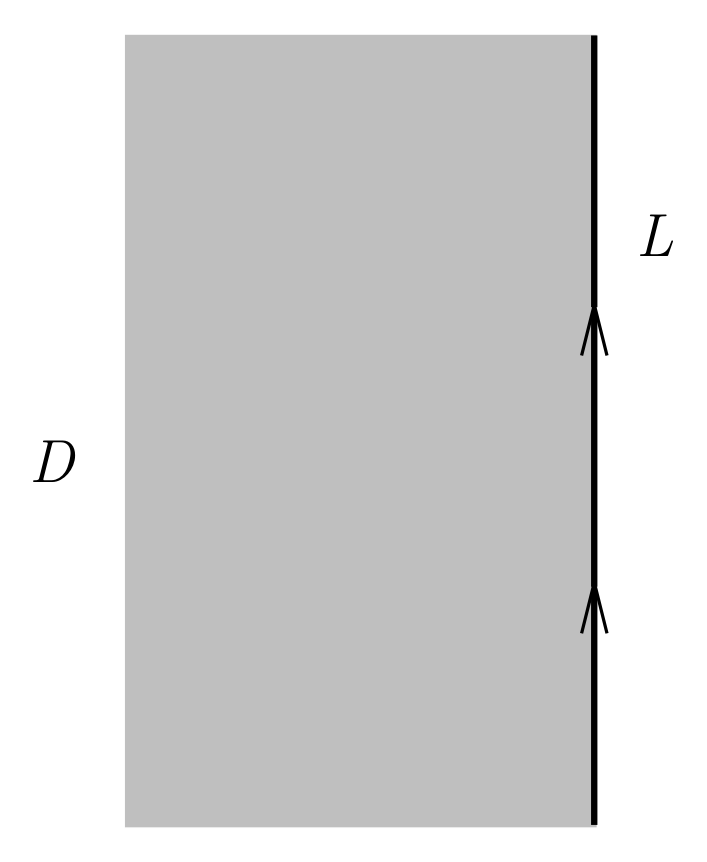
\includegraphics[width=0.62\linewidth]{figures/figure-1.png}
  \caption{一个面算符，其支撑 $D$ 带边界 $L$，而 $L$ 恰是磁单极子或双子的世界线。（原文 Fig.~1，PDF 第 25 页）}
  \label{fig:1}
\end{figure}

现在，把一些细节留给读者，并利用文献~\cite{ref14} 中的一些想法，
我们将对这一结果给出一个非正式的解读。

我们问：面算符的支撑 $D$ 能否像
图~\ref{fig:1} 那样带有边界 $L$？
稍加思考即可看出，若要如此，
$L$ 必须是磁荷为 $\alpha$ 的磁单极子（magnetic monopole）的世界线。绕 $D$ 的规范场和乐必须在边界
$L$ 处解绕，而和乐的这种解绕正是磁荷的特征。

然而，我们并未对磁荷 $\alpha$ 施加狄拉克量子化。既然
我们认为它是在模一个格向量的意义下定义的，那么真正关心的是
狄拉克量子化{\it 不}成立的情形。按照狄拉克的看法，此时为保持规范不变性，
$L$ 必须是通常所谓“狄拉克弦”（Dirac string）的世界体的边界。
在我们的语境中，曲面 $D$ 可以看作该弦的世界体。于是，
我们的面算符可以看作表示与量子化不正确的磁荷
相联系的狄拉克弦。狄拉克用绕弦的规范场单值性来定义狄拉克弦，
所以我们的面算符确实具备成为狄拉克弦世界体的正确性质。

更一般地，若 $\eta\not=0$，
弦末端的磁单极子还带有电荷，因此它是双子（dyon）。

我们关于 $(\alpha,\eta)$ 在 $S$-对偶下像磁荷与电荷一样变换的主张，
可以解读为：与量子化不正确的电荷相联系的狄拉克弦，
在对偶下的变换与正确量子化的电荷完全一样。

\begin{yizhu}[物理图像补充]把 $D$ 视为狄拉克弦世界体的图像与经典磁单极子构造完全平行（PDF 第 25--26 页）。对磁荷不满足
狄拉克量子化条件的磁单极子，必须从它引出一条奇异弦，使绕弦的规范场和乐失去定义；弦的位置并不物理，因为绕过弦一周矢势只差一个规范变换。
本文的面算符恰是把这条“人为”的奇异弦提升为物理算符：支撑 $D$ 就是弦的世界体，端点 $L$ 是磁单极子（或双子）的世界线。
这也说明为何 $\alpha$ 只在模格意义下有定义：把 $\alpha$ 改变一个格向量，只相当于改变丛的延拓，或让一条狄拉克弦穿过曲面。\end{yizhu}

最后给出一个相关的评论，文献~\cite{ref14} 中也有类似的预期。
从物理上说，若把 ${\mathcal N}=4$ 超杨–米尔斯理论
（或任何有兴趣的规范场论，例如标准模型）嵌入到某个在低能下约化为它的更完整的理论中，
面算符就可能出现。嵌入更完整的理论
可能产生在其他语境中所谓的宇宙弦（cosmic string）。假定这样的弦
足够重，以致可以认为它固定在某个位置，并在时空中有一条已知的轨道。
此时就适合考虑在弦存在下的“低能”${\mathcal N}=4$ 动力学。
这将涉及研究 ${\mathcal N}=4$ 理论与某种面算符的耦合。
细节取决于所考虑的具体宇宙弦类型。
产生 Aharonov–Bohm 效应的弦（最早在文献~\cite{ref10} 中探讨）会
导致本文所考虑的那类面算符。在第~\ref{sec:6.4}~节中，我们将考虑一些通过把 ${\mathcal N}=4$ 超杨–米尔斯理论嵌入
更完整的理论（更完整的理论为 IIB 型超弦理论）
而定义的面算符。在宇宙弦理论中，众所周知某些类型的弦可以
断裂，并终止于磁单极子上~\cite{ref47}。


\bigskip\noindent{\it 一个例证}

下面我们更详细地解释在
$G=SU(2)$、$^LG=SO(3)$ 的情形下 $S$-对偶如何作用在电荷上。这将使我们能够
说清楚前面分析中隐含的几点。
沿用文献~\cite{ref48}，我们解释两种不同的
看待该问题的方式。这一讨论在本文其余部分不会用到，
某些地方我们也讲得比较简略。

$SU(2)$ 是单连通的，所以对 $SU(2)$ 规范场论，
瞬子数取整数值，并且存在对称性
$T:\tau\to\tau+1$，其作用如式~\eqref{eq:2.50}。另一方面，对
$SO(3)$，瞬子数取值于 ${1\over 4}\mathbb{Z}$，
若 $M$ 是自旋流形则取值于 ${1\over 2}\mathbb{Z}$。所以 $\theta$ 角的基本
平移对称性是 $T^4:\tau\to\tau+4$，若 $M$ 自旋则为
$T^2:\tau\to\tau+2$。这些对称性的作用如
式~\eqref{eq:2.51}。此外还有对称性 $S:\tau\to -1/\tau$，
它交换 $SU(2)$ 与 $SO(3)$。当 $M$ 非自旋时，$SU(2)$ 规范场论的
对偶对称性群由下式生成：
% 式 (2.54)
\setcounter{equation}{53}
\begin{equation}\label{eq:2.54}
  T=\left(\begin{matrix}1&1\\ 0&1\end{matrix}\right),
~~~ST^4S^{-1}=\left(\begin{matrix}1&0\\-4&1\end{matrix}\right).
\end{equation}
（$ST^4S^{-1}$
是 $SU(2)$ 的对偶对称性，因为 $S^{-1}$ 把 $SU(2)$ 映到
$SO(3)$，$T^4$ 是 $SO(3)$ 的对偶变换，而 $S$
再映回 $SU(2)$。）这个对偶群称为
$\Gamma_0(4)$，是 $SL(2,\Z)$ 的同余子群（congruence subgroup）。它是
$SU(2)$ 规范场论在一般 $M$ 上的对偶对称性群，并且
按式~\eqref{eq:2.53} 作用在 $\alpha$ 与 $\eta$ 上。$SO(3)$ 规范场论的
对偶对称性群同样是 $\Gamma_0(4)$ 的一个拷贝，由 $STS^{-1}$ 与 $T^4$ 生成。
最后当然还有交换这两个群的对称性 $S$。若 $M$ 是自旋流形，则可处处把 4 换成 2，
对偶群同构于 $\Gamma_0(2)$。

$G=SU(2)$ 与 $^LG=SO(3)$ 具有相同的李代数，所以我们可以把
$\TT=\mathfrak t/\Lambda_{\rm rt}$ 与 $^L\neg\TT=\mathfrak t/\Lambda_{\rm wt}$ 看作
同一个空间按不同的格取的商，这两个格分别是
根格与权格（root and weight lattices）$\Lambda_{\rm rt}$ 与 $\Lambda_{\rm wt}$。
$\Lambda_{\rm rt}$ 在 $\Lambda_{\rm wt}$ 中的指数为二。
因此 $\mathfrak t$ 上的恒等映射
投影为从 $\TT$（$\alpha$ 的取值处）到
$^L\neg\TT$（$\eta$ 的取值处）的一个自然的二对一映射。
该映射隐含在变换 $T:(\alpha,\eta)\to
(\alpha,\eta+\alpha)$ 之中。$\mathfrak t$ 上的恒等映射
并不投影为 $^L\neg\TT\to\TT$ 的自然映射，但乘以 2（或任何偶数）的映射
却可以这样投影。于是存在一个自然映射 $ST^2S^{-1}:(\alpha,\eta)\to
(\alpha-2\eta,\eta)$，当 $M$ 是自旋流形时它实现为一个对偶
变换。类似地，运算
$ST^4S^{-1}:(\alpha,\eta)\to (\alpha-4\eta,\eta)$（它对任意 $M$ 都作为对偶变换出现）也是自然定义的。


这种描述方式与物理学文献的说法略有出入，因为那里对
诸如 $SU(2)$ 这样的单边群，对偶群一般被认为是
$SL(2,\Z)$。然而，通常的分析只对 $M=\R^4$ 进行，
且没有仔细考虑威尔逊算符与 't Hooft 算符。在这些
情形下，$SO(3)$ 与 $SU(2)$ 规范场论重合。
可以在 $\R^4$ 上通过添加二维表示中的威尔逊算符来区分这两种理论，以专门指
$SU(2)$；或者添加最小荷的 't Hooft 算符，以专门指
$SO(3)$。（不能同时添加这两类算符，
因为它们彼此不互局域。）如果按这种方式对 $SU(2)$ 与 $SO(3)$
理论加以细化，那么在 $\R^4$ 上合适的对偶群，恰恰就是
我们刚才在一般自旋流形上描述的那些。


其实，这个问题还有另一种表述，我们只给出其梗概，但它确实提供更多信息，
并且其中完整的群 $SL(2,\Z)$ 发挥作用。在这种
做法中，我们总把规范群取为伴随群
$SO(3)$（而不是它的覆盖群 $SU(2)$），但我们指定丛 $E$ 的
第二 Stieffel–Whitney 类 $\xi=w_2(E)$。对具有固定 $\xi$ 的所有 $SO(3)$-丛求和，我们为每个 $\xi$ 定义一个
配分函数\footnote{连同构成一个量子场论的一整套算符、关联函数、
量子态、膜等等。在更完整的描述中，被 $SL(2,\Z)$ 变换的是整个量子场论，
而不仅仅是这组配分函数。} $Z_\xi(\tau)$。然后可以证明
\cite{ref48}，$Z_\xi(\tau)$ 在一个 $SL(2,\Z)$ 的酉
表示中变换。

要把参数为 $\alpha,\eta$、支撑在曲面 $D$ 上的面算符
纳入这种做法，人们定义
$\alpha$ 与 $\eta$ 取值于 $\TT$，即单连通群 $SU(2)$ 的极大环面。于是对每个 $\xi$ 我们有一个
配分函数 $Z_\xi(\tau;\alpha,\eta)$，而主张是：
这一族配分函数按 $SL(2,\Z)$ 的一个表示变换（$SL(2,\Z)$ 以通常方式作用在 $\tau$ 上，
按文献~\cite{ref48} 所述作用在 $\xi$ 上，并按
式~\eqref{eq:2.53} 所述的自然作用，作用于 $\alpha$ 与
$\eta$ 上）。

用参数 $\xi,\alpha,\eta$ 来描述略有冗余。为说明这种
冗余，我们对极大环面 $\TT$（$\alpha$ 与 $\eta$ 的取值处）采用乘法记号，
并回忆这个环面含有 $SU(2)$ 中心的元素 $-1$。于是把 $\alpha$ 变为 $-\alpha$ 等价于按式~\eqref{eq:2.6} 把 $\xi$ 换成
$\xi+[D]$；而把 $\eta$ 变为 $-\eta$ 则使配分函数
$Z_\xi(\tau;\alpha,\eta)$ 乘以 $(-1)^{(\xi,D)}$（这一点在第~\ref{sec:4.2}~节末尾
有实质性的说明）。这种冗余与 $SL(2,\Z)$ 的作用相容，
但若不想让 $SL(2,\Z)$ 的作用显得更不自然，似乎很难把它消除。

\subsection{列维子群与更一般的面算符}

%% ==== 原文 §2.6：PDF 第 28 页（印刷第 27 页）====
\label{sec:2.6}

下面描述面算符定义的一个简单而重要的推广：把
极大环面 $\TT$ 换成 $G$ 的某个包含 $\TT$ 的更一般的子群 $\mathbb{L}$。
我们还假定 $\mathbb{L}$ 可以刻画为 $G$ 中与某个 $\alpha\in \mathfrak t$ 交换的子群。
这样的 $\mathbb{L}$ 称为 $G$ 的列维型子群（subgroup of Levi type）。
若两个这样的群在 $G$ 中共轭，就认为它们等价。
通常的情形是 $\alpha\not= 0$ 且 $\mathbb{L}$ 是 $G$ 的真子群，但我们也会
考虑 $\alpha=0$、$\mathbb{L}=G$ 的情形。任何列维子群（Levi subgroup）都包含 $\TT$，所以 $\TT$ 是极小列维子群。
非极小列维子群的一个典型例子是 $SU(3)$ 中如下形式的子群：

% 式 (2.55)
\setcounter{equation}{54}
\begin{equation}\label{eq:2.55}
  \left(\begin{matrix}* & * & 0 \\
                        * & * & 0 \\
                        0 & 0 & * \end{matrix}\right).
\end{equation}

它与 $U(2)$ 同构，实际上是一个次极小列维子群，因为
更小的列维子群只能是 $\TT$ 本身。一般地，对秩为 $r$ 的任意 $G$，
次极小列维子群同构于 $SU(2)\times U(1)^{r-1}$
或它对 $\Z_2$ 的商。

现在我们来定义所谓的 $\mathbb{L}$ 型面算符。按这种说法，
我们最初定义的面算符是 $\TT$ 型算符；我们也称它
为一般面算符。为定义 $\mathbb{L}$ 型面算符，我们考虑一个二维流形 $D$，其上带有
经典层面由通常参数 $(\alpha,\beta,\gamma)$ 标记的规范场论奇点。但
现在要求这些参数是 $\mathbb{L}$ 不变的。此外，当我们做量子
路径积分时，所除掉的规范变换是那些限制到 $D$ 上取值于 $\mathbb{L}$ 的变换，
而不只是取值于 $\TT$ 的那些。
正是由于最后这一步，$\mathbb{L}$ 型面算符才不只是我们最初
所定义的面算符（即 $(\alpha,\beta,
\gamma)$ 单纯取值于 $\mathfrak t$ 的 $\TT$ 型算符）在参数
为 $\mathbb{L}$ 不变时的特例。$\mathbb{L}$ 型面算符
是新东西，对应于不同的路径积分。事实上，我们将在第~\ref{sec:3.6}~节看到，若 $\mathbb{L}$ 以 $\TT$
为真子群，则当参数变为 $\mathbb{L}$ 不变时，$\TT$ 型面算符
会变得奇异。所以对于这类特殊参数，真正有意义的算符
是新的 $\mathbb{L}$ 型面算符。


在量子层面，还有一个额外的参数 $\eta$，即第~\ref{sec:2.3}~节的二维
$\theta$ 角 $\eta$。在当前情形下，群 $\TT$ 被 $\mathbb{L}$ 取代，
$\eta$ 不是取值于 $^L\neg \TT$，而是取值于某个子群。
事实上，我们希望把 $\eta$ 定义为 $\mathbb{L}$ 的阿贝尔部分的 $\theta$ 角。
为方便描述 $\eta$ 的取值，注意到列维子群 $\mathbb{L}\subset G$ 与
列维子群 $^L\neg \mathbb{L}\subset{} ^L\neg G$ 之间存在自然的对应。
描述这一对应的一种方式是：利用 $G$ 的外尔群 ${\mathcal W}$ 与
$^L\neg G$ 的外尔群 $^L\neg{\mathcal W}$ 自然等同这一事实。（见附录 A。）
此外，$\mathbb{L}$ 与 $^L\neg\mathbb{L}$
的外尔群分别是 ${\mathcal W}$ 与 $^L\neg {\mathcal W}$ 的子群。$\mathbb{L}$ 与 $^L\neg\mathbb{L}$ 之间的
对应简单说来就是它们有相同的外尔群，我们
把它记作 ${\mathcal W}_\mathbb{L}$。
表述 $\mathbb{L}$ 与 $^L\neg \mathbb{L}$ 之间对应的另一种说法是：$^L\neg \mathbb{L}$ 的余根
（它们是 $^L\neg G$ 的余根的子集）是 $\mathbb{L}$ 的余根的倍数——长余根与短余根
所乘的倍数不同。在明确了这些之后，
$\mathbb{L}$ 型面算符依赖于参数 $(\alpha,\beta,\gamma,\eta)$，它们
取值于 $\TT\times \mathfrak t\times \mathfrak t\times {}^L\neg
\TT$ 的 ${\mathcal W}_\mathbb{L}$ 不变部分。我们在这里用到了
如下事实：$(\alpha,\beta,\gamma)$ 的 $\mathbb{L}$ 不变性等价于
${\mathcal W}_\mathbb{L}$ 不变性。用 ${\mathcal W}_\mathbb{L}$ 不变性来表述有一个重要的
优点：它使我们能把 $\eta$ 与其他变量同等对待。
这比说 $(\alpha,\beta,\gamma)$ 是 $\mathbb{L}$ 不变的、
而 $\eta$ 是 $^L\neg \mathbb{L}$ 不变的要好。要求 $\eta$ 必须
为 ${\mathcal W}_\mathbb{L}$ 不变是正确的，因为这意味着 $\eta$ 是
限制在 $D$ 上的规范丛 $E$ 的阿贝尔磁通量的一个特征；
该丛的结构群是 $\mathbb{L}$，而它的特征类是
${\mathcal W}_\mathbb{L}$ 不变的。

我们把第~\ref{sec:2.4}~节的对偶猜想推广为：$\mathbb{L}$ 型面算符
在对偶下映为 $^L\neg \mathbb{L}$ 型面算符，参数
按熟悉的方式变换：$(\alpha,\beta,\gamma,\eta)\to(\eta,\beta,\gamma,-\alpha)$。


\bigskip\noindent{\it 更多群论}

下面描述一些在本文其余部分会用到的群论。

列维子群与所谓 $G_\C$ 的抛物子群密切相关。
取一个 $\alpha\in \mathfrak t$，使得与它交换的元素恰好组成 $\mathbb{L}$。我们说
这样的 $\alpha$ 是 $\mathbb{L}$-正则的（若 $\mathbb{L}=\TT$，就简单地说 $\alpha$ 是正则的）。
令 $\EUP$ 为 $G_\C$ 中李代数为 $\mathfrak p$ 的子群，
$\mathfrak p$ 由满足下式的元素 $\psi\in \mathfrak g$ 张成：
% 式 (2.56)
\setcounter{equation}{55}
\begin{equation}\label{eq:2.56}
  [\alpha,\psi]=i\lambda\psi,
~\lambda\geq 0.
\end{equation}
  这种形式的群称为 $G_\C$ 的抛物子群（parabolic subgroup）。
若在式~\eqref{eq:2.56} 中把条件 $\lambda\geq 0$ 换成 $\lambda>0$，我们便得到
子群 $\EUN\subset \EUP$ 的李代数
$\mathfrak n$，$\EUN$ 称为 $\EUP$ 的幂幺根（unipotent radical）。



例如，对 $G_\C=SL(3,\C)$ 与
$\mathbb{L}=\TT$，可以取 $\alpha=i\,{\rm diag}(y_1,y_2,y_3)$，其中 $y_i$ 为实数
且 $y_1>y_2>y_3$。此时得到的抛物群是上三角
矩阵构成的群

% 式 (2.57)
\setcounter{equation}{56}
\begin{equation}\label{eq:2.57}
  \left(\begin{matrix}*&*&*\\ 0&*&*\\ 0&0&*\end{matrix}\right),
\end{equation}

它称为博雷尔子群（Borel subgroup）$\EUB$。在这个例子中，幂幺根 $\EUN$
由如下形式的矩阵组成：

% 式 (2.58)
\setcounter{equation}{57}
\begin{equation}\label{eq:2.58}
  \left(\begin{matrix}1&*&*\\ 0&1&*\\ 0&0&1\end{matrix}\right),
\end{equation}


用外尔变换置换特征值，会得到另一个不同于我们所取的 $\TT$-正则（或简称正则）
$\alpha$。这导致一个外尔共轭的博雷尔
子群 $\EUB'$。
更一般地，对任意 $G$，
与序对 $(\TT,\alpha)$ 相联系的抛物子群
称为博雷尔子群 $\EUB$，它在外尔变换下唯一。
$\EUB$ 是极小抛物子群，正如 $\TT$ 是极小列维子群。

非极小列维子群 $\mathbb{L}$ 可能联系着若干个不等价的抛物子群。
例如，在式~\eqref{eq:2.55} 的例子中，我们可以取

% 式 (2.59)
\setcounter{equation}{58}
\begin{equation}\label{eq:2.59}
  \alpha=iy\left(\begin{matrix}1&0&0\\ 0&1&0\\ 0&0&-2\end{matrix}\right),
\end{equation}

其中 $y$ 为非零实数。若 $y$ 为正，得到由如下形式的矩阵
构成的抛物子群 $\EUP$：

% 式 (2.60)
\setcounter{equation}{59}
\begin{equation}\label{eq:2.60}
  \left(\begin{matrix}*& * & * \\
                        * & * & * \\
                        0 & 0 & * \end{matrix}\right),
\end{equation}
但若 $y$ 为负，则得到不等价的抛物子群 $\EUP'$，
                        它由如下形式的矩阵构成：

% 式 (2.61)
\setcounter{equation}{60}
\begin{equation}\label{eq:2.61}
  \left(\begin{matrix}* & * & 0 \\
                        * & * & 0\\
                        * & * & * \end{matrix}\right).
\end{equation}

幂幺根 $\EUN$ 与 $\EUN'$ 由如下形式的矩阵组成：

% 式 (2.62)
\setcounter{equation}{61}
\begin{equation}\label{eq:2.62}
  \left(\begin{matrix}1 & 0 & * \\
                        0 & 1 & * \\
                        0 & 0 & 1 \end{matrix}\right),
\end{equation}

或

% 式 (2.63)
\setcounter{equation}{62}
\begin{equation}\label{eq:2.63}
  \left(\begin{matrix}1 & 0 & 0 \\
                        0 & 1 & 0 \\
                        * & * & 1 \end{matrix}\right).
\end{equation}

\begin{yizhu}[易错点]式~\eqref{eq:2.59} 中 $\alpha$ 的正负给出\emph{不同}的抛物子群（PDF 第 30 页）：$\alpha$ 与 $-\alpha$ 分别对应彼此不共轭的
$\EUP$ 与 $\EUP'$（形状见式~\eqref{eq:2.60} 与式~\eqref{eq:2.61}），但两者的列维部分相同，都是式~\eqref{eq:2.55} 中的 $\mathbb{L}$。
所以“非极小列维子群联系着若干不等价的抛物子群”说的是：列维子群只固定块对角部分，而上三角或下三角的取向由 $\alpha$ 的指向（即 $(\TT,\alpha)$ 中的 $\alpha$）另行选定；
取 $\alpha=0$ 则退化为 $\mathbb{L}=G$、$\EUP=G_\C$ 的极大情形。\end{yizhu}

\bigskip\noindent{\it 极大列维子群}

若 $\alpha=0$，便得到上述构造的一个特殊情形：$\mathbb{L}=G$、$\EUP=G_\C$、
$\EUN=1$。最方便的做法是允许这一特殊情形，并把 $G$ 本身
看作一个极大列维子群。

在上面的讨论中，我们对 $\alpha$ 与 $\eta$ 是取值于李代数还是取值于环面
这一点略欠精确。取值于环面的情形给出更一般的构造，因为
${\mathcal W}_\mathbb{L}$ 不变的 $\alpha$ 或 $\eta$ 构成的空间可能不连通。我们针对
$\mathbb{L}=G$ 的情形把这一点说清楚。
$\alpha$ 为 $G$ 不变的条件表明它取值于 $G$ 的中心，我们
把它记作 ${\mathcal Z}(G)$。于是，支撑在曲面 $D$ 上的 $G$ 型面算符
的含义是：规范场定义在 $M\backslash D$ 上，
并且绕 $D$ 的单值性由指定的元素
$\alpha\in {\mathcal Z}(G)$ 标记。与选择 $\alpha$ 相对偶的是：
$D$ 上的 $G$-丛在拓扑上由一个特征类
$\xi\in H^2(D,\pi_1(G))\cong
\pi_1(G)$ 分类，而路径积分可以按取值于 ${\rm Hom}(\pi_1(G),U(1))$ 的离散 $\eta$ 角的选择
来加权。有限群 ${\mathcal Z}(G)$ 与 ${\rm Hom}(\pi_1(G),U(1))$ 在对偶下互换，
而自然的对偶猜想是：$\alpha$ 与 $\eta$ 的离散版本
按通常方式互换。

\begin{yizhu}[易错点]极大列维子群（$\mathbb{L}=G$，PDF 第 31 页）情形下，$\alpha$ 不再是李代数向量，而是中心里的离散元素
$\alpha\in{\mathcal Z}(G)$；$\eta$ 也变成取值于有限群 ${\rm Hom}(\pi_1(G),U(1))$ 的离散 $\theta$ 角。
原文指出，这两个有限群在对偶下互换，这正是式~\eqref{eq:2.25} 中 $S$ 交换 $\alpha,\eta$ 的离散版本。
注意不可把这一情形当作 §2.4--§2.5 环面取值情形的平凡极限：此处单值性取在中心里，反映的是 $G$-丛一般无法延拓过 $D$，
其障碍正是特征类 $\xi\in H^2(D,\pi_1(G))$。\end{yizhu}

虽然我们关于 $\mathbb{L}$ 型面算符的对偶猜想意在
涵盖这些不连通分支，本文不会详细
讨论它们。


%% ============================================================
%% 片段：s03a-quotient   对应原文 PDF 第 32--47 页
%% 本文件由 gw/convert.py 从 arXiv 源码（hep-th/0612073v2）自动生成：
%%   * 公式/编号/引用/图 已经锁定为原文内容，请勿改动任何数学内容与编号；
%%   * 只需把英文正文译为中文，并在每节开头加“本节重点”、关键处加译注。
%% ============================================================


\section{经典几何续论}

%% ==== 原文 §3：PDF 第 32 页（印刷第 31 页）====
\label{sec:3}

\begin{keytakeaways}
  \begin{itemize}[leftmargin=1.4em,itemsep=2pt,topsep=2pt]
    \item \textbf{物理图像}：带分歧的希格斯丛模空间 $\MH(\alpha,\beta,\gamma;p)$ 是超 Kähler 商 $\EUW(\alpha,\beta,\gamma;p)/\neg/\neg/\EUG_p$；参数 $(\alpha,\beta,\gamma)\in\mathfrak t\times\mathfrak t\times\mathfrak t$ 刻画面算符在分歧点 $p$ 处的奇异类型，而面算符所对应的量子场论问题由列维子群 $\mathbb{L}$ 的选择决定。
    \item \textbf{数学工具}：超 Kähler 矩映射 $\vec\mu=(\mu_I,\mu_J,\mu_K)$ 与三个 Kähler 形式 $\omega_I,\omega_J,\omega_K$；复观点在适当的稳定性条件下把超 Kähler 商等同于几何不变量理论商 $\nu_I^{-1}(0)/\EUG_{p,\C}$，从而与稳定抛物希格斯丛（复结构 $I$）或稳定抛物局部系统（复结构 $J$）的模空间联系起来。
    \item \textbf{关键结论}：三个 Kähler 形式的上同调类都是 $(\alpha,\beta,\gamma)$ 的线性函数，即式~\eqref{eq:3.8}--\eqref{eq:3.10}；并且只要避开实余维至少为二的奇点，实辛簇 $(\MH,\omega_K)$ 就与 $\alpha$、$\beta$ 无关。
    \item \textbf{非正则情形}：$(\alpha,\gamma)$ 或 $(\beta,\gamma)$ 非正则时，单值性只能确定到共轭类的闭包中：半单部分由 $U=\exp(-2\pi(\alpha-i\gamma))$ 给出，幂幺部分落在由 $\beta$ 决定的幂幺根 $\EUN$ 内，一般情形下落在理查森类中；相应的局部解由纳姆方程（Nahm's equations）描述（脚注~17、第~\ref{sec:3.8}~节）。
  \end{itemize}
\end{keytakeaways}

本节将重新考察第~\ref{sec:2.2}~节的构造，并描述那些需要更深入地理解 $\MH$ 的经典几何才能说明的方面。我们力求给出一个相对简单——但当然并不数学上完整——的介绍，涵盖那些目前或可能对几何朗兰兹纲领有用的内容。我们所讨论的大部分课题在数学文献中已有远为充分的处理，但有几处也许是新的，特别是仿射外尔群（affine Weyl group）在 $\MH$ 的上同调（cohomology）上的作用（第~\ref{sec:3.7}~节）、辛形式的上同调类的线性性（第~\ref{sec:3.2}~节），以及 $\MH$ 在非正则点处局部奇点的性质（第~\ref{sec:3.6}~节）。

我们将描述的许多最重要现象都有局部模型，这些模型涉及复余伴随轨道（complex coadjoint orbit）上的超 Kähler（hyper-Kähler）度规，其构造见 \cite{ref34,ref35,ref36,ref37}。我们把这部分推迟到第~\ref{sec:3.8}~节。



\subsection{超 Kähler 商}
 %% ==== 原文 §3.1：PDF 第 32 页（印刷第 31 页）====
\label{sec:3.1}

黎曼面 $C$ 上希格斯丛（Higgs bundle）的模空间（moduli space）$\MH(G,C)$ 的最基本性质之一是，它可以构造为超 Kähler 商（hyper-Kähler quotient）\cite{ref21}。我们首先回顾无奇点时的构造。取光滑的 $G$-丛 $E\to C$，以 $\EUW$ 记数对 $(A,\phi)$ 构成的空间，其中 $A$ 是 $E$ 上的联络（connection），$\phi\in
\Omega^1(C,{\rm ad}(E))$。$\EUW$ 是平坦的超 Kähler 流形；详细论述见 \cite{ref8} 第 4.1 节。设 $\EUG$ 是 $E$ 的规范变换（gauge transformation）群。则 $\EUG$ 作用在 $\EUW$ 上，保持超 Kähler 结构，并带有超 Kähler 矩映射（moment map）$\vec\mu=(\mu_I,\mu_J,\mu_K)$：

% 式 (3.1)
\setcounter{equation}{0}
\begin{equation}\label{eq:3.1}
  \begin{aligned}\mu_I & =-{1\over
2\pi}\int_C\,\Tr\,\epsilon(F-\phi\wedge \phi),\\ \mu_J &
=-{1\over 2\pi}\int_C|d^2z|\,\Tr\,\epsilon\left(D_z\phi_{\bar
z}+D_{\bar z}\phi_z\right), \\ \mu_K& = -{i\over
2\pi}\int_C|d^2z|\,\Tr\,\epsilon\left(D_z\phi_{\bar z}-D_{\bar
z}\phi_z\right).\end{aligned}
\end{equation}
这里 $\epsilon\in \Omega^0(C,{\rm ad}(E))$
是 $\EUG$ 的李代数的一个元素；$\vec\mu$ 关于 $\epsilon$ 是线性的。给定超 Kähler 流形 $\EUW$ 以及保持超 Kähler 结构、作用在 $\EUW$ 上并带有矩映射 $\vec\mu$ 的群
$\EUG$，超 Kähler 商
$\EUW/\neg/\neg/\EUG$ 一般地 \cite{ref49} 定义为 $\vec\mu^{-1}(0)/\EUG$。该超 Kähler 商是超 Kähler 流形。在目前的情形下，方程
$\vec\mu=0$（对所有 $\epsilon$）正是希钦方程（Hitchin's equations）\eqref{eq:2.1}。于是超 Kähler 商 $\EUW/\neg/\neg/\EUG$ 恰好是希钦方程之解的模空间 $\MH$。

\begin{yizhu}[易错点]
这里的除法应理解为几何不变量理论意义下的商，而非集合论意义上的商：$\EUG$ 在 $\vec\mu^{-1}(0)$ 上的作用一般有非平凡稳定子，商空间因此会出现轨形（orbifold）奇点。第~\ref{sec:3.2}~节把同一对象改写成复结构 $I$ 下的 GIT 商 $\nu_I^{-1}(0)/\EUG_{p,\C}$ 时，这一点表现得最清楚。GIT 商的稳定性条件一般依赖于 $\alpha$（当 $\sigma$ 一般时与 $\alpha$ 无关，见第~\ref{sec:3.2}~节），所以“超 Kähler 商 $=$ 辛商 $=$ GIT 商”这一串等同并非对任意参数都自动成立；跨墙（wall-crossing）现象正是稳定性条件改变时发生的。另注意 $\MH$ 只通过 $\alpha$ 在 $\mathfrak t/\Lambda_{\cochar}=\TT$ 中的像依赖于 $\alpha$（脚注~14）。
\end{yizhu}

这一构造可以推广到带有熟知类型孤立奇点的希格斯丛 \cite{ref23,ref24}。取一点 $p\in C$，并把丛 $E$ 在 $p $ 处的结构群约化为环面 $\TT$，以 $\EUG_p$ 记 $\EUG$ 中在 $p$ 处的限制落在 $\TT$ 内的规范变换构成的子群。再取三元组\footnote{正如第~\ref{sec:2.1}~节所解释的，$\MH$ 实际上只依赖于 $\alpha$ 在 $\mathfrak t/\Lambda_{\cochar}=\TT$ 中的像。}
$(\alpha,\beta,\gamma)\in \mathfrak t$（$\TT$ 的李代数）。在 $p$ 附近取坐标 $r,\theta$，以 $\EUW(\alpha,\beta,\gamma;p)$ 记在 $p$ 附近具有熟知类型奇点的数对 $(A,\phi)$ 构成的空间：

% 式 (3.2)
\setcounter{equation}{1}
\begin{equation}\label{eq:3.2}
  \begin{aligned}A & =\alpha\,d\theta+\dots\\
 \phi & = \beta\,{dr\over r}-\gamma\,d\theta+\dots.\end{aligned}
\end{equation}

省略号表示比 $1/r$ 更不奇异的项。又记 $\EUG_p$ 为 $E$ 的规范变换中在 $p$ 处取值于 $\TT$ 的群。这些正是保持条件~\eqref{eq:3.2} 不变的规范变换。于是模空间 $\M_H(\alpha,\beta,\gamma;p)$ 就是超 Kähler 商
$\EUW(\alpha,\beta,\gamma;p)/\neg/\neg/\EUG_p$。我们称之为在点 $p$ 处带分歧的希格斯丛的模空间。类似地，可以把在若干点处带分歧的希格斯丛的相应模空间也构造为超 Kähler 商，即在若干点 $p_1,\dots,p_s\in C$ 处具有奇点、并由参数 $(\alpha_i,\beta_i,\gamma_i)\in \mathfrak t$（$i=1,\dots,s$）标记的希钦方程之解的模空间。为记号简洁起见，本节主要就单点分歧的情形陈述，但所有论断对更一般的情形都有直接类比。

具有复结构（complex structure）$I,J,$ 和 $K$ 的超 Kähler 流形，具有相应的 Kähler 形式 $\omega_I$、$\omega_J$ 和
$\omega_K$。在目前的情形下，这些形式可以像无奇点时那样写出，\footnote{与 \cite{ref8} 一样，我们以 $\delta$ 记 $\EUW$ 上的外微分，以 $d$ 记 $C$ 上的外微分。}
% 式 (3.3)
\setcounter{equation}{2}
\begin{equation}\label{eq:3.3}
  \begin{aligned}\omega_I & =
-{i\over 2\pi}\int_C|d^2z|\,\Tr\left(\delta A_{\bar z}\wedge
\delta A_z-\delta \phi_{\bar z}\wedge \delta\phi_z\right)\\
&=-{1\over 4\pi}\int_C\,\Tr\left(\delta A\wedge \delta A
-\delta\phi\wedge\delta \phi\right) \\
                      \omega_J & ={1\over 2\pi}\int_C |d^2z|\,\Tr\left(
                      \delta\phi_{\bar z}\wedge \delta A_z+\delta\phi_z\wedge
                      \delta A_{\bar z} \right)\\
                      \omega_K & =
                      {i\over 2\pi}\int_C|d^2z|\,\Tr\left(\delta\phi_{\bar z}
                      \wedge\delta A_z-\delta\phi_z\wedge\delta A_{\bar z}\right)\\
                      & = {1\over 2\pi}\int_C \,\Tr\,\delta\phi
                      \wedge\delta A.\end{aligned}
\end{equation}


正如无奇点时那样（见 \cite{ref8} 第 4.1 节），$\omega_I$ 与
% 式 (3.4)
\setcounter{equation}{3}
\begin{equation}\label{eq:3.4}
  \omega_I'  =
-{i\over 2\pi}\int_C|d^2z|\,\Tr\left(\delta A_{\bar z}\wedge
\delta A_z\right)=-{1\over 4\pi}\int_C\,\Tr\left(\delta A\wedge
\delta A \right),
\end{equation}
上同调，后者只依赖于 $A$，因而来自 $G$-丛的模空间 $\M$ 的拉回。事实上，令 $\lambda_I={1\over 4\pi}\int_C\Tr
\,\phi\wedge\delta \phi$。$\lambda_I$ 是规范不变的，且（在分部积分并使用希钦方程之后）与规范变换的生成元 $\delta A=-d_A\epsilon,
\,\delta\phi=[\epsilon,\phi]$ 缩并时为零。因此它是 $\MH$ 上某个一形式的拉回，而公式
$\omega_I-\omega_I'=\delta\lambda_I$ 表明 $\omega_I$ 与 $\omega_I'$ 上同调等价。

\begin{yizhu}[易错点]
超 Kähler 流形的三个复结构 $I,J,K$ 与三个 Kähler 形式 $\omega_I,\omega_J,\omega_K$ 一一对应（约定 $\omega_I(\cdot,\cdot)=g(I\cdot,\cdot)$ 等），而三个全纯辛形式是 $\Omega_I=\omega_J+i\omega_K$、$\Omega_J=\omega_K+i\omega_I$、$\Omega_K=\omega_I+i\omega_J$。核对本节结论时须注意指标并不“对齐”：式~\eqref{eq:3.8} 说 $[\,\omega_I]$ 只依赖 $\alpha$，而第~\ref{sec:3.2}~节说 $\Omega_I=\omega_J+i\omega_K$ 的全纯参数是 $\beta+i\gamma$；类似地 $\Omega_J$ 依赖 $\gamma+i\alpha$、$\Omega_K$ 依赖 $\alpha+i\beta$。把这两组对应关系混同是本节最常见的错误来源。
\end{yizhu}

无奇点时，$\omega_J$ 与 $\omega_K$ 的上同调类为零。例如，对 $\omega_K$ 可以写出 $\omega_K=\delta\lambda_K$（其中 $\lambda_K={1\over 2\pi}\int_C\Tr \,\phi\wedge\delta A$）来证明这一点。只要 $\gamma=0$，这在存在奇点时仍然成立；但当 $\gamma\not=0$ 时，$\lambda_K$ 与规范变换的生成元缩并后不为零，因而它不是 $\MH$ 上一形式的拉回。事实上，与规范变换的生成元缩并把 $\omega_K$ 映为 ${1\over
2\pi}\int_C\Tr\,\phi\wedge (-d_A\epsilon)= \Tr\,\gamma \epsilon(p)$，这里我们用了分部积分以及 $d_A\phi=-2\pi \gamma \delta_p$。所以当 $\gamma\not=0$ 时 $\omega_K$ 的上同调类非零。类似地，当 $\beta\not=0$ 时 $\omega_J$ 的上同调类非零。我们将在第~\ref{sec:3.6}~节描述所有这些上同调类。

\bigskip\noindent{\it $\mathbb{L}$ 型的推广}

我们可以容易地把这一点推广到包含一般列维子群 $\mathbb{L}$ 的情形。

我们把参数 $(\alpha,\beta,\gamma)$ 限制为 $\mathbb{L}$-不变的。把 $\EUG_p$ 定义为在 $p$ 处的限制落在 $\mathbb{L}$ 中（而非如上文那样落在 $\TT$ 中）的规范变换群。完全照上面进行，超 Kähler 商 $\EUW(\alpha,\beta,\gamma;p)/\neg/\neg/\EUG_p$
现在给出我们将称为 $\M_{H,\mathbb{L}}$ 的对象，即具有 $\mathbb{L}$ 型分歧结构的希格斯丛的模空间。严格的构造见 \cite{ref23}。当我们不明确指出分歧型时，就意味着取 $\mathbb{L}=\TT$。

在定义 $\M_{H,\mathbb{L}}$ 时必须小心，要求解偏离由 $(\alpha,\beta,\gamma)$ 决定的渐近形式的项比 $1/r\ln r$ 更小，而不仅仅是比 $1/r$ 更小。这样做的目的是排除下文式~\eqref{eq:3.101} 所示的那种渐近行为。

我们之所以为 $\M_{H,\mathbb{L}}(\alpha,\beta,\gamma;p)$ 引入特殊记号，是因为（希望在第~\ref{sec:3.6}~节会变得清楚）它并不是 $\M_H(\alpha,\beta,\gamma;p)$（对正则三元组 $(\alpha,\beta,\gamma)$ 定义）在 $(\alpha,\beta,\gamma)$ 趋于 $\mathbb{L}$-不变值时的极限。这两个空间连维数都不相同。它们的关系是：当三元组 $(\alpha,\beta,\gamma)$ 变为 $\mathbb{L}$-不变时，$\M_{H,\mathbb{L}}$ 是 $\MH$ 的一个奇点轨迹。

本定义的一个特例是 $\mathbb{L}=G$。$G$ 型的分歧结构可以根本没有分歧，因为在 $p$ 处取值于 $G$ 的规范变换群就是全体规范变换。不过，正如第~\ref{sec:2.6}~节末尾所讨论的，若 $G$ 有非平凡的中心 ${\mathcal Z}$，我们的定义有一个轻微的推广。确实，三元组 $(\alpha,\beta,\gamma)
\in \TT\times \mathfrak t\times \mathfrak t$ 是 $G$-不变的，当且仅当 $\beta=\gamma=0$ 且 $\alpha$ 是 ${\mathcal Z}$ 的一个元素。于是 $\M_{H,G}$ 是由 ${\mathcal Z}$ 标记的若干分支之并。其中一个分支（对应 $\mathcal Z$ 的单位元）就是通常的、在 $p$ 处无奇点的希格斯丛的模空间 $\MH$。

另一个极端是 $\mathbb{L}=\TT$。此时 $\M_{H,\mathbb{L}}(\alpha,\beta,\gamma;p)$ 就是我们通常简记为 $\M_H(\alpha,\beta,\gamma;p)$ 的对象。当我们不指定 $\mathbb{L}$ 而谈论带分歧的希格斯丛时，所指的就是这个一般情形。

我们的观点是：支撑在曲面 $D$ 上的面算符（surface operator）由列维型群 $\mathbb{L}$ 的选择来定义。一个特定的面算符导致一个特定的量子场论问题，以及一个特定的带分歧希格斯丛的模空间 $\M_{H,\mathbb{L}}$。在 $\M_{H,\mathbb{L}}$ 的理论中，有时会强调抛物结构（parabolic structure），这一概念我们将在第~\ref{sec:3.4}~节解释。正如我们将看到的（也可以从第~\ref{sec:2.6}~节抛物子群的定义预计到），用抛物结构所作的诠释依赖于 $\alpha$ 取 $\mathbb{L}$-正则值。文献 \cite{ref24} 指出，在保持 $\mathbb{L}$ 固定不变的情况下，通过同时改变 $\beta$、$\gamma$ 和 $\alpha$，可以不遇到奇点而从一种抛物型过渡到另一种抛物型。因此同一个面算符可以导致不同种类的抛物结构；与其按抛物型，不如按列维型来标记面算符。这就是为什么我们宁愿说带分歧的希格斯丛的模空间，而不说抛物希格斯丛（parabolic Higgs bundle）的模空间。不过，当强调复结构 $I$ 的作用时，我们仍会说抛物希格斯丛，因为在那里这一术语是标准的。

\subsection{复观点}
 %% ==== 原文 §3.2：PDF 第 36 页（印刷第 35 页）====
\label{sec:3.2}

人们常常可以通过聚焦于其中一个复结构（例如 $I$）来更多地了解超 Kähler 商 \cite{ref49}。函数
 $\nu_I=\mu_J+i\mu_K$ 在复结构 $I$ 下全纯（holomorphic）。超 Kähler 商 $\EUW/\neg/\neg/\EUG_p$ 等同于用 $\EUG_p$ 对 $\nu_I^{-1}(0)$ 作辛商（symplectic quotient）。（该辛商的定义是：把限制在 $\nu_I^{-1}(0)$ 上的通常矩映射
$\mu_I$ 置零，然后除以 $\EUG_p$。此时 $\nu_I$ 与 $\mu_I$ 都已置零，正给出超 Kähler 商。）按照辛商与复解析商（complex analytic quotient）之间的通常关系，用 $\EUG_p$ 对 $\nu_I^{-1}(0)$ 作辛商，也可以作为几何不变量理论商 $\nu_I^{-1}(0)/\EUG_{p,\C}$ 得到，其中 $\EUG_{p,\C}$ 是 $\EUG_p$ 的复化（complexification）。（由于
$\EUW$ 是带有 $\EUG_p$ 线性作用的仿射空间，一旦选定 $\EUW$ 的某个复结构，$\EUG_p$ 的复化 $\EUG_{p,\C}$ 就自然地作用在 $\EUW$ 上。）若把复结构 $I$ 换成构成 $\EUW$ 超 Kähler 结构的任一复结构，所有这些陈述都有类比。

在目前的情形下，$\nu_I^{-1}(0)/\EUG_{p,\C}$ 可以有全纯的描述，即作为稳定抛物希格斯丛 $(E,\varphi)$ 的模空间。这一点在 \cite{ref22,ref23} 中有解释。就我们的目的而言，并不真正需要这些细节，但确实需要这样一个描述存在这一事实。粗略地说，在指定点 $p\in C$ 处带抛物结构的抛物希格斯丛，是一个希格斯丛
$(E,\varphi)$，其中 $E$ 是 $C$ 上的全纯 $G_\C$-丛，$\varphi$
是 $K_C\otimes {\rm ad}(E)$ 的一个截面，在 $p$ 之外全纯，并在 $p$ 处有一个满足某条件的单极点（simple pole）。若 $\sigma=\half(\beta+i\gamma)$ 是正则的，即它恰好与 $\TT$（更一般地，与 $\mathbb{L}$）交换，则该条件可从式~\eqref{eq:2.11}\ 预计到：$\varphi$ 的极点部分共轭于 $\sigma\,dz/z$。（这里 $z$ 是 $p$ 附近的局部全纯参数。）若 $\sigma$ 不正则，会发生什么则推迟到第~\ref{sec:3.3}~节解释。

抛物希格斯丛的稳定（stable）条件一般依赖于 $\alpha$，但若 $\sigma$ 是一般的，则与 $\alpha$ 无关 \cite{ref24}。在 Kähler 几何中，人们会预期在 $\alpha$ 的特殊值处出现跨墙现象，但在超 Kähler 几何中，对一般的 $\sigma$ 这一现象被回避，正如我们在第~\ref{sec:3.6}~节所解释的。

稳定抛物希格斯丛的模空间（我们暂时记作 $\tilde\M_H$）是复辛流形，带有全纯辛形式（holomorphic symplectic form）$\Omega_I=\omega_J+i\omega_K$。此外，$\tilde\M_H$ 的复结构以及 $\Omega_I$ 的上同调类明显地关于 $\beta+i\gamma$ 全纯。若 $\sigma$ 是一般的，它们也明显地与 $\alpha$ 无关（因为 $\alpha$ 只影响稳定性条件）。

由于把 $\MH(\alpha,\beta,\gamma;p)$ 视为复结构 $I$ 下的复流形时与 $\tilde\M_H$ 相同，所有这些陈述对 $\MH(\alpha,\beta,\gamma;p)$ 都有直接的推论。它们解释了第~\ref{sec:2.2}~节表格中所作的某些论断。特别地，$\MH$ 上的复结构 $I$ 关于 $\beta+i\gamma$ 全纯地变化，且与 $\alpha$ 无关。此外，若以 $[\,\omega]$ 记闭微分形式 $\omega$ 的上同调类，则上同调类 $[\Omega_I]$ 关于 $\beta+i\gamma$ 全纯地变化，且与 $\alpha$ 无关。特别地，类 $[\,\omega_J]$ 与 $[\,\omega_K]$ 与 $\alpha$ 无关。

\bigskip\noindent{\it 其他复结构中的类比}

当然，在复结构 $J$ 中有类似的故事。商 $\nu_J^{-1}(0)/\EUG_{p,\C}$ 可以有全纯的解释，即作为稳定抛物（或带滤过的）局部系统（parabolic (or filtered) local system）的模空间。抛物局部系统是 $C\backslash p$（即去掉点 $p$ 的 $C$）上取值于 $G_{\C}$ 的平坦联络，并带有对绕 $p$ 的单值性的约束。我们把这个单值性记作 $V$。若 $G_\C$ 中的元素 $U=\exp(-2\pi(\alpha-i\gamma))$ 是正则的（意思是与它交换的 $G_\C$ 的子群恰好是环面 $\TT$），则对单值性的约束是 $V$ 必须共轭于 $U$，正如我们从式~\eqref{eq:2.12} 所预期的。否则就需要更精细的描述，我们将它推迟到第~\ref{sec:3.3}~节。抛物局部系统的稳定条件一般依赖于 $\beta$，但若 $\gamma+i\alpha$ 是一般的，则与 $\beta$ 无关 \cite{ref24}。

稳定抛物局部系统的模空间 $\hat \M_H$ 是复辛流形，带有全纯辛形式
$\Omega_J=\omega_K+i\omega_I$。现在我们作与复结构 $I$ 中相同的论证。$\MH$ 视为复结构 $J$ 下的复流形时与 $\hat \M_H$ 相同这一事实，使第~\ref{sec:2.2}~节表格中所作的某些论断变得显然。特别地，$\MH$ 上的复结构 $J$ 关于 $\gamma+i\alpha$ 全纯地变化，且与 $\beta$ 无关。类似地，上同调类 $[\Omega_J]$ 关于 $\gamma+i\alpha$ 全纯，且与 $\beta$ 无关。因此 $[\,\omega_K]$ 与 $[\,\omega_I]$ 与 $\beta$ 无关。


当然，我们可以在复结构 $K$ 中作同样的推理，以证明 $\MH$ 的复结构 $K$ 与辛结构 $\Omega_K$ 关于 $\alpha+i\beta$ 全纯且与 $\gamma$ 无关。于是特别地，上同调类 $[\,\omega_I]$ 与 $[\,\omega_J]$ 与 $\gamma$ 无关。至此完成了对第~\ref{sec:2.2}~节表格中诸论断的论证。




\bigskip\noindent{\it 上同调类的线性性}

利用同样的推理适用于构成 $\MH$ 超 Kähler 结构的任一复结构这一事实，我们可以走得更远。这样的复结构具有形式 $\hat I=pI+qJ+rK$，其中实参数 $p,q,$ 和 $r$ 满足
$p^2+q^2+r^2=1$。第~\ref{sec:2.2}~节表格中的所有论断对任一 $\hat I$ 都有类比。确实，若我们对由复结构 $I,J,K$ 张成的空间作一个 $SO(3)$ 旋转，同时对由三个辛结构 $\omega_I$、$\omega_J$ 和 $\omega_K$ 张成的空间以及由三个变量 $\alpha,$ $\beta$ 和 $\gamma$ 张成的空间作同样的旋转，这些论断仍然成立。这个 $SO(3)$ 不是 $\MH$ 的对称性，但它是我们推导表格中论断所用推理的对称性。

这使我们能对上同调类 $[\,\omega_I]$、$[\,\omega_J]$ 和 $[\,\omega_K]$ 作出一些简单的推断。把这些上同调类记作 $x_i$，$i=1,2,3$。于是 $x_i$ 取值于向量空间
$H^2(\MH,\R)$。它们是 $\alpha,\beta$ 和 $\gamma$ 的函数，我们把这些变量记作 $y_i$，$i=1,2,3$。那么迄今为止所确立的是
% 式 (3.5)
\setcounter{equation}{4}
\begin{equation}\label{eq:3.5}
  {\partial x_i\over\partial
y_j}=0,~~i\not= j.
\end{equation}
然而，通过在一般的复结构 $\hat I$ 中作同样的论证，我们得知：对 $\vec
x=(x_1,x_2,x_3)$ 与 $\vec y=(y_1,y_2,y_3)$ 作一个 $SO(3)$ 旋转后，\eqref{eq:3.5}\ 仍然成立。这意味着
% 式 (3.6)
\setcounter{equation}{5}
\begin{equation}\label{eq:3.6}
  {\partial x_i\over\partial y_j}=\delta_{ij}v
\end{equation}
对
某函数 $v$ 成立（它取值于 $H^2(\MH,\R)$）。\footnote{
这等价于如下陈述：对任意复结构 $\hat I=pI+qJ+rK$，相应的全纯 $(2,0)$ 形式 $\Omega_{\hat I}$（由
$\Omega_I$ 经适当的
$SO(3)$ 旋转得到）的上同调类与 Kähler 形式（它是
$p\alpha+q\beta+r\gamma$ 的倍数）无关。} 再求导一次，由式~\eqref{eq:3.6} 得到
% 式 (3.7)
\setcounter{equation}{6}
\begin{equation}\label{eq:3.7}
  \delta_{ij}{\partial
v\over \partial x_k}=\delta_{ik}{\partial v\over\partial x_j}.
\end{equation}

但这蕴含着（考虑 $i=j$、$i\not= k$ 的情形）对一切 $k$ 有 $\partial v/\partial x_k=0$，故
$v$ 是常数。

\begin{yizhu}[含糊点拨]
由式~\eqref{eq:3.6} 得到~\eqref{eq:3.7} 这一步，原文只说“再求导一次”，其实隐含了链式法则：对 (3.6) 关于 $y_k$ 求导给出 $\partial^2x_i/\partial y_j\partial y_k=\delta_{ij}\partial v/\partial y_k$，由混合偏导的对称性得 $\delta_{ij}\partial v/\partial y_k=\delta_{ik}\partial v/\partial y_j$；再借 $\partial x_i/\partial y_j=\delta_{ij}v$（即 $\partial/\partial y_k=v\,\partial/\partial x_k$，要求 $v\not=0$）把 $\partial v/\partial y$ 换成 $\partial v/\partial x$，方得 (3.7)。因此 $x$ 与 $y$ 之间变换的可逆性与 $v\not=0$ 是隐含前提；若某个参数值上 $v=0$，需用连续性延拓过去。
\end{yizhu}

既然 $v$ 是常数，\eqref{eq:3.6} 就表明 $x_i$ 是 $y_j$ 的线性函数。特别地，$[\,\omega_I]$——我们已知它只依赖于 $\alpha$——实际上是 $\alpha$ 的{\it 线性}函数。于是
% 式 (3.8)
\setcounter{equation}{7}
\begin{equation}\label{eq:3.8}
  [\,\omega_I]=a+\Tr\,\alpha h
\end{equation}
其中 $a$、$h$ 为某些常数。（$a$ 取值于
$H^2(\MH,\R)$，$h$ 取值于 $H^2(\MH,\R)\otimes {\mathfrak t}$。）类似地，我们已经知道 $[\,\omega_J]$ 只依赖于 $\beta$
且在 $\beta=0$ 时为零；现在可由 \eqref{eq:3.6} 推出
% 式 (3.9)
\setcounter{equation}{8}
\begin{equation}\label{eq:3.9}
  [\,\omega_J]=\Tr\,\beta h
\end{equation}
其中 $h$ 与 \eqref{eq:3.8} 中的相同。同理，
% 式 (3.10)
\setcounter{equation}{9}
\begin{equation}\label{eq:3.10}
  [\,\omega_K]=\Tr\,\gamma h.
\end{equation}
我们将在第~\ref{sec:3.5}~节和第~\ref{sec:3.6}~节描述 $a$ 与 $h$。

\bigskip\noindent{\it $\MH$ 作为辛簇}

  正如我们刚才所见，上同调类 $[\,\omega_K]$ 与 $\alpha$ 和 $\beta$ 无关。若 $\MH$ 是紧的，由此便可得：以 $\omega_K$ 为辛结构的实辛簇（real symplectic variety）$\MH$ 与 $\alpha$、$\beta$ 无关。由于 $\MH$ 非紧，这一结论不能仅由辛形式上同调类的常性推出；但更仔细地考察我们用来证明该常性的事实，就可以得到它。

为了在改变 $\alpha$ 时不改变实辛簇 $(\MH,\omega_K)$，我们只需把 $\MH$ 放在复结构 $I$ 中看。由于有抛物希格斯丛的解释，这个复结构以及相应的全纯二形式
$\Omega_I=\omega_J+i\omega_K$ 与 $\alpha$ 无关，只要避开某些奇点。于是我们可以在保持实辛簇
$(\MH,\omega_K)$ 不变的情况下改变 $\alpha$。

类似地，为了在改变 $\beta$ 时不改变实辛簇 $(\MH,\omega_K)$，我们只需把 $\MH$ 放在复结构
$J$ 中看。由于有带滤过局部系统的解释，这个复结构以及相应的全纯二形式
$\Omega_J=\omega_K+i\omega_I$ 与 $\beta$ 无关，只要避开某些奇点。于是我们可以在保持实辛簇
$(\MH,\omega_K)$ 不变的情况下改变 $\beta$。

此过程中必须避开的奇点在第~\ref{sec:3.6}~节中描述，其实余维（codimension）至少为二。于是我们断言：实辛簇 $(\MH,\omega_K)$ 与 $\alpha$ 和 $\beta$ 无关——这是应用于几何朗兰兹纲领的一个重要结果。

一个要点是：该论证给出的同构不是典范的，而依赖于改变 $\alpha$ 与 $\beta$ 的路径。原因很简单：改变 $\alpha$ 时我们保持一个结构不变，而改变 $\beta$ 时保持的是另一个结构不变。若同时改变 $\alpha$ 和 $\beta$，则除 $\omega_K$ 之外没有结构被固定，$\MH$ 的变化由一个辛同胚（symplectomorphism）实现。
让 $\alpha$ 和 $\beta$ 沿避开奇点的闭合回路变化，一般会得到 $\MH$ 的一个“拓扑上”非平凡的辛同胚，即它不能通过一族辛同胚形变到恒等映射。我们将在第~\ref{sec:3.7}~节和第~\ref{sec:4.5}~节系统地展开这一思想，以得到仿射辫群（affine braid group）在 $\MH$ 上的膜（brane）上的作用。

\bigskip\noindent{\it $\C^*$ 作用}

旋转 $\MH$ 的复结构空间或辛结构空间的那个 $SO(3)$ 群不是 $\MH$ 的对称性。然而它的一个子群是对称性，正如对无抛物结构的通常希格斯丛那样，后者在 \cite{ref21} 第 107--8 页中有描述。

先考虑 $\beta=\gamma=0$ 的情形。让群
${\mathcal U}_1\cong U(1)$ 作用在 $(A,\phi)$ 上：保持 $A$ 不变，而把 $\varphi\to\lambda\varphi$，其中 $|\lambda|=1$。由于 $\phi=\varphi+\bar\varphi$（其中 $\varphi$ 与 $\bar\varphi$
分别为 $(1,0)$ 型和 $(0,1)$ 型），这决定了 $\phi$ 的变换：
% 式 (3.11)
\setcounter{equation}{10}
\begin{equation}\label{eq:3.11}
  \phi\to\lambda \varphi+\bar\lambda
\bar\varphi.
\end{equation}

   ${\mathcal U}_1$ 的作用保持奇点的刻画式~\eqref{eq:3.13} 不变（只要 $\beta=\gamma=0$）。它保持矩映射 $\mu_I$ 不变，同时旋转
$\mu_J-\mu_K$ 平面。因此它给出超 Kähler 矩映射构造的一个明显对称性，以及 $\MH$ 上超 Kähler 度规的一个对称群。事实上，${\mathcal U}_1$ 是旋转三个复结构的那个 $SO(3)$ 的 $SO(2)$ 子群。它作用在复结构族 $\hat I=pI+qJ+rK$ 上：保持 $p$ 不变，旋转
$q-r$ 平面。或者，若用复变量 $w$ 参数化复结构族，令

% 式 (3.12)
\setcounter{equation}{11}
\begin{equation}\label{eq:3.12}
  I_w={1-\bar w w\over 1+\bar w
w}I+{i(w-\bar w)\over 1+\bar w w}J+{w+\bar w\over 1+\bar w w}K,
\end{equation}

则 $\C^*$ 通过 $w\to\lambda^{-1}w$ 作用在参数 $w$ 上。

\begin{yizhu}[易错点]
此处引用的式~\eqref{eq:3.13} 在第~\ref{sec:3.3}~节（PDF 第 41 页）才出现，属于前向编号引用；它与式~\eqref{eq:3.2} 是同一奇点条件的重述。原文中这类前向引用并不罕见（例如本章第~\ref{sec:3.1}~节末尾也前向引用了式~\eqref{eq:3.101}），故不宜视为笔误；译文照录原编号，读者若在本节找不到 (3.13)，可直接按式~\eqref{eq:3.2} 理解。
\end{yizhu}

若放宽条件 $|\lambda|=1$，我们便不再得到 $\MH$ 超 Kähler 度规的对称性。然而，完全如 \cite{ref21} 中那样，我们得到一个群 ${\mathcal U}\cong \C^*$，它作用在 $\MH$ 上，保持复结构 $I$ 不变，并使复结构族 $I_w$ 按 $w\to\lambda^{-1}w$ 变换，与 $|\lambda|=1$ 时相同。不动点为 $w=0$（$I_w=I$）和 $w=\infty$（$I_w=-I$）。其余所有复结构
$I_w$ 在 ${\mathcal U}$ 的作用下彼此等价。

这一切都可推广到 $\beta,\gamma\not=0$ 的情形，只需把参数 $\beta$ 和 $\gamma$ 按 $(\beta+i\gamma)\to\lambda(\beta
+i\gamma)$ 变换。对 $|\lambda|=1$，这一点可由如下观察得到：若 $\beta$ 和 $\gamma$ 按所述方式变换，则变换~\eqref{eq:3.11} 保持奇点~\eqref{eq:3.13} 不变。

\subsection{非正则情形}
 %% ==== 原文 §3.3：PDF 第 41 页（印刷第 40 页）====
\label{sec:3.3}

现在我们来描述：当数对 $(\alpha,\gamma)$ 或数对 $(\beta,\gamma)$ 非正则时，上述某些论断会发生什么变化。这或许有助于读者理解 \cite{ref22} 中的构造，并且是几何朗兰兹纲领某些应用的有用背景。

\bigskip\noindent{\it 复结构 $J$}

我们从复结构 $J$ 开始，其中希钦方程的解对应于抛物局部系统。另外，为简单起见，先考虑用来定义面算符的列维子群为 $\mathbb{L}=\TT$ 这一基本情形。

考虑在点 $p\in C$ 处具有孤立奇点的希钦方程之解。按第~\ref{sec:2.1}~节的方式在 $p$ 附近取坐标（于是 $p$ 由 $z=0$ 定义，其中 $z=x_1+ix_2=re^{i\theta}$），并假定解在 $r=0$ 附近的行为为

% 式 (3.13)
\setcounter{equation}{12}
\begin{equation}\label{eq:3.13}
  \begin{aligned}A & = \alpha \,d\theta +\dots\\
           \phi & = \beta\,{dr\over r}-\gamma\,d\theta+\dots,\end{aligned}
\end{equation}

其中省略号表示当 $r\to 0$ 时比 $1/r$ 更不奇异的项。希钦方程保证取值于 $G_\C$ 的联络 $\CA=A+i\phi$ 是平坦的。

对 $b>0$（但足够小，使得坐标 $r,\theta$ 在 $r\leq b$ 上有定义），令 $C_b$ 为圆周 $r=b$，并令 $V_b$
为平坦联络 $\CA$ 绕 $C_b$ 的单值性。$V_b$ 有两条基本性质：(1) $V_b$ 的共轭类（conjugacy class）与 $b$ 无关。这是因为联络是平坦的。既然我们只关心单值性的共轭类，就任取一个 $V_b$ 并称之为 $V$，即绕奇点的单值性。(2) 若令
$U=\exp\left(-2\pi(\alpha-i\gamma)\right)$，则

% 式 (3.14)
\setcounter{equation}{13}
\begin{equation}\label{eq:3.14}
  \lim_{b\to 0}V_b=U.
\end{equation}
这是因为在 $b\to 0$ 的极限下，只需由 $A$ 与 $\phi$ 中最奇异的项就能算出和乐（holonomy），而这样算出的结果就是 $U$。

若 $U$ 是正则的，这两条性质便蕴涵 $V$ 共轭于 $U$。对 $SL(2,\C)$，可如下证明。两条性质蕴涵
$\Tr \,U=\Tr\, V$（迹在二维表示中取）；若 $U$ 是正则的，这就蕴涵 $U$ 与 $V$
共轭。类似的推理对任意 $G$ 都成立，只需把迹换成一整套不变函数。若 $U$ 不正则，$U$ 与 $V$ 未必共轭。例如对
$G=SL(2,\C)$，考虑非正则元素 $U=1$，它对应于 $\alpha=\gamma=0$。对 $U=1$，可以用下式满足上述两个条件
% 式 (3.15)
\setcounter{equation}{14}
\begin{equation}\label{eq:3.15}
  V_b=\left(\begin{matrix}1& b\\ 0 &
1\end{matrix}\right).
\end{equation}
  $b>0$ 时的 $V_b$ 全都彼此共轭，且
$\lim_{b\to 0}V_b=1$。这种形式的元素 $V$ 称为幂幺的（unipotent）（这简单地意味着 $V-1$ 是幂零的（nilpotent））。

因此，$\alpha=\gamma=0$、$\beta\not=0$ 的希钦方程之解可以具有幂幺但不等于 1 的单值性。这不仅可能，而且是一般行为，理由很简单：$V$ 为幂幺只需要一个复条件（可表述为
$\Tr\,V=2$），而 $V$ 等于 1 需要三个复条件。比较这些维数，人们或许会以为：若
$\alpha=\gamma=0$，则那些 $V$ 实际为 1 的希格斯丛将构成复余维为二的一族。更仔细的分析表明，当 $\beta=0$ 时（此时 $V=1$ 的希格斯丛是 $A_1$ 轨形奇点的轨迹）这是对的；但当 $\beta\not=0$ 时，$V=1$ 的轨迹被“爆破”（blown up），其复余维为一。关于一般行为、奇点和爆破的论断在下文、特别是第~\ref{sec:3.6}~节中应当会变得更清楚。爆破的描述方式是：指定 Simpson \cite{ref22} 所谓的局部系统的“滤过”（filtration）。

设 $\mathfrak C$ 是 $G_\C$ 中包含 $U$ 的共轭类。对任意 $G$ 与 $\mathfrak C$ 的任意选择，都存在一有限组共轭类
$\mathfrak C_\lambda$（$\lambda=1,\dots, s$），具有如下性质：一族元素 $V_b\in {\mathfrak C}_\lambda$ 可以在 $b\to
0$ 时以 $\mathfrak C$ 中的元素为极限。换言之，$\mathfrak C$ 位于 $\mathfrak C_\lambda$ 的闭包中。我们称这些 ${\mathfrak C}_\lambda$ 为从属于（affiliated to）$\mathfrak C$ 的共轭类。例如，若 $U$ 正则，则唯一从属的共轭类就是 ${\mathfrak C}$ 本身。在另一极端，若 $U=1$，则从属的共轭类恰是那些参数化 $G$ 的幂幺元素的类。对秩较大的 $G$，这样的类有很多（对 $SL(N,\C)$ 而言，由对角线上全为 1、各块大小不同的分块三角矩阵给出）。

无论如何，总存在唯一的维数最大的从属共轭类 ${\mathfrak C}^*$，其维数恰为
${\rm dim}\,G-r$，其中 $r$ 为 $G$ 的秩（rank）。它称为正则共轭类，因为它参数化的元素是正则的，即只与 $G_\C$ 的一个 $r$ 维子群交换。

类 $\mathfrak C$ 本身未必正则，但它有另一个区别性性质。在从属的共轭类中，$\mathfrak C$ 是唯一“半单”（semi-simple）的，即它参数化的群元素是半单的（可以共轭到极大环面（maximal torus）中）。$\mathfrak C$ 当然是半单的，因为它包含 $U=\exp(-2\pi(\alpha-i \gamma))$，而后者是 $\TT$ 的元素。


但若 $U$ 不正则，则 ${\mathfrak C}\not={\mathfrak C}^*$，而从属于 $U$ 的正则共轭类中的元素不是半单的。例如，若 $G=SU(N)$ 且 $U=1$，则从属于 $U$ 的正则共轭类包含“主幂幺元”（principal unipotent element）

% 式 (3.16)
\setcounter{equation}{15}
\begin{equation}\label{eq:3.16}
  V=\left(\begin{matrix}1& 1& 0&\dots&0\\
                         0&1&1&\dots&0\\
                           & & &\vdots&\\
                           0&0&0&\dots&1\end{matrix}\right),
\end{equation}

其主对角线上及紧邻主对角线上方全为 $1$，其余位置为零。对任意 $\alpha$ 和 $\gamma$，一般的希格斯丛给出的局部系统，其单值性落在与 $U$ 相关联的正则共轭类中。

\bigskip\noindent{\it 复结构 $I$}

现在考虑复结构 $I$，其中希钦方程的解是抛物希格斯丛。

这里先详细考虑 $SL(2,\C)$ 的例子会有帮助。取 $\beta=\gamma=0$（这是 $SL(2,\C)$ 中 $\beta$ 和 $\gamma$ 唯一非正则的取法）；又因我们希望假定 $\alpha$ 正则，故取

% 式 (3.17)
\setcounter{equation}{16}
\begin{equation}\label{eq:3.17}
  \alpha=iy\left(\begin{matrix}1 & 0\\ 0&-1\end{matrix}\right),
\end{equation}

其中 $0<y<1/2$。（因子 $i$ 的理由是：由于 $\alpha$ 取值于 $SU(2)$ 的实李代数，它在酉表示（unitary representation）中是反厄米的（anti-hermitian）。）因此当 $r\to 0$ 时，希钦方程之解的极限形式为

% 式 (3.18)
\setcounter{equation}{17}
\begin{equation}\label{eq:3.18}
  \begin{aligned}A&=iy\,d\theta\left(\begin{matrix}1 & 0\\ 0&-1\end{matrix}\right)\\
                   \phi&=0.\end{aligned}
\end{equation}

我们想知道：当把式~\eqref{eq:3.18} 换成一个具有同样 $r\to 0$ 渐近行为、但更一般的希钦方程之解时，$\varphi$（定义为 $\phi$ 的 $(1,0)$ 部分）能获得何种极点。

乍看之下，似乎根本不可能有极点。按定义，我们要用比 $1/r$ 更不奇异的项来扰动极限解~\eqref{eq:3.18}。于是似乎 $\varphi$ 的奇异性不足以产生极点。然而，要判断 $\varphi$ 是否有极点，需要把丛 $E$ 在奇点 $p$ 附近的全纯结构平凡化（trivialize）。结果表明，一旦这样做，$\varphi$ 就可以有极点。

把希钦方程在解~\eqref{eq:3.18} 附近展开时，线性化方程有如下解

% 式 (3.19)
\setcounter{equation}{18}
\begin{equation}\label{eq:3.19}
  \phi=\epsilon {dz\over z}(\bar z z)^{y}\left(\begin{matrix}0&1\\ 0&0\end{matrix}\right),
\end{equation}

其中 $\epsilon$ 是小参数。该解比 $1/r$ 更不奇异，因此包含这一扰动与渐近行为~\eqref{eq:3.18} 相容。（当然，为了得到关于 $\phi$ 的实解，必须减去厄米共轭的解。$\phi$ 的 $(1,0)$ 部分必须是上三角的（upper triangular），否则一个类似的解在 $r=0$ 处会比 $1/r$ 更奇异。）

为把 $r=0$ 附近的全纯丛 $E$ 平凡化，写出定义 $E$ 的全纯结构的适当的
 $\bar\partial_A$ 算符：

% 式 (3.20)
\setcounter{equation}{19}
\begin{equation}\label{eq:3.20}
  \bar\partial_A=d\bar z\left({\partial\over\partial\bar
z}+A_{\bar z}\right)= d\bar z\left({\partial\over\partial\bar
z}-{y\over 2\bar z}\left(\begin{matrix}1&0\\ 0&-1\end{matrix}\right) \right).
\end{equation}
我们可以把它写成
% 式 (3.21)
\setcounter{equation}{20}
\begin{equation}\label{eq:3.21}
  \bar\partial_A=f\bar\partial f^{-1},
\end{equation}

其中 $\bar\partial =d\bar z\partial/\partial\bar z$ 是标准的
$\bar\partial$ 算符，而
% 式 (3.22)
\setcounter{equation}{21}
\begin{equation}\label{eq:3.22}
  f=\left(\begin{matrix}(\bar z
z)^{y/2}& 0\\ 0& (\bar z z)^{-y/2}\end{matrix}\right).
\end{equation}
于是若 $\bar\partial_A\varphi=0$（这是希钦方程的一部分），则 $\bar\partial(f^{-1}\varphi f)=0$。但
% 式 (3.23)
\setcounter{equation}{22}
\begin{equation}\label{eq:3.23}
  f^{-1}\varphi
f= \epsilon {dz\over z}\left(\begin{matrix}0&1\\ 0&0\end{matrix}\right).
\end{equation}
所以结论是：相对于丛 $E$ 的平凡化，$\varphi$ 可以有极点，但该极点的留数（residue）是严格上三角的（strictly upper triangular）（在使 $-i\alpha$ 对角、且本征值沿对角线递减的基下）。

在上述讨论中，我们从 $\beta=\gamma=0$ 出发，故 $\sigma={1\over 2}(\beta+i\gamma)$
也为零。结果是 $\varphi$ 中极点的留数为

% 式 (3.24)
\setcounter{equation}{23}
\begin{equation}\label{eq:3.24}
  \tau=\epsilon\left(\begin{matrix}0 & 1\\ 0 & 0 \end{matrix}\right).
\end{equation}

$\tau$ 的共轭类与 $\epsilon$ 无关，且 $\tau$ 在
$\epsilon\to 0$ 时的极限为 $\sigma$。这些性质蕴涵：所有不变多项式在 $\sigma$ 与 $\tau$ 处取相同的值；对 $SL(2,\C)$，这简单地意味着 $\Tr\,\sigma^2=
\Tr\,\tau^2=0$。

一般地，对任意 $G$，设 $\mathfrak c$ 是李代数 $\mathfrak g_\C$ 中包含 $\sigma={1\over
2}(\beta+i\gamma)$ 的轨道或共轭类。由于 $\sigma$ 本身是半单的，这个共轭类参数化 $\mathfrak g_\C$ 的半单元素（即可共轭到极大环面的元素）。若 $\mathfrak c_\lambda$ 中的一列元素可以收敛到 $\mathfrak c$ 中的元素，换言之，若 $\mathfrak c$
位于 $\mathfrak c_\lambda$ 的闭包中，则称共轭类 ${\mathfrak c}_\lambda$ 从属于 $\mathfrak c$。一般地，从属于 $\mathfrak c$ 的共轭类只有有限多个。希格斯场极点的留数 $\tau$ 总取值于某个从属的共轭类。这一点可由与上例中所解释的类似的推理得到。


若 $\sigma$ 既是正则的又是半单的，则 $\mathfrak c$ 本身是唯一从属的共轭类，特别地 $\tau$ 共轭于 $\sigma$。在另一极端，若 $\sigma=0$，则从属于 $\mathfrak c$ 的共轭类恰是 $\mathfrak g_\C$ 的幂零元素的类。

对每个 $\mathfrak c$，都存在唯一的维数最大的从属共轭类
${\mathfrak c}^*$，其维数恰为 ${\rm
dim}(G)-r$。它参数化 $\mathfrak g_\C$ 的正则元素，即只与 $G_\C$ 的一个 $r$ 维子群交换的元素。例如，若 $\sigma=0$ 且 $G=SU(N)$，则从属的正则共轭类包含元素 $v=V-1$，其中 $V$ 由式~\eqref{eq:3.16} 定义。对任意 $\sigma$，一般的抛物希格斯丛的极点留数 $\tau$ 都落在正则从属共轭类 ${\mathfrak c}^*$ 中。

上述内容大部分可以概括为：李代数
$\mathfrak g_\C$ 中的共轭类在许多相关方面表现得与群 $G_\C$ 中的共轭类相似。

\bigskip\noindent{\it 重新表述}


回到 $SU(2)$ 的例子：我们关于 $\beta=\gamma=0$ 时 $\varphi$ 极点行为的结果可表述如下。对 $G=SU(2)$，唯一可能的列维子群是 $\mathbb{L}=\TT$，这正是上面讨论的情形。$\alpha$ 的选择决定一个抛物子群 $\EUP$ 与一个幂幺根（unipotent radical）$\EUN$。在上例中，$\EUP$ 是上三角矩阵构成的群，而 $\EUN$ 是这样一个群：其李代数 $\mathfrak n$ 由严格上三角矩阵构成。结果~\eqref{eq:3.23} 表明 $\varphi$ 的极点留数取值于 $\mathfrak n$。造成这一点的机制很简单：为了使 $\phi$（在微分几何描述中）比 $1/r$ 更不奇异，它在全纯描述中的极点留数 $\tau$ 必须满足 $-i[\alpha,\tau]=\lambda\tau$，$\lambda>0$。对更高秩的 $G$（仍假定 $\beta=\gamma=0$），相应的类比是：$\tau$ 必须是 $\mathfrak g$ 中满足此条件的元素的线性组合。换言之，$\tau$ 取值于 $\mathfrak n$。这对任意列维子群 $\mathbb{L}$ 的选择与任意 $\mathbb{L}$-正则的 $\alpha$ 都成立。

回到 $SU(2)$，在不改变 $\alpha$ 的情况下，把 $\beta$ 和 $\gamma$ 扰动为非零，例如取 $\half(\beta+i\gamma)={\rm diag}(q,-q)$（其中 $q\in \C$）。此时会怎样？我们必须令 $\phi=\beta (dr/r)-\gamma\,d\theta$
再加上在 $r=0$ 处更不奇异的项。一种可能是 $\phi=\beta(dr/r)-\gamma\,d\theta$ 精确成立。这对应于 $\varphi=(dz/z){\rm diag}(q,-q)$。但正如式~\eqref{eq:3.19} 那样，我们可以对 $\varphi$ 作上三角形变\footnote{对 $q\not=0$，解的细节更为复杂，还必须修改 $A$。适当的解由纳姆方程描述；见第~\ref{sec:3.8}~节。与 $q=0$ 时一样，对 $\varphi$ 作下三角修改会比 $1/r$ 更奇异。}，于是 $\varphi$ 的极点部分的一般可能是
% 式 (3.25)
\setcounter{equation}{24}
\begin{equation}\label{eq:3.25}
  \varphi\sim{dz\over z}\left(\begin{matrix}q&
*\\ 0 & -q\end{matrix}\right).
\end{equation}

记作 $*$ 的右上元素在 $q\not=0$ 时不影响极点留数的共轭类。注意：若 $\varphi$ 与 $\tilde\varphi$ 是带有这类极点的两个希格斯场，则 $\varphi-\tilde\varphi$ 的极点具有 $\mathfrak n$-值留数：

% 式 (3.26)
\setcounter{equation}{25}
\begin{equation}\label{eq:3.26}
  \varphi-\tilde\varphi\sim {dz\over
z}\left(\begin{matrix}0&*\\ 0&0\end{matrix}\right).
\end{equation}


由类似的推理，这不仅对 $SL(2,\C)$ 成立，而且对任意规范群 $G$、任意列维子群 $\mathbb{L}$ 的选择以及任意 $\mathbb{L}$-正则的 $\alpha$ 都成立。一般性的陈述是：$\varphi$ 的极点留数取值于 $\mathfrak p$（即 $\EUP$ 的李代数），并且等于 $\sigma=\half(\beta+i\gamma)$
模去 $\mathfrak n$ 中的一个元素。最后这一陈述可以非正式地概括为：极点留数的“本征值”与 $\sigma$ 的本征值相同。

\bigskip\noindent{\it 再论复结构 $J$}

我们在复结构 $J$ 和 $I$ 中对非正则行为的讨论是不对称的。在复结构 $J$ 中，我们关于共轭类的闭包作了一些较为抽象的推理；而在复
结构 $I$ 中，我们分析了希钦方程扰动的行为。当然，通过分析希钦方程，我们可以更明确地说明复结构 $J$ 中发生的事。这还将使我们获得更多信息。

我们对任意规范群 $G$ 与列维子群 $\mathbb{L}$ 进行讨论。首先取 $\alpha=\gamma=0$，但取 $\beta$ 为一般的，换言之 $\mathbb{L}$-正则的。这对应于希钦方程的一个解
% 式 (3.27)
\setcounter{equation}{26}
\begin{equation}\label{eq:3.27}
  A=0, ~\phi=\beta
{dr\over r}.
\end{equation}

我们把它扰动为

% 式 (3.28)
\setcounter{equation}{27}
\begin{equation}\label{eq:3.28}
  \begin{aligned}A&=a(r)\,d\theta,\\ \phi&=\beta{dr\over r}+c(r)\,d\theta,\end{aligned}
\end{equation}

其中 $a$ 和 $c$ 必须在 $r=0$ 处为零（因为与极限解~\eqref{eq:3.27} 的偏离必须比 $1/r$ 更不奇异），而我们将只保留 $a$ 和 $c$ 的一阶项。所得方程可写成

% 式 (3.29)
\setcounter{equation}{28}
\begin{equation}\label{eq:3.29}
  r{d\over dr}(a+ic)=[-i\beta,a+ic].
\end{equation}

要使 $a+ic$ 在 $r=0$ 处为零，它必须取值于 $\mathfrak n$，即 $\mathfrak g$ 中由满足 $-i[\beta,\psi]=\lambda\psi$（$\lambda>0$）的向量 $\psi$ 张成的子空间。因此，平坦联络 ${\mathcal A}=A+i\phi$ 的单值性（在此近似下为 $U=\exp(-2\pi(a+ic))$）取值于 $\EUN$，即由 $\beta$ 决定的抛物子群的幂幺根。

\begin{yizhu}[易错点]
式~\eqref{eq:3.29} 就是本题中纳姆方程的线性化形式：令 $t=\ln r$，它写成 $d(a+ic)/dt=[-i\beta,a+ic]$，即矩阵值函数按伴随作用随 $t$ 演化。这里出现 $-i\beta$ 而不是 $\beta$，源于复化联络 $\CA=A+i\phi$ 与坐标 $z=re^{i\theta}$ 的约定；与不同文献的纳姆方程对照时，须同时跟踪 $A$ 与 $\phi$ 的角色以及因子 $i$ 的归属，否则会差一个整体符号。脚注~17 指出，$q\not=0$ 时完整解由纳姆方程描述（第~\ref{sec:3.8}~节）；本节只用到如下性质：$\mathfrak n$ 中的修改使 $a+ic$ 在 $r=0$ 处为零，从而使偏离比 $1/r$ 更不奇异。
\end{yizhu}

$\EUN$ 的每个元素都是 $G_\C$ 的幂幺元素。在半单李群的理论中证明了：$\EUN$ 的一般元素落在 $G_\C$ 中一个称为理查森类（Richardson class）${\mathfrak C}_\mathbb{L}$ 的幂幺共轭类中。从定义看，理查森类似乎依赖于 $\EUP$、从而依赖于 $\beta$；但可以证明，理查森类实际上由 $\mathbb{L}$ 决定。（一般地，不同的 $\mathbb{L}$ 可以导致相同的理查森类。）上一段得到的单值性 $U$ 除了取值于 $\EUN$ 之外没有其他约束，因此一般地它取值于共轭类 ${\mathfrak C}_\mathbb{L}$。

例如，若 $\mathbb{L}=\TT$，则 ${\mathfrak C}_\mathbb{L}$ 就是式~\eqref{eq:3.16} 中对 $SL(N,\C)$ 描述的正则幂幺共轭类。使 $U-1$ 为严格上三角的 $N\times N$ 矩阵 $U$ 一般属于这个共轭类。再举一例：对 $SL(3,\C)$，若
$\mathbb{L}$ 由形如

% 式 (3.30)
\setcounter{equation}{29}
\begin{equation}\label{eq:3.30}
  \left(\begin{matrix}* & * & 0 \\
                        * & * & 0 \\
                        0 & 0 & * \end{matrix}\right)
\end{equation}
的矩阵构成，且 $\alpha$ 使得幂幺根 $\EUN$ 由形如

% 式 (3.31)
\setcounter{equation}{30}
\begin{equation}\label{eq:3.31}
  \left(\begin{matrix}1 & 0 &* \\
                        0 & 1 & * \\
                        0 & 0 & 1 \end{matrix}\right),
\end{equation}
的矩阵构成，则 $\EUN$ 的一般元素在 $\mathbb{L}$ 下共轭于

% 式 (3.32)
\setcounter{equation}{31}
\begin{equation}\label{eq:3.32}
  \left(\begin{matrix}1 & 0 & 0 \\
                        0 & 1 & 1 \\
                        0 & 0 & 1 \end{matrix}\right).
\end{equation}
这是理查森共轭类 ${\mathfrak C}_\mathbb{L}$ 的一个代表。一般地，对 $SL(N,\C)$，每个幂幺共轭类都是理查森类，但对其他群并非如此。

上述讨论可以推广到 $\alpha,\gamma\not=0$ 的情形。若 $U=\exp(-2\pi(\alpha-i\gamma))$ 是 $\mathbb{L}$-正则的，则单值性 $V$ 共轭于 $U$。一般地，它具有形式 $V=UN$，其中 $N$ 取值于幂幺根 $\EUN$。等价地说，单值性落在 $\EUP$ 中某个闭包包含 $U$ 的共轭类里。此外，在 $V$ 的共轭类范围内，可以假定 $U$ 和 $N$ 交换。此时一般地，$N$ 就是 $\EUN$ 中与 $U$ 交换的一般元素。

若 $N$ 具有这种形式，则 $\EUP$ 中元素 $V=UN$ 在 $G_\C$ 中的轨道与 $G_\C/\mathbb{L}_\C$ 同维，后者是 $\TT_\C$ 中一般 $\mathbb{L}$-正则元素在 $G_\C$ 中的轨道。我们把 $\EUP$ 中具有这一性质的元素称为 $\mathbb{L}$-正则的；于是特别地，对任意 $U$，复结构 $J$ 中局部系统的一般单值性 $V=UN$ 都是 $\mathbb{L}$-正则的。

\begin{yizhu}[物理图像补充]
在复结构 $J$ 中，面算符的单值性按 $V=UN$ 分解：半单部分 $U=\exp(-2\pi(\alpha-i\gamma))$ 由 $(\alpha,\gamma)$ 决定；幂幺部分 $N$ 落在由 $\beta$ 决定的幂幺根 $\EUN$ 中，并且在 $V$ 的共轭类范围内可与 $U$ 交换。一般情形下 $N$ 遍历 $\EUN$ 中与 $U$ 交换的一般元素，故单值性落在正则从属类（理查森类 ${\mathfrak C}_{\mathbb{L}}$）中。这正对应第~\ref{sec:2.6}~节与第~\ref{sec:3.1}~节的论断：面算符应按列维型而非按抛物型标记——因为 $\beta$、$\gamma$ 可以在不遇奇点的情况下改变抛物结构，而 $\mathbb{L}$ 与 $\alpha$ 的 $\mathbb{L}$-正则性保持不变。换言之，在 $\MH$ 的模空间层面，$\beta$、$\gamma$ 与 $N$ 都是可以连续变化的参数，真正刻画面算符类型的是 $\mathbb{L}$。
\end{yizhu}

例如，理查森轨道都是 $\mathbb{L}$-正则的。在上述 $SL(3,\C)$ 例子中，$G_\C/\mathbb{L}_\C$ 的维数为 4，这也是式~\eqref{eq:3.32} 所述理查森轨道的维数。若给定的幂幺轨道是若干不同列维子群 $\mathbb{L}_i$ 的理查森轨道，则它对每个 $i$ 都是 $\mathbb{L}_i$-正则的。


%% ============================================================
%% 片段：s03b-parabolic   对应原文 PDF 第 48--61 页
%% 本文件由 gw/convert.py 从 arXiv 源码（hep-th/0612073v2）自动生成：
%%   * 公式/编号/引用/图 已经锁定为原文内容，请勿改动任何数学内容与编号；
%%   * 只需把英文正文译为中文，并在每节开头加“本节重点”、关键处加译注。
%% ============================================================


\subsection{抛物丛}

%% ==== 原文 §3.4：PDF 第 48 页（印刷第 47 页）====
\label{sec:3.4}

至此，我们或许应当解释一个在数学理论中通常被当作出发点、但迄今被我们隐藏起来的概念。这就是抛物丛（parabolic bundle）的概念，它与抛物希格斯丛（parabolic Higgs bundle）不同。所有陈述在多个点处带有抛物结构的情形都有显然的类比，但为简单起见，我们主要考虑一个点的情形。在另行说明之前，我们只考虑规范场论，不含希格斯场。

作为动机，我们回到第~\ref{sec:3.3}~节的 $SU(2)$ 例子。丛 ${\rm ad}(E)$ 的一个全纯截面 $s$ 是一个被 $\bar\partial_A$ 算符零化的 ${\rm ad}(E)$-值函数。给定该算符的具体形式~\eqref{eq:3.20}，这意味着在 $z=0$ 附近，
% 式 (3.33)
\setcounter{equation}{32}
\begin{equation}\label{eq:3.33}
  s=\left(\begin{matrix}u & v(\bar z z)^{y}\\ w(\bar z z)^{-y} & -u\end{matrix}\right),
\end{equation}
其中 $u,v,w$ 是普通全纯函数。若希望 $|s|$ 在 $z\to 0$ 时有界，则要求 $w(0)=0$。于是在 $z=0$ 处，$\tilde s=f^{-1}sf$ 取形式
% 式 (3.34)
\setcounter{equation}{33}
\begin{equation}\label{eq:3.34}
  \tilde s=\left(\begin{matrix}* & * \\ 0 & * \end{matrix}\right).
\end{equation}

{}从全纯的观点看，实际发生的是：$\alpha$ 的选取在 $p$ 处 ${\ad}(E)$ 的纤维中决定了一个博雷尔子代数（Borel subalgebra）$\mathfrak b$，它由满足 $-i[\alpha,\psi]=\lambda\psi$、$\lambda \geq 0$ 的向量 $\psi\in \mathfrak g$ 张成。式~\eqref{eq:3.34} 表明 $\tilde s(p)$ 取值于 $\mathfrak b$。在这一形式下，该结果对任意 $G$ 成立：若 $\alpha$ 是正则的，则 $\tilde s(p)$ 取值于由 $\alpha$ 决定的博雷尔子群（Borel subgroup）。更一般地，若选取列维子群（Levi subgroup）$\mathbb{L}$ 且 $\alpha$ 是 $\mathbb{L}$-正则的，则由同类的论证，$\tilde s(p)$ 取值于由对 $(\mathbb{L},\alpha)$ 决定的抛物子群（parabolic subgroup）$\EUP$ 的李代数 $\mathfrak p$ 中。

\begin{yizhu}[原文疑误]原文在同一段先后用两种说法：先引入由 $\alpha$ 决定的博雷尔子代数 $\mathfrak b$，并用式~\eqref{eq:3.34} 说明 $\tilde s(p)$ 取值于 $\mathfrak b$；随后却说 $\tilde s(p)$ 取值于由 $\alpha$ 决定的博雷尔子群（Borel subgroup）。$\tilde s$ 是伴随丛 ${\rm ad}(E)$ 的截面，$\tilde s(p)$ 是李代数元素，而式~\eqref{eq:3.34} 显示的也确实是一个矩阵，故后一处应为博雷尔子代数。原文如此（PDF 第 49 页，印刷第 48 页），译文照录原说法。\end{yizhu}

$G$-丛 $E\to C$ 在一点 $p$ 处的抛物结构（parabolic structure）选取，无非是把 $E$ 在 $p$ 处的结构群约化到抛物子群 $\EUP$。我们刚刚看到的是：对 $\mathbb{L}$-正则的 $\alpha$，一个在微分几何中由 $p\in C$ 附近的 $A=\alpha\,d\theta+\dots$ 描述的带奇点丛，在复几何中对应于一个在 $p$ 处带有抛物结构选取的丛。

Mehta 与 Seshadri 的一个定理~\cite{ref50}（它推广了无抛物结构情形下 Narashimhan 与 Seshadri 的定理~\cite{ref51}）把这一点纳入系统的框架。该定理在稳定抛物 $G_\C$-丛与带有熟悉的奇点 $A=\alpha\,d\theta+\dots$ 的平坦 $G$-丛之间建立一一对应。在对应的左侧，考虑一个全纯 $G_\C$-丛，其在某点 $p\in C$ 处的结构群被约化到抛物子群 $\EUP$。令 $\mathbb{L}$ 为 $\EUP$ 的列维子群，并选取 $\alpha$，使得 $\EUP$ 按通常方式由对 $(\mathbb{L},\alpha)$ 决定。我们假定 $\alpha$ 足够一般，使得 $G$ 中与 $U=\exp(-2\pi\alpha)$ 交换的子群恰为 $\mathbb{L}$。我们称这样的 $\alpha$ 是严格 $\mathbb{L}$-正则的。对每个这样的 $\alpha$，带有 $\EUP$ 型抛物结构的丛都有自然的稳定性（stability）概念。\footnote{此外，在等价意义下，该概念在把 $\alpha$ 平移一个格向量时不变。这里所说的等价涉及对丛作赫克修改（Hecke modification）。}

\begin{yizhu}[原文疑误]原文把 Narasimhan 拼作“Narashimhan”（“Narashimhan 与 Seshadri 的定理”）。正确拼写为 Narasimhan——即与 Seshadri 共同证明稳定丛模空间基本定理的数学家；本条定理在文献中通常称为 Narasimhan–Seshadri 定理。译文照录原拼写。原文如此（PDF 第 49 页，印刷第 48 页）。\end{yizhu}

\begin{yizhu}[易错点]原文只说“对每个严格 $\mathbb{L}$-正则的 $\alpha$ 存在自然的稳定性概念”，却未给出定义。标准定义是抛物稳定性的斜率判据：$\EUP$ 的幂幺根给出 $E$ 在 $p$ 处纤维上的滤过，$\alpha$ 给出相应的抛物权重 $\alpha_1>\alpha_2>\dots$；对每个保持该滤过的子丛 $F\subset E$，要求其抛物斜率（$\deg F$ 加上按 $\alpha_i$ 加权的各级商丛秩之和）小于 $E$ 的抛物斜率（此处因 $\deg E=0$ 即为 $0$）。取 $\EUP$ 为博雷尔子群时即退回通常的稳定性；$\alpha$ 的格平移不变性则由脚注提到的赫克修改实现。详见 \cite{ref50}。\end{yizhu}

我们在此不描述这一稳定性条件，尽管它在数学理论中是根本性的。在对应的另一侧，考虑 $C\backslash p$ 上的平坦 $G$-丛，其绕 $p$ 的单值性（monodromy）与 $U=\exp(-2\pi\alpha)$ 共轭。等价地，考虑熟悉的方程
% 式 (3.35)
\setcounter{equation}{34}
\begin{equation}\label{eq:3.35}
  F=2\pi\alpha\delta_p
\end{equation}
的解，模去在点 $p$ 处取值于 $\mathbb{L}$ 的规范变换。我们把这类带单值性的平坦丛的模空间记为 $\M(\alpha;p)$。Mehta 与 Seshadri 的定理断言：稳定抛物 $G_\C$-丛的模空间与 $\M(\alpha;p)$ 相同。无抛物结构情形下的类似定理~\cite{ref51} 则说：$C$ 上稳定 $G_\C$-丛的模空间 $\M$ 与平坦 $G$-丛的模空间相同。

从规范场空间对规范变换群取辛商（symplectic quotient）的观点看，这两个结果都是自然的~\cite{ref52}。联络空间（或带有奇点 $A=\alpha\,d\theta+\dots$ 的联络空间）是辛流形，其辛形式为
% 式 (3.36)
\setcounter{equation}{35}
\begin{equation}\label{eq:3.36}
  \omega=-{1\over
4\pi}\int_C\,\Tr\,\delta A\wedge \delta A
\end{equation}
而矩映射（moment map）为
% 式 (3.37)
\setcounter{equation}{36}
\begin{equation}\label{eq:3.37}
  \mu=-{1\over 2\pi}\int_C\,\Tr\,\epsilon F.
\end{equation}
用适当的规范变换群对联络空间（或带奇点的联络空间）取辛商，得到的是 $\M$（或 $\M(\alpha;p)$）。把该辛商重新解释为对复值规范变换群 $\EUG_\C$ 的商，则这些空间又可解释为稳定丛、或带抛物结构的稳定丛的模空间。其论证与我们在第~\ref{sec:3.1}~节、第~\ref{sec:3.2}~节对希格斯丛详细描述过的相似。

\begin{yizhu}[物理图像补充]式~\eqref{eq:3.36}、\eqref{eq:3.37} 给出同一套辛商的两种描述：矩映射 $\mu=-{1\over 2\pi}\int_C\Tr\epsilon F$ 的零点条件正是 $F=0$，即平坦；对带奇点的联络，零点条件即式~\eqref{eq:3.35} 的 $F=2\pi\alpha\delta_p$。对规范群取辛商得 $\M(\alpha;p)$，改对复化群 $\EUG_\C$ 取商则得稳定抛物丛的模空间（Kempf--Ness）。$\alpha$ 在此同时是奇点强度与 $p$ 处的抛物权重，因此 $\alpha$ 的 $\mathbb{L}$-正则性与稳定性的门槛是同一件事的两面。\end{yizhu}

用 $\M(\alpha;p)$ 记 $C\backslash p$ 上绕 $p$ 有单值性 $U=\exp(-2\pi\alpha)$ 的平坦丛的模空间，这一记号略有误导性，因为 $\M(\alpha;p)$ 并不随 $\alpha$ 光滑变化。其维数依赖于 $G$ 中与 $U$ 交换的子群。只有当 $\alpha$ 被限制为对某个固定的 $\mathbb{L}$ 严格 $\mathbb{L}$-正则时，$\M(\alpha;p)$ 才随 $\alpha$ 光滑变化。为强调这一点，我们把 $\mathbb{L}$ 视为定义的一部分，并将该空间记为 $\M_\mathbb{L}(\alpha;p)$。对给定的 $\mathbb{L}$，严格 $\mathbb{L}$-正则的 $\alpha$ 的空间具有互不相同的连通分支（如我们在第~\ref{sec:2.6}~节所知，它们一般与不同构的抛物子群相联系）。当我们不显式写出 $\mathbb{L}$ 时，意即取 $\mathbb{L}=\TT$。

\begin{yizhu}[易错点]$\M_\mathbb{L}(\alpha;p)$ 的下标 $\mathbb{L}$ 指列维子群，不是 Langlands 对偶群，也不是希格斯侧的下标 $H$。原文随后（式~\eqref{eq:3.38} 一带）指出 $\mathbb{L}=G\cap\EUP$ 同时是 $G$ 的列维子群与 $\EUP$ 的极大紧子群，且 $G_\C/\EUP=G/\mathbb{L}$；后文正是靠这一点把复纤维化~\eqref{eq:3.38} 换成辛纤维化~\eqref{eq:3.39}。第~\ref{sec:3.6}~节、第~\ref{sec:3.7}~节讨论的 $\MH$ 中的 $H$ 指 Hitchin 系统，与 $\mathbb{L}$ 无关，两者通过 $\alpha$ 的极限相联系。\end{yizhu}

\bigskip\noindent{\it 抛物希格斯丛}

现在我们纳入希格斯场，并考虑希格斯丛的类似概念。

在数学理论中，抛物希格斯丛（parabolic Higgs bundle）$(E,\varphi)$ 的概念通常定义如下。$E$ 是上述意义上的抛物丛，其在点 $p$ 处的结构群被约化到 $\EUP$。而微分 $\varphi$ 在 $p$ 处有极点，其留数要求取值于相应的李代数 $\mathfrak p$；此外，该极点的留数与 $\sigma=\half(\beta+i\gamma)$ 具有相同的“特征值”，事实上它等于 $\sigma$ 模 $\mathfrak n$。（其具体例证见式~\eqref{eq:3.25}。）

若 $\alpha$ 与 $\beta+i\gamma$ 是正则的，则无须显式引入抛物结构的概念。对通有的 $(\alpha,\beta,\gamma)$，只需给出丛 $E$ 连同微分 $\varphi$，并要求 $\varphi$ 在 $p$ 处有极点、其留数共轭于 $\half(\beta+i\gamma)$。此时 $\alpha$ 由 $\varphi$ 确定，因为它必须与 $\beta$ 和 $\gamma$ 交换，且其共轭类已知。\footnote{外尔群的作用不带来歧义，因为它在三元组 $(\alpha,\beta,\gamma)$ 上的作用是对角的。}于是抛物结构被确定；而且对通有的参数，我们可以在从不解释丛“具有抛物结构”意味着什么的情况下定义抛物希格斯丛。这实质上就是我们在本课题最初进路中所做的。

\subsection{\texorpdfstring{$\M_\mathbb{L}(\alpha;p)$ 的拓扑}{M_L(α;p) 的拓扑}}

%% ==== 原文 §3.5：PDF 第 51 页（印刷第 50 页）====
\label{sec:3.5}

接下来我们利用上述部分想法，对 $\M_\mathbb{L}(\alpha;p)$ 的拓扑获得粗略的理解。我们旨在为从未接触过这些空间的读者提供关于其拓扑的初步导引，同时也为第~\ref{sec:3.6}~节与第~\ref{sec:3.7}~节所述关于 $\MH$ 的某些结果准备必要的背景。但愿我们所给出的很不完整的解释足以服务这些特定目标。

设给定一个 $G_\C$-丛 $E\to C$ 与 $G_\C$ 的一个抛物子群 $\EUP$，我们希望在某点 $p\in C$ 处选取 $\EUP$ 型抛物结构。我们须在 $p$ 处选取 $G_\C$ 中一个与 $\EUP$ 共轭的子群；所有这类子群构成的空间同构于 $G_\C/\EUP$。这提示 $\M_\mathbb{L}(\alpha;p)$ 应当是底为 $\M$（无抛物结构的稳定 $G$-丛的模空间）、纤维为 $G_\C/\EUP$ 的纤维丛：
% 式 (3.38)
\setcounter{equation}{37}
\begin{equation}\label{eq:3.38}
  \begin{matrix}G_\C/\EUP&\to&
\M_\mathbb{L}(\alpha;p)\\
                                &   & \downarrow \\
                                & & ~\M. \end{matrix}
\end{equation}

在其成立的范围之内（我们马上讨论这一点），该纤维化阐明了 $\M_\mathbb{L}(\alpha;p)$ 的复结构：纤维与底都是复流形，且纤维化是全纯的。

此外，$\M_\mathbb{L}(\alpha;p)$ 具有自然的辛结构，把它解释为带单值性的平坦 $G$-丛的模空间便可方便地理解这一点。其辛形式为 $\omega=-{1\over 4\pi}\int_C\Tr\,\delta A\wedge\delta A$。$\M(\alpha;p)$ 的复结构与辛结构合起来构成 Kähler 结构。为看出 $\M(\alpha;p)$ 的辛结构，\eqref{eq:3.38} 的一个变体更有帮助。复李群理论的一个基本事实是：商 $G_\C/\EUP$ 与 $G/\mathbb{L}$ 相同，其中 $\mathbb{L}=G\cap \EUP$ 是 $G$ 的列维子群，也是 $\EUP$ 的极大紧子群。因此我们可以不用~\eqref{eq:3.38}，而把 $\M_\mathbb{L}(\alpha;p)$ 表示为辛流形的纤维化：
% 式 (3.39)
\setcounter{equation}{38}
\begin{equation}\label{eq:3.39}
  \begin{matrix}G/\mathbb{L}&\to& \M_\mathbb{L}(\alpha;p)\\
                                &   & \downarrow \\
                                & & ~\M. \end{matrix}
\end{equation}
这里底与纤维都是辛流形，下文将用该纤维化描述 $\M_\mathbb{L}(\alpha;p)$ 的辛结构。

\begin{yizhu}[易错点]上文断言 $G_\C/\EUP$ 与 $G/\mathbb{L}$ 相同，这只是在实流形（乃至辛流形）层面的等同：$\EUP$ 是复群，$\mathbb{L}$ 是紧群，$G_\C/\EUP$ 带复结构而 $G/\mathbb{L}$ 只是实流形，二者实维数相同而“复维数”无从比较。因此式~\eqref{eq:3.38} 是复解析描述、式~\eqref{eq:3.39} 是辛描述，二者给出同一个空间；不要把 $G/\mathbb{L}$ 当成复流形去谈全纯纤维化。\end{yizhu}

事实上，纤维化~\eqref{eq:3.38} 与~\eqref{eq:3.39} 恰在我们能假定 $\M$ 中每一点都由稳定（而不只是半稳定）丛代表的程度内成立。否则，可能出现稳定抛物丛 $(E,\EUP)$ 而其底丛 $E$ 并不稳定的情形。此时纤维化失效，因为不能通过先取丛 $E$、再赋予它所有可能的抛物结构的方式来构造稳定抛物丛的模空间 $\M_\mathbb{L}(\alpha;p)$。在 $\M$ 的奇点之外，纤维化~\eqref{eq:3.38} 与~\eqref{eq:3.39} 确实成立，并给出 $\M_\mathbb{L}(\alpha;p)$ 拓扑的良好初步近似。

有一个重要且被广泛研究的情形，其中所有半稳定丛都是稳定的，因此纤维化~\eqref{eq:3.41} 与~\eqref{eq:3.42} 精确成立。这发生在 $G=PSU(N)$ 且 $E$ 在 $H^2(C;\Z_N)$ 中的特征类为 $N$ 阶的情形。一般地，纤维化失效处的余维随 $C$ 的亏格 $g_C$ 或 $G$ 的秩 $r$ 的增大而增大。例如，若 $g_C>2$，或 $g_C=2$、$r>1$，则实余维超过 2。

\begin{yizhu}[原文疑误]此处“纤维化~\eqref{eq:3.41} 与~\eqref{eq:3.42}”应是~\eqref{eq:3.38} 与~\eqref{eq:3.39}（或~\eqref{eq:3.38}、\eqref{eq:3.39} 的辛版本）：\eqref{eq:3.41}、\eqref{eq:3.42} 是上同调正合列，并非纤维化，也与“半稳定丛皆稳定”这一条件无关。原文如此（PDF 第 52 页），照录并加注。\end{yizhu}

若奇点不起重要作用，则可用~\eqref{eq:3.38} 或~\eqref{eq:3.39} 描述 $\M_\mathbb{L}(\alpha;p)$ 的第二上同调群。（我们这样做，是因为它最终有助于理解 $\MH$ 的辛结构，并具体说明仿射外尔群在其上同调上的作用。）我们将主要在假定 $G$ 单连通的情况下进行。此时，$\M_\mathbb{L}(\alpha;p)$ 的上同调的 Leray 谱序列（Leray spectral sequence）起始于
% 式 (3.40)
\setcounter{equation}{39}
\begin{equation}\label{eq:3.40}
  \begin{array}{c|cccc} 2 & H^2(G/\mathbb{L};\mathbb{Z}) & 0 & * & *\\ 1 & 0 & 0 & 0 & 0\\ 0 & \mathbb{Z} & 0 & H^2(\mathcal{M};\mathbb{Z}) & *\\ \hline   & 0 & 1 & 2 & 3\end{array}
\end{equation}

（我们画出了 $\M$ 的第 $q$ 上同调、取值于 $G/\TT$ 的第 $p$ 上同调，$q=0,1,2,3$ 水平排列，$p=0,1,2$ 竖直排列。标有 $*$ 的群的具体形式并不重要。）

\begin{yizhu}[易错点]注意表中指标的排布方向与标准记法相反。按习惯 $E_2^{p,q}=H^p(B;H^q(F))$（$F\to X\to B$ 为纤维化），$p$ 是底 $B=\M$ 的次数、$q$ 是纤维 $G/\TT$ 的次数；此处作者把纤维次数 $p$ 放在竖直方向、底次数 $q$ 放在水平方向（$E_2^{p,q}$ 的行标为纤维、列标为底）。总次数 $p+q=2$ 的格子是 $(p,q)=(2,0)$、$(1,1)$、$(0,2)$，即表中的 $H^2(G/\mathbb{L};\Z)$、$0$、$H^2(\M;\Z)$ 三格；正合列~\eqref{eq:3.41} 正是 $d_2$ 消失后由这三格给出的短正合列。核对时若把行标当成底次数，会错误地以为 $H^2(\M;\Z)$ 与 $H^2(G/\mathbb{L};\Z)$ 的位置颠倒。\end{yizhu}

在二维情形，正如我们将在后文解释的，若 $G$ 单连通，则谱序列中的微分消失，于是该纤维化的谱序列归结为正合列
% 式 (3.41)
\setcounter{equation}{40}
\begin{equation}\label{eq:3.41}
  0\to H^2(\M;\Z)\to
H^2(\M_\mathbb{L}(\alpha;p);\Z)\to H^2(G/\mathbb{L};\Z)\to 0.
\end{equation}
此外，对单连通的 $G$ 有 $H^2(\M;\Z)\cong \Z$，它由某线丛 $\mathfrak L$ 的第一陈类生成~\cite{ref53,ref54}；我们将宽松地称 $\mathfrak L$ 为行列式线丛（determinant line bundle）（对 $G=SU(N)$，$\mathfrak L$ 可定义为某狄拉克算符的行列式线丛）。于是正合列成为
% 式 (3.42)
\setcounter{equation}{41}
\begin{equation}\label{eq:3.42}
  0\to \Z\to H^2(\M_\mathbb{L}(\alpha;p);\Z)\to H^2(G/\mathbb{L};\Z)\to 0.
\end{equation}

\begin{yizhu}[易错点]正合列~\eqref{eq:3.41}、\eqref{eq:3.42} 的成立隐含两点：(i) 该纤维化确为纤维丛（作者在正文中已承认只在 $\M$ 的奇点之外成立）；(ii) 谱序列中所有相关微分 $d_2,d_3$ 消失。原文说“在二维情形……微分消失”，其真正理由在稍后“仿射权格”一段才给出：$H^2(\M(\alpha;p);\Z)$ 含有仿射权格，而若 $d_2$ 非零，该格不可能嵌入。另需注意 $H^2(\M;\Z)\cong\Z$ 与 $H^2(G/\mathbb{L};\Z)$ 均无挠，因此这里的短正合列与“$H^2(X;\Z)$ 的秩及挠部”两种算法一致；对非单连通的 $G$，$\Z$ 与 $\Lambda_{\rm wt}$ 都须换成相应的子格（见~\eqref{eq:3.55} 及其脚注）。\end{yizhu}

对单连通的 $G$，纤维化
% 式 (3.43)
\setcounter{equation}{42}
\begin{equation}\label{eq:3.43}
  \begin{array}{ccc} \mathbb{L} & \to & G\\ & & \downarrow\\ & & G/\mathbb{L}\end{array}
\end{equation}
的谱序列给出 $H^2(G/\mathbb{L};\Z)=H^1(\mathbb{L};\Z)$。对 $\mathbb{L}=\TT$，这给出
% 式 (3.44)
\setcounter{equation}{43}
\begin{equation}\label{eq:3.44}
  H^2(G/\TT;\Z)=H^1(\TT;\Z)=\Lambda_{\rm wt},
\end{equation}
其中 $\Lambda_{\rm wt}$ 是 $G$ 的权格（weight lattice）。这一特定结果（连同同一个格 $\Lambda_{\rm wt}$）无论 $G$ 是否单连通都成立，因为若用 $G$ 的有限覆盖替代 $G$，$G/\TT$ 不变（该覆盖以同样方式扩张 $\TT$，并在商 $G/\TT$ 中消去）。

借助~\eqref{eq:3.44}，对 $\mathbb{L}=\TT$，\eqref{eq:3.42} 等价于
% 式 (3.45)
\setcounter{equation}{44}
\begin{equation}\label{eq:3.45}
  0\to\Z\to
H^2(\M(\alpha;p);\Z)\to \Lambda_{\rm wt}\to 0.
\end{equation}

对更一般的 $\mathbb{L}$，类似的论证给出的是
% 式 (3.46)
\setcounter{equation}{45}
\begin{equation}\label{eq:3.46}
  0\to\Z\to
H^2(\M_\mathbb{L}(\alpha;p);\Z)\to \Lambda_{{\rm wt},\mathbb{L}}\to 0,
\end{equation}
其中 $\Lambda_{{\rm wt},\mathbb{L}}$ 是 $\Lambda_\wt$ 中在 $\mathbb{L}$ 的外尔群作用下不变的子格。

如同任何格的短正合列，\eqref{eq:3.45} 可以分裂，给出
% 式 (3.47)
\setcounter{equation}{46}
\begin{equation}\label{eq:3.47}
  H^2(\M(\alpha;p);\Z)=\Z\oplus \Lambda_{\rm wt}.
\end{equation}

这一结果就是 \cite{ref54} 的 (1.1) 节中以皮卡群（Picard group）语言陈述的定理。该定理在那里是对多个点 $p_1,\dots,p_s$ 处有抛物结构的情形陈述的。此时存在类似上述的纤维化，在每个点 $p_i$ 处各有一个 $G/\TT$ 的副本，因此类似的分析给出
% 式 (3.48)
\setcounter{equation}{47}
\begin{equation}\label{eq:3.48}
  H^2(\M(\alpha_1,p_1;\dots;\alpha_s,p_s);\Z)=\Z\oplus\left(\oplus_{i=1}^s
\Lambda_{{\rm wt},i}\right),
\end{equation}
其中有 $s$ 个权格的副本。

形如~\eqref{eq:3.47} 的格分裂一般是非典范的，但在本例中存在典范分裂。看出这一点的一种方式，是从伴随表示中的通用丛（universal bundle）$E_{\rm ad}\to \M\times C$ 出发。限制到 $\M\times p$ 上，它给出一个 $G_{\rm ad}$-丛 $E_{{\rm ad},p}\to \M$。拉回到 $\M(\alpha;p)\to \M$ 上时，该丛的结构群约化为 $\TT$，于是它分裂为线丛之和。这些线丛的第一陈类有理地生成~\eqref{eq:3.47} 中的直和项 $\Lambda_{\rm wt}$。这就给出该分裂；在我们下面通过仿射权格给出的解释中，这一点也是显然的。

\begin{yizhu}[易错点]式~\eqref{eq:3.47} 的分裂之所以典范，是因为它由几何直接给出：伴随丛 $E_{\rm ad}\to \M\times C$ 限制到 $\M\times p$ 得 $G_{\rm ad}$-丛 $E_{{\rm ad},p}\to\M$，拉回后结构群约化到 $\TT$，于是按特征分解为线丛之和，这些线丛的第一陈类张成 $\Z\oplus\Lambda_{\rm wt}$ 中的 $\Lambda_{\rm wt}$ 一项。一般的格短正合列（如~\eqref{eq:3.45}）只保证分裂存在，并不指定取法；这里的分裂与后文用仿射权格给出的解释一致，正是因为两者都把 $\Lambda_{\rm wt}$ 实现为具体的陈类。\end{yizhu}

在推导~\eqref{eq:3.47} 时，我们用了近似纤维化~\eqref{eq:3.38}。事实上，我们所忽略的奇点对第二上同调并不重要，除非在使某个消没圈（vanishing cycle）收缩、且 $\M(\alpha;p)$ 的第二贝蒂数变小的那些特殊的 $\alpha$ 值处。关于 $G=SU(2)$ 时出现这一情形的 $\alpha$ 值的描述，见 \cite{ref55}。另一方面，若考虑抛物丛的“叠”（stack）的上同调（而不是稳定抛物丛的模空间 $\M(\alpha;p)$），则不会发生跳变。对规范场论而言这实际上才是正确的对象，因为出发点是所有规范场构成的空间，它是代数几何中所有丛或抛物丛构成的叠在微分几何中的类比物。（在西格玛模型中，支撑在消没圈上的膜在消没圈收缩时并不消失，而只是变成支撑在由此产生的奇点上的膜。）用通俗的话说，$\M_\mathbb{L}(\alpha;p)$ 的第二上同调在某些 $\alpha$ 值处的下降对我们的应用无关紧要，原因如下。当我们描述 $\MH$ 的辛形式 $\omega_I$、$\omega_J$、$\omega_K$ 的上同调类时，跳变只意味着某些周期在某些 $\alpha$ 值处必须为零，这在我们给出的公式中将显而易见。或者，在描述仿射外尔群（affine Weyl group）对 $\MH$ 的上同调的作用时，我们将避开参数的坏值。

\begin{yizhu}[物理图像补充]跳变的机制：$\alpha$ 取特殊值时某个消没圈收缩，$\M(\alpha;p)$ 的第二贝蒂数变小，式~\eqref{eq:3.45} 的中间群随之降秩；若取抛物丛叠的上同调则无此现象，因为叠把收缩前后的对象算作同一族。西格玛模型的图像是：支撑在消没圈上的膜不因圈收缩而消失，只改为支撑在奇点上。$SU(2)$ 情形下跳变发生的 $\alpha$ 值由 Pauly~\cite{ref55} 给出，可用来核对式~\eqref{eq:3.45} 在各连通分支上的适用范围。\end{yizhu}

上述对 $\M(\alpha;p)$ 第二上同调的描述，将使我们能够有效地描述该空间辛形式的上同调类。该空间的辛形式为
% 式 (3.49)
\setcounter{equation}{48}
\begin{equation}\label{eq:3.49}
  \omega=-{1\over 4\pi}\int_C\,\Tr\,\delta A\wedge
\delta A
\end{equation}
它取值于 $H^2(\M(\alpha;p);\R)=H^2(\M(\alpha;p);\Z)\otimes\R=
\R\oplus {\mathfrak t}^\vee$。它的上同调类在 \cite{ref56} 的定理 3.2 与命题 3.7 中给出；关于 $SU(2)$ 情形用粘接论证的证明见 \cite{ref57}，而基于把 $\M(\alpha;p)$ 实现为以 $\alpha$ 为矩映射中参数的辛商的更一般论证，见 \cite{ref58}。我们将在若干准备之后解释该公式。

\bigskip\noindent{\it 仿射外尔群}

我们回忆：在等价意义下，$\alpha$ 取值于 $\TT/{\mathcal W}$，其中 ${\mathcal W}$ 是外尔群。或者，可将 $\alpha$ 提升到 $\mathfrak t$，但此时用余特征格（cocharacter lattice）$\Lambda_{\rm cochar}$ 的元素平移 $\alpha$ 会带来等价。由于已假定 $G$ 单连通，余特征格与余根格（coroot lattice）$\Lambda_{\rm cort}$ 相同。格平移与外尔变换合成的群
% 式 (3.50)
\setcounter{equation}{49}
\begin{equation}\label{eq:3.50}
  \AffWeyl=\Lambda_{\rm cort}\rtimes \Weyl
\end{equation}
称为仿射外尔群。它是 $G$ 的 Kac-Moody 代数或仿射李代数的外尔群。因此可以把 $\alpha$ 看作取值于 $\mathfrak t/\AffWeyl$。

可以如下把 $\mathfrak t$ 划分为 $\AffWeyl$ 作用的基本区域（fundamental domain）。在 $\mathfrak t$ 的某些超平面上，$U=\exp(-2 \pi\alpha)$ 是非正则的（它与 $G$ 的某个非交换子群交换）。每个这样的超平面都是 $\AffWeyl$ 中某个元素的不动点轨迹。这些超平面把 $\mathfrak t$ 分成仿射外尔群作用的基本区域。

例如在 $G=SU(N)$ 的情形，推广~\eqref{eq:3.17}，可把 $\alpha$ 看作对角矩阵 $i\,{\rm diag}(y_1,\dots,y_N)$，其中 $\sum_a y_a=0$。${\mathcal W}$ 通过置换作用，$\Lambda_{\rm cort}$ 通过保持 $\sum_a y_a=0$ 的整数平移作用。$U=\exp(-2\pi\alpha)$ 非正则的条件是：对某对 $a,b$，$n=y_a-y_b$ 为整数；此时 $\alpha$ 在仿射外尔变换 $y_a\to y_b+n$、$y_b\to y_a-n$ 下不变。超平面 $n=y_a-y_b$ 把 $\mathfrak t$ 分成 $\AffWeyl$ 的基本区域。

通常的外尔群在选定一组正根（positive root）之后，在 $\mathfrak t$ 中有一个特殊的基本区域，称为正外尔房（positive Weyl chamber）。它是使 $\langle \alpha,w\rangle >0$ 对每个基本权（fundamental weight）$w$ 都成立的那个区域。对 $G=SU(N)$，该外尔房由 $y_1\geq y_2\geq\dots \geq y_N$ 描述。将其与上述超平面相交，正外尔房便分解为仿射外尔群的无穷多个基本区域之并。其中有一个独特的区域，我们记为 $\mathfrak{D}$，其闭包包含 $\alpha=0$。对 $G=SU(N)$，$\mathfrak{D}$ 由 $y_1-y_N\leq 1$ 刻画（若希望 $U$ 是正则的，则取 $y_1-y_N<1$），这是对~\eqref{eq:3.17} 中条件 $y<1/2$ 的推广。

现在可以解释上面提到的、关于 $\M(\alpha;p)$ 的辛形式 $\omega$ 的上同调类的公式。我们把该公式写在刚才描述的 $\mathfrak t$ 的独特仿射外尔房中。于是上同调类 $[\,\omega/2\pi]$ 为
% 式 (3.51)
\setcounter{equation}{50}
\begin{equation}\label{eq:3.51}
  \left[\,\omega\over 2\pi\right]=e\oplus
(- \alpha^*).
\end{equation}
这里我们用到了 $[\,\omega/2\pi]$ 取值于 $\R\oplus \mathfrak t^\vee$ 这一事实。在~\eqref{eq:3.51} 中，$e\in H^2(\M;\R)\cong\R$ 是行列式线丛 $\mathfrak L\to\M$ 的第一陈类拉回到 $\M(\alpha;p)$ 上的像（等价地，是 $\M$ 的辛形式 $\omega/2\pi$ 的上同调类的拉回）。而右端第二项中，$\alpha^*\in \mathfrak t^\vee$ 是（如同第~\ref{sec:2.4}~节）$\alpha\in \mathfrak t$ 在由二次型 $-\Tr$ 给出的映射 $\mathfrak t\to \mathfrak t^\vee$ 下的像。

\begin{yizhu}[易错点]式~\eqref{eq:3.51} 两项来源不同：$e\in H^2(\M;\R)\cong\R$ 是行列式线丛 $\mathfrak L\to\M$ 的第一陈类（等价地，$\M$ 的辛形式类 $\omega/2\pi$）沿 $\M(\alpha;p)\to\M$ 的拉回；$-\alpha^*\in\mathfrak t^\vee$ 是 $\alpha$ 在二次型 $-\Tr$ 下的像。与式~\eqref{eq:3.53} 对照可见符号一致：那里 $\int_{\Sigma_p}\Tr\alpha F/2\pi=-\langle\alpha^*,\mathfrak m\rangle$，其中 $\mathfrak m\in\Lambda_{\rm cort}$ 是 $F/2\pi$ 的类；把 $\alpha$ 换成 $-\alpha$ 只改第二项的号，第一项不动。这也解释了为何 $e$ 只依赖底流形而 $-\alpha^*$ 携带抛物权重：核对公式时不要把两者混为一项。\end{yizhu}

我们在此不概述 \cite{ref57,ref58} 中导出该公式的论证，而用四维规范场论给出简要说明。为确定 $\omega$ 的上同调类，需计算周期 $\int_\Sigma\omega$，其中 $\Sigma\subset \M(\alpha;p)$ 是闭二维流形。给定 $\Sigma$ 的选取，令 $M$ 为四维流形 $M=\Sigma\times C$，并在 $M$ 上作通常的构造。令 $\Sigma_p=\Sigma \times p$。$\Sigma$ 的每一点确定 $C\backslash p$ 上一个绕 $p\in C$ 有单值性的平坦 $G$-丛；这些丛拼成一个在 $M\backslash \Sigma_p$ 上、绕 $\Sigma_p$ 有单值性的 $G$-丛 $E\to
M\backslash \Sigma_p$。（$E$ 可能只能作为 $G_{\rm ad}$-丛存在，但这不影响下面的推导。）$\M(\alpha;p)$ 的辛形式与四维规范场论之间的关系是
% 式 (3.52)
\setcounter{equation}{51}
\begin{equation}\label{eq:3.52}
  \int_\Sigma{\omega\over 2\pi}=\int_{M}{\Tr\,F\wedge F\over 8\pi^2}
\end{equation}

这一关系式的证明与无抛物结构时的相应陈述完全相同；见 \cite{ref8} 的式 (4.18)。现在利用~\eqref{eq:2.41}（并注意到 $\Sigma_p\cap \Sigma_p=0$），我们有
% 式 (3.53)
\setcounter{equation}{52}
\begin{equation}\label{eq:3.53}
  \int_{\Sigma}{\omega\over 2\pi}=\int_{\Sigma_p}\Tr\,{\alpha}{F\over 2\pi}
     =-\langle \alpha^*,\mathfrak{m}\rangle~{\rm mod}~\Z,
\end{equation}
其中 $\mathfrak{m}\in H^2(\Sigma_p,\pi_1(\TT))\cong \Lambda_{\cort}$ 是 $F/2\pi$ 的上同调类，$\langle~,~\rangle$ 是 $\mathfrak t$ 与 $\mathfrak t^\vee$ 之间的自然配对。这与~\eqref{eq:3.51} 等价。我们还看到，能与辛形式自然配对的同调圈（homology cycle）由 $\Lambda_{\cort}$（$\Lambda_{\wt}$ 的对偶）标记。

对 $\M(\alpha;p)$ 辛形式的这一描述，与我们在第~\ref{sec:3.2}~节关于希格斯丛的论断有明显的相似性。对希格斯丛，我们预期 $[\,\omega_I]$ 之类的上同调类线性变化，如~\eqref{eq:3.8} 所断言；而对普通丛，我们得到~\eqref{eq:3.51} 中看到的线性性。我们将在第~\ref{sec:3.6}~节解释这些结果之间的关系。

然而，在希格斯丛情形，导出~\eqref{eq:3.8} 的论证对所有 $\alpha$ 成立；而丛情形的类似陈述~\eqref{eq:3.51} 只对位于某个基本仿射外尔房中的 $\alpha$ 成立。对丛而言，没有明显的方式把公式~\eqref{eq:3.51} 延拓到基本仿射外尔房之外，因为在 $\mathfrak{D}$ 的边界上，流形 $\M(\alpha;p)$ 坍缩为更低维的流形，正如我们将在第~\ref{sec:3.5}~节看到的。对希格斯丛，如我们将在第~\ref{sec:3.6}~节与第~\ref{sec:3.7}~节描述的，可取 $\beta,\gamma\not=0$，从而光滑地延拓到仿射外尔房边界之外。

\begin{yizhu}[含糊点拨]“正如我们将在第~\ref{sec:3.5}~节看到的”一句是本节内部的前向引用：坍缩为低维流形的具体讨论在本片段稍后（原文 PDF 第 61 页，印刷第 60 页，$\alpha\to\bar\alpha$ 一段）才出现。作者在此提前引用，读者不必到别节寻找。另外，“微分消失”的完整论证也要到“仿射权格”一段（PDF 第 57--58 页）才补出，那里用 $H^2(\M(\alpha;p);\Z)$ 必须含仿射权格来反推 $d_2=0$。\end{yizhu}

在上述讨论中，我们暗中取列维子群为 $\mathbb{L}=\TT$。然而同一结果对任意 $\mathbb{L}$ 成立，推导相同；只需把 $\alpha$ 限制为 $\mathbb{L}$-不变的。

\bigskip\noindent{\it 仿射权格}

重新考虑 $\mathbb{L}=\TT$ 情形下 $\M(\alpha;p)$ 第二上同调的描述~\eqref{eq:3.47}：
% 式 (3.54)
\setcounter{equation}{53}
\begin{equation}\label{eq:3.54}
  H^2(\M(\alpha;p);\Z)=\Z\oplus
\Lambda_{wt}.
\end{equation}
我们可以这样描述：$H^2(\M(\alpha;p);\Z)$ 是 $G$ 的仿射权格（affine weight lattice），即与 $G$ 相伴的仿射李代数、Kac-Moody 代数或中心扩张圈群的权格。这一描述在现有数学理论中是自然的~\cite{ref54}；在那里~\eqref{eq:3.54} 由圈群理论得到。我们将在 $2+1$ 维 Chern-Simons 规范场论的语境中，用物理语言勾勒这一想法~\cite{ref59}。令 $k$ 为正整数，$w\in \Lambda_{wt}$ 为 $G$ 的 Kac-Moody 代数在能级 $k$ 的可积表示的最高权。用二次型 $-\Tr$ 把 $\mathfrak t^\vee={}^L\mathfrak t$ 与 $\mathfrak t$ 等同，$w\in {}^L\mathfrak t$ 映到元素 $w^*\in \mathfrak t$。考虑 $C$ 上的 Chern-Simons 规范场论，带一个标记点 $p$，标以 $G$ 的最高权为 $w$ 的表示。经典相空间是取 $\alpha=w^*/k$ 的 $\M(\alpha;p)$。量子化通过取线丛 $\mathfrak L^k$ 的整体截面来实现，其第一陈类在 de Rham 上同调中由 $k\omega/2\pi$ 代表，其中 $\omega=-{1\over 4\pi}\int_C\Tr\,\delta A\wedge \delta A$。（除非 $w=0$，$\mathfrak L^k$ 并不真的是某个线丛的 $k$ 次幂，但由于有理第一陈类中含有因子 $k$，我们仍把它写成 $\mathfrak L^k$。）因此，de Rham 上同调中的类 $k\omega/2\pi$ 提升为格 $H^2(\M(\alpha;p);\Z)$ 中的一个元素。相应地，该格必须包含对应于对 $(k,w)$ 的点，也就是说，它必须包含 $G$ 的仿射权格。由关于 $[\,\omega/2\pi]$ 的上同调类的公式~\eqref{eq:3.51} 可知，这些点在 de Rham 上同调中的像互不相同。至此也很清楚：关于 $H^2(\M(\alpha;p);\Z)$ 的谱序列~\eqref{eq:3.40} 中的微分确实消失（正如我们在上述讨论中所假定的），否则该上同调群不可能包含仿射权格。

\begin{yizhu}[物理图像补充]这一段其实给出了 $d_2=0$ 的物理反推：对每个能级 $k$ 与最高权 $w$，经典相空间是 $\alpha=w^*/k$ 的 $\M(\alpha;p)$，量子化要求 $k\omega/2\pi$ 为整类（即线丛 $\mathfrak L^k$ 的第一陈类）；由式~\eqref{eq:3.51}，它在 de Rham 上同调中的像是 $k e\oplus(-w^*)$。不同的 $(k,w)$ 给出无穷多个互不相同的点，故 $H^2(\M(\alpha;p);\Z)$ 必须容纳整个仿射权格；若谱序列的 $d_2$ 非零，$H^2$ 的秩将小于 $\Z\oplus\Lambda_{\rm wt}$，容纳不下。注意 $w=0$ 时 $\mathfrak L^k$ 才真是某个线丛的 $k$ 次幂。\end{yizhu}

由于 $H^2(\M(\alpha;p);\Z)$ 是 $G$ 的仿射权格，它承载 $G$ 的仿射外尔群的自然作用，尽管该作用在 $\M(\alpha;p)$ 的几何中没有显然的意义。我们将在第~\ref{sec:3.7}~节更概念化地解释 $H^2(\M(\alpha,p);\Z)$ 为何承载仿射外尔群的这一作用，并将更精确地描述该作用。

若放松 $G$ 单连通的假定，会发生什么？通过 Kac-Moody 代数的论证表明：对任意 $G$（不必单连通），格 $H^2(\M(\alpha,p;G); \Z)$ 模去挠（torsion）后包含 $G$ 的仿射特征格（affine character lattice）作为子格。所谓单的（但未必单连通的）群 $G$ 的仿射特征格，我们指的是
% 式 (3.55)
\setcounter{equation}{54}
\begin{equation}\label{eq:3.55}
  \Lambda_{\rm aff\,char}=\Z\oplus
\Lambda_{\rm char}(G),
\end{equation}
其中 $\Z$ 分类 $G$ 的圈群（loop group）的中心扩张（central extension）\footnote{此处需稍加小心。令 $\bar G$ 为 $G$ 的泛覆盖。由于瞬子数对 $\bar G$ 取 $\Z$ 值而对 $G$ 不然，并非 $\bar G$ 的圈群的每个中心扩张都对应 $G$ 的一个中心扩张。\eqref{eq:3.55} 中的直和项 $\Z$ 自然地理解为~\eqref{eq:3.54} 中直和项 $\Z$ 的真子群。}。我们猜测，对通有的 $\alpha$，$H^2(\M(\alpha,p;G);\Z)$ 模去挠后总是恰为该格：
% 式 (3.56)
\setcounter{equation}{55}
\begin{equation}\label{eq:3.56}
  H^2(\M(\alpha;p))=\Z\oplus \Lambda_{\rm char}(G).
\end{equation}

\begin{yizhu}[易错点]非单连通时只有包含关系，且原文明确标为猜测。其一，$\M(\alpha,p;G)$ 的上同调含 $\pi_1(G)$ 带来的挠部，\eqref{eq:3.55} 说的是模去挠之后的自由部分，不能与格直接比较。其二，\eqref{eq:3.55} 中的 $\Z$ 并不是~\eqref{eq:3.54} 中的那个 $\Z$：圈群的每个中心扩张未必下降为 $G$ 的中心扩张，因为在泛覆盖 $\bar G$ 上瞬子数取 $\Z$ 值而在 $G$ 上不然，脚注给出的正是这个理由。所以式~\eqref{eq:3.56} 只是猜测，引用时不可当作定理。\end{yizhu}

无论如何，我们将在第~\ref{sec:3.7}~节证明：该格的一个自然对称群作用在 $H^2(\M(\alpha,p;G);\Z)$ 上。结果表明：若限制在 $\M(\alpha,p;G)$ 的一个连通分支上，则无论 $G$ 是否单连通，作用在上同调上的群都是同一个仿射外尔群。

\bigskip\noindent{\it 另一视角}

近似纤维化~\eqref{eq:3.39} 也可以从纯拓扑或辛几何的观点看出，而不必提及抛物结构（例如见 \cite{ref56} 中的简要概述）。在黎曼面（Riemann surface）$C$ 上取一组标准的 $A$-圈与 $B$-圈。令 $A_i$、$B_i$ 为平坦 $G$-丛绕这些圈的单值性。它们满足
% 式 (3.57)
\setcounter{equation}{56}
\begin{equation}\label{eq:3.57}
  \prod_{i=1}^g[A_i,B_i]=1,
\end{equation}
其中 $[A,B]=ABA^{-1}B^{-1}$。平坦丛的模空间 $\M$ 是该方程的解空间模去共轭。取 $G$ 中接近单位元的元素 $U$，把~\eqref{eq:3.57} 换成
% 式 (3.58)
\setcounter{equation}{57}
\begin{equation}\label{eq:3.58}
  \prod_{i=1}^g[A_i,B_i]=U.
\end{equation}
该方程的解描述 $C\backslash p$ 上一个绕 $p$ 有单值性 $U$ 的平坦丛。只要不遇到 $\M$ 的奇点，当 $U$ 足够接近 $1$ 时，\eqref{eq:3.57} 与~\eqref{eq:3.58} 的解空间在拓扑上相同。现在假设我们只想指定 $U$ 的共轭类，并假定它是半单的，且同样足够接近 $1$。那么 $U$ 的共轭类包含元素 $\exp(-2\pi\alpha)$，其中 $\alpha$ 是 $\mathfrak t$ 中接近原点的元素。令 $\mathbb{L}$ 为 $G$ 中与 $\alpha$（等价地，与 $U$）交换的子群；则 $\mathbb{L}$ 是列维子群。$U$ 在其共轭类中的可能选取由一个 $G/\mathbb{L}$ 的副本参数化，因此~\eqref{eq:3.58} 的解空间是~\eqref{eq:3.57} 的解空间上的 $G/\mathbb{L}$-丛。对两个空间都模去 $G$ 的共轭作用后依然如此，于是我们再次得到纤维化~\eqref{eq:3.39}：
% 式 (3.59)
\setcounter{equation}{58}
\begin{equation}\label{eq:3.59}
  \begin{matrix}G/\mathbb{L}&\to& \M_\mathbb{L}(\alpha;p)\\
                                &   & \downarrow \\
                                & & ~\M. \end{matrix}
\end{equation}

假设我们要从 $C$ 中挖去点 $p_1,\dots,p_s$，并记 $U_1,\dots,U_s$ 为绕这些点的单值性。\eqref{eq:3.57} 的类比是
% 式 (3.60)
\setcounter{equation}{59}
\begin{equation}\label{eq:3.60}
  \prod_{i=1}^g[A_i,B_i]=\prod_{a=1}^s U_a.
\end{equation}
若各 $U_a$ 足够接近单位元且与列维子群 $\mathbb{L}_a$ 交换，则类似上述的论证给出一个在每个穿刺点处带一个 $G/\mathbb{L}_a$ 因子的纤维化（例如这导出了式~\eqref{eq:3.48} 中 $\M(\alpha_1,p_1;\dots;\alpha_s,p_s)$ 第二上同调的描述）。然而，我们想考虑另一个面向后续应用的问题。令 $y_a$（$a=1,\dots,s$）取值于 $G$ 的中心，并假定
% 式 (3.61)
\setcounter{equation}{60}
\begin{equation}\label{eq:3.61}
  \prod_{a=1}^sy_a=1.
\end{equation}
则式~\eqref{eq:3.60} 在
% 式 (3.62)
\setcounter{equation}{61}
\begin{equation}\label{eq:3.62}
  U_a\to y_aU_a,~~a=1,\dots,s.
\end{equation}
下完全不变。

若 $U_a$ 共轭于某个 $\alpha_a\in \mathfrak t$ 的 $\exp(-2\pi \alpha_a)$，且 $y_a=\exp(-2\pi u_a)$，其中 $u_a\in \Lambda_{\rm cowt}$，则变换~\eqref{eq:3.62} 相当于
% 式 (3.63)
\setcounter{equation}{62}
\begin{equation}\label{eq:3.63}
  \alpha_a\to \alpha_a+u_a.
\end{equation}
而~\eqref{eq:3.61} 等价于
% 式 (3.64)
\setcounter{equation}{63}
\begin{equation}\label{eq:3.64}
  \sum_a u_a\in \Lambda_{\rm cochar}\subset \Lambda_{\rm cowt}.
\end{equation}
这是式~\eqref{eq:2.6} 与~\eqref{eq:2.7} 所描述情形的一个例证。各个平移 $\alpha_a\to \alpha_a+u_a$ 单独会改变由 $E$ 导出的 $G_{\rm ad}$-丛的特征类 $\xi$，而条件~\eqref{eq:3.61} 或~\eqref{eq:3.64} 保证 $\xi$ 整体上实际不变。

\begin{yizhu}[含糊点拨]式~\eqref{eq:3.61}、\eqref{eq:3.64} 是第~\ref{sec:2.1}~节式~\eqref{eq:2.6}、\eqref{eq:2.7} 的多穿刺点版本。那里单点时有 $\xi\to\xi+y[D]$，多个 $D_i$ 时要求 $\sum_iy_i[D_i]=0$；本节把 $D_i$ 换成 $\Sigma_{p_a}=\Sigma\times p_a$，各 $[\Sigma_{p_a}]$ 线性无关，于是条件化为 $\prod_a y_a=1$ 与 $\sum_a u_a\in\Lambda_{\rm cochar}$。符号约定略有不同：第~\ref{sec:2.1}~节写 $y_i=\exp(2\pi u_i)$，本节因取单值性 $\exp(-2\pi\alpha_a)$ 而写 $y_a=\exp(-2\pi u_a)$，差一符号但不影响结论。这一判据的物理含义是：单个穿刺点的平移各自独立，但若要在同一个 $G$-丛上同时实现全部平移，特征类的总变化必须为零，否则 $G_{\rm ad}$-丛无法整体定义。\end{yizhu}

现在我们为简单起见回到单个穿刺点的情形。若 $U=\exp(-2\pi\alpha)$ 是正则的（这可把 $\alpha$ 放在独特仿射外尔房 $\mathfrak{D}$ 的内部来实现），则纤维化~\eqref{eq:3.59} 取形式
% 式 (3.65)
\setcounter{equation}{64}
\begin{equation}\label{eq:3.65}
  \begin{matrix}G/\TT&\to& \M(\alpha;p)\\
                                &   & \downarrow \\
                                & & ~\M. \end{matrix}
\end{equation}

现在假设 $\alpha$ 趋近 $\mathfrak{D}$ 的一个边界点 $\bar\alpha$。此时 $U$ 不再正则，其共轭轨道是对某个 $\mathbb{L}$ 而言的 $G/\mathbb{L}$ 副本，而不再是 $G/\TT$。于是纤维化现在取~\eqref{eq:3.59} 中的形式：
% 式 (3.66)
\setcounter{equation}{65}
\begin{equation}\label{eq:3.66}
  \begin{matrix}G/\mathbb{L}&\to& \M_\mathbb{L}(\bar\alpha;p)\\
                                &   & \downarrow \\
                                & & ~\M. \end{matrix}
\end{equation}

当 $\alpha\to\bar\alpha$ 时会发生什么？$G/\TT$ 纤维化于 $G/\mathbb{L}$ 之上，纤维为 $\mathbb{L}/\TT$。当 $\alpha\to\bar\alpha$ 时，$U$ 的轨道从 $G/\TT$ 的一个副本坍缩为 $G/\mathbb{L}$ 的一个副本，于是我们得到纤维化
% 式 (3.67)
\setcounter{equation}{66}
\begin{equation}\label{eq:3.67}
  \begin{matrix}\mathbb{L}/\TT&\to& \M(\alpha;p)\\
                                &   & \downarrow \\
                                & & ~\M_\mathbb{L}(\bar\alpha;p). \end{matrix}
\end{equation}
纤维 $\mathbb{L}/\TT$ 是辛流形，它们在 $\alpha\to\bar\alpha$ 时收缩为点。因此，当 $\alpha$ 趋近非正则值 $\bar\alpha$ 时，$\M(\alpha;p)$ 发生的就是这种事：它坍缩为更低维的簇（variety），其消没圈为 $\mathbb{L}/\TT$。

在通有的情形下，边界点 $\bar\alpha$ 只包含在标记 $\mathfrak{D}$ 边界的某一个超平面中，此时 $\mathbb{L}/\TT=SU(2)/U(1)=\mathbb{CP}^1=S^2$。例如，对 $G=SU(N)$，有 $\alpha=i\,{\rm diag}(y_1,y_2,\dots,y_N)$，其中 $y_1\geq y_2\geq y_3\dots,\geq y_N$、$y_1-y_N\leq 1$、$\sum y_a=1$。在通有的边界点处，恰有一个不等式取等号，此时 $\mathbb{L}=U(2)\times U(1)^{N-3}$，且 $\mathbb{L}/\TT=U(2)/U(1)^2=\mathbb{CP}^1=S^2$。因此当 $\alpha$ 趋近 $\mathfrak{D}$ 的通有边界点时，$\M(\alpha;p)$ 以消没的二维球面（即收缩为点的二维球面）为纤维。一般地，$\mathbb{L}$ 的半单部分的秩等于包含 $\bar\alpha$ 的边界超平面的个数。

\begin{yizhu}[原文疑误]此处写 $\sum y_a=1$，但本片段前面（原文 PDF 第 56 页，印刷第 55 页）以及 $SU(N)$ 的约定均为 $\sum_a y_a=0$：$\alpha=i\,{\rm diag}(y_1,\dots,y_N)$ 须无迹。由于只有差 $y_a-y_b$ 有意义，$\sum y_a$ 的归一化不影响后续结论（$y_1-y_N\leq 1$ 与 $\mathbb{L}$ 的判定都只依赖差），但前后不一致仍应指出。原文如此（PDF 第 61 页，印刷第 60 页），照录。\end{yizhu}

\begin{yizhu}[物理图像补充]消没圈的几何：$\bar\alpha$ 落在 $\mathfrak D$ 的边界超平面上时，中心化子由 $\TT$ 涨到更大的 $\mathbb{L}$，$G/\TT\to G/\mathbb{L}$ 的纤维 $\mathbb{L}/\TT$ 在 $\alpha\to\bar\alpha$ 时缩为一点，这就是式~\eqref{eq:3.67} 的消没圈。若 $\bar\alpha$ 通有地只落在一个超平面上，则 $\mathbb{L}/\TT=SU(2)/U(1)=\mathbb{CP}^1$；若 $\bar\alpha$ 同时落在 $j$ 个超平面上，则 $\mathbb{L}$ 的半单部分秩为 $j$，消没圈的维数随之增大。$SU(N)$ 的主导情形即 $\mathbb{L}=U(2)\times U(1)^{N-3}$、$\mathbb{L}/\TT=\mathbb{CP}^1$，与文中“恰有一个不等式取等号”对应。\end{yizhu}

更一般地，可以考虑一对列维子群 $\mathbb{L}_1$ 与 $\mathbb{L}_2$，其中 $\mathbb{L}_1$ 是 $\mathbb{L}_2$ 的真子群，但不一定等于 $\TT$。与上述同类的论证仍然适用。若 $U=\exp(-2\pi\alpha_1)$，其中 $\alpha_1$ 是 $\mathbb{L}_1$-正则的，则得到纤维化
% 式 (3.68)
\setcounter{equation}{67}
\begin{equation}\label{eq:3.68}
  \begin{matrix}G/\mathbb{L}_1&\to& \M_{\mathbb{L}_1}(\alpha_1;p)\\
                                &   & \downarrow \\
                                & & ~\M. \end{matrix}
\end{equation}
若 $\alpha_2$ 是 $\mathbb{L}_2$-正则的，则对 $U=\exp(-2\pi\alpha_2)$，纤维化形如
% 式 (3.69)
\setcounter{equation}{68}
\begin{equation}\label{eq:3.69}
  \begin{matrix}G/\mathbb{L}_2&\to& \M_{\mathbb{L}_2}(\alpha_2;p)\\
                                &   & \downarrow \\
                                & & ~\M. \end{matrix}
\end{equation}
当 $\alpha_1$ 沿 $\mathbb{L}_1$-正则值趋近 $\alpha_2$ 时，$U$ 的轨道 $G/\mathbb{L}_1$ 退化为 $G/\mathbb{L}_2$。$G/\mathbb{L}_1$ 以 $\mathbb{L}_2/\mathbb{L}_1$ 为纤维映到 $G/\mathbb{L}_2$；而当 $\alpha_1$ 趋近 $\alpha_2$ 时，在奇点之外我们得到纤维化
% 式 (3.70)
\setcounter{equation}{69}
\begin{equation}\label{eq:3.70}
  \begin{matrix}\mathbb{L}_2/\mathbb{L}_1&\to& \M_{\mathbb{L}_1}(\alpha_1;p)\\
                                &   & \downarrow \\
                                & & ~\M_{\mathbb{L}_2}(\alpha_2;p). \end{matrix}
\end{equation}
纤维 $\mathbb{L}_2/\mathbb{L}_1$ 是 $\alpha_1\to\alpha_2$ 的消没圈。

正如所料，极限行为也有一个用复几何给出的自然描述。由 $(\mathbb{L}_1,\alpha_1)$ 决定一个抛物子群 $\EUP_1$，由 $(\mathbb{L}_2,\alpha_2)$ 决定一个包含 $\EUP_1$ 的抛物子群 $\EUP_2$。{}从全纯的观点看，根据 Mehta 与 Seshadri 的定理，$\M_{\mathbb{L}_1}(\alpha_1;p)$ 或 $\M_{\mathbb{L}_2}(\alpha_2;p)$ 分别参数化在 $p$ 处带有 $\EUP_1$ 型或 $\EUP_2$ 型抛物结构的丛。把丛的结构群约化到 $\EUP_2$ 之后，进一步约化到子群 $\EUP_1$ 的方式由 $\EUP_2/\EUP_1$ 参数化。于是从全纯的观点看，我们得到纤维化
% 式 (3.71)
\setcounter{equation}{70}
\begin{equation}\label{eq:3.71}
  \begin{matrix}\EUP_2/\EUP_1&\to& \M_{\mathbb{L}_1}(\alpha_1;p)\\
                                &   & \downarrow \\
                                & & \M_{\mathbb{L}_2}(\alpha_2;p). \end{matrix}
\end{equation}
这与~\eqref{eq:3.70} 相符，因为 $\EUP_2/\EUP_1=\mathbb{L}_2/\mathbb{L}_1$。该纤维化即 \cite{ref60} 中的命题 3.4。

\begin{yizhu}[易错点]式~\eqref{eq:3.70} 与~\eqref{eq:3.71} 是同一纤维化的两种描述，相容性来自 $\EUP_2/\EUP_1\cong\mathbb{L}_2/\mathbb{L}_1$：因 $\EUP_2=\mathbb{L}_2\ltimes\mathfrak u_2$ 且 $\mathfrak u_2\subset\EUP_1$（$\EUP_1\subset\EUP_2$），故 $\EUP_2/\EUP_1\cong\mathbb{L}_2/(\EUP_1\cap\mathbb{L}_2)=\mathbb{L}_2/\mathbb{L}_1$。这正是 Boden--Hu~\cite{ref60} 命题 3.4 的内容：$\alpha_1\to\alpha_2$ 的消没圈在复、辛两种描述下都是 $\mathbb{L}_2/\mathbb{L}_1$。原文把这一步视为显然；注意嵌套 $\EUP_1\subset\EUP_2$ 是必要前提，只有此时商 $\EUP_2/\EUP_1$ 才有意义，也才能把 $\alpha_1\to\alpha_2$ 的极限写成两族模空间之间的纤维化。\end{yizhu}


%% ============================================================
%% 片段：s03c-topology   对应原文 PDF 第 62--73 页
%% 本文件由 gw/convert.py 从 arXiv 源码（hep-th/0612073v2）自动生成：
%%   * 公式/编号/引用/图 已经锁定为原文内容，请勿改动任何数学内容与编号；
%%   * 只需把英文正文译为中文，并在每节开头加“本节重点”、关键处加译注。
%% ============================================================


\subsection{\texorpdfstring{$\M_H$ 的拓扑}{M_H 的拓扑}}

%% ==== 原文 §3.6：PDF 第 62 页（印刷第 61 页）====
\label{sec:3.6}

在第~\ref{sec:3.5}~节中，我们考察了带抛物结构（parabolic structure）的丛的模空间（moduli space）$\M(\alpha;p)$ 的拓扑。这里我们将对希格斯丛（Higgs bundle）考虑类似的问题。

若简单地令 $\phi=0$，则希钦方程（Hitchin's equations）约化为平坦酉 $G$-丛（flat unitary $G$-bundle）的方程 $F=0$。根据上文提到的 Narasimhan 与 Seshadri 定理~\cite{ref51}，这类平坦丛的模空间同构于 $C$ 上稳定 $G$-丛的模空间，后者我们记作 $\M(G,C)$，并在上下文明确时简记为 $\M$。

\begin{yizhu}[物理图像补充]
令 $\varphi=0$ 得到的方程 $F=0$ 正是平坦酉 $G$-丛的方程，而把 $\M$ 嵌入 $\MH$ 相当于取 $\MH$ 的“零截面”。这一步的几何意义是：超 Kähler 结构的三个复结构各给出一种解释，在 $I$ 下 $\MH$ 是希格斯丛的模空间（本节的视角），在 $J$ 下它同构于平坦 $G_\C$-丛的模空间，这正是非阿贝尔霍奇对应（Donaldson--Corlette 与 Hitchin 的定理）；$\M$ 同时是两者的公共零点集。因此下文凡只涉及 $(\alpha,\beta,\gamma)$ 的拓扑陈述，在 $J$ 下都应读成关于平坦联络的陈述，而式~\eqref{eq:3.72} 的双有理等价也只是相对于复结构 $I$ 而言。
\end{yizhu}

在复结构（complex structure）$I$ 下审视，模空间 $\MH$ 参数化稳定对（stable pair）$(E,\varphi)$。我们可以通过遗忘 $\varphi$、只保留 $E$ 的全纯（holomorphic）类型，来定义 $\MH$ 的一个“叶状结构（foliation）”。对一般的稳定（或半稳定）对 $(E,\varphi)$，$E$ 是稳定（或半稳定）丛，而该叶状结构给出亚纯映射 $\psi:\M_H\to \M$（在 \cite{ref8} 中称为希钦第二纤维化（Hitchin's second fibration））。此映射的纤维是由 $\varphi\in H^0(C,K\otimes{\rm ad}(E))$ 参数化的线性空间；若 $E$ 稳定，该空间就是 $\M$ 在 $E$ 所确定的点处的余切空间（cotangent space）。此外，映射 $\psi$ 具有自然的截面（在复结构 $I$ 下全纯），因为我们可以把 $\M$ 嵌入 $\M_H$，作为 $\varphi=0$ 的希钦方程解构成的空间。于是在复结构 $I$ 下双有理地（birationally），$\MH$ 就是余切丛 $T^*\M$：
% 式 (3.72)
\setcounter{equation}{71}
\begin{equation}\label{eq:3.72}
  \MH\cong T^*\M.
\end{equation}

\begin{yizhu}[含糊点拨]
把遗忘 $\varphi$ 得到的结构叫作“叶状结构”只是隐喻：真正的全纯叶状结构要求纤维维数恒定、过每点有叶。此处的 $\psi$ 是亚纯映射，纤维 $H^0(C,K_C\otimes{\rm ad}(E))$ 的维数随 $E$ 变化——由 Riemann--Roch，$h^0(K_C\otimes{\rm ad}(E))=3g_C-3+h^1$，而 Serre 对偶给出 $h^1=h^0({\rm ad}(E))$，故 $E$ 稳定时纤维维数为 $3g_C-3$，$E$ 不稳定时更大；并且 $E$ 不稳定时 $\psi$ 根本没有定义。所以下文关于“希钦纤维化”的断言都应在稳定点附近理解，不能当作整体的叶状结构来用。
\end{yizhu}

更具体地，$\MH$ 以 $T^*\M$ 为稠密开集（dense open set）。与第~\ref{sec:3.5}~节所考虑的纤维化（fibration）有些类似，当 $C$ 的亏格（genus）$g_C$ 与 $G$ 的秩 $r$ 足够大时，这为 $\MH$ 的拓扑提供了一个有用的初步近似。例如，当 $g_C\geq 2$ 时，它足以用来讨论 $\MH$ 的二阶上同调（cohomology）。

\begin{yizhu}[含糊点拨]
这里的推理常被误读成“稠密开集蕴含 $H^2$ 同构”，其实不然：复余维 $\geq 1$ 的闭集虽不改变 $\pi_1$ 与 $H^1$，却可以改变 $H^2$（从复流形中挖去一点，$H^2$ 就会多出若干类），故单凭稠密性推不出 $H^2(\MH)\cong H^2(T^*\M)$。作者真正的依据是紧接着的论证：$\psi$ 的纤维是可缩的仿射空间，$\MH$ 作为仿射丛可收缩到 $\M$，于是 Leray 谱序列退化。两条理由结论相同，但只有后者是证明；“$g_C\geq 2$”与“秩 $r$ 足够大”这两个前提也正是为让不稳定点的集合余维足够高、从而不干扰低阶上同调。
\end{yizhu}

若参数 $\alpha$ 是 $\mathbb{L}$-正则的（$\mathbb{L}$-regular），则带分歧（ramification）的希格斯丛（ramified Higgs bundle）也有类似的结论。给定 $\M_{H,\mathbb{L}}(\alpha,\beta,\gamma;p)$ 中对应于稳定或半稳定的带分歧希格斯丛 $(E,\varphi)$ 的一个点，我们可以遗忘 $\varphi$，而把 $E$ 简单地看作带有由 $\alpha$ 确定的抛物结构（parabolic structure）的 $G_\C$-丛。一般地，该抛物丛（parabolic bundle）是稳定的，从而定义了 $\M_\mathbb{L}(\alpha;p)$ 中的一个点。于是我们得到亚纯映射 $\psi:\M_{H,\mathbb{L}}(\alpha,\beta,\gamma;p)\to \M_\mathbb{L}(\alpha;p)$。若 $\beta=\gamma=0$，情形与上面完全相同。映射 $\psi$ 的纤维是由希格斯场构成的空间，这些希格斯场具有幂零极点（nilpotent pole），取值于由 $(\mathbb{L},\alpha)$ 确定的抛物子群（parabolic subgroup）$\EUP$ 的幂幺根（unipotent radical）的李代数 $\mathfrak n$。这恰是 $\M_\mathbb{L}(\alpha;p)$ 的余切空间。此外，$\M_\mathbb{L}(\alpha;p)$ 可以全纯地嵌入 $\M_{H,\mathbb{L}}(\alpha,0,0;p)$，作为 $\varphi=0$ 的希钦方程解的空间。我们可以把这看作余切丛的零截面（zero section）。因此 $\M_{H,\mathbb{L}}(\alpha,0,0;p)$ 以 $\M_\mathbb{L}(\alpha;p)$ 的余切丛作为稠密开子空间包含之
% 式 (3.73)
\setcounter{equation}{72}
\begin{equation}\label{eq:3.73}
  \M_{H,\mathbb{L}}(\alpha,0,0;p)\cong T^*\M_\mathbb{L}(\alpha;p),
\end{equation}
且二者在复结构 $I$ 下双有理。

对 $\beta,\gamma\not=0$，这需要作一些修改。我们仍可遗忘 $\varphi$，从而定义亚纯映射
% 式 (3.74)
\setcounter{equation}{73}
\begin{equation}\label{eq:3.74}
  \psi:\M_{H,\mathbb{L}}(\alpha,\beta,\gamma;p)\to \M_\mathbb{L}(\alpha;p).
\end{equation}

然而，我们不能令 $\varphi$ 为零，因为其极点部分（polar part）的本征值（eigenvalue）由 $\beta$ 与 $\gamma$ 决定。因此映射 $\psi$ 没有全纯截面。于是 $\M_{H,\mathbb{L}}(\alpha,\beta,\gamma;p)$ 并不双有理于 $\M_\mathbb{L}(\alpha;p)$ 上的向量丛，而是双有理于一个“仿射丛（affine bundle）”。这意味着 $\psi$ 的纤维都是 $\C^N$ 的拷贝（对某个 $N$），但该纤维化的结构群（structure group）是仿射变换 $x\to ax+b$ 构成的群（而不只是线性变换 $x\to ax$）。与此相关，$\varphi$ 的极点部分不是幂零的，因此 $\varphi$ 并不代表 $\M_{H,\mathbb{L}}(\alpha;p)$ 的余切向量。但若 $\varphi$ 与 $\tilde\varphi$ 是两个希格斯场（具有相同的丛 $E$），则如式~\eqref{eq:3.26} 所示，它们的差 $\varphi-\tilde\varphi$ 的极点部分取值于 $\mathfrak n$，因而代表 $\MH(\alpha;p)$ 的余切向量。结论是：对一般的 $\beta$ 与 $\gamma$ 以及正则（regular）的 $\alpha$，$\MH(\alpha,\beta,\gamma;p)$ 含有一个稠密开集，它是 $\M(\alpha;p)$ 的余切丛的“仿射形变（affine deformation）”。

在作此陈述时，我们要求 $\alpha$ 是 $\mathbb{L}$-正则的，否则 $\M(\alpha;p)$ 会坍缩为维数更低的流形。然而，只要 $\beta$ 与 $\gamma$ 是一般的，无论 $\alpha$ 是否正则，$\MH(\alpha,\beta,\gamma;p)$ 的拓扑都与 $\alpha$ 无关~\cite{ref24}，因此对任意 $\alpha$ 与一般的 $\beta,\gamma$，我们得到了拓扑的一个粗略描述。当三元组 $(\alpha,\beta,\gamma)$ 非正则时，拓扑确实会在实余维（real codimension）三处发生改变，这一点我们马上说明。

\begin{yizhu}[易错点]
“拓扑与 $\alpha$ 无关”只能理解为微分同胚型不变，绝不是上同调类不变：式~\eqref{eq:3.86} 的 $[\omega_I/2\pi]=e\oplus(-\alpha^*)$ 显含 $\alpha$，并随 $\alpha$ 连续变化，不变的是整系数上同调群及其中的整格 $\Z\oplus\Lambda_{\rm wt}$。$\alpha$ 穿越非正则值时 $\MH$ 只作双有理变换（在超 Kähler 情形是 flop），故微分同胚型不变而辛结构改变。这与下一节的观察一致：$\alpha$ 只控制 Kähler 侧的消解参数 $r$，而 $\beta,\gamma$ 才控制复侧的形变参数 $\epsilon$（式~\eqref{eq:3.82}）。
\end{yizhu}

$\MH$ 与 $\M$ 之间关系的一个直接应用是：我们可以描述 $\MH$ 的二阶上同调，并确定描述辛形式（symplectic form）$\omega_I$ 的上同调类的公式~\eqref{eq:3.8}\ 中的未知常数。首先，$\MH$ 的二阶上同调同构于 $\M$ 的二阶上同调，因为作为仿射丛，$\MH$ 可收缩到 $\M$（除去余维（codimension）过高的部分——它们不影响二阶上同调，小亏格与小秩的特殊情形不在讨论之列）。因此
% 式 (3.75)
\setcounter{equation}{74}
\begin{equation}\label{eq:3.75}
  H^2(\MH;\Z)=\Z\oplus\Lambda_{wt}
\end{equation}
是 $G$ 的仿射权格（affine weight lattice），与 $H^2(\M;\Z)$ 的情形相同。此外，根据式~\eqref{eq:3.4}，$\omega_I=\psi^*(\omega)$，其中 $\omega$ 是 $\M$ 的通常辛形式，其上同调类已由式~\eqref{eq:3.51} 描述。于是我们可以直接借用式~\eqref{eq:3.51} 的结果，写出
% 式 (3.76)
\setcounter{equation}{75}
\begin{equation}\label{eq:3.76}
  \left[{\omega_I\over 2\pi}\right]=e\oplus (-\alpha^*).
\end{equation}

（此公式实际上对每个 $\mathbb{L}$ 都成立；它有意义，是因为 $\alpha^*$ 总取值于 $\Lambda_\wt\otimes_\Z\R$ 的 $\mathbb{L}$-不变部分。）由式~\eqref{eq:3.9}\ 与式~\eqref{eq:3.10} 可得
% 式 (3.77)
\setcounter{equation}{76}
\begin{equation}\label{eq:3.77}
  \left[{\omega_J\over 2\pi}\right]=0\oplus(-\beta^*),~~\left[{\omega_K\over 2\pi}\right]
=0\oplus(-\gamma^*).
\end{equation}
在讨论 $\MH(\alpha,\beta,\gamma;p)$ 的奇点之后，我们将能从这些公式得出一些有趣的结论。

\begin{yizhu}[含糊点拨]
作者用“$\MH$ 作为仿射丛可收缩到 $\M$”一语带过 $H^2(\MH)\cong H^2(\M)$，其实质是 Leray 谱序列：对 $\psi:\MH\to\M$ 有 $E_2^{p,q}=H^p(\M,R^q\psi_*\Z)\Rightarrow H^{p+q}(\MH;\Z)$，纤维是可缩的仿射空间，故 $R^q\psi_*\Z=0$（$q>0$），谱序列退化，$H^2(\MH)\cong H^2(\M)$ 由 $\psi^*$ 给出。严格而言 $\psi$ 只是亚纯映射（$E$ 不稳定处无定义），须把它限制在 $E$ 稳定的开子集上；该开子集的补集复余维不小于 $2$（作者所称“小亏格与小秩”以外的情形），故不影响 $H^2$。分解 $H^2=\Z\oplus\Lambda_{\rm wt}$ 中的 $\Z$ 由 $e$ 生成：$e$ 是行列式线丛 $\mathfrak L\to\M$ 的第一陈类的拉回（等价地，是 $\M$ 的辛形式 $\omega/2\pi$ 的上同调类的拉回），而 $-\alpha^*$ 中的负号与 $\alpha^*$ 的定义（经由二次型 $-\Tr$ 诱导的 $\mathfrak t\to\mathfrak t^\vee$）来自第~\ref{sec:3.5}~节的式~\eqref{eq:3.51}；与其它文献比较时须连同 $e$ 的归一化一起核对，不能只改符号。下一节中 $e\to e\oplus\mathfrak m^*$ 的“权平移”正是用来补偿 $\alpha^*\to\alpha^*+\mathfrak m^*$、使 $[\omega_I/2\pi]$ 保持不变（式~\eqref{eq:3.87}）；这是上同调层面一种 Tate 扭转式的平移，其整性依赖 $\mathfrak m^*\in\Lambda_{\rm wt}$。
\end{yizhu}

\bigskip\noindent{\it 特殊值 $(\alpha,\beta,\gamma)$ 处的奇点}

即使没有分歧，$G_\C$ 丛的模空间 $\M$ 与希格斯丛的模空间 $\M_H$ 也可能在对应于可约（reducible）丛或可约希格斯丛的点处有奇点（singularity）。这类奇点涉及 $C$ 上的整体行为，当 $C$ 的亏格大时出现在高余维处。

一点 $p\in C$ 处的抛物结构引入一类新的奇点，它只依赖于刻画分歧的参数。对丛而言这些参数是 $\alpha\in \TT$，对希格斯丛而言则是三元组 $(\alpha,\beta,\gamma)\in \TT\times {\mathfrak t}\times {\mathfrak t}$。这类奇点只依赖于 $p$ 处的局部行为，其余维与 $C$ 的亏格无关。在几何朗兰兹纲领（geometric Langlands program）的应用中，它们将比整体性的奇点重要得多。

对丛的情形，我们在第~\ref{sec:3.5}~节中描述了这类奇点，结果见式~\eqref{eq:3.67}\ 与式~\eqref{eq:3.71}。设 $\alpha$ 趋于一个值 $\bar\alpha$，它并非 $\mathbb{L}$-正则的，却是 $\mathbb{L}'$-正则的，其中 $\mathbb{L}'$ 是以 $\mathbb{L}$ 为真子群的列维群（Levi subgroup）。并设相应的抛物子群为 $\EUP$ 与 $\EUP'$。则当 $\alpha\to\bar\alpha$ 时，$\M_\mathbb{L}(\alpha;p)$ 的纤维是形如 $\mathbb{L}'/\mathbb{L}$（或 $\EUP'/\EUP$）的消没闭链（vanishing cycle）。纤维处处坍缩，故奇点的余维为零。图景如下
% 式 (3.78)
\setcounter{equation}{77}
\begin{equation}\label{eq:3.78}
  \begin{matrix}\EUP'/\EUP&\to & \M_\mathbb{L}(\alpha;p)\\
                           & &        \downarrow\\
                           & &      \M_{\mathbb{L}'}(\bar\alpha;p),\end{matrix}
\end{equation}
其中纤维当 $\alpha\to\bar\alpha$ 时坍缩。这是局部奇点，意即它只与 $\alpha$ 的取值以及 $p$ 点附近的行为有关，而与诸如寻找半稳定丛或可约平坦联络（flat connection）这样的整体问题无关。

那么这对带分歧的希格斯丛意味着什么？先看 $\beta$ 与 $\gamma$ 取最特殊的可能值、即 $0$ 时的情形。但我们从 $\alpha$ 的一个 $\mathbb{L}$-正则值出发。（关于这些问题的数学讨论见 \cite{ref61}，它从另一视角为下文许多陈述提供了依据。）如我们所讨论，$\M_{H,\mathbb{L}}(\alpha,0,0;p)$ 一般地是 $\M_\mathbb{L}(\alpha;p)$ 的余切丛。同样，若 $\mathbb{L}'$ 是真包含 $\mathbb{L}$ 的列维子群，且 $\bar\alpha$ 是 $\mathbb{L}'$-正则的，则 $\M_{H,\mathbb{L}'}(\bar\alpha,0,0;p)$ 一般地是 $\M_{\mathbb{L}'}(\bar\alpha;p)$ 的余切丛。从抛物丛过渡到带分歧希格斯丛，只需把式~\eqref{eq:3.78} 中的一切换成其对应的余切丛。于是当 $\alpha$ 接近 $\bar\alpha$ 时，$\M_{H,\mathbb{L}}(\alpha,0,0;p)$ 一般地纤维化于 $\M_{H,\mathbb{L}'}(\bar\alpha,0,0;p)$ 之上：
% 式 (3.79)
\setcounter{equation}{78}
\begin{equation}\label{eq:3.79}
  \begin{matrix}T^*(\EUP'/\EUP)=T^*(\mathbb{L}'/\mathbb{L})&\to& \M_{H,\mathbb{L}}(\alpha,0,0;p)\\
                                &   & \downarrow \\
                                & & \M_{H,\mathbb{L}'}(\bar\alpha,0,0;p). \end{matrix}
\end{equation}

我们用到了 $\EUP'/\EUP=\mathbb{L}'/\mathbb{L}$。当 $\alpha$ 趋于 $\bar\alpha$ 时，$\mathbb{L}'/\mathbb{L}$ 成为一个“消没闭链”，坍缩为一点。$\mathbb{L}'/\mathbb{L}$ 在其余切丛中的余维等于 $\mathbb{L}'/\mathbb{L}$ 的维数。因此这正是当 $\alpha$ 趋于非正则值 $\bar\alpha$ 时 $\M_{H,\mathbb{L}}(\alpha,0,0;p)$ 所获得的消没闭链的余维。在 $\alpha=\bar\alpha$ 处，消没闭链坍缩为一点，$\MH$ 获得一个奇点，该奇点的余维数加倍。我们称之为局部奇点，因为它只依赖于 $p$ 附近的局部行为（由参数 $(\alpha,\beta,\gamma)$ 决定），而不依赖于求解任何整体问题。例如，若 $\mathbb{L}=\TT$，且 $\bar\alpha$ 是一般的非正则值，则如第~\ref{sec:3.5}~节所见，$\mathbb{L}'/\mathbb{L}=\mathbb{CP}^1=S^2$。因此此情形下的消没闭链有实余维二。

由于 $\M_{H,\mathbb{L}}(\alpha,0,0;p)$ 是超 Kähler（hyper-Kähler）的，消没闭链附近的几何受到极强限制。几乎消没的闭链附近（$\alpha$ 接近 $\bar\alpha$ 时）高度弯曲的几何本身也必须是超 Kähler 的，$\M_{H,\mathbb{L}}(\alpha,0,0;p)$ 才可能是超 Kähler 的。可以显式地看清这是如何发生的。事实上，可利用纳姆方程（Nahm's equations）或希钦方程在 $T^*(\mathbb{L}'/\mathbb{L})$ 上构造一族超 Kähler 度规（metric）~\cite{ref34}。这是复李群 $\mathbb{L}'_\C$ 的余伴随轨道（coadjoint orbit）上超 Kähler 度规构造的一部分；我们将在第~\ref{sec:3.8}~节回顾这一构造。

与其动用这套完整机制，我们将较详细地考察 $\mathbb{L}=\TT$ 且 $\bar\alpha$ 为一般非正则值、从而 $\mathbb{L}'/\mathbb{L}=\mathbb{CP}^1$ 的情形。此时 $T^*(\mathbb{L}'/\mathbb{L})=T^*(\mathbb{CP}^1)$ 上相关的超 Kähler 度规族，是由 Calabi 以及 Eguchi 与 Hansen 最早构造的一族更熟悉的度规。

当 $\mathbb{CP}^1$ 的面积趋于零时，在 Calabi–Eguchi–Hansen 度规下 $T^*\mathbb{CP}^1$ 收敛到 $\R^4/\Z_2=\C^2/\Z_2$，即收敛到一个 $A_1$ 奇点。因此，在极限 $\alpha=\bar\alpha$ 处，$\M_{H,\mathbb{L}}(\alpha,0,0;p)$（由于已取 $\mathbb{L}=\TT$，它与 $\MH(\alpha,0,0;p)$ 相同）具有一族 $A_1$ 奇点。奇点集恰是嵌入在 $\M_H(\bar\alpha,0,0;p)$ 内部的超 Kähler 流形 $\M_{H,\mathbb{L}'}(\bar\alpha,0,0;p)$。这可由纤维化~\eqref{eq:3.79} 推得：当纤维 $T^*(\mathbb{L}'/\mathbb{L})$ 退化为具有孤立奇点的 $\C^2/\Z_2$ 时，$\M_H(\alpha,0,0;p)$ 的奇点集就成为该纤维化的一个截面，换言之，是 $\M_{H,\mathbb{L}'}(\bar\alpha,0,0;p)$ 的一个拷贝。下文我们还将给出得到这一结果的略有不同的途径（见式~\eqref{eq:3.82} 的讨论）。若 $\alpha$ 接近但不等于 $\bar\alpha$，或 $\alpha=\bar\alpha$ 但 $\beta$ 与 $\gamma$ 不恰好为零，则局部奇点被形变或消解，奇点附近的行为由 Calabi–Eguchi–Hansen 度规描述。这些论断可望在下文及第~\ref{sec:3.8}~节中变得清楚。

回顾关于 $\R^4/\Z_2$ 奇点的几个事实会有帮助。若选定一个复结构（在我们的应用中对应于 $\MH$ 的复结构 $I$），则 $\R^4/\Z_2$ 可描述为复奇点 $a_1^2+a_2^2+a_3^2=0$。它可以形变（deform）为光滑复流形
% 式 (3.80)
\setcounter{equation}{79}
\begin{equation}\label{eq:3.80}
  a_1^2+a_2^2+a_3^2=\epsilon.
\end{equation}
它也可以被消解而得到余切丛 $T^*\mathbb{CP}^1$，其中例外闭链（exceptional cycle）的面积为 $r$。此外，形变与消解可以同时进行。Calabi–Eguchi–Hansen 度规依赖于实参数 $r$ 以及复参数 $\epsilon$。$A_1$ 奇点恰在 $r=\epsilon=0$ 时出现；否则流形是光滑的。通过欧氏空间的超 Kähler 商（hyper-Kähler quotient）来构造 $\R^4/\Z_2$ 及其光滑形变~\cite{ref62}，可以非常自然地描述这一图景。或者，它是基于纳姆方程的构造的一个特例，我们将在第~\ref{sec:3.8}~节回顾该构造。

\begin{yizhu}[易错点]
把 $a_1^2+a_2^2+a_3^2=0$ 直接称作“$\R^4/\Z_2$”需要一点换算：$\Z_2$ 在 $\C^2$ 上的不变量环是 $\C[u,v]^{\Z_2}=\C[u^2,uv,v^2]$，其唯一关系为 $(u^2)(v^2)=(uv)^2$，即标准的 $A_1$ 形式 $UV=W^2$；而令 $U=a_1+ia_2$、$V=a_1-ia_2$、$W=ia_3$，便有 $UV=W^2$ 当且仅当 $a_1^2+a_2^2+a_3^2=0$。可见“$\R^4/\Z_2$ 的欧氏度规”与方程 $a_1^2+a_2^2+a_3^2=0$ 所带的代数复结构是两回事：前者固定渐近几何，后者只规定复结构；超 Kähler 结构的三个复结构 $I,J,K$ 才是把两者联系起来的数据。因此这里的 $a_i$ 不可当作 $\R^4$ 的线性坐标，它与 $r$ 分别对应形变与消解两个方向。
\end{yizhu}

现在把它应用于 $\MH$。在复结构 $I$ 中，$\alpha$ 是 Kähler 参数，如第~\ref{sec:2.2}~节的表格所述。因此变动 $\alpha$ 时，$\MH$ 只能通过双有理变换改变，且仅在出现消没闭链时才会改变（即三元组 $(\alpha,\beta,\gamma)$ 变为非正则时）。于是变动 $\alpha$ 给出 $A_1$ 奇点的爆破参数（blowup parameter）$r$。要看到复参数 $\epsilon$，则须变动 $\beta$ 与 $\gamma$。

\bigskip\noindent{\it $G=SU(2)$ 的分析}

为看清变动 $\beta$ 与 $\gamma$ 时会发生什么，为简单起见取 $G=SU(2)$。$\MH$ 中的点在复结构 $I$ 下对应于一个希格斯丛 $(E,\varphi)$。$\varphi$ 取值于 $V=H^0(C,K_C\otimes {\rm ad}(E)\otimes \CO(p))$；因此它是 $K_C\otimes {\rm ad}(E)$ 的一个截面，并可能在 $p$ 处有极点。空间 $V$ 的维数为 $3g_C$。$\varphi$ 受约束于
% 式 (3.81)
\setcounter{equation}{80}
\begin{equation}\label{eq:3.81}
  \Tr\,\varphi^2=\Tr\,\sigma^2 (dz/z)^2+\dots,
\end{equation}
其中 $\sigma=\half(\beta+i\gamma)$。

\begin{yizhu}[含糊点拨]
“空间 $V$ 的维数为 $3g_C$”是作者直接给出的，这里补出计算：$V=H^0(C,K_C\otimes{\rm ad}(E)\otimes\CO(p))$ 的秩为 $3$、次数为 $3(2g_C-2)+3=6g_C-3$（$\CO(p)$ 贡献次数 $3$，因为整个丛的秩是 $3$），Riemann--Roch 给出 $\chi=\deg+3(1-g_C)=3g_C$；而稳定 $E$ 上 $H^0({\rm ad}(E))=0$，由 Serre 对偶得 $h^1(V)=h^0({\rm ad}(E)(-p))=0$，故 $h^0=3g_C$。这既是系数 $a_i$ 恰有 $3g_C$ 个的理由，也是 $\dim\MH=6g_C-4=(3g_C-3)+3g_C-1$ 这一计数的依据；若 $E$ 不稳定则 $h^1>0$，维数还会更大。
\end{yizhu}

取 ${\rm ad}(E)$ 在 $p$ 处纤维的一组基 $b_i$，$i=1,2,3$，并归一化使 $\Tr\,b_ib_j=\delta_{ij}$。对 $i=1,2,3$，取元素 $\varphi_i\in V$，使其极点部分为 $\varphi_i\sim b_i(dz/z)$。再把 $\varphi_i$ 补充为 $V$ 的一组基 $\varphi_1,\dots,\varphi_{3g_C}$，使得 $i>3$ 的 $\varphi_i$ 在 $p$ 处没有极点。现在引入复参数 $a_i$，$i=1,\dots,3g$，并把 $\varphi$ 展开为 $\varphi=\sum_{i=1}^{3g_C}a_i\varphi_i$。$\MH(\alpha,\beta,\gamma;p)$ 由丛 $E$ 的选择（$3g_C-3$ 个参数）与系数 $a_i$（$3g_C$ 个参数）参数化，并受方程~\eqref{eq:3.81} 约束，故其维数为 $6g_C-4$。方程~\eqref{eq:3.81}\ 告诉我们
% 式 (3.82)
\setcounter{equation}{81}
\begin{equation}\label{eq:3.82}
  \sum_{i=1}^3a_i^2=\Tr\,\sigma^2.
\end{equation}
此方程描述 $A_1$ 奇点的形变，其中 $\Tr\,\sigma^2$ 扮演式~\eqref{eq:3.80} 中参数 $\epsilon$ 的角色。

\begin{yizhu}[原文疑误]
两处下标疑为原文笔误（已核对 PDF 图像，均照原文保留、未改公式）：(a) PDF 第 67 页（式~\eqref{eq:3.81} 之后）作“complex parameters $a_i$, $i=1,\dots,3g$”，但同句的和式上限为 $3g_C$，且空间 $V$ 的维数正是 $3g_C$，故 $3g$ 应为 $3g_C$（若把 $g$ 读作 $g_C$ 则无损）；(b) PDF 第 71--72 页（式~\eqref{eq:3.88} 之后）把余权族的指标范围写作 $i=1,\dots,n$、并把 $\Lambda^*$ 写成 $\oplus_{i=1}^n\Lambda_{{\rm cowt},i}$，而分歧点个数为 $s$，同段其余各处（$\sum_{i=1}^s u_i$、$\oplus_{i=1}^s\Lambda_{{\rm cort},i}$）均为 $s$，故这两处 $n$ 应为 $s$。另 (c) PDF 第 65 页“a singularity of whose codimension is twice as great”语法上应为“whose codimension”（或“of which the codimension”），是英文行文问题，译文按其本意处理。
\end{yizhu}

在 $\sigma=0$ 处，我们有望还原 $A_1$ 奇点，但此时必须记住控制 Kähler 结构的参数 $\alpha$。对一般的 $\alpha$，我们得到 $A_1$ 奇点的消解（resolution）。其理由很简单：当 $\varphi$ 的极点部分非零时，它（连同 $\alpha$ 的共轭类（conjugacy class）的指定）固定了 $\alpha$ 必须取的值。但当 $\varphi$ 没有极点时，$\alpha$ 的可能取值构成一族，且（由于 $\alpha$ 的共轭类固定）由 $\mathbb{CP}^1$ 参数化。由于 $\varphi$ 无极点的轨迹恰是 $A_1$ 奇点所在之处，把 $\alpha$ 的选择计入后，每个横截切片（transverse slice）中的 $A_1$ 奇点便被替换为一个 $\mathbb{CP}^1$ 的拷贝。这一操作就是奇点的消解。然而，若 $\alpha=0$，则 $\MH$ 确实会出现一族 $A_1$ 奇点。

\begin{yizhu}[易错点]
两个参数的角色不同，切勿混淆：$r$ 是消解参数（例外 $\mathbb{CP}^1$ 的面积，即 Kähler 参数），在复结构 $I$ 下由 $\alpha$ 一侧的数据控制；$\epsilon=\Tr\,\sigma^2$ 才是复形变参数，只由 $\beta,\gamma$ 控制。因此固定 $\beta,\gamma$ 而变动 $\alpha$ 只能作双有理变换（复结构 $I$ 不变，只改变辛/Kähler 结构），只有变动 $\beta,\gamma$ 才能看到 $A_1$ 奇点被形变。作者说“$\alpha$ 的共轭类固定时仍有由 $\mathbb{CP}^1$ 参数化的一族选择”，这里的 $\mathbb{CP}^1$ 实际上是 $p$ 处抛物结构的旗流形（对 $SU(2)$ 即 $G/B=\mathbb{CP}^1$），它只有在抛物子群真包含于 $G$ 时才非平凡；$\alpha=0$ 时 $P=G$，该自由度消失，故奇点不被消解——这与“一般 $\alpha$ 给出消解”并不矛盾。此外，式~\eqref{eq:3.82} 的归一化依赖 $\Tr\,b_ib_j=\delta_{ij}$（$b_i$ 为伴随丛在 $p$ 处纤维的基），$\Tr$ 取在基本表示上；换一种归一化会使右端出现因子 $2$。
\end{yizhu}

若令 $\alpha=\sigma=0$，则 $A_1$ 奇点的轨迹由 $a_1=a_2=a_3=0$ 给出。此条件保证 $\varphi$ 没有极点，从而 $(E,\varphi)$ 是不带分歧结构的普通希格斯丛。因此在本例中，$A_1$ 奇点的轨迹就是 $\M_H\subset \M_H(0,0,0;p)$。

这是一般地描述 $\M_{H,\mathbb{L}}(\alpha,\beta,\gamma;p)$ 的局部奇点的一个特例。若把 $(\alpha,\beta,\gamma)$ 取为三元组 $(\bar\alpha,\bar\beta,\bar\gamma)$，它非 $\mathbb{L}$-正则但为 $\mathbb{L}'$-正则，其中 $\mathbb{L}'$ 真包含 $\mathbb{L}$，则 $\M_{H,\mathbb{L}}(\bar\alpha,\bar\beta,\bar\gamma;p)$ 以 $\M_{H,\mathbb{L}'}(\bar\alpha,\bar\beta,\bar\gamma;p)$ 作为局部奇点的轨迹包含之。对给定的 $\mathbb{L}$，一切真包含 $\mathbb{L}$ 的可能 $\mathbb{L}'$ 都能出现，包括 $\mathbb{L}'=G$。

\subsection{仿射外尔群的作用}

%% ==== 原文 §3.7：PDF 第 68 页（印刷第 67 页）====
\label{sec:3.7}

为简单起见，本节开始时假设 $G$ 是单连通（simply-connected）的，且列维群为 $\mathbb{L}=\TT$。

参数 $(\alpha,\beta,\gamma)$ 一般取值于 $\TT\times \mathfrak t\times \mathfrak t$，并模去外尔群（Weyl group）${\mathcal W}$ 的作用。等价地，我们可以采取略有不同的观点，把 $(\alpha,\beta,\gamma)$ 看作取值于 $\mathfrak t\times \mathfrak t\times \mathfrak t$，并模去仿射外尔群（affine Weyl group）$\AffWeyl$ 的作用。我们回顾，$\AffWeyl$ 是 ${\mathcal W}$ 的一个扩张（extension），扩张核（kernel）为 $G$ 的余根格（coroot lattice）：
% 式 (3.83)
\setcounter{equation}{82}
\begin{equation}\label{eq:3.83}
  0\to \Lambda_{\rm cort}\to\AffWeyl\to {\mathcal W}\to 1.
\end{equation}

我们让 $\AffWeyl$ 作用在三元组 $(\alpha,\beta,\gamma)$ 上：对 $\alpha$ 按自然方式作用，而对 $\beta$ 与 $\gamma$ 则通过商群 ${\mathcal W}$ 作用。在此 $\AffWeyl$ 作用下，有
% 式 (3.84)
\setcounter{equation}{83}
\begin{equation}\label{eq:3.84}
  (\mathfrak t\times \mathfrak t\times \mathfrak t)/\AffWeyl=(\TT\times\mathfrak t\times \mathfrak t)/
{\mathcal W},
\end{equation}
这仅仅是因为对单连通的 $G$ 有 $\TT={\mathfrak t}/\Lambda_{\rm cort}$。对于被 $\mathcal W$ 作用的空间中的元素，若除单位元外 $\mathcal W$ 的任何元素都不使它保持不变，则称它是正则的；对被 $\AffWeyl$ 作用的空间中的元素同样如此。$(\alpha,\beta,\gamma)\in {\mathfrak t}^3$ 对 $\AffWeyl$ 的作用是正则的，当且仅当它到 $\TT\times \mathfrak t\times \mathfrak t$ 的投影对 $\Weyl$ 的作用是正则的。

现在，在模去 $\AffWeyl$ 之前，我们希望从 $\mathfrak t\times \mathfrak t\times \mathfrak t$ 中去掉那些使 $\MH(\alpha,\beta,\gamma;p)$ 出现奇点的点。我们在第~\ref{sec:3.6}~节分析了只依赖于 $p$ 附近行为的局部奇点。它们恰在三元组 $(\alpha,\beta,\gamma)\in \mathfrak t\times \mathfrak t\times \mathfrak t$ 对 $\AffWeyl$ 的作用非正则时出现（在第~\ref{sec:3.6}~节的讨论中，更自然的判据是等价的：到 $\TT\times\mathfrak t\times\mathfrak t$ 的投影按通常意义非正则）。这发生在实余维三处，因为被某个在 $\Weyl$ 中像非零的元素 $x\in \AffWeyl$ 固定，会分别对 $\alpha$、$\beta$、$\gamma$ 各施加一个非平凡条件。（而 $\Lambda_{\rm cort}$ 中的元素在 $\alpha$ 上自由作用，故根本没有不动点。）

\begin{yizhu}[易错点]
注意仿射外尔群的平移格与符号约定。对单连通 $G$ 有 $\TT=\mathfrak t/\Lambda_{\rm cort}$（余根格），式~\eqref{eq:3.83} 的扩张是半直积 $\AffWeyl=\Lambda_{\rm cort}\rtimes\Weyl$；若 $G$ 不单连通，则 $\TT=\mathfrak t/\Lambda_{\rm cochar}$（见本节末），而作用在单个连通分支上的仍是 $\Lambda_{\rm cort}$——把这两个格互换，是本节最常见的错误。平移元 $\mathfrak m\in\Lambda_{\rm cort}$ 的作用为 $\alpha\to\alpha+\mathfrak m$，而 $\beta,\gamma$ 只受商群 $\Weyl$ 的作用；正因平移不触及 $\beta,\gamma$，式~\eqref{eq:3.84} 才成立。反射 $s_i$ 的约定为 $s_i(\lambda)=\lambda-(\lambda,\alpha_i^\vee)\alpha_i$，并分别作用在 $\alpha,\beta,\gamma$ 上；若误把 $s_i$ 的平移部分也加到 $\beta,\gamma$ 上，就会得到错误的（余维更高的）奇点轨迹。余维计数正依赖于此：当 $x\in\AffWeyl$ 在 $\Weyl$ 中的像非平凡时，它同时固定 $\alpha$ 与 $\beta,\gamma$，各给出一个实条件，合计三个实条件，这正是“实余维三”的来源。
\end{yizhu}

此外还有整体奇点，它们出现在使希钦方程存在可约解的 $(\alpha,\beta,\gamma)$ 值处。即使我们已经适当调整三元组 $(\alpha,\beta,\gamma)$ 使这类解存在，只要 $C$ 的亏格大，它们在 $\MH$ 上仍只出现在高余维处。（这与局部奇点形成对照：后者一般是实余维四的 $A_1$ 奇点，如第~\ref{sec:3.6}~节所见。）这些奇点出现的 $(\alpha,\beta,\gamma)$ 值可以精确描述~\cite{ref24}。它们出现在 $\mathfrak t^3$ 中一族离散的、实余维三的仿射线性子空间（affine linear space）上。（实际上，分析表明：恰有一个抛物点时，对正则三元组 $(\alpha,\beta,\gamma)$ 不存在整体奇点；但有两个或更多抛物点时，可以出现整体奇点，而每个三元组仍为正则。）整体奇点处于实余维三的基本理由与局部奇点相同：$\M_H$ 的超 Kähler 本性。把 $\MH$ 视为其某个复结构下的复流形，要得到奇点，总须至少调节一个控制复结构的复参数与一个控制 Kähler 度规的实参数，合计三个实参数。

我们从 $\mathfrak t^3$ 中去掉所有使局部或整体奇点出现的余维三仿射线性子空间，把剩余部分记作 $\eurx$。由于 $\mathfrak t^3$ 是线性空间而去掉的部分余维为三，$\eurx$ 连通且单连通。当我们变动参数而不遇到奇点时，$\MH(\alpha,\beta,\gamma;p)$ 的拓扑不变。因此只要在 $\eurx$ 中变动参数，拓扑就不变。由于 $\eurx$ 连通，只要限制在 $(\alpha,\beta,\gamma)\in \eurx$ 内，流形 $\MH(\alpha,\beta,\gamma;p)$ 在拓扑上就与 $\alpha,\beta$ 以及 $\gamma$ 无关。这一陈述是 \cite{ref24} 的主要结果之一。

通过观察 $\AffWeyl$ 在 $\eurx$ 上自由作用（因为所有三元组 $(\alpha,\beta,\gamma)\in \eurx$ 都是正则的），我们可以知道更多。于是 $\eurx/\AffWeyl$ 是光滑流形，其基本群为 $\AffWeyl$。$\MH(\alpha,\beta, \gamma;p)$ 的上同调作为 $\eurx/\AffWeyl$ 上某个平坦丛（flat bundle）的纤维而变化。取该平坦丛的单值性（monodromy），就得到 $\AffWeyl$ 在 $\MH(\alpha,\beta,\gamma;p)$ 的上同调上的作用。类似地，$\AffWeyl$ 作用于此空间的例如 $K$-理论（$K$-theory）上。

\begin{yizhu}[易错点]
务必区分两件事：$\AffWeyl$ 作用在参数空间 $\eurx$ 上（这是构造），而它在 $H^*(\MH)$ 上的“作用”是由平坦丛的单值性得到的表示 $\rho:\AffWeyl\to{\rm Aut}\,H^*(\MH;\Z)$，并非流形上的群作用——$\MH$ 上并没有 $\AffWeyl$ 作用，二者的关系只是“$\MH$ 的参数族以 $\eurx/\AffWeyl$ 为底”。这一区分有可检验的后果：$\rho$ 只在共轭意义下确定，换基点或改走另一条道路会得到共轭的表示，而真正的群作用不会有这种含糊。$K$-理论的情形同理，得到的是取值于 $K^0$ 自同构群中的单值性表示，不能与上同调上的表示混为一谈。
\end{yizhu}

\begin{yizhu}[含糊点拨]
“$\eurx$ 连通且单连通”“拓扑不随参数改变”两句话省略了技术前提。第一，$\mathfrak t^3$ 去掉若干余维三的仿射线性子空间后仍连通且单连通：实余维三的闭集不改变 $\R^n$（$n\geq 3$）的连通性与单连通性，可用横截球面 $S^2$ 的连通性看出。第二，参数族的局部平凡性用的是 Ehresmann 引理，需要对一族紧致或固有（proper）的光滑流形——此处应经由希钦纤维化或超 Kähler 商的固有性来保证；仅凭“奇点不出现”并不自动给出微分同胚。第三，$\AffWeyl$ 在 $\eurx$ 上自由，等价于每个三元组正则（稳定子平凡），因此 $\eurx/\AffWeyl$ 是光滑流形且基本群为 $\AffWeyl$；若 $\eurx$ 只是道路连通而非单连通，单值性给出的将是 $\AffWeyl$ 的某个扩张的作用，作者此处用到了单连通性来排除这种可能。
\end{yizhu}

这一结果多少类似于外尔群的施普林格表示（Springer representation）~\cite{ref26}；如 \cite{ref31} 所建议，通过变动余伴随轨道及其 Slodowy 切片上超 Kähler 度规的参数，也可以自然地理解这些表示~\cite{ref35}。（我们在第~\ref{sec:3.8}~节回顾这一框架。）施普林格表示已被推广为仿射赫克代数（affine Hecke algebra）在等变 $K$-理论（equivariant $K$-theory）上的作用~\cite{ref27,ref28}，最近又被推广为仿射辫群（affine braid group）在施普林格消解（Springer resolution）上的层（sheaf）的某些导出范畴（derived category）上的作用~\cite{ref29}。关于其中部分结果，可参看 Chriss 与 Ginzburg 的书~\cite{ref30}。$\MH$ 的上同调或 $K$-理论上的仿射外尔群作用，将进一步丰富为仿射辫群在 $A$-膜（A-brane）或 $B$-膜（B-brane）范畴上的作用，我们将在第~\ref{sec:4.5}~节看到这一点。至于能否在 $\MH$ 的语境中看到仿射赫克代数，若要尝试，就令 $\beta=\gamma=0$，此时 $\MH$ 容许 $\C^*$ 的作用，从而可以定义其等变上同调或 $K$-理论。它们很可能容许仿射赫克代数的作用，这将改进涉及 $\MH$ 的“整体”问题与涉及复余伴随轨道的“局部”问题之间的类比。

\begin{yizhu}[易错点]
这一段叠着三个层次，不可混。其一是仿射外尔群 $\AffWeyl$ 本身：它由参数空间 $\eurx$ 上的单值性得到，作用在 $H^*$ 与 $K$-理论上，这是本节的定理。其二是仿射赫克代数 $\mathcal H_{\rm aff}$：它是 $\C[\AffWeyl]$ 的 $q$-形变（$q\to1$ 时退化），Kazhdan 与 Lusztig 证明它在施普林格情形的等变 $K$-理论上作用，其标准基（KL 基）的乘法常数就是 Kazhdan--Lusztig 多项式。其三是仿射辫群：它是 $\AffWeyl$ 的辫子化，作用在导出范畴（$A$/$B$-膜范畴）上，属范畴化层面。作者对 $\MH$ 上是否存在 $\mathcal H_{\rm aff}$ 作用只说“很可能”（may well admit），那是猜想，不可当作已证结论。
\end{yizhu}

\bigskip\noindent{\it 例}

仿射外尔群作用在 $\MH$ 各个维数的上同调上。不过，若限制到二维上同调（我们在式~\eqref{eq:3.75} 中描述过它），则可以显式地描述这一作用：
% 式 (3.85)
\setcounter{equation}{84}
\begin{equation}\label{eq:3.85}
  H^2(\MH(\alpha,\beta,\gamma;p);\Z)=\Z\oplus \Lambda_{\rm wt}.
\end{equation}

右端是 $G$ 的仿射权格，因此自然地接受 $\AffWeyl$ 的作用。为了给这个显然的猜想——$\AffWeyl$ 确实以这种自然方式作用在 $H^2(\MH)$ 上——提供依据，我们利用关于辛形式 $\omega_I$ 的上同调类的结果~\eqref{eq:3.76}：
% 式 (3.86)
\setcounter{equation}{85}
\begin{equation}\label{eq:3.86}
  \left[{\omega_I\over 2\pi}\right]=e\oplus (-\alpha^*).
\end{equation}

\begin{yizhu}[含糊点拨]
“仿射权格”指 $\Z\oplus\Lambda_{\rm wt}$：多出的 $\Z$ 对应仿射李代数的 level（此处 level 固定为 $1$），$\Lambda_{\rm wt}$ 是 $G$ 的权格。$\Weyl\subset\AffWeyl$ 平凡地作用在 $\Z$ 上（保 level），这正是下句“$\Weyl$ 平凡地作用在 $\Z$ 上”的内容；而平移元 $\mathfrak m\in\Lambda_{\rm cort}$ 经附录 A 的映射 $u\mapsto u^*$ 给出 $\mathfrak m^*\in\Lambda_{\rm wt}$，作用在第二个直和项上。因此式~\eqref{eq:3.87} 与式~\eqref{eq:3.85} 的相容性是显然的：$e$ 与 $\mathfrak m^*$ 分处两个直和项、互不干扰；但若把 $\mathfrak m^*$ 错放进 $\Z$ 这一项，$e$ 的整性就会被破坏。
\end{yizhu}

$\omega_I$ 的上同调类必须在 $\AffWeyl$ 对 $\alpha$ 与对 $H^2(\MH(\alpha,\beta,\gamma;p);\Z)$ 的联合作用下保持不变。这唯一地确定了 $\AffWeyl$ 在 $H^2(\MH(\alpha,\beta,\gamma;p);\Z)$ 上的作用就是其在仿射权格上的自然作用。这意味着子群 $\Weyl\subset \AffWeyl$ 平凡地作用在 $\Z$ 上，并按通常方式作用在 $\Lambda_{\rm wt}$ 上。而 $\mathfrak{m}\in \Lambda_{\rm cort}$ 的作用为
% 式 (3.87)
\setcounter{equation}{86}
\begin{equation}\label{eq:3.87}
  e\to e\oplus {\mathfrak{m}}^*,
\end{equation}
而在 $\Lambda_{\rm wt}$ 上平凡地作用。显然，\eqref{eq:3.86}\ 的右端在此变换连同 $\alpha\to\alpha+\mathfrak{m}$ 之下保持不变。

\bigskip\noindent{\it 多个分歧点}

我们可以容易地把这一点推广到有多个分歧点 $p_1,\dots,p_s$ 的情形。每个这样的点对应一个三元组 $(\alpha_i,\beta_i,\gamma_i)\in {\mathfrak t}^3$，并带有各自的 $\AffWeyl$ 作用。于是群 $(\AffWeyl)^s$ 作用在这 $s$ 个三元组的集合上，后者取值于 $(\mathfrak t^3)^s={\mathfrak t}^{3s}$。

当诸三元组 $(\alpha_i,\beta_i,\gamma_i)$ 取值于适当的参数空间 $\eurx_s$ 时，相应的带分歧希格斯丛的模空间 $\MH(\alpha_1,\beta_1,\gamma_1,p_1; \dots;\alpha_s,\beta_s,\gamma_s,p_s)$ 是光滑流形。该空间由 $\mathfrak t^{3s}$ 去掉某些余维三的仿射线性子空间得到。为避免局部奇点，必须要求每个三元组 $(\alpha_i,\beta_i,\gamma_i)$ 分别正则。为避免整体奇点，还须去掉 \cite{ref24} 中描述的某些额外的仿射线性子空间。

群 $(\AffWeyl)^s$ 在 $\eurx_s$ 上自由作用，因为在定义 $\eurx_s$ 时我们要求每个三元组分别正则。因此，按与前面相同的逻辑，我们得到 $(\AffWeyl)^s$ 在 $\MH$ 的上同调、$K$-理论等上的作用。

与前面一样，若专门考察二维上同调，则可以显式地描述这一作用，该上同调已在 \eqref{eq:3.48} 中描述：
% 式 (3.88)
\setcounter{equation}{87}
\begin{equation}\label{eq:3.88}
  H^2(\M(\alpha_1,p_1;\dots;\alpha_s,p_s);\Z)=\Z\oplus\left(\oplus_{i=1}^s
\Lambda_{wt,i}\right).
\end{equation}

通常外尔群的 $s$ 个拷贝作用在 $\Lambda_{wt}$ 的 $s$ 个拷贝上。而格（lattice）的作用是 \eqref{eq:3.87} 的推广：
% 式 (3.89)
\setcounter{equation}{88}
\begin{equation}\label{eq:3.89}
  e\to e\oplus\left(\oplus_{i=1}^s {\mathfrak{m}}_i^*\right).
\end{equation}

这确实是 $(\AffWeyl)^s$ 的正确作用，这一点实际上可由 \eqref{eq:3.86} 的类比推出，即 $[\,\omega_I/2\pi]=e\oplus\left(\oplus_i(-\alpha^*_i)\right)$。

人们可能会对这些结果感到困惑，因为一个稍大的群也能作用在格~\eqref{eq:3.88} 上。与其用一族余根 $\mathfrak{m}_i$ 把 $e$ 平移 $\oplus_{i=1}^s {\mathfrak{m}}^*_i$，为什么不直接任取一组权 $w_1,\dots,w_s\in \Lambda_{\rm wt}$ 而把 $e$ 平移 $\oplus_{i=1}^s w_i$，不必操心 $w_i$ 是否形如某个余根 $\mathfrak{m}_i$ 的 ${\mathfrak{m}}^*_i$？事实上，在多个分歧点的情形，一个比这更小、但比我们迄今所描述的更大的群，确实自然地作用在 $\MH( \alpha_1,\dots,p_s)$ 的上同调上。根据 \eqref{eq:3.63}\ 与 \eqref{eq:3.64}，对任意一族余权（coweight）$u_i$，$i=1,\dots,n$，只要 $\sum_{i=1}^su_i$ 是余根，就存在对称性 $\alpha_i\to \alpha_i+u_i$。（我们是对抛物丛证明该对称性的，但同样的推理适用于带分歧的希格斯丛。）因此 $\MH(\alpha_1,\dots,p_s)$ 的上同调必须容许群 $\Lambda^*\rtimes (\Weyl)^s$ 的作用，其中 $\Lambda^*$ 是 $\oplus_{i=1}^n \Lambda_{{\rm cowt},i}$ 中由元素 $u_1\oplus\dots \oplus u_s$（所有 $u_i\in \Lambda_{\rm cowt}$ 且 $\sum_iu_i\in \Lambda_{\rm cort}$）构成的子格。由于 $\Lambda^*$ 以 $\oplus_{i=1}^s\Lambda_{{\rm cort},i}$ 为有限指数子格，而前者的作用我们已描述过，故其作用必由同一公式给出：
% 式 (3.90)
\setcounter{equation}{89}
\begin{equation}\label{eq:3.90}
  e\to
e\oplus\left(\oplus_{i=1}^s u^*_i\right).
\end{equation}
这是合理的，因为映射 $u\to u^*$ 确实把 $\Lambda_{\rm cowt}$ 映入 $\Lambda_{\rm wt}$，如附录 A 所述。

\begin{yizhu}[易错点]
为什么不能“任取一组权”？因为单点平移 $\alpha_i\to\alpha_i+u_i$ 会按式~\eqref{eq:2.6} 把该点的特征类 $\xi$ 平移 $y_i[D_i]$；只有当 $\sum_i u_i$ 落在余根格 $\Lambda_{\rm cort}$ 中时，这些平移的整体效应才与整体规范变换等价，模空间才留在同一拓扑型上——这正是式~\eqref{eq:3.63} 与~\eqref{eq:3.64} 的条件。所以 $\Lambda^*$ 是 $\oplus_i\Lambda_{{\rm cowt},i}$ 中被“总平移属于 $\Lambda_{\rm cort}$”截出的子格：它含 $\oplus_i\Lambda_{{\rm cort},i}$ 而含于 $\oplus_i\Lambda_{{\rm cowt},i}$，两者之商即 $\Lambda_{\rm cowt}/\Lambda_{\rm cort}$，故前者在后者中指数有限。
\end{yizhu}

\bigskip\noindent{\it 非单连通的 $G$}

若 $G$ 不是单连通的，会怎样？此时 $\alpha$ 取值于 $\TT=\mathfrak t/ \Lambda_{\rm cochar}$，看起来作用在 $\MH$ 的上同调或 $K$-理论上的群应该是 $\Lambda_{\rm cochar}\rtimes \Weyl$。

这是否正确，取决于所说的究竟是什么。当 $G$ 不单连通时，$\MH$ 有 $\# \pi_1(G)$ 个连通分支，由特征类（characteristic class）$\xi(E)$ 的值标记，后者度量把 $E$ 提升为结构群为单连通群 $\bar G$ 的丛的障碍。$\Lambda_{\rm cochar}$ 的作用置换这些分支，如式~\eqref{eq:2.6} 所讨论。作用在给定分支的上同调上的子群是 $\Lambda_{\cort}$。因此，若只关注一个固定分支，则在单个抛物点的情形，作用在上同调上的群为 $\AffWeyl=\Lambda_{\cort}\rtimes \Weyl$，与 $G$ 单连通时完全一样。类似地，对 $s$ 个抛物点，无论 $G$ 是否单连通，作用在 $\MH$ 的单个分支的上同调上的群都是 $\Lambda^*\rtimes (\Weyl)^s$。但若要计入置换各分支的变换，则需用更大的群。

\begin{yizhu}[含糊点拨]
分支数恰为 $\#\pi_1(G)$ 的理由是：特征类 $\xi$ 取值于 $H^2(C;\pi_1(G))$，而 $C$ 是实二维紧黎曼面，由万有系数定理 $H^2(C;A)\cong{\rm Hom}(H_2(C),A)\oplus{\rm Ext}(H_1(C),A)\cong A$（因 $H_2(C)=\Z$、$H_1(C)=\Z^{2g_C}$ 自由），故 $\xi$ 只取 $\#\pi_1(G)$ 个值；对 $G=SO(3)$ 这就是 $w_2(E)\in H^2(C;\Z_2)=\Z_2$ 的两种取值。$\Lambda_{\rm cochar}$ 按式~\eqref{eq:2.6} 置换这些分支，其稳定子恰为 $\Lambda_{\rm cort}$，于是单个分支上作用的仍是 $\Lambda_{\rm cort}\rtimes\Weyl=\AffWeyl$——这正是“与 $G$ 单连通时完全一样”的含义。
\end{yizhu}

\bigskip\noindent{\it $\mathbb{L}$ 型分歧}

我们可以用类似方式考虑一个带有由任意列维子群 $\mathbb{L}$ 标记的奇点的点 $p$。标记该点的参数 $(\alpha,\beta,\gamma)$ 在 $\mathbb{L}$ 下不变，而局部奇点恰在此三元组为 $\mathbb{L}$-正则时才被避免。自然作用的群是与 $\mathbb{L}$ 对易的 $\AffWeyl$ 的子群。我们称此群为 ${\mathcal W}_{{\rm aff},\mathbb{L}}$。

与上面相同的推理表明，$\Weyl_{{\rm aff},\mathbb{L}}$ 作用在 $\M_{H,\mathbb{L}}$ 的上同调（或 $K$-理论等）上。在 $\mathbb{L}=G$ 的极端情形，此陈述变得平凡，因为此时 $\Weyl_{{\rm aff},\mathbb{L}}$ 是平凡群。

\begin{yizhu}[易错点]
“与 $\mathbb{L}$ 对易的子群”不可按字面读成“与 $\mathbb{L}$ 逐元素对易的 $\AffWeyl$ 元素之集”：$\mathbb{L}$ 并不是 $\AffWeyl$ 的子群，若照字面算出 $\Lambda_{\rm cort}(\mathbb{L})\rtimes\Weyl_{\mathbb{L}}$，在 $\mathbb{L}=G$ 时将得到整个 $\AffWeyl$，与作者“此时该群平凡”的结论相反。作者的实际用法应读作“保持该型奇异数据的单值性群”：$\mathbb{L}=G$ 时 $p$ 处没有分歧数据，$\M_{H,\mathbb{L}}$ 就是普通的 $\MH$，没有可环绕的奇异轨迹，故该群平凡；这也与上文“局部奇点仅在非 $\mathbb{L}$-正则时出现”的判据一致。
\end{yizhu}

\bigskip\noindent{\it 推广到四维规范场论与西格玛模型}

在几何朗兰兹纲领的应用中，我们真正关心的并非流形 $\MH$，而是以 $\MH$ 为目标空间的二维西格玛模型（sigma model）。该西格玛模型作为四维规范场论（gauge theory）的低能近似出现。比经典流形是否光滑更重要的，是西格玛模型是否光滑。当西格玛模型的谱（spectrum）、关联函数（correlation function）等随参数光滑变化时，我们称它是光滑的。

当 $\MH$ 光滑时，西格玛模型当然光滑。然而，即使经典上 $\MH$ 有奇点，西格玛模型也可能仍然光滑。通常，在具有 $(4,4)$ 超对称（supersymmetry）的二维西格玛模型中，要得到量子理论（quantum theory）的奇点，必须调节四个参数，而不只是三个。三个参数控制经典几何，第四个参数控制西格玛模型的一个 $\theta$ 角（theta angle）。

如我们在第~\ref{sec:2.3}~节所学，除参数 $(\alpha,\beta,\gamma) \in \TT\times \mathfrak t\times \mathfrak t$ 外，规范场论还依赖于另一个参数，即 $\theta$ 角 $\eta\in \,^L\neg\TT$。因此标记带分歧结构的点的参数实际上是一个四元组\footnote{若愿意，我们可以把 $\alpha$ 与 $\eta$ 提升为取值于 $\mathfrak t$ 的量。此时所需模去的群不是仿射外尔群，而是 $\Weyl$ 被一对格的乘积所作的一个扩张，这对格通过平移 $\alpha$ 与 $\eta$ 起作用，如我们在第~\ref{sec:4.5}~节所讨论。} $(\alpha,\beta,\gamma,\eta)\in \TT\times \mathfrak t\times \mathfrak t\times ^L\neg\TT$，并在外尔群对全部四个变量的作用下等价。这是合理的，因为 $G$ 与 $^LG$（对偶群，dual group）有相同的外尔群！

所谓以 $\MH$ 为目标空间的西格玛模型的局部奇点，是指其位置只依赖于标记单个分歧点的参数 $(\alpha,\beta,\gamma,\eta)$ 的奇点。整体奇点则是指其位置依赖于两个或更多点的参数的奇点。

我们回顾：被 $\Weyl$ 作用的空间中的点，若没有 $\Weyl$ 的非平凡元素使其固定，则称为正则的。为使讨论简单，我们从单个分歧点的情形开始，并利用此时 $\MH$ 只在三元组 $(\alpha,\beta,\gamma)\in \TT\times\mathfrak t\times \mathfrak t$ 非正则时才有奇点这一事实。由此可知，若 $(\alpha,\beta,\gamma)$ 正则，则西格玛模型光滑。然而，规范场论还有 $S$-对偶（$S$-duality）变换 $\tau\to -1/\tau$，它交换 $\alpha$ 与 $\eta$，如我们在第~\ref{sec:2.4}~节所讨论。西格玛模型的光滑性必须在此变换下不变，因此得知：若三元组 $(\eta,\beta,\gamma)$ 正则，则西格玛模型光滑。

更一般地，我们有一个无限的离散对偶群 $\Gamma$，按 \eqref{eq:2.53} 作用在 $\alpha,\eta$ 上。若 $G$ 是单边（simply-laced）的，或我们限制到 $\Gamma$ 的指数为二的子群，则 $\beta,\gamma$ 按乘以正实数的方式变换（注意 \eqref{eq:2.24} 之后的讨论）。这样的重标度不影响三元组 $(\alpha,\beta,\gamma)$ 是否正则这一问题。例如对 $G=E_8$，对偶群是 $SL(2,\Z)$，它含有把 $\alpha$ 映为 $m\alpha+n\eta$ 的变换，其中 $m,n$ 为任意互素整数。因此若 $(m\alpha+n\eta,\beta,\gamma)$ 正则，则西格玛模型光滑。对所有 $m,n$ 均如此这一事实意味着：实际上，若四元组 $(\alpha,\beta,\gamma,\eta)$ 正则，则西格玛模型光滑。若把 $SL(2,\Z)$ 换成同余子群（congruence subgroup），仍会得到同样结论。对任意 $G$，对偶群都含有一个按上述方式作用的 $SL(2,\Z)$ 的同余子群，因此总有：若四元组 $(\alpha,\beta,\gamma,\eta)$ 正则，则西格玛模型光滑。

\begin{yizhu}[物理图像补充]
物理上这四个参数的地位并不相同。$\alpha,\beta,\gamma$ 是四维规范场论中刻画带分歧的面算符（surface operator）的数据，在超 Kähler 的三个复结构 $I,J,K$ 下分别与三个辛形式 $\omega_I,\omega_J,\omega_K$ 的 Kähler 类相对应（因此在复结构 $I$ 中只有 $\alpha$ 是 Kähler 参数）；而 $\eta$ 是四维理论的 $\theta$ 角，属于量子参数（二维西格玛模型的 B-场），在经典模空间中不可见。这正解释了“经典奇点需调节三个参数、量子奇点需调节四个参数”：$(4,4)$ 超对称的二维西格玛模型要出现量子奇点，必须同时调节三个经典几何参数与一个 $\theta$ 角。$S$-对偶 $\tau\to-1/\tau$ 交换 $\alpha$ 与 $\eta$，更一般地，对偶群 $\Gamma$ 按 \eqref{eq:2.53} 把二者混合，因此光滑性判据必须在四元组的任意 $\Gamma$-像上同时成立；再借助 $\Gamma$ 含有 $SL(2,\Z)$ 的同余子群，便得到不依赖于对偶的“四元组正则”判据。从物理上看，$\theta$ 角的平移与电磁荷（威尔逊线／'t Hooft 线）的平移相联系（Witten 效应），这正是本节中仿射外尔群平移作用的一个来源。
\end{yizhu}

对于在多个点 $p_i$ 处分歧的情形，我们同样可以考虑整体奇点；可以简单地把它定义为位置依赖于与多于一个点相关的参数 $(\alpha_i,\beta_i,\gamma_i,\eta_i)$ 的奇点。现在可以利用对偶对称性证明：\cite{ref24} 中找到的条件可以再加上一个涉及诸 $\eta$ 的附加条件，于是整体奇点现在出现在实余维四处。


%% ============================================================
%% 片段：s03d-nahm   对应原文 PDF 第 74--82 页
%% 本文件由 gw/convert.py 从 arXiv 源码（hep-th/0612073v2）自动生成：
%%   * 公式/编号/引用/图 已经锁定为原文内容，请勿改动任何数学内容与编号；
%%   * 只需把英文正文译为中文，并在每节开头加“本节重点”、关键处加译注。
%% ============================================================


\subsection{\texorpdfstring{纳姆方程与 $\MH$ 的局部奇点}{纳姆方程与 M_H 的局部奇点}}

%% ==== 原文 §3.8：PDF 第 74 页（印刷第 73 页）====
\label{sec:3.8}

规范场论与纳姆方程（Nahm's equations）可用于在复李群的余伴随轨道（coadjoint orbit）
上得到超 Kähler 度规（hyper-Kähler metric）。原始构造见 \cite{ref34,ref35}，向任意轨道的
推广见 \cite{ref36,ref37}，综述与进一步文献见 \cite{ref63,ref31}。我们关心这些度规，是因为
它们给出了 $\MH(\alpha,\beta,\gamma;p)$ 在局部奇点附近的行为。

构造这些超 Kähler 度规有几条途径。对我们而言，最方便的是考虑穿孔圆盘 $C$ 上的
希钦方程（Hitchin's equations），该圆盘定义为复 $z$ 平面中满足 $|z|\leq 1$ 且 $z\not= 0$
的区域。按惯例记 $z=re^{i\theta}$。在 $C$ 上，我们考虑希钦方程的解，这些解在圆盘的旋转下
不变，并在 $r=0$ 附近具有熟悉的奇异性：
% 式 (3.91)
\setcounter{equation}{90}
\begin{equation}\label{eq:3.91}
  \begin{aligned}A & = \alpha \,d\theta +\dots\\
           \phi & = \beta\,{dr\over r}-\gamma\,d\theta+\dots,\end{aligned}
\end{equation}
设三元组 $(\alpha,\beta,\gamma)$ 是正则（regular）的，即 $G$ 中与该三元组对易的子群恰为
环面 $\TT$。令 $\EUG_{C,p}$ 为旋转不变的规范变换（gauge transformation）$g:C\to G$
所成的群，这些变换在 $|z|=1$ 处等于 1，并在 $z=0$ 处取值于 $\TT$。满足边界条件
\eqref{eq:3.91} 的旋转不变希钦方程解的空间，模去 $\EUG_{C,p}$ 的作用，是一个超 Kähler
流形，我们称它为 ${\mathcal Q}(\alpha,\beta,\gamma)$。

事实上，它可以构造为旋转不变配对 $(A,\phi)$ 构成的空间在 $\EUG_{C,p}$ 作用下的
超 Kähler 商（hyper-Kähler quotient）。这样的配对一般由下式给出：
% 式 (3.92)
\setcounter{equation}{91}
\begin{equation}\label{eq:3.92}
  \begin{aligned}A & = a(r)\,d\theta+h(r){dr\over r}
\\\phi &= b(r){dr\over r}-c(r)\,d\theta\end{aligned}
\end{equation}
其中 $a,b,c$ 与 $h$ 是 $\mathfrak g$-值函数。函数 $a,b,c$ 与通常参数 $\alpha,\beta,\gamma$
以相当显然的方式相联系，但旋转对称性还允许第四个函数 $h$。虽然 $h$ 可以被规范掉，
但目前不这样做更方便。具有这种形式的希钦方程解的空间带有超 Kähler 结构，它就是希钦
方程通常具有的超 Kähler 结构在该情形下的特化。描述它的一种方式是：把函数
$(h,a,b,c)$ 看作从开单位区间出发、取值于四元数（quaternions）$\mathbb{H}\cong\R^4$ 与
$\mathfrak g$ 的张量积之中的映射。超 Kähler 结构来自 $\mathbb{H}$ 上的超 Kähler 结构。
具体而言，在我们将称为 $I$ 的某个复结构（complex structure）中，复变量是 $h-ia$
与 $b+ic$；其余的复结构可由对三元组 $(a,b,c)$ 施加 $SO(3)$ 旋转得到。

若令 $s=-\ln r$ 且 $D/Ds=d/ds+[h,\,\cdot\,]$，则希钦方程变为
% 式 (3.93)
\setcounter{equation}{92}
\begin{equation}\label{eq:3.93}
  \begin{aligned}{Da\over Ds}& = [b,c] \\
                    {Db\over Ds}&=  [c,a] \\
                     {Dc\over Ds}&= [a,b]. \end{aligned}
\end{equation}
若把 $h$ 取为零，它们就成为纳姆方程 \cite{ref64}；这一点局部上可通过规范变换做到。

\begin{yizhu}[易错点]
式~\eqref{eq:3.93}（以及 $h=0$ 时的式~\eqref{eq:3.100}）写的是 $da/ds=[b,c]$ 及其循环
置换。这与文献中常见的写法 $dT_i/ds=\half\epsilon_{ijk}[T_j,T_k]$ 是同一组方程，并不
相差因子：由于 $[\cdot,\cdot]$ 的反对称性，$\half\epsilon_{ijk}[T_j,T_k]$ 中 $(j,k)$ 与
$(k,j)$ 两项相等，求和后恰给出 $[T_j,T_k]$（其中 $(i,j,k)$ 为 $(1,2,3)$ 的循环次序）。
真正需要留意的是生成元的定向与归一化：$t_1,t_2,t_3$ 必须满足 $[t_1,t_2]=t_3$ 及其
循环置换。若改用物理文献中常见的厄米生成元 $T_i=\sigma_i/2$（此时
$[T_1,T_2]=iT_3$），则须取反厄米的 $t_i=-i\sigma_i/2$，否则式~\eqref{eq:3.101} 不满足
式~\eqref{eq:3.100}。（$b+ic=-s^{-1}(t_2+it_3)$ 的幂零性只取决于二次不变量为零，即
$1^2+i^2=0$，与上述定向无关。）此外，本节的 $a,b,c$ 都取值
于 $\mathfrak g$（在四维图像中即 ${\rm ad}(E)$ 的截面），在复结构 $I$ 下把 $b+ic$
解读为希格斯场 $\varphi$ 时尤须记住这一点。
\end{yizhu}

为阐明这些方程的解的模空间 ${\mathcal Q}(\alpha,\beta,\gamma)$ 的性质，首先注意，其中
两个方程的某个线性组合给出
% 式 (3.94)
\setcounter{equation}{93}
\begin{equation}\label{eq:3.94}
  {d\over ds}(b+ic)=-[h-ia,b+ic].
\end{equation}
这表明 $b+ic$ 在 $\mathfrak g_\C$ 中的共轭类（conjugacy class）与 $s$ 无关。我们还有
边界条件 $\lim_{s\to\infty}(b+ic)=\beta+i\gamma$。若 $\sigma=\half(\beta+i\gamma)$ 正则，
则这表明 $\tau=\half(b+ic)$ 处处位于包含 $\sigma$ 的共轭类 $\mathfrak c$ 之中。
特别地，
% 式 (3.95)
\setcounter{equation}{94}
\begin{equation}\label{eq:3.95}
  \tau=\half(b(0)+ic(0))
\end{equation}
就包含在这个共轭类中。$\tau$ 也是规范不变量（因为我们只允许在 $s=0$ 处等于 1 的规范
变换）。于是，把纳姆方程的一个解映到相应的 $\tau$ 值，就得到映射
$\Phi:{\mathcal Q}\to \mathfrak c$，它在复结构 $I$ 下是全纯的。把纳姆方程余下的部分
解释为矩映射（moment map）条件，\cite{ref34} 证明了该映射是同构。

\begin{yizhu}[含糊点拨]
“把纳姆方程余下的部分解释为矩映射条件，从而 $\Phi$ 是同构”一句压缩了本节最要紧的
论证。固定 $s$ 时，旋转不变的希钦方程正是对规范变换群取超 Kähler 商时的矩映射方程；
式~\eqref{eq:3.94} 只给出全纯方向上的演化，而原文所说的“余下部分”即其余两组方程，
它们合起来等价于该商的矩映射条件为零。于是 ${\mathcal Q}$ 作为超 Kähler 流形同构于
$\sigma$ 的伴随轨道，$\Phi$ 就是取解在 $s=0$ 处的值这一映射。同构性以及由此得到的
度规正是轨道上的标准超 Kähler 度规（后者由 $G$ 不变性与轨道辛形式唯一确定），这是
Kronheimer 的定理（文献 [34]，即 P. Kronheimer, \textit{J. London Math. Soc.}
\textbf{42} (1990) 193）的结论，原文未给证明。核对时须注意两点：需要
$(\alpha,\beta,\gamma)$ 的正则性（否则 $\tau$ 只落在从属轨道中，见下一段），以及
$s=0$ 处规范变换取值为 1 的边界条件。可对照本节末尾 $SU(2)$ 的两个极端情形：
$\sigma=\half(\beta+i\gamma)$ 正则时 ${\mathcal Q}\cong G_\C/\TT_\C$（复维数 $2$）；
$\sigma=0$ 时 ${\mathcal Q}\cong T^*(G/\TT)$（$G=SU(2)$ 时即 $T^*S^2$，复维数 $2$）；而在完全非正则的 $\alpha=\beta=\gamma=0$ 处，${\mathcal Q}$ 退化为 $\R^4/\Z_2$ 上的平坦度规（即 $A_1$ 奇点），非零的 $(\alpha,\beta,\gamma)$ 则给出 Eguchi--Hanson 度规，描述 $A_1$ 奇点的形变与消解（详见本节末尾）。
\end{yizhu}

按定义，$\mathfrak c$ 是向量 $\sigma\in\mathfrak g_\C$ 在共轭作用下的轨道（同样也可以
看作对偶空间 $\mathfrak g_\C^\vee$ 中的轨道，因为二次形式 $-\Tr$ 给出 $\mathfrak g_\C$
与 $\mathfrak g_\C^\vee$ 之间 $G_\C$-不变的等同）。它称为伴随（或余伴随）轨道。当
$\sigma$ 正则时，$G_\C$ 中保持 $\sigma$ 不变的子群恰为 $\TT_\C$，即环面 $\TT$ 的复化
（complexification）。因此 $\mathfrak c$ 同构于 $G_\C/\TT_\C$。

若 $\sigma$ 非正则，则 $\tau$ 落在第~\ref{sec:3.3}~节所述的某一从属轨道（affiliated
orbit）$\mathfrak c_\lambda$ 之中。所有可能性都会出现，但对 ${\mathcal Q}$ 中的一般点，
$\tau$ 取值于维数最大的从属轨道，即正则轨道 $\mathfrak c^*$。为了解 $\sigma$ 非正则时
会发生什么，考虑极端情形 $\sigma=0$。此时方程与边界条件允许我们找到 $b$ 与 $c$
恒为零的解。方程退化为 $Da/Ds=0$，于是 $a$ 的共轭类与 $s$ 无关，且等于 $\alpha$ 的
共轭类。这个共轭类必须是正则的，因为我们已经假定 $(\alpha,\beta,\gamma)$ 正则，并且
取了 $\beta=\gamma=0$。现在可以像前面那样推理。$a(0)$ 是规范不变量，并且与 $\alpha$
共轭。此外，模去规范群，$a(0)$ 是 $b=c=0$ 的解的唯一不变量。最后，$a(0)$ 可以是
$\alpha\in\mathfrak g$ 的轨道上的任意元素。对正则的 $\alpha$，该轨道是 $G/\TT$ 的一个
拷贝，这是一个 Kähler 流形，称为旗流形（flag manifold）。为了把 $b$ 与 $c$ 包含进来，
我们注意到，从复结构 $I$ 下的全纯观点看，$b+ic$ 由线性方程 \eqref{eq:3.94} 刻画。
于是 ${\mathcal Q}$ 是 $G/\TT$ 上的全纯向量丛。要使 ${\mathcal Q}$ 成为复辛流形
（并且实际上是超 Kähler 的），该丛必须是余切丛（cotangent bundle）。

于是当 $\beta=\gamma=0$ 而 $\alpha$ 为一般值时，${\mathcal Q}$ 在复结构 $I$ 下就是
$G/T$ 的余切丛：
% 式 (3.96)
\setcounter{equation}{95}
\begin{equation}\label{eq:3.96}
  {\mathcal Q}\cong T^*(G/\TT).
\end{equation}
若形变到 $\beta,\gamma\not=0$，余切丛就形变为 $G/\TT$ 上的仿射丛（affine bundle）。当
$\sigma=\half(\beta+i\gamma)$ 正则时，该仿射丛同构于 $\sigma\in\mathfrak g_\C$ 的
$G_\C$-轨道。

\bigskip\noindent{\it $\mathbb{L}$ 型情形的类比}

将 $\TT$ 换成 $G$ 的任一列维子群（Levi subgroup）$\mathbb{L}$，上述构造都可以重复。

我们要求三元组 $(\alpha,\beta,\gamma)$ 是 $\mathbb{L}$-正则的（$\mathbb{L}$-regular，
即它恰与 $\mathbb{L}$ 对易），并修改 $\EUG_{C,p}$ 的定义，使其由在 $p$ 处取值于
$\mathbb{L}$ 的规范变换组成。记 ${\mathcal Q}_\mathbb{L}(\alpha,\beta,\gamma)$ 为方程 \eqref{eq:3.93} 的解空间，
其边界条件由 $\alpha$、$\beta$、$\gamma$ 设定，模去 $\EUG_{C,p}$ 的作用。

与上面相同的推理表明，若 $\sigma=\half(\beta+i\gamma)$ 是 $\mathbb{L}$-正则的，则
% 式 (3.97)
\setcounter{equation}{96}
\begin{equation}\label{eq:3.97}
  {\mathcal Q}_\mathbb{L}\cong G_\C/\mathbb{L}_\C
\end{equation}
是 $\sigma\in\mathfrak g_\C$ 在 $G_\C$ 的伴随作用下的轨道。在另一极端，若 $\sigma=0$
而 $\alpha$ 为一般值，则
% 式 (3.98)
\setcounter{equation}{97}
\begin{equation}\label{eq:3.98}
  {\mathcal Q}_\mathbb{L}\cong T^*(G/\mathbb{L}).
\end{equation}
一般地，${\mathcal Q}_\mathbb{L}$ 是 $T^*(G/\mathbb{L})$ 的仿射形变。若把 $G$ 换成以
$\mathbb{L}$ 为列维子群的一般半单李群（semi-simple Lie group）$\mathbb{L}'$，则基于
规范群为 $\mathbb{L}'$ 的规范场论的同一构造给出一族超 Kähler 度规，定义在
% 式 (3.99)
\setcounter{equation}{98}
\begin{equation}\label{eq:3.99}
  {\mathcal Q}_{\mathbb{L}',\mathbb{L}}\cong T^*(\mathbb{L}'/\mathbb{L})
\end{equation}
及其仿射形变之上。

\bigskip\noindent{\it $\MH$ 的局部模型}

我们描述过的 $\MH$ 的许多性质，都有涉及超 Kähler 度规 ${\mathcal Q}$ 的局部类比。

例如，$\MH$ 的辛形式（symplectic form）的上同调类（cohomology class）是参数
$\alpha$、$\beta$、$\gamma$ 的线性函数。对 ${\mathcal Q}$ 有类似的线性性，如
\cite{ref34} 的定理 2.6 所述。

再举一例：正如仿射外尔群（affine Weyl group）作用于 $\MH$ 的上同调，普通外尔群
（Weyl group）同样作用于 ${\mathcal Q}$ 的上同调。证明这一点的框架在 \cite{ref31}
第 5 节中描述，其中用到外尔群对参数 $(\alpha,\beta,\gamma)$ 的作用，以及奇点余维为三
（codimension three）这一事实——换言之，正是我们在第~\ref{sec:3.7}~节中用来构造仿射
外尔群在 $\MH$ 的上同调上作用的那些事实。实际上，\cite{ref31} 所考虑的是 \cite{ref35}
中构造的、涉及 Slodowy 切片（Slodowy slice）的一类稍大的超 Kähler 簇。（这些更一般的
簇通过求解与上面相同的方程、但在 $s=0$ 处取不同渐近行为来构造。）对这些簇出现的外尔群
表示称为施普林格表示（Springer representation）。它们可以在一个相对初等的构造
\cite{ref65} 中被几何地理解，而不需要超 Kähler 度规；也许这对 $\MH$ 也有类比。

超 Kähler 流形 ${\mathcal Q}$ 能为 $\MH$ 的许多性质提供局部模型，其根本原因在于：
它们确实描述了带分歧的希格斯丛（ramified Higgs bundle）模空间在局部奇点附近的行为。
例如，如式~\eqref{eq:3.79} 那样，当 $\alpha$ 趋近一个非 $\mathbb{L}$-正则的值
$\bar\alpha$ 时，$\M_{H,\mathbb{L}}(\alpha,0,0;p)$ 的局部行为由
$T^*(\mathbb{L}'/\mathbb{L})$ 建模，其中 $\mathbb{L}'$ 是某个真正包含 $\mathbb{L}$ 的
列维群。为了得到该情形的局部模型，我们需要 $T^*(\mathbb{L}'/\mathbb{L})$ 上一族合适的
超 Kähler 度规（以及 $\beta,\gamma\not=0$ 时的仿射形变）。由上述构造正好可以得到它，
如式~\eqref{eq:3.99} 所指出的，只要取规范群为 $\mathbb{L}'$。用 $\mathbb{L}'$ 规范
理论而不是 $G$ 规范场论来构造局部模型有一个简单的道理：奇点处的边界条件（在此情形由
三元组 $(\bar\alpha,0,0)$ 定义）只在 $\mathbb{L}'$ 下不变，而不在 $G$ 下不变，因此以
$\mathbb{L}'$ 为规范对称性的理论就足以描述该奇点。

\bigskip\noindent{\it $SU(2)$ 的详细分析}

为了更充分地理解为什么簇 ${\mathcal Q}$ 能很好地描述 $\MH$ 的局部奇点，我们将更仔细地
考察 ${\mathcal Q}$ 在非正则点附近的行为。为简单起见，我们以 $G=SU(2)$ 为例来说明。

对 $G=SU(2)$，三元组 $(\alpha,\beta,\gamma)$ 的唯一非正则值是
$\alpha=\beta=\gamma=0$。在 $\alpha=\beta=\gamma=0$ 处，${\mathcal Q}$ 描述圆盘
$|z|\leq 1$ 上旋转不变、且在 $r=0$ 处比 $1/r$ 更不奇异的希钦方程解。

等价地，取规范 $h=0$，我们需要纳姆方程
% 式 (3.100)
\setcounter{equation}{99}
\begin{equation}\label{eq:3.100}
  \begin{aligned}{da\over ds}&=[b,c]\\
                      {db\over ds}&=[c,a]\\
                      {dc\over ds}&=[a,b],\end{aligned}
\end{equation}
在半直线 $[0,\infty)$ 上的解，且当 $s\to \infty$ 时 $a,b,c\to 0$。

显然，一个这样的解是 $a=b=c=0$。另一个简单解（它是 \cite{ref35} 的出发点）是
% 式 (3.101)
\setcounter{equation}{100}
\begin{equation}\label{eq:3.101}
  \begin{aligned}a&=-{1\over s}t_1\\
                    b&=-{1\over s}t_2\\
                    c&=-{1\over s}t_3,\end{aligned}
\end{equation}
其中 $t_1,t_2,t_3$ 是 ${\mathfrak sl}(2,\C)$ 中满足 $[t_1,t_2]=t_3$ 及其循环置换的
固定元素。

在复结构 $I$ 下，这个解描述一个希格斯丛 $(E,\varphi)$，其中 $\varphi$ 具有留数为幂零
（nilpotent）的极点。（注意 $b+ic=-s^{-1}(t_2+it_3)$ 对所有 $s$ 确实都是幂零的。）在
复结构 $J$ 下，它描述一个平坦丛（flat bundle），其绕 $r=0$ 处的单值性（monodromy）是
幂幺（unipotent）的但不等于 1。这些结果正是从第~\ref{sec:3.3}~节可以预期的。

一个小的推广是引入正常数 $f$ 并取
% 式 (3.102)
\setcounter{equation}{101}
\begin{equation}\label{eq:3.102}
  \begin{aligned}a&= -{1\over s+f^{-1}}t_1\\
                    b&=-{1\over s+f^{-1}}t_2\\
                    c&=-{1\over s+f^{-1}}t_3,\end{aligned}
\end{equation}
我们之所以用这种特定方式参数化解，是因为 \eqref{eq:3.102} 在 $f\to 0$ 时确实有极限，
即平凡解 $a=b=c=0$。因此 $f$ 取值于 $\R_{\geq 0}=[0,\infty)$。在我们的应用中，我们
关心的是小 $f$。我们还可以选取元素 $R\in SO(3)$，把 \eqref{eq:3.102} 推广为
% 式 (3.103)
\setcounter{equation}{102}
\begin{equation}\label{eq:3.103}
  \begin{aligned}a&= -{1\over s+f^{-1}}Rt_1R^{-1}\\
                    b&=-{1\over s+f^{-1}}Rt_2R^{-1}\\
                    c&=-{1\over s+f^{-1}}Rt_3R^{-1}.\end{aligned}
\end{equation}
于是这一族的参数空间是 $\R_{\geq 0}\times SO(3)=\R^4/\Z_2$，其中 $\Z_2$ 通过作用于
$\R^4$ 全部四个坐标上的反射来作用。这就是 $A_1$ 奇点。特别地，在这个由纳姆
方程或希钦方程的解构成的族 ${\mathcal Q}$ 上，通过在圆盘 $r\leq 1$ 上积分场 $(A,\phi)$
变分的 ${\mathfrak{L}}^2$ 范数得到的自然度规，是 $\R^4/\Z_2$ 上的平坦度规；所有模式
都是平方可积的，这要归功于因子 $1/s=1/(-\ln r)$，而 $f=0$ 处于有限距离处。对非零的
$\alpha,\beta,\gamma$，我们得到的则是 Eguchi--Hansen 度规，它描述 $A_1$ 奇点的形变与
消解（resolution）。

\begin{yizhu}[原文疑误]
原文此处写作“Eguchi-Hansen 度规”，通行拼写为 Eguchi--Hanson 度规（T. Eguchi 与
A. J. Hanson, 1978）；作者在原文其他处（如第 3.6 节讨论 Calabi 度规的段落）也写作
“Eguchi and Hansen”，可见并非源码转换之误，而系原稿用字。译文一律保留原拼写，以免与
原文其他处不一致；出版整理时建议统一改为 Eguchi--Hanson。
\end{yizhu}

现在可以解释为什么纳姆方程与 Kronheimer 构造能为 $\MH$ 的局部奇点提供良好的模型。
${\mathcal Q}$ 的奇点出现在 $f=0$ 处，对应于平凡解 $a=b=c=0$。${\mathcal Q}$ 中奇点
附近的点对应于 $f$ 非常小的解。当纳姆方程嵌入希钦方程时，多出一个 $1/r$ 因子，这在
式~\eqref{eq:3.92} 中已可见到。这意味着对小的 $f$，除 $r\lesssim f$ 之外所有场都非常
小。若把 $\alpha,\beta,\gamma$ 扰动为非零但为 $f$ 阶的量，情况仍然如此。因此，我们可以
从任意无分歧的希格斯丛 $(E,\varphi)$ 出发，把上面的解族“嫁接”进去，从而得到一族带
分歧的希格斯丛。对 $r>>f$ 我们用原来的解，而对 $r\lesssim f$ 用精确解 \eqref{eq:3.103}。
这样得到的解族在令 $f=0$ 时获得一个 $A_1$ 奇点，此时“新”解退化为旧解。

当然，嫁接操作给出的并不是精确解。由嫁接得到的场集合必须经过修正才能成为精确解，但当
$f$ 小时所需的修正也小。这有点类似于 \cite{ref66} 中在四维流形上构造杨–米尔斯
（Yang-Mills）瞬子（instanton）解的做法：把一个主要支撑在 $\R^4$ 中非常小区域上的精确
解嫁接进去。然而，与瞬子模空间不同，希格斯丛的形变理论是无障碍的（unobstructed）（只要
远离可约希格斯丛），因此不存在 \cite{ref66} 中所述的那种可能阻碍把嫁接场形变为精确解的
拓扑条件。

\begin{yizhu}[物理图像补充]
这里的“嫁接”图像值得记住：$r\lesssim f$ 的区域由纳姆方程的解~\eqref{eq:3.103} 主导，
$r\gg f$ 的区域由原有的无分歧希格斯丛 $(E,\varphi)$ 主导，两者在 $r\sim f$ 处衔接。
由于希格斯丛的形变理论在远离可约丛时无障碍，衔接后的场可以逐次微扰为精确解；这正是
$A_1$ 奇点（及其在 $f\neq 0$ 时的消解）能作为 $\MH$ 局部模型的原因。与 Taubes 在四维
流形上拼接瞬子的构造相比，这里无需满足任何可能阻碍形变的拓扑条件。$f$ 控制奇点邻域的
尺度：$f\to 0$ 时邻域收缩、解退化为无分歧解；把 $\alpha,\beta,\gamma$ 扰动到 $f$ 阶时，
该邻域的度规变为 Eguchi--Hansen 型，奇点被形变并消解。另外，“奇异轨迹恰为 $\MH$”一语
应理解为：带分歧模空间在整个无分歧模空间 $\MH$（而不只是某一点）上方都出现 $A_1$ 型
奇点。
\end{yizhu}

这样，我们就得到了一个更精确的方式来理解第~\ref{sec:3.6}~节所论证的内容：当
$\alpha,\beta,\gamma\to 0$ 时，$\MH(\alpha,\beta,\gamma;p)$ 出现 $A_1$ 奇点，其奇异
轨迹恰为 $\MH$，即无分歧希格斯丛的模空间。这一具体结果当然是 $G=SU(2)$ 特有的。对更高
秩的 $G$，正如我们所论证的，类似的构造一般会导致更复杂的奇点，其消解为对各种
$\mathbb{L}'$、$\mathbb{L}$ 的 $T^*(\mathbb{L}'/\mathbb{L})$。

\subsection{希钦纤维化}
%% ==== 原文 §3.9：PDF 第 80 页（印刷第 79 页）====
\label{sec:3.9}

下面我们在带分歧的希格斯丛的背景下描述希钦纤维化（Hitchin fibration）与完全可积性
（complete integrability）。所有这些内容在文献中都有更详细的讨论；例如见
\cite{ref67,ref68}。

我们从 $SL(2,\C)$ 的例子开始，见第~\ref{sec:3.3}~节。在共轭意义下，$\varphi$ 在
$\sigma\not=0$ 的抛物点（parabolic point）附近的局部行为为
% 式 (3.104)
\setcounter{equation}{103}
\begin{equation}\label{eq:3.104}
  \varphi={dz\over z}\sigma(1+{\mathcal O}(z)).
\end{equation}
由此可知
% 式 (3.105)
\setcounter{equation}{104}
\begin{equation}\label{eq:3.105}
  \Tr\,\varphi^2=\Tr\,\sigma^2 \left({dz\over z}\right)^2(1+\CO(z)).
\end{equation}
这个论断实际上对所有 $\sigma$（无论其是否为零）都一致成立。确实，当 $\sigma=0$ 时，
$\varphi$ 的极点部分（polar part）是幂零的，但在一般解中 $\varphi$ 还有正则项。把
$z=0$ 附近的全纯结构平凡化之后，在共轭意义下有
% 式 (3.106)
\setcounter{equation}{105}
\begin{equation}\label{eq:3.106}
  \varphi={dz\over z}\left(\left(\begin{matrix}0&1\\ 0&0\end{matrix}\right)+az+bz^2+\dots\right),
\end{equation}
其中 $a,b\in {\mathfrak sl}(2,\C)$。因此二次微分（quadratic differential）
$\Tr\,\varphi^2$ 在 $z=0$ 处可以有单极点，但没有二阶极点，这表明 \eqref{eq:3.105}
对 $\sigma=0$ 也成立。

这一点之所以重要，是因为二次微分 $\Tr\,\varphi^2$ 是 $\MH$ 作为复结构 $I$ 下的复流形
完全可积的关键。在没有分歧的情况下，对 $G_\C=SL(2,\C)$，$\MH$ 的（复）维数等于
$6g_C-6$，其中 $g_C$ 是 $C$ 的亏格（genus）。为建立完全可积性，需要 $3g_C-3$ 个对易的
哈密顿量（commuting Hamiltonian）。它们正是 $\Tr\,\varphi^2$ 的各分量，而
$\Tr\,\varphi^2$ 取值于 $C$ 上二次微分构成的空间。该空间的维数是 $3g_C-3$。（关于
希钦系统完全可积性的极简说明，见 \cite{ref8} 第 4.3 节。）

下面在带分歧的情形做类似的计算。为叙述简单，设只有一个分歧点 $p$。希格斯丛是一个
配对 $(E,\varphi)$，其中 $E$ 是 $C$ 上的 $SL(2,\C)$-丛，而
$\varphi\in H^0(C,K_C\otimes {\rm ad}(E)\otimes \CO(p))$。这里我们纳入因子 $\CO(p)$
（其截面是在 $p$ 处允许有单极点的函数构成的丛），因为 $\varphi$ 允许在 $p$ 处有极点。
确定丛 $E$ 所需的参数个数是 $3g_C-3$。由黎曼–罗赫定理（Riemann-Roch），
$H^0(C,K_C\otimes {\rm ad}(E)\otimes \CO(p))$ 的维数是 $3g_C$。（确实，
$H^0(C,K_C\otimes{\rm ad}(E))$ 是稳定丛模空间的余切空间，维数为 $3g_C-3$；与 $\CO(p)$
的张量积使维数增加 3，因为 $K_C\otimes {\rm ad}(E)$ 的秩为 3。）然而 $\varphi$ 服从一个
约束 \eqref{eq:3.106}。因此 $\varphi$ 的选择依赖于 $3g_C-1$ 个参数，而
$\MH(\alpha,\beta,\gamma;p)$ 的维数是 $(3g_C-3)+(3g_C-1)=6g_C-4$。于是为建立完全可积性
需要 $3g_C-2$ 个对易哈密顿量。

这些正是 $\Tr\,\varphi^2$ 的各分量。一般地，$\Tr\,\varphi^2$ 是一个带双极点的二次
微分。这样的二次微分构成的空间维数为 $3g_C-1$，但其中一个参数由 \eqref{eq:3.105}
确定，因此 $\Tr\,\varphi^2$ 取值于一个 $3g_C-2$ 维的空间。这就给出了
$\MH(\alpha,\beta,\gamma;p)$ 完全可积所需的 $3g_C-2$ 个参数。

关于 $\MH$ 的希钦纤维化、完全可积性等等的所有一般性论述，对带分歧的希格斯丛都有自然
的类比。我们记 $\EUBB$ 为 $p$ 处有双极点、且满足 \eqref{eq:3.105} 的二次微分构成的
空间。希钦纤维化是映射 $\pi:\MH(\alpha,\beta,\gamma;p)\to\EUBB$，它在复结构 $I$ 下
全纯。它由把希格斯丛 $(E,\varphi)$ 映到 $\EUBB$ 中由 $\Tr\,\varphi^2$ 定义的点而
给出。$\EUBB$ 上的函数即对易哈密顿量，而纤维是复拉格朗日子流形（complex Lagrangian
submanifold）（也就是说，从全纯二形式 $\Omega_I$ 的角度看它们是拉格朗日的）。一般
纤维是阿贝尔簇（abelian variety）。此外，若在多个点带分歧（而不只一个点），这一切
仍然成立。

对任意 $G$，其类比如下。设 $r$ 是 $G$ 的秩。李代数 $\mathfrak g$ 上的不变多项式
（invariant polynomial）环由 $r$ 个多项式 ${\mathcal P}_i$ 自由生成，它们对某些整数
$d_i$ 是 $d_i$ 次齐次的。这些整数满足
% 式 (3.107)
\setcounter{equation}{106}
\begin{equation}\label{eq:3.107}
  \sum_{i=1}^r(2d_i-1)={\rm dim}(G).
\end{equation}
代替二次微分 $\Tr\,\varphi^2$，我们考虑其类比 ${\mathcal P}_i(\varphi)$，它们是
$K_C^{d_i}$ 的全纯截面。它们满足
% 式 (3.108)
\setcounter{equation}{107}
\begin{equation}\label{eq:3.108}
  {\mathcal P}_i(\varphi)=
{\mathcal P}_i(\sigma)\left({dz\over z}\right)^{d_i}(1+{\mathcal O}(z)).
\end{equation}
这些条件对所有 $\sigma$ 成立，并且，对 $\mathbb{L}=\TT$，微分 ${\mathcal P}_i(\varphi)$
除此之外在 $z=0$ 处可以有 $d_i$ 阶的任意极点。对其他 $\mathbb{L}$，极点还须满足额外
条件。这里我们将集中讨论 $\mathbb{L}=\TT$ 的情形。$\EUBB$ 的定义是：$\EUBB$ 中的点
是一族 $d_i$-微分，$i=1,\dots, r$，它们在分歧点之外全纯，并在这种点附近的行为如
\eqref{eq:3.108} 所示。$\EUBB$ 的维数（对只有一个分歧点的情形）是
$(g_C-1){\rm dim}(G)+\sum_{i=1}^r(d_i-1)$，这可借助 \eqref{eq:3.107} 证明。

$\MH$ 的维数可用我们处理 $SU(2)$ 时的办法计算。$G$-丛 $E$ 的选择依赖于
$(g_C-1){\rm dim}(G)$ 个参数。$H^0(C,K_C\otimes {\rm ad}(E)\otimes\CO(p))$ 的维数是
$g_C{\rm dim}(G)$，但 $\varphi$ 受 $r$ 个约束 \eqref{eq:3.108} 的限制，因此它依赖于
$g_C{\rm dim}(G)-r$ 个参数。于是 $\MH(\alpha,\beta,\gamma;p)$ 的维数为
% 式 (3.109)
\setcounter{equation}{108}
\begin{equation}\label{eq:3.109}
  \begin{aligned}{\rm dim}(\M_H(\alpha,\beta,\gamma;p))
=&\,(2g_C-1)\,{\rm dim}(G)-r =(2g_C-2)\,{\rm dim}(G)+\sum_{i=1}^r(2d_i-2)\\=&
\,{\rm dim}(\MH)+{\rm dim}(G)-r.\end{aligned}
\end{equation}
为建立完全可积性所需的对易哈密顿量的数目因此是
$(g_C-1){\rm dim}(G)+\sum_{i=1}^r(d_i-1)$。这恰好是 $\EUBB$ 的维数。希钦纤维化
$\pi:\MH(\alpha,\beta,\gamma;p)\to \EUBB$ 由把配对 $(E,\varphi)$ 映到 $\EUBB$ 中由
$({\mathcal P}_1(\varphi),\dots,{\mathcal P}_r(\varphi))$ 定义的点而给出，它具有我们为
$G=SL(2,\C)$ 描述过的全部关键性质。

\begin{yizhu}[易错点]
（1）引用提示：上文“$\varphi$ 服从一个约束 \eqref{eq:3.106}”所引的 (3.106) 是 $\sigma=0$
情形的局部形式——被固定的恰是它的领头项（这正是那个“约束”），而 $a,b,\dots$ 等高阶系数
仍然自由；本段末尾与下一段两次引用的是与之等价的 (3.105)（即 $\Tr\,\varphi^2$ 在 $p$ 处的
双极点系数固定），对一般的 $\sigma$ 更准确的一般形式见 (3.104)。两处指同一约束，故照原文
保留 (3.106)，建议出版时核对 PDF 第 81 页。
（2）基空间维数易错：$p$ 处有双极点的二次微分空间维数为 $3g_C-1$，但式~\eqref{eq:3.105}
固定了其中一个参数，故 $\EUBB$ 的维数是 $3g_C-2$，不可与 $3g_C-1$ 混淆；对一般的 $G$，
基空间维数为 $(g_C-1)\dim(G)+\sum_{i=1}^r(d_i-1)$（用式~\eqref{eq:3.107} 化简即得），
它恰等于对易哈密顿量的个数，也是完全可积性的标志。
（3）判别式与奇异纤维：$\EUBB$ 中使谱曲线（spectral curve，即特征多项式）出现重根的
点构成判别式（discriminant）轨迹，其上方的希钦纤维是退化的奇异纤维；一般纤维则是
阿贝尔簇。第 3.6--3.8 节讨论的、当参数趋于非正则值时出现的 $\MH$ 局部奇点，与判别式
轨迹附近的几何密切相关：判别式上方纤维退化，其局部模型正是
$T^*(\mathbb{L}'/\mathbb{L})$；对 $G=SL(2,\C)$，判别式就是 $\Tr\,\varphi^2$ 有重零点的
条件。
\end{yizhu}

式~\eqref{eq:3.109} 给出的 $\MH(\alpha,\beta,\gamma;p)$ 的（复）维数公式，当然与在
适当极限下存在一般纤维化 \eqref{eq:3.79} 相容。对更一般的列维子群 $\mathbb{L}$，对此
有自然的修正，即对约束 \eqref{eq:3.108} 作适当的扩充。


%% ============================================================
%% 片段：s04a-branes   对应原文 PDF 第 83--97 页
%% 本文件由 gw/convert.py 从 arXiv 源码（hep-th/0612073v2）自动生成：
%%   * 公式/编号/引用/图 已经锁定为原文内容，请勿改动任何数学内容与编号；
%%   * 只需把英文正文译为中文，并在每节开头加“本节重点”、关键处加译注。
%% ============================================================


\section{带驯服分歧的几何朗兰兹}

%% ==== 原文 §4：PDF 第 83 页（印刷第 82 页）====
\label{sec:4}

\begin{keytakeaways}
  \begin{itemize}[leftmargin=1.4em,itemsep=2pt,topsep=2pt]
    \item \textbf{物理图像}：把四维 ${\mathcal N}=4$ 超杨–米尔斯理论作 GL 扭曲后置于 $M=\Sigma\times C$，在 $\Sigma$ 远大于 $C$ 的适当极限下（或直接在此拓扑场论中，此时距离无关），理论约化为以 $C$ 上希格斯丛模空间 $\MH$ 为目标的二维西格玛模型；再让 $\Sigma$ 带边界，边界条件由膜标记。$\Psi=\infty$ 给出复结构 $J$ 中的 $B$-模型，$\Psi=0$ 给出辛结构为 $\omega=({\rm Im}\,\tau)\omega_K$ 的 $K$ 型 $A$-模型；$S$-对偶把 $\Psi=\infty$ 映到 $\Psi=0$ 并互换这两类膜，这正是基本的几何朗兰兹对偶。
    \item \textbf{数学工具}：带分歧的希格斯丛模空间 $\MH(\alpha,\beta,\gamma,\eta;p)$ 及其希钦纤维化 $\pi:\MH\to\EUBB$（一般纤维为复环面，$S$-对偶在其上表现为 $T$-对偶）；在复结构 $I$ 下把 $\MH$ 看成抛物丛模空间 $\M(\alpha,p)$ 的余切丛（$\beta=\gamma=0$、$\alpha$ 正则时）或其余切丛的仿射形变，再用典范余迷向膜的 $(\CB_\cc,\CB_\cc)$ 弦环给出微分算子层 ${\mathcal D}_{K_\M^{1/2}}$，并推广到 $K_\M^{1/2}\otimes{\mathcal L}^w$ 型的扭曲。
    \item \textbf{关键结论}：带驯服分歧的几何朗兰兹对偶可表述为 $J$ 型 $B$-膜与 $\M(\alpha,p;G)$ 上相应扭曲 ${\mathcal D}$-模之间的自然对应；扭曲参数 $w(\gamma,\eta)=0\oplus(-\eta-i({\rm Im}\,\tau)\gamma^*)$ 与单值性的本征值 ${}^L\alpha-i{}^L\gamma$ 相等，即“线丛的指数等于单值性的本征值”。这也就是把通常的镜像对称表述改写成 ${\mathcal D}$-模表述的实质。
    \item \textbf{离散数据}：面算符还带有离散电通量 ${\bf e}_0\in\Lambda_{\rm char}/\Lambda_{\rm rt}$ 与离散磁通量 ${\bf m}_0$；存在分歧时，平移 $\alpha$ 可改变 ${\bf m}_0$，对偶地平移 $\eta$ 可改变 ${\bf e}_0$（不改变它们的平移分别落在 $\Lambda_{\rm cort}$ 与 $\Lambda_{\rm rt}$ 中），而 $S$-对偶互换 ${\bf e}_0$ 与 ${\bf m}_0$。
  \end{itemize}
\end{keytakeaways}


\subsection{无分歧情形的回顾}

%% ==== 原文 §4.1：PDF 第 83 页（印刷第 82 页）====
\label{sec:4.1}

从 ${\mathcal N}=4$ 杨–米尔斯理论走向几何朗兰兹的基本步骤见 \cite{ref8}，从该文第 3 节开始。此处把这些步骤简要回顾一遍，因为同一套流程在存在分歧时同样适用。

首先对 ${\mathcal N}=4$ 理论作某种拓扑扭曲（topological twist），即 GL 扭曲。该扭曲依赖于复参数 $t$，给出一族以 $\mathbb{CP}^1$ 参数化的四维拓扑场论（topological field theory）。宜把这个 $\mathbb{CP}^1$ 看成复 $\Psi$ 平面再添上一个无穷远点。$\Psi$ 是 $t$ 与规范耦合参数（gauge coupling）$\tau=\theta/2\pi+4\pi i/e^2$ 的某种组合。${\mathcal N}=4$ 理论中按
$\tau\to (a\tau+b)/(c\tau+d)$ 作用于 $\tau$ 的对偶变换，同样按 $\Psi\to (a\Psi+b)/(c\Psi+d)$ 作用于 $\Psi$。
特别地，对偶操作 $S:\tau\to -1/n_{\mathfrak g}\tau$ 把 $\Psi=\infty$
映到 $\Psi=0$。几何朗兰兹纲领的通常形式正涉及这两个 $\Psi$ 值以及二者之间的对偶。

\begin{yizhu}[原文疑误]
原文此处把对偶操作印作 $S:\tau\to -1/n_{\mathfrak g}\tau$，按字面读是 $-\tau/n_{\mathfrak g}$，即只把 $\tau$ 乘一个常数；但紧接着的同一句话要求该操作把 $\Psi=\infty$ 映到 $\Psi=0$，而常数倍把 $\infty$ 映到 $\infty$，所以唯一自洽的读法是 $S:\tau\to-1/(n_{\mathfrak g}\tau)$（分式线性变换才可能交换 $0$ 与 $\infty$）。第~\ref{sec:4.3}~节对 $\Psi$ 写出的 $S:\Psi\to-1/n_{\mathfrak g}\Psi$ 有同样的排版问题。译文仍照原文保留该式，只在这里提示：凡遇此式须补上分母的括号，否则 $\Psi$ 上的 $\mathrm{SL}(2,\Z)$ 作用无从谈起。
\end{yizhu}

下一步 \cite{ref19,ref20}
是把该理论放到四维流形 $M=\Sigma\times C$ 上，其中 $C$
是希望研究几何朗兰兹纲领的黎曼面（Riemann surface）。
在 $\Sigma$ 远大于 $C$ 的适当极限下，或在拓扑场论中（此时距离无关紧要），紧化后的理论可以用
$\Sigma$ 上的西格玛模型（sigma model）描述，其目标空间是 $C$ 上希格斯丛（Higgs bundle）的模空间（moduli space）$\MH(G,C)$。

在 $\Psi=\infty$ 处，如 \cite{ref8} 第 5 节所述，
所得二维理论是 $\MH$ 在复结构（complex structure）$J$ 中的 $B$-模型。它全纯地依赖于 $\alpha+i\gamma$，并且局部不依赖于 $\beta$ 与 $\eta$。
在 $\Psi=0$ 处，它是辛结构为
% 式 (4.1)
\setcounter{equation}{0}
\begin{equation}\label{eq:4.1}
  \omega=({\rm Im}\,\tau)\omega_K,
\end{equation}

的 $A$-模型，其中因子 ${\rm Im}\,\tau={4\pi/e^2}$ 来自动能项的归一化。
我们称这两种模型分别为 $J$ 型 $B$-模型与 $K$ 型 $A$-模型。
它们各自不依赖于四维规范耦合 $e^2$，因而可以在弱耦合下研究。

\begin{yizhu}[易错点]
关于 $(B,A,A)$ 这类三元组记号与复结构的对应，须注意字母依 $(I,J,K)$ 顺序标记“在哪个复结构上保留 $B$-型超对称”：$B$ 表示保留该复结构的 $B$-模型超对称，$A$ 表示保留相应辛结构的 $A$-模型超对称（原文第~\ref{sec:5}~节给出：$(B,A,A)$ 指保留复结构 $I$ 的 $B$-模型以及复结构 $J$、$K$ 的 $A$-模型的超对称）。据此，本小节所说“$\Psi=0$ 处保留的是 $\omega=(\Im\tau)\omega_K$ 的 $A$-模型”属于 $(B,A,A)$ 型超对称中 $K$ 上的 $A$-型部分；而 $\Psi=\infty$ 处仅靠膜与单值性所能保留的只是复结构 $J$ 上的 $B$-型超对称（即 $(A,B,A)$），要保留完整的 $(B,B,B)$ 还须额外引入威尔逊算符。另一处易错：$(\alpha,\gamma)$ 控制复结构 $J$，故 $B$-模型全纯依赖于 $\alpha+i\gamma$；$\beta$ 控制复结构 $I$；而 $(\beta,\eta)$ 是 $J$ 的 Kähler 参数，故 $B$-模型局部与它们无关——不要把 $\beta,\eta$ 也当成复结构模。
\end{yizhu}

下一步是让 $\Sigma$ 带边界，边界由膜（brane）$\mathcal B$ 标记。$S$-对偶自动把
$J$ 型 $B$-膜与 $K$ 型 $A$-膜互换。这就是基本的几何
朗兰兹对偶。要得到几何朗兰兹对偶的通常表述，还须纳入威尔逊算符（Wilson operator）与 't Hooft 算符
及二者之间的对偶（\cite{ref8} 第 6、8、9、10 节），并把 $K$ 型 $A$-模型
重新解释为 $\M(G,C)$ 上的 ${\mathcal D}$-模（${\mathcal D}$-module）（第 11 节）。

\begin{yizhu}[易错点]
这里其实是两步。第一步是 $S$-对偶：它把规范群 $^LG$ 理论在 $\Psi=\infty$ 的 $J$ 型 $B$-膜与规范群 $G$ 理论在 $\Psi=0$ 的 $K$ 型 $A$-膜对应起来（第~\ref{sec:4.3}~节把两侧的模空间分别写成 $\MH(\dots;{}^LG)$ 与 $\MH(\dots;G)$），所以两侧的目标空间互为对偶的希钦系统，并非同一个 $\MH$；若都当成 $\MH(G)$，就会得出「$\MH$ 自对偶」的错误印象（只在 $G$ 自对偶时才对）。第二步是把 $K$ 型 $A$-模型重新解释为 $\cD$-模（\cite{ref8} 第 11 节）：$A$-膜活在 $\MH$（复维数 $2\dim\M$）上，而 $\cD$-模活在希钦纤维化的底 $\M(G,C)$（复维数 $\dim\M$）上，二者由第~\ref{sec:4.4}~节的 c.c. 膜构造相连。
\end{yizhu}

\subsection{带分歧的西格玛模型}

%% ==== 原文 §4.2：PDF 第 84 页（印刷第 83 页）====
\label{sec:4.2}

下面开始描述在 $C$ 上某点 $p\in C$ 处存在分歧结构时的类比纲领。（为保持记号简单，除确有必要考虑多个分歧点时，我们只讨论单个分歧点的情形。）我们考虑 $M=\Sigma\times C$ 上规范群为 $^LG$ 的规范场论（gauge theory），其中带有支撑在 $\Sigma_p=\Sigma\times p$ 上的“面算符”（surface operator）。对于本文所研究的驯服分歧（tame ramification），取该面算符为熟知类型，由参数
$(\,^L\neg\alpha,^L\neg\beta,^L\neg\gamma,^L\neg\eta)\in\,
^L\TT\times \mathfrak t^\vee\times \mathfrak t^\vee\times \,\TT$ 标记。由于我们把规范群取为 $^LG$，相对于此前的大部分讨论，$^L\TT$ 与
$\TT$ 自然互换。在另行说明之前，取列维子群（Levi subgroup）为 $\mathbb{L}=\TT$。

对偶变换 $S:\tau\to -1/n_{\mathfrak g}\tau$ 把耦合为 $^L\neg \tau$ 的
$^LG$ 理论映为规范群为 $G$、耦合为
$\tau=-1/n_\mathfrak g{}^L\neg\tau$ 的理论。为得到基本的几何朗兰兹对偶，宜取 $^L\tau$ 为纯虚数，并取 $^LG$ 理论的扭曲参数为 $t=i$。
这给出 $\Psi=\infty$ 处的 $B$-模型，并经 $S$ 映为 $t=1$、$\tau$ 为纯虚数的模型。后者给出 $\Psi=0$ 处 $A$-模型的一种便利描述。

\begin{yizhu}[易错点]
注意 $t=i$ 与 $t=1$ 分属对偶两侧：$t=i$ 是映前 $^LG$ 理论（耦合 $^L\tau$）的扭曲参数，经 $S$ 之后才在 $G$ 理论一侧得到 $t=1$。同时 $S$ 把 $\tau$ 换成 $\tau=-1/n_{\mathfrak g}{}^L\tau$，故 $^L\tau$ 纯虚时 $\tau$ 亦纯虚；这两个假设在对偶下互相印证，并非彼此独立。若把 $t=i$ 记到 $G$ 侧，就会以为 $\Psi=0$ 处仍是 $B$-模型，与式~\eqref{eq:4.1} 给出的辛结构 $\omega=({\rm Im}\,\tau)\omega_K$ 及本段所说的 $K$ 型 $A$-模型矛盾。
\end{yizhu}

参数为 $(\,^L\neg\alpha,^L\neg\beta,
^L\neg\gamma,^L\neg\eta)$ 的面算符映为同类型但参数不同的面算符，
其参数为 $(\alpha,\beta,\gamma,\eta)$。这些参数之间的关系已在第~\ref{sec:2.4}~节分析过：

% 式 (4.2)
\setcounter{equation}{1}
\begin{equation}\label{eq:4.2}
  \begin{aligned}(\alpha,\eta)&=(^L\neg\eta,-^L\neg\alpha)\\
                     (\beta,\gamma)&=({\rm Im}\,^L\neg\tau)\,\,(^L\beta^*,^L\neg\gamma^*).\end{aligned}
\end{equation}

第二式即式~\eqref{eq:2.24}，并可如式~\eqref{eq:2.23} 那样反解：

% 式 (4.3)
\setcounter{equation}{2}
\begin{equation}\label{eq:4.3}
  ({}^L\neg\beta,{}^L\neg\gamma)=({\rm Im}\,\tau)(\beta^*,\gamma^*).
\end{equation}

\begin{yizhu}[易错点]
式~\eqref{eq:4.2} 的两行并不对称：第一行是 $(\alpha,\eta)=({}^L\eta,-{}^L\alpha)$，即 $\alpha={}^L\eta$ 无负号、而 $\eta=-{}^L\alpha$ 有负号，这个负号是整行唯一的符号；第二行只是用 $\mathrm{Im}\,{}^L\tau$ 把 $(\beta,\gamma)$ 与 $({}^L\beta^*,{}^L\gamma^*)$ 成比例地联系起来。核对第~\ref{sec:4.3}~节那句 ${}^L\gamma+i{}^L\alpha=({\rm Im}\,\tau)\gamma^*-i\eta$ 时，须同时用式~\eqref{eq:4.3}（得 ${}^L\gamma$）与第一行的负号（得 $-i\eta$）；漏掉负号会把虚部变成 $+i\eta$，从而把复化 Kähler 类的虚部整体反号。
\end{yizhu}

我们的目标是把第~\ref{sec:4.1}~节概述的步骤移植到此情形。
$M=\Sigma\times C$ 上的四维理论在此情形下约化为目标空间为带分歧的希格斯丛模空间的二维西格玛模型。与无分歧时一样，由于目标空间是超 Kähler（hyper-Kähler）流形，该西格玛模型具有 $(4,4)$
超对称。

\begin{yizhu}[易错点]
面算符支撑在 $\Sigma_p=\Sigma\times p$ 上：它是四维理论中的余维 $2$ 算符，沿 $\Sigma$ 铺满二维，沿 $C$ 只是一个点 $p$。因此它在 $C$ 上制造的是 $p$ 处的抛物结构（目标空间随之换成 $\MH(\alpha,\beta,\gamma;p)$、底换成 $\M(\alpha;p)$），并不在 $\Sigma$ 上加任何缺陷，$\Sigma$ 上二维理论的 $(4,4)$ 超对称因此完整保留——依据是目标空间超 Kähler（本段给出的理由），与面算符无关。若把面算符误想成 $\Sigma$ 上的缺陷，就会预期超对称破缺到 $(2,2)$，并把 $\MH(\alpha,\beta,\gamma;p)$ 误当成某种边界条件的模空间。
\end{yizhu}

面参数 $(\alpha,\beta,\gamma)$ 进入模空间的经典几何。其余的面参数 $\eta$ 是第~\ref{sec:2.3}~节比照二维规范场论的 $\theta$ 角引入的。事实上，对秩为 $r$ 的 $G$（且排除 $r$ 与 $g_C$ 都很小的若干例外情形），
$\MH(\alpha, \beta,\gamma;p)$ 的第二 Betti 数为 $r+1$，故该西格玛模型有容纳 $r+1$ 个 $\theta$ 角的余地。其中一个 $\theta$ 角按 \cite{ref8} 式 (4.18) 所述的推理，来自底层四维规范场论的 $\theta$ 角；有效二维理论的另外 $r$ 个 $\theta$ 角则源自 $\eta$。由式~\eqref{eq:4.2} 可见，$S$-对偶把 $\theta$ 角与几何参数互换。

\bigskip\noindent{\it 离散电通量与磁通量}

该西格玛模型还依赖于离散的电通量与磁通量（见 \cite{ref8} 第 7 节，那里采取了略有不同的观点）。我们对此稍作详细描述，否则无法完全精确地说明电磁对偶的作用。

丛 $E\to M=\Sigma\times C$ 具有特征类（characteristic class）
$\xi(E)\in H^2(M,\pi_1(G))$。
记该特征类限制到 $q\times C$ 上为 ${\bf m}_0$，其中 $q$ 为 $\Sigma$ 中的一般点。${\bf m}_0$ 取值于 $H^2(C,\pi_1(G))\cong \pi_1(G)$，
而 $\MH$ 的分支由 ${\bf m}_0$ 标记。

离散电通量需要多作解释。我们对 $G$ 规范场论稍加扭曲，以容许结构群为 $G_{\rm ad}$ 的丛
$E\to M=\Sigma\times C$ 具有如下性质：限制到 $q\times C$ 上（$q$ 为 $\Sigma$ 中的点）时，$E$ 可
提升为 $G$-丛。于是，沿 $\Sigma$ 局部地、沿 $C$ 整体地，理论具有规范群 $G$；但沿 $\Sigma$ 整体上可能存在“扭曲”，
阻碍 $E$ 提升为 $G$-丛。此类丛限制到 $\Sigma\times r$（$r\in C$ 为一般点）上时，具有特征类
${\bf a}_0\in H^2(\Sigma,\pi_1(G_{\rm ad}))$。

在作路径积分（path integral）时，我们引入离散 $\theta$ 角 ${\bf e}_0$，并在路径积分中计入相位因子
% 式 (4.4)
\setcounter{equation}{3}
\begin{equation}\label{eq:4.4}
  \exp(2\pi i\langle {\bf e}_0,{\bf a}_0\rangle).
\end{equation}

于是 ${\bf e}_0$（虽按加法书写）是
$\pi_1(G_{\rm ad})$ 的特征标（character）。然而在 $G$ 规范场论中，自然只考虑在
$\pi_1(G)\subset
\pi_1(G_{\rm ad})$ 上为零的 ${\bf e}_0$（从而使 ${\bf e}_0$ 只对“扭曲”敏感）。于是 ${\bf e}_0$ 是 $\pi_1(G_{\rm
ad})/\pi_1(G)$ 的特征标（这与 $G$ 的中心 ${\mathcal
Z}(G)$ 相同）。等价地，
% 式 (4.5)
\setcounter{equation}{4}
\begin{equation}\label{eq:4.5}
  {\bf e}_0\in \Lambda_{\rm
char}/\Lambda_{\rm rt}.
\end{equation}

若按此方式限制
${\bf e}_0$，则可把 ${\bf a}_0$ 投影到
% 式 (4.6)
\setcounter{equation}{5}
\begin{equation}\label{eq:4.6}
  \pi_1(G_{\rm ad})/\pi_1(G)=\Lambda_\cowt/\Lambda_\cochar.
\end{equation}
对偶变换 $S:\tau\to -1/n_{\mathfrak g}\tau$ 互换
${\bf e}_0$ 与 ${\bf m}_0$。之所以可行，是因为
$\pi_1(\,^L\neg G)=\pi_1(G_\ad)/\pi_1(G)$，且把 $^L\neg G$ 与 $G$
互换后同理。

分歧并不实质改变 ${\bf
m}_0$ 与 ${\bf e}_0$ 的定义；但在有分歧时，它们的作用发生质的变化。正如讨论
式~\eqref{eq:2.6} 时所见，${\bf m}_0$ 可通过平移 $\alpha$ 而改变。对偶地，下面将说明
${\bf e}_0$ 可通过平移 $\eta$ 而改变。$\eta$ 在路径积分中的效应是因子
% 式 (4.7)
\setcounter{equation}{6}
\begin{equation}\label{eq:4.7}
  \exp(2\pi i\langle\eta,\mathfrak{m}\rangle),
\end{equation}
其中 $\mathfrak{m}$ 是把 $E$ 限制到 $\Sigma\times p$ 所得的
$\TT$-丛的特征类（$p\in C$）。在标准 $G$ 规范场论中，$\mathfrak{m}$ 取值于
$\Lambda_{\rm cochar}$；但“扭曲”意味着在目前语境下 $\mathfrak{m}$ 取值于 $\Lambda_{\rm cowt}$。
事实上，
% 式 (4.8)
\setcounter{equation}{7}
\begin{equation}\label{eq:4.8}
  \mathfrak{m} \cong {\bf a}_0~~{\rm
mod}~\Lambda_{\rm cochar}.
\end{equation}
这是关于结构群可约化到环面 $\TT_{\rm ad}$ 的 $G_{\rm ad}$-丛的
二维特征类的一般事实。

由于 $\mathfrak{m}$ 未必取值于 $\Lambda_{\rm cochar}$，通常对 $v\in \Lambda_{\rm char}$ 的对称性 $\eta\to\eta+v$ 未必成立。
确切地说，比较式~\eqref{eq:4.4} 与式~\eqref{eq:4.7} 并利用式~\eqref{eq:4.8} 可知，
$\eta\to \eta+v$ 等价于 ${\bf e}_0\to {\bf e}_0+\bar v$，其中
$\bar v$ 是 $v$ 在 $\Lambda_{\rm char}/\Lambda_{\rm rt}$ 中的像。
不改变 ${\bf e}_0$ 的 $\eta$ 平移恰为按 $\Lambda_{\rm rt}$ 的平移。

这正对应关于 $\alpha$ 的相应陈述：不改变 ${\bf m}_0$ 的平移恰为按 $\Lambda_{\rm cort}$ 的平移。若有多个分歧点
$p_1,\dots,p_s$，这种平行性依然成立。如式~\eqref{eq:3.90} 的讨论所示，不改变 ${\bf m}_0$ 的
$(\alpha_1,\dots,\alpha_s)$ 平移为 $\alpha_i\to\alpha_i+u_i$，其中
$u_i\in \Lambda_{\cowt}$ 且 $\sum_i u_i\in \Lambda_\cort.$
同样，不改变 ${\bf e}_0$ 的 $(\eta_1,\dots,\eta_s)$ 平移为 $\eta_i\to \eta_i+v_i$，其中 $v_i\in \Lambda_\wt$
且 $\sum_iv_i\in \Lambda_\rt$。

\begin{yizhu}[易错点]
离散通量的记账有三处容易混淆。其一，式~\eqref{eq:4.5} 与式~\eqref{eq:4.6} 给出的是同一个有限群的两种写法：由第~\ref{sec:2}~节式~\eqref{eq:2.4}，${\mathcal Z}(G)=\Lambda_{\rm cowt}/\Lambda_{\rm cochar}$，而 $\pi_1(G_{\rm ad})/\pi_1(G)={\mathcal Z}(G)$，故式~\eqref{eq:4.6} 只是把中心的余权格描述与 $\pi_1$ 描述等同起来，式~\eqref{eq:4.5} 则是同一中心的特征标描述（$\Lambda_{\rm char}/\Lambda_{\rm rt}$ 的对偶），不可把两个商当作不同的群。其二，$\mathfrak{m}$ 的取值格：标准 $G$ 规范场论中 $\mathfrak{m}\in\Lambda_{\rm cochar}$，有“扭曲”时 $\mathfrak{m}\in\Lambda_{\rm cowt}$，正因如此 $\eta$ 的周期只是 $\Lambda_{\rm rt}$ 而非整个 $\Lambda_{\rm char}$（对偶地，$\alpha$ 的周期只是 $\Lambda_{\rm cort}$）。其三，多分歧点的陈述“$u_i\in\Lambda_{\rm cowt}$ 而 $\sum_i u_i\in\Lambda_{\rm cort}$”在单点时退化为 $\alpha$ 的单点周期 $\Lambda_{\rm cort}$，初学者常误以为每个点的平移可独立地取 $\Lambda_{\rm cort}$。
\end{yizhu}


\subsection{膜}

 %% ==== 原文 §4.3：PDF 第 87 页（印刷第 86 页）====
\label{sec:4.3}

现在我们把注意力转向两类拓扑场论：$\Psi=\infty$ 处规范群为 $^L\neg G$ 的，以及 $\Psi=0$ 处规范群为 $G$ 的。

在 $\Psi=\infty$ 处得到复结构 $J$ 中的 $B$-模型。在此复结构下，
$\MH(^L\neg\alpha,^L\neg\beta,^L\neg\gamma;p)$ 参数化平坦
$^LG_\C$-丛 $E\to C\backslash p$，其绕点 $p$ 的单值性（monodromy）$V$ 满足一个依赖于 $^L\neg\alpha$ 与
$^L\neg\gamma$ 的条件。

如第~\ref{sec:3.3}~节所给最完整的说明，该条件是：$V$ 在共轭下的轨道，其闭包中含有元素 $U=\exp(-2\pi(^L\neg\alpha-i^L\neg\gamma))$。若 $U$ 正则，这意味着 $V$ 与 $U$ 共轭。若走向另一极端 $U=1$，这意味着 $V$ 是幂幺（unipotent）的。无论如何，对任意 $V\in\, ^L\neg G_\C$，都存在 $^L\neg\alpha$ 与 $^L\neg\gamma$ 的选取（在相差一个外尔变换（Weyl transformation）的意义下唯一），使得以 $V$ 为单值性的平坦联络代表
$\MH(^L\neg\alpha,^L\neg\beta,^L\neg\gamma;p)$ 中的一点。我们只需选取
$^L\neg\alpha$ 与 $^L\neg\gamma$，使 $U$ 落在 $V$ 的轨道闭包中。

\begin{yizhu}[含糊点拨]
「闭包」两字不可省。对 $GL_n$ 及一般约化群，$\overline{\mathcal O_V}\ni1$ 当且仅当 $V$ 的半单部分 $V_s=1$，即 $V$ 幂幺；于是 $U=1$ 的膜恰对应「绕 $p$ 的单值性幂幺」这一分歧几何朗兰兹中最常见的退化情形。反过来，若 $U$ 是正则半单元，它的共轭轨道是闭的，且 $\overline{\mathcal O_V}$ 中元素的半单部分必与 $V_s$ 共轭，故条件退化为 $V$ 半单且与 $U$ 共轭（即正文所说「只意味着 $V$ 与 $U$ 共轭」）。数学上这是因为 $\MH$ 作为抛物希格斯丛模空间只保留轨道闭包层面的信息，故条件是「闭包含 $U$」而非「共轭于 $U$」。
\end{yizhu}

因此，若要借助复结构 $J$ 中的 $B$-模型讨论具有给定单值性的平坦丛，则
$^L\neg\alpha$ 与 $^L\neg\gamma$ 被唯一确定。但
$^L\neg\beta$ 与 $^L\neg\eta$ 是任意的，因为在复结构 $J$ 的观点下它们是 Kähler 参数。复结构 $J$ 中的
$B$-模型当然全纯地依赖于 $^L\neg\gamma+i^L\neg\alpha$，但它局部不依赖于 $^L\neg\beta$ 与 $^L\neg\eta$。整体上，当改变 $^L\neg\beta$ 与 $^L\neg\eta$ 时，$B$-模型带有单值性，我们将在第~\ref{sec:4.5}~节研究。

\begin{yizhu}[易错点]
本节「单值性」（monodromy）一词指两件不同的事，勿混。一处是平坦丛 $E\to C\backslash p$ 绕 $p$ 的单值性 $V$，它决定面算符参数 ${}^L\alpha,{}^L\gamma$ 所满足的条件 $U=\exp(-2\pi({}^L\alpha-i{}^L\gamma))\in\overline{\mathcal O_V}$。另一处是这里的：把 $B$-模型看作参数 $(^L\beta,{}^L\eta)$ 的函数，绕参数空间中的奇点一周时它只回到自身差一个自等价（镜像对称型的 $\mathrm{SL}(2,\Z)$ 单值群），故其物理内容不是参数的单值函数。后者与 $V$ 无关，也不是丛的单值性；第~\ref{sec:4.5}~节讨论的正是它。
\end{yizhu}

在带驯服分歧的几何朗兰兹纲领中，我们从一个具有单值性 $V$ 的平坦 $^L\neg G_\C$-丛
$E\to C\backslash p$ 出发。粗略地说，在
$^L\neg\alpha$ 与 $^L\neg\gamma$ 取到适当值时，$E$ 决定
$\MH(^L\neg\alpha,\,^L\neg\beta,\,^L\neg\gamma;p)$ 上的一个零膜（zerobrane）
${\mathcal B}_E$。（当 $V$ 非正则时，此陈述需要一些补充说明，我们将在第~\ref{sec:4.6}~节给出。）

现在施加 $S$-对偶变换 $S:\Psi\to -1/n_{\mathfrak
g}\Psi$。规范群由 $^LG$ 变为 $G$。$\Psi$
由 $\infty$ 映为 0；所得 $\Psi=0$ 处的模型是具有辛结构 $\omega=({\rm Im\,\tau})\omega_K$ 的 $A$-模型。规范群为 $G$ 的模型的参数
$(\alpha,\beta,\gamma,\eta)$ 可由式~\eqref{eq:4.2} 用 $^L\neg G$ 的参数
$(^L\neg\alpha,\,^L\neg\beta,\,^L\neg\gamma,\,^L\neg\eta)$ 表出。特别地，$\Psi=\infty$ 处的模型所全纯依赖的量
$^L\neg\gamma+i^L\neg\alpha$，按式~\eqref{eq:4.3} 等于 $({\rm Im}\,\tau) \gamma^*-i\eta$。
因此可以预期 $\Psi=0$ 处的 $A$-模型对该变量全纯。事实上，$({\rm Im}\,\tau)\gamma^*-i\eta$ 正是从复结构 $K$ 的观点看的复化 Kähler 类。
（由式~\eqref{eq:3.77}，辛形式 $\omega=({\rm Im}\,\tau)
\omega_K$ 的上同调类正比于 $({\rm Im}\,\tau)\gamma^*$，而 $\eta$ 提供复化 Kähler 类的虚部。）
同样，既然规范群为
$^L\neg G$ 的 $\Psi=\infty$ 处模型局部不依赖于 $^L\neg\beta$ 与 $^L\neg\eta$，就可以预期规范群为 $G$ 的 $\Psi=0$ 处对偶模型局部不依赖于 $\alpha$ 与
$\beta$。这与如下事实相符：作为带有辛结构 $\omega_K$ 的辛簇，$\MH$ 不依赖于 $\alpha$ 与
$\beta$。$A$-模型只依赖这个辛簇及其复化 Kähler 形式 $({\rm Im}\,\tau)\gamma^*-i\eta$。另一方面，在 $A$-模型中无关的复结构 $K$ 则随 $\alpha+i\beta$ 全纯变化。

\begin{yizhu}[含糊点拨]
复化 Kähler 类 $({\rm Im}\,\tau)\gamma^*-i\eta$ 的两项来源可在式~\eqref{eq:3.77} 里逐项读出：$[\omega_J/2\pi]=0\oplus(-\beta^*)$ 与 $[\omega_K/2\pi]=0\oplus(-\gamma^*)$ 的 $\Z$ 分量都是 $0$（带 $e$ 的 $\Z$ 分量只出现在 $[\omega_I/2\pi]=e\oplus(-\alpha^*)$ 中，见式~\eqref{eq:3.76}），故 $({\rm Im}\,\tau)\omega_K$ 的类正比于 $({\rm Im}\,\tau)\gamma^*$；另一项来自 $B$-场，$[B/2\pi]=\eta$。注意 $\gamma$ 与 $\beta$ 的地位关于 $\omega_K$ 与 $\omega_J$ 完全平行（$\gamma$ 配 $\omega_K$、$\beta$ 配 $\omega_J$），这是核对本节全部符号最省力的办法：换言之，$(\beta^*,\gamma^*)$ 就是 $(\omega_J,\omega_K)$ 在 $H^2(\MH)$ 中的坐标，这也正是正文把 $\beta,\gamma$ 与 $\theta$ 角对举、称之为几何参数的原因。
\end{yizhu}

对偶变换 $S$ 把 $J$ 型 $B$-模型中的膜映为 $K$ 型
$A$-模型中的膜。特别地，由带分歧的平坦丛 $E$ 所决定的零膜 ${\mathcal B}_E$ 被映为 $A$-膜 $\hat{\mathcal
B}_E$。我们可以相当具体地看出这将是何种 $A$-膜。无论有无分歧，$\MH$ 都容许希钦纤维化（Hitchin fibration）
$\pi:\MH\to \EUBB$，如第~\ref{sec:3.9}~节所述。希钦纤维化的一般纤维是复环面，在复结构 $I$ 下全纯。按 \cite{ref8} 第 5.4、5.5 节同样的推理，$S$-对偶通过在希钦纤维化的纤维上实现 $T$-对偶而起作用。（这种对偶已从多个数学角度被研究过，包括它在几何朗兰兹纲领中的应用
\cite{ref69,ref70,ref71}。）环面纤维化纤维上的 $T$-对偶把零膜映为绕某条纤维缠绕、并带有平坦 Chan-Paton 线丛 ${\mathcal L}$ 的膜。因此与无分歧时一样，零膜的 $S$-对偶正是这种类型的膜。\cite{ref8} 称这种膜为 $\CMF$ 型膜。

现在可以给出几何朗兰兹对偶的一个初步陈述。陈述时，我们不把 $\MH$ 只看成经典空间，而把它看成定义一个量子西格玛模型，因此在列举其参数时会包含 $\eta$。此外，陈述时把规范群明确写出，并记住电磁对偶互换 $G$ 与
$^L\neg G$。

我们的第一个几何朗兰兹对偶陈述是：对目标为
$\MH(^L\neg\alpha,^L\neg\beta,^L\neg\gamma,^L\neg\eta,p;\,^L\neg
G)$ 的西格玛模型中的每个零膜，都存在目标为
$\MH(\alpha,\beta,\gamma,\eta,p;G)$ 的西格玛模型中相应的 $\CMF$ 型膜；参数照例由
式~\eqref{eq:4.2} 相联系。
更一般地，对目标为
$\MH(^L\neg\alpha,^L\neg\beta,^L\neg\gamma,^L\neg\eta,p;\,^L\neg
G)$ 的西格玛模型中的每个 $J$ 型 $B$-膜（即 $B$-模型在复结构 $J$ 中的每个膜），都存在目标为
$\MH(\alpha,\beta,\gamma,\eta,p; G)$ 的西格玛模型中自然对应的 $K$ 型 $A$-膜。这一对应可扩充为：一侧 $B$-模型的所有结构与另一侧 $A$-模型的所有结构之间的自然对应。

威尔逊算符与 't Hooft 算符的类似物见第~\ref{sec:4.5}~节，一些细节将在第~\ref{sec:4.6}~节澄清。但最迫切的问题是：几何朗兰兹对应通常陈述为左侧是 $J$ 型 $B$-膜（正如上一段），而右侧是适当类型的 ${\mathcal D}$-模，而非 $K$ 型 $A$-膜。为调和这两种观点，我们将采用 \cite{ref8} 第 11 节的做法，读者可参阅该处。

\begin{yizhu}[物理图像补充]
零膜经 $S$-对偶变成“绕希钦纤维缠绕的膜”，其物理机制就是纤维化上的 $T$-对偶：$T^n$ 上的零膜（位置给定、Chan-Paton 丛带平坦联络）在 $T$-对偶下对应于对偶环面上的纤维膜，而平坦联络的平移数据变成对偶侧的威尔逊线。就几何朗兰兹而言，$B$-膜一侧的零膜 ${\mathcal B}_E$ 记录了平坦丛 $E$ 的全部信息（在复结构 $J$ 中它局部化于 $\MH$ 的一个点），而 $A$-膜 $\hat{\mathcal B}_E$ 则在复结构 $I$ 的整条全纯纤维上缠绕，其平坦 Chan-Paton 线丛 ${\mathcal L}$ 的平移数据恰是 $E$ 在希钦纤维上的“位置”的傅里叶对偶。这正是几何朗兰兹中“本征层”图像的起点。把 $\hat{\mathcal B}_E$ 解释为 $\M(\alpha,p)$ 上的 ${\mathcal D}$-模之后，它作为赫克本征层（Hecke eigensheaf）的本征值正是 $E$ 的单值性（即本节末所说的 ${}^L\alpha-i{}^L\gamma$），这就是“指数等于本征值”这一说法的几何来源。
\end{yizhu}


%% ==== 原文 §4.4：PDF 第 89 页（印刷第 88 页）====
\subsection{\texorpdfstring{扭曲 ${\mathcal D}$-模}{扭曲 D-模}}
\label{sec:4.4}


在我们的表述中，几何朗兰兹对应的右侧涉及 $\Psi=0$ 处拓扑场论中的一个膜。
如 \cite{ref8} 一样，到达 $\Psi=0$ 的便利做法是取扭曲参数 $t$ 等于 1，并取
四维 $\theta$ 角 $\theta=2\pi\,{\rm Re}\,\tau$ 为零。
$\Psi=0$ 处的膜是 $K$ 型 $A$-模型的膜。

\begin{yizhu}[易错点]
取 $t=1$ 与取 $\theta=0$ 是两件事，后者在本节约定下等价于 $\mathrm{Re}\,\tau=0$：由 $\tau=\theta/2\pi+4\pi i/e^2$ 得 $\mathrm{Re}\,\tau=\theta/2\pi$，故 $\theta=0$ 当且仅当 $\tau$ 纯虚。这与第~\ref{sec:4.2}~节取 $^L\tau$ 纯虚是同一条件在对偶两侧的表述（$S$ 把纯虚的 $^L\tau$ 变为纯虚的 $\tau$）。正文把 $t=1$ 与 $\theta=0$ 并列为到达 $\Psi=0$ 的做法，可见单靠 $t=1$ 并不足以把 $\Psi$ 钉在 $0$；只有两者同时成立，下面用 $B$-场与复化 Kähler 类所作的论证才严格落在 $A$-模型上。
\end{yizhu}

几何朗兰兹对偶的通常表述涉及
抛物丛（parabolic bundle）模空间 $\M(\alpha,p;G)$ 上的 ${\mathcal D}$-模。
为调和两种表述，我们必须对 $\MH(\alpha,\beta,\gamma,\eta,p;G)$ 上每个 $K$ 型 $A$-膜
配以 $\M(\alpha,p;G)$ 上适当类型的 ${\mathcal
D}$-模。当不至于引起混淆时，为使记号简洁，我们一般省略规范群 $G$ 的标注。

\begin{yizhu}[易错点]
「扭曲」一词在这里指模层取在环层 $\cD_{K_\M^{1/2}\otimes\cL^w}$ 上，其中 $\cL^w$ 象征第一陈类为 $w$ 的线丛，正文把该环层记作 $\cD_{\mathcal L}$，并在本节末把 twist 具体写成 $K_\M^{1/2}\otimes\cL^{-(\eta+i{\rm Im}\,\tau\,\gamma^*)}$。它不同于文献中另一种「twisted $\cD$-模」——把 $\cD$ 沿一个闭 $2$-形式 $\lambda$ 形变所得的 $\lambda$-联络、$\cD_\lambda$-模：这里扭曲的是线丛，算子本身不变，$\lambda$ 这个参数在全文并不出现。两半 twist 的地位也不对等：$K_\M^{1/2}$ 那一半与通常的 $\cD$ 只差 Morita 等价（脚注已指出），真正非平凡的扭曲是 $\cL^w$ 的 $\Lambda_\char$ 分量。
\end{yizhu}

如第~\ref{sec:3.6}~节所述，恰在 $\beta=\gamma=0$ 且
$\alpha$ 正则时，$\MH(\alpha,\beta,\gamma,\eta;p)$ 在复结构 $I$ 下双有理于
$\M(\alpha;p)$ 的余切丛。更确切地说，当 $g_C$ 充分大时，在避开高余维集的意义下，$\MH$ 以余切丛为其稠密开集：

% 式 (4.9)
\setcounter{equation}{8}
\begin{equation}\label{eq:4.9}
  T^*\M(\alpha,p;G)\subset\MH(\alpha,0,0,\eta;p).
\end{equation}
把
$\beta$ 取为零并假定 $\alpha$ 正则，并不是苛刻的限制，因为 $K$ 型 $A$-模型与这些参数无关。但 $A$-模型确实依赖于 $\gamma$，故稍后我们要恢复对 $\gamma$ 的依赖。

此外，取 $\alpha$ 正则表示选取一个包含 $\alpha$ 的仿射外尔房（affine Weyl chamber）。这在某种意义上降低了模型的对称性。
因此可以说，用 ${\mathcal D}$-模来描述对偶（它依赖于这一选取），不如用 $A$-模型与 $B$-模型之间的镜像对称来描述自然。\footnote{也可以基于如下事实作同样的论证：镜像对称保持对偶两侧膜的完整超对称，而用 ${\mathcal D}$-模的描述则不然。关于这一点的解释见第~\ref{sec:5}~节的引言。} 然而，用 ${\mathcal D}$-模的描述是由与数论的类比所推动的，我们希望看清它是如何产生的。

设 $X$ 为任一超 Kähler 流形，复结构为 $I,J,K$，辛形式为
$\omega_I,\omega_J,\omega_K$，且 $[\,\omega_J]=0$
（回忆 $[\,\omega]$ 表示闭形式 $\omega$ 的上同调类）。取正实数 ${\rm Im}\,\tau$，
并考虑 $X$ 上辛结构为 $\omega=({\rm Im}\,\tau)\,\omega_K$ 的 $A$-模型。如 \cite{ref8} 第 11.1 节所述，存在一个特殊的充满空间的 $A$-膜。
其 Chan-Paton 线丛是平凡线丛，带有曲率形式为
$F=({\rm Im}\,\tau)\,\omega_J$ 的联络。
此式保证 $(\omega)^{-1}F$ 是一个复结构，且正是我们称为 $I$ 的那个。这是
\cite{ref72} 意义下余迷向膜（coisotropic brane）的条件。我们称此膜为 c.c. 膜或
典范余迷向膜（canonical coisotropic brane），记作 ${\mathcal B}_{\rm c.c.}$。为使
${\mathcal B}_{\rm c.c.}$ 存在，上同调类
$[\,\omega_J]$ 必须为零，从而平凡线丛才可能具有联络形式
$F=({\rm Im}\,\tau)\,\omega_J$。确实，如第~\ref{sec:3.1}~节末尾最直接说明的，
$[\,\omega_J]=0$ 恰等价于 $\beta=0$。无论如何，为确保 $\MH$ 与
$T^*\M$ 的关系，我们已经取了 $\beta=0$。

\begin{yizhu}[易错点]
这一步可以逐字算出：记 $\omega=({\rm Im}\,\tau)\omega_K$，则 $\omega^{-1}F=({\rm Im}\,\tau)^{-1}\omega_K^{-1}\cdot({\rm Im}\,\tau)\omega_J=\omega_K^{-1}\omega_J$，${\rm Im}\,\tau$ 完全约掉，所得（在超 Kähler 的约定下）正是复结构 $I$。这个抵消不是巧合：它保证 c.c. 膜的构造与 $\tau$ 的具体取值无关，$\tau$ 只以整体标度进入 $\omega$。反过来，若把联络取成 $F=c\,\omega_J$（$c\ne\pm1$），则 $\omega^{-1}F=c\,(\omega_K^{-1}\omega_J)$，平方为 $-c^2\ne-1$，就不再是复结构——可见此处的系数不是约定而是条件。
\end{yizhu}

对任一膜 $\mathcal B$，$(\CB,\CB)$ 弦构成一个环。在西格玛模型微扰论的所有阶，人们可以通过考虑在开集 ${\mathcal U}\subset X$ 内正则的波函数来“局域化”
$(\CB,\CB)$ 弦。在 ${\mathcal U}$ 内正则的开弦构成一个环；令 ${\mathcal U}$ 变化，就得到微扰论所有阶意义下 $X$ 上的一个环层。
一般说来，这种环层的构造只在微扰论所有阶意义上成立，而非严格陈述。
然而，如 \cite{ref8} 所述（数学文献中当然也已知道；更深入的分析见 \cite{ref73}），
在超 Kähler 流形 $X$ 的典范余迷向膜
$\CB_\cc$ 这一情形，可以在一定条件下以一种非常特殊的方式超越微扰论。所需条件是 $X$
应以某个余切丛 $T^*{\mathcal M}$（${\mathcal M}$ 为某个 Kähler 流形）作为稠密开集，
且该等同在复结构 $I$ 下全纯，而 $\omega_K$ 是余切丛自然全纯二形式的虚部。在此情形下，可以对 $X$ 中每个形如 $T^*{\mathcal U}$（${\mathcal U}$ 为
$\M$ 中开集）的开集配以 $(\CB_\cc,\CB_\cc)$ 弦的环。这种对应给出 $\M$ 上的一个环层。该环层恰是
$\M$ 上作用在某个线丛\footnote{更一般地，如 \cite{ref8} 第 11.1 节所回顾，${\mathcal L}$ 可以是线丛的复幂，或这类复幂的张量积。环层 ${\mathcal
D}_{\mathcal L}$ 在把 ${\mathcal L}$ 扭以平坦线
丛时不变，因此在上述更一般的情形下仍有意义
\cite{ref74}。
出于同样的理由，下文不关心
$K_\M^{1/2}$ 作为线丛是否存在或是否唯一。它确实
存在，但不总是唯一。} $\mathcal L$ 的截面上的微分算子层。我们记该环层为 ${\mathcal
D}_{\mathcal L}$。

若 $X$ 的西格玛模型具有时间反演对称性（在其 $\theta$ 角为零时如此），则 ${\mathcal L}$ 可以用特别简单的方式确定。记 $K_\M$ 为 $\M$ 的典范线丛，则时间反演对称性蕴含
${\mathcal L}=K_\M^{1/2}$，而环层为 ${\mathcal D}_{K_\M^{1/2}}$。

要把这一点用于我们的问题，我们希望目标为 $\MH(\alpha,\beta,\gamma,\eta;p)$ 的西格玛模型的 $\theta$ 角全为零。我们已经把四维参数 $\theta$ 取为零；
西格玛模型其余的 $\theta$ 角正是 $\eta$。
故我们通过取 $\eta=0$ 来获得时间反演对称性。我们已经通过取 $\gamma=0$ 简化了问题，因此合并后的条件等价于复化 Kähler 类
$({\rm Im}\,\tau)\gamma^*-i\eta$ 为零。当然，条件 $\eta=0$ 等价于 $^L\neg\alpha=0$。

$(\CB_\cc,\CB_\cc)$ 弦的层与环层
${\mathcal D}_{K_\M^{1/2}}$ 相同，这一事实使得一个非常一般的构造成为可能。
设 $\CB'$ 为 $X$ 上任一 $K$ 型 $A$-膜。
对 $\CB'$ 可配以 $(\CB_\cc,\CB')$ 弦的层。
它自动是 $(\CB_\cc,\CB_\cc)$ 弦的模层，即
${\mathcal D}_{K_\M^{1/2}}$ 的模层。于是我们得到把 ${\mathcal D}_{K_\M^{1/2}}$-模自然配给每个 $K$ 型 $A$-膜的方法。

\begin{yizhu}[含糊点拨]
这个构造与 $S$-对偶无关，对任意超 Kähler $X$ 与任意 $K$ 型 $A$-膜 $\CB'$ 都成立：$(\CB_\cc,\CB')$ 弦层自动是 $(\CB_\cc,\CB_\cc)$ 弦环的模，而后者就是 $\cD_{K_\M^{1/2}}$。所以几何朗兰兹里的「$B$-膜 $\leftrightarrow$ $\cD$-模」是两步的复合：先用第~\ref{sec:4.3}~节的 $S$-对偶把 $\MH(\dots;{}^LG)$ 上的 $J$ 型 $B$-膜送到 $\MH(\dots;G)$ 上的 $K$ 型 $A$-膜，再套用这里的 c.c. 膜构造。前者依赖对偶与 $\Psi=\infty\to\Psi=0$ 这一步，后者只是超 Kähler 几何的定理；这也解释了为何本小节余下的论证全部在 $A$-膜一侧进行。
\end{yizhu}

把它与从 $S$-对偶学到的内容结合起来可见：
$\MH(0,{}^L\neg\beta,0,{}^L\neg\eta,
p;{}^L\neg G)$ 上的 $J$ 型 $B$-膜自然地对应于
$\M(\alpha,p;G)$ 上环层 ${\mathcal D}_{K_\M^{1/2}}$ 的一个模层（照例取 $\alpha=\,^L\neg\eta$）。这本质上\footnote{通常的表述涉及环层
${\mathcal D}$，即作用于函数的微分算子层。该环层 Morita 等价于 ${\mathcal
D}_{K_\M^{1/2}}$。此处不考虑一些微妙之处，它们涉及这一 Morita 等价对 $C$ 上自旋结构选取的依赖。}就是带驯服分歧的几何朗兰兹纲领的通常表述，对应
$^L\neg\alpha=\,^L\neg\gamma=0$ 的情形，换言之，即具有幂幺单值性的平坦
$^L\neg G$ 丛。

与 \cite{ref8} 一样，$(\CB_\cc,\CB_\cc)$ 弦就是 $K_\M^{1/2}$
上的微分算子（而非某个更一般线丛上的微分算子）这一事实，可以更显式地看出，而不必依赖
时间反演对称性。为此我们利用 $\MH$ 上另一个重要的
膜：支撑在 $\varphi=0$ 处、即余切丛 $T^*\M$ 的零截面上，并带有平凡 Chan-Paton 线丛的膜 ${\mathcal B}'$。对
$(\CB_\cc,\CB')$ 弦作量子化表明，它们是
$K_\M^{1/2}$ 的截面。由于它们也给出
$(\CB_\cc,\CB_\cc)$ 弦的模层，后者正是作用在 $K_\M^{1/2}$ 截面上的
微分算子。

\bigskip\noindent{\it 恢复参数依赖}

$\gamma=\eta=0$ 的情形就是 $U=\exp(-2\pi(^L\neg
\alpha-i^L\neg \gamma))$ 等于 1 的情形。若局限于此情形，就意味着只能对幂幺单值性的情形描述几何朗兰兹。要超出这一情形，必须恢复对 $\gamma$ 与 $\eta$ 的依赖。

下文将看到，纳入 $\gamma$ 或 $\eta$ 的效果，是把作用在
$K_\M^{1/2}$ 上的微分算子换成作用在 ${\mathcal S}$ 上的微分算子，其中粗略地说 ${\mathcal S}$ 是一个更一般的线丛——
更确切地说，它是线丛的若干复幂的张量积。作用在这种
${\mathcal S}$ 上的微分算子层有意义，尽管 ${\mathcal S}$ 本身不能定义为线丛。
我们的目标是
{\it (i)} 论证如下断言：对任意 $\gamma$ 与 $\eta$，$\MH$ 上 $K$ 型 $A$-膜都自然地联系于这类环层的模；以及 {\it (ii)} 确定 ${\mathcal S}$。

先论证断言 {\it (i)}。考虑 $\gamma\not=0$、而 $\eta$ 仍为零的效应。
如第~\ref{sec:3.6}~节所述，其结果是 $\MH$ 不再双有理于 $T^*\M$；相反，它以 $T^*\M$ 的一个仿射形变作为稠密开集（这给出与 $\theta\not=0$ 情形类似的情况，如 \cite{ref8} 第 11.3 节所分析）。仅以仿射形变代替余切丛这件事本身，并不改变 c.c. 膜
$\CB_\cc$ 的定义（只要保持 $\beta=0$；见下），也不改变“$(\CB_\cc,\CB_\cc)$ 弦的层是作用在某个‘线丛’ ${\mathcal S}$ 上的微分算子层”这一论证。然而，它破坏了利用时间反演对称性来证明 ${\mathcal S}=K_\M^{1/2}$ 的做法。
事实上，相关时间反演操作的定义要求 $\MH$ 具有对称性 $\varphi\to-\varphi$
（在复结构 $I$ 下全纯地作用）；当 $T^*\M$ 形变为仿射丛时，这一对称性不复存在。另一个用以确定 ${\mathcal S}\cong K_\M^{1/2}$ 的论证用的是支撑在 $\M\subset T^*\M$（即余切丛零截面）上的膜 ${\mathcal B}'$。
当 $\gamma\not=0$ 时这一论证同样失效，因为 $T^*\M$ 的仿射形变不容许全纯截面。

\begin{yizhu}[含糊点拨]
$\varphi\to-\varphi$ 是余切纤维的逐纤维缩放：若 $q^\alpha$ 为 $\M$ 上的坐标、$p_\alpha$ 为纤维坐标，则 $\Omega_X=\sum_\alpha dp_\alpha\wedge dq^\alpha$ 在此变换下变号，$\omega_K={\rm Im}\,\Omega_X$ 也随之变号。它能充当时间反演所需的对称性，是因为它整体有定义并且固定零截面 $\M=\{\varphi=0\}$。一旦 $T^*\M$ 形变为仿射丛，$\varphi$ 只是仿射坐标、$\pi$ 不容许全纯截面，就无所谓「零点」，$\varphi\to-\varphi$ 无从定义——这正是本段说该对称性不复存在的原因，也与紧接的 ${\mathcal B}'$ 论证失效同源（两者都依赖零截面）。
\end{yizhu}

现在考虑 $\eta\not=0$（而 $\gamma$ 为零或非零）的效应。由于对 $({\rm Im}\,\tau)\gamma^*-i\eta$ 的全纯性，$\eta$ 的效应必然与 $\gamma$ 类似，但看清其由来是有意思的。$\eta\not=0$ 导致西格玛模型的 $B$-场（我们简称 $B$）非零。因此，定义典范余迷向膜时需加小心。记该膜的 Chan-Paton 丛 ${\mathcal L}$ 的曲率为 $F$。在存在 $B$-场时，余迷向膜的条件是
$\omega^{-1}(F+B)$ 应为可积复结构，我们将取其为
$I$。为此取 $F+B=({\rm Im}\,\tau)\omega_J$。
我们仍假定 ${\mathcal L}$ 拓扑平凡。这在上同调类层面要求 $[F]=0$，故 $[B]=({\rm Im}\,\tau)[\,\omega_J]$。
由式~\eqref{eq:3.77} 可知 $[\,\omega_J/2\pi]=-\beta^*$，而
$[B/2\pi]=\eta$，故 c.c. 膜只能对
$\beta^*=-({\rm Im}\,\tau)^{-1}\eta$ 定义。因此对非零 $\eta$ 必有 $\beta\not=0$，于是 $\MH$ 再次双有理于 $T^*\M$ 的仿射形变，而非 $T^*\M$ 本身。

此处我们假定 ${\mathcal L}$ 拓扑平凡，
但也可以构造非平凡 ${\mathcal L}$ 的膜。如下文所述，由这种方式得到的结果 Morita 等价于从
${\mathcal L}$ 拓扑平凡情形所能学到的内容。

如前，一旦定义了膜 $\CB_\cc$，标准论证表明
$(\CB_\cc,\CB_\cc)$ 弦的层是作用在某个“线丛”
${\mathcal S}\to \M$ 上的微分算子层。然而，如形变 $\gamma$ 的情形一样，我们无法论证 ${\mathcal S}=K_\M^{1/2}$。也不能用时间反演不变性来证明 ${\mathcal S}=K_\M^{1/2}$，因为 $\eta\not= 0$ 破坏时间反演
对称性。至于尝试用膜 ${\mathcal B}'$ 来论证会得到什么，留待后文描述。

为确定 ${\mathcal S}$，我们如下进行。已知在
$\gamma=\eta=0$ 时 ${\mathcal S}=K_\M^{1/2}$。故写 ${\mathcal S}=
K_\M^{1/2}\otimes {\mathcal S}'$，其中 ${\mathcal S}'$ 在
$\gamma=\eta=0$ 时平凡。作为 $\M$ 上线丛复幂的张量积，${\mathcal S}'$ 有第一陈类 $w\in H^2(\M,\C)$。
（具体地，若 ${\mathcal S}'=\otimes_i{\mathcal L}_i^{g_i}$，其中 ${\mathcal L}_i$ 为普通
线丛、$g_i\in \C$，则
$w=\sum_ig_ic_1({\mathcal L}_i)$。）我们形式上写 ${\mathcal S}'={\mathcal
L}^w$，以表达 ${\mathcal S}'$ 的第一陈类为 $w$ 这一陈述。我们希望确定 $w$。

事实上，$w$ 关于 Kähler 参数 $z=({\rm Im}\,\tau)\gamma^*-i\eta$ 是线性的。这完全可由
\cite{ref8} 第 11.3 节用来证明类似指数 $f(\theta)$ 线性依赖于四维参数 $\theta$ 的同一推理得到。其想法是在弱耦合下计算：取 $e^2=4\pi/{\rm Im}\,\tau$ 很小而 $z$ 固定。
于是 $w$ 可按 $z/{\rm Im}\,\tau$ 作微扰展开计算。具体地，微扰论被用来计算显式描述
$(\CB_\cc,\CB_\cc)$ 弦层结构时出现的余循环。微扰论的结构使得只可能出现 $z$ 的线性项。更多细节见 \cite{ref8} 中式 (11.39) 的讨论。

\begin{yizhu}[含糊点拨]
原文断言 $w$ 关于 $z=({\rm Im}\,\tau)\gamma^*-i\eta$ 线性，并把论证推给 \cite{ref8} 式 (11.39)；被省略的是“高阶项为何不出现”的具体机制。其要点是：$w$ 由 $(\CB_\cc,\CB_\cc)$ 弦环结构的余循环（结合律的障碍类）读出，而 $z$ 只以整体平移闭弦背景（$B$-场与复化 Kähler 类）的方式进入；在 $e^2\to0$、$z$ 固定的弱耦合展开中，该余循环对 $z$ 的依赖受微扰阶数控制，高阶贡献相互抵消，故只留线性项。原文用 \cite{ref8} 第 11.3 节中 $f(\theta)$ 对 $\theta$ 的线性依赖作类比，两者的论证结构相同。核对时应注意：这一步依赖 $\alpha$ 正则与弱耦合展开，原文并未给出强耦合下的证明——这也是作者把整套论证称为启发式的原因。
\end{yizhu}

尚需确定 $w$ 究竟等于 $({\rm Im}\,\tau)\gamma^*-i\eta$ 的哪一个线性函数。
$w$ 取值于 $\M(\alpha,p)$ 的带复系数的第二上同调。
由式~\eqref{eq:3.47} 与式~\eqref{eq:3.56}，这正是 $(\Z\oplus \Lambda_\char)\otimes\C$。
由于 $\eta+i({\rm Im}\,\tau)\gamma^*$
取值于 $\Lambda_\char\otimes \C$，存在自然定义的线性函数

% 式 (4.10)
\setcounter{equation}{9}
\begin{equation}\label{eq:4.10}
  w(\gamma,\eta)=0\oplus (-\eta-i({\rm Im}\,\tau)\gamma^*),
\end{equation}

我们断言这就是正确结果。

\begin{yizhu}[易错点]
${\mathcal D}$-模的 twist 约定有四层含义需要分清。其一，${\mathcal S}=K_\M^{1/2}\otimes{\mathcal L}^w$ 中的 ${\mathcal S}$（以及 ${\mathcal S}'$）一般不是真正的线丛，而是线丛复幂的张量积；${\mathcal L}^w$ 只是记号，仅第一陈类 $w$ 有确切含义。其二，$w$ 住在 $H^2(\M(\alpha,p),\C)=(\Z\oplus\Lambda_\char)\otimes\C$，其中 $\Z$ 分量对应 $K_\M^{1/2}$、$\Lambda_\char\otimes\C$ 分量对应复化 Kähler 类；式~\eqref{eq:4.10} 的 $0\oplus(\cdots)$ 正是说第一分量取零。其三，$\eta$ 的负号不可漏：由 $[\,\omega_J/2\pi]=-\beta^*$ 与 $[B/2\pi]=\eta$ 及 $F+B=({\rm Im}\,\tau)\omega_J$ 得 $[F/2\pi]=-\eta$，脚注中的 ${\mathcal L}'={\mathcal L}^{-v}$ 与式~\eqref{eq:4.10} 中 $-\eta$ 是同一约定。其四，把式~\eqref{eq:4.2}、式~\eqref{eq:4.3} 代入可知 $\eta+i({\rm Im}\,\tau)\gamma^*=-({}^L\alpha-i{}^L\gamma)$，故 ${\mathcal L}^w$ 的指数恰为单值性的本征值 ${}^L\alpha-i{}^L\gamma$；这正是“线丛的指数等于单值性的本征值”这句总结的来源，也是核对本小节所有符号时最有效的检验。
\end{yizhu}


类比 \cite{ref8} 第 11.3 节对 $\Psi$ 或 $\theta$ 依赖的处理，我们将通过证明该结果在 $\gamma=0$、$\eta$ 等于格向量 $v\in \Lambda_\char$ 时成立来论证它。关键步骤是定义膜 ${\mathcal B}'$——粗略地说，它支撑在余切丛的零截面 $\M\subset T^*\M\subset \MH$ 上。一旦找到此膜，$({\mathcal B}_{c.c.},{\mathcal B}')$ 弦就给出由
$({\mathcal B}_{c.c.},{\mathcal B}_{c.c.})$ 弦所提供的环层的自然模层。通过辨明这个模，我们就能辨明该环层。

执行这一方案时会遇到一个重要细节。为在 $\eta\not=0$ 时定义膜
${\mathcal B}_{c.c}$（假定其 Chan-Paton 丛 ${\mathcal L}$ 平凡），需要如上所述取 $\beta^*=-({\rm Im}\,\tau)^{-1}\eta$。
这意味着从复结构 $I$ 的全纯观点看，$\MH$ 并非双有理于 $T^*\M$，而是双有理于其仿射形变，因此我们没有全纯嵌入 $\M\subset\MH$。
这初看会妨碍定义支撑在 $\M$ 上的膜 ${\mathcal B}'$。

然而，就目前目的而言，我们不关心复结构 $I$ 下全纯地发生什么。
我们关心的是 $K$ 型 $A$-模型，其中目标空间 $\MH$ 被理解为具有辛结构（为 $\omega_K$ 的某个倍数）的辛簇。
如第~\ref{sec:3.2}~节所述，作为具有辛结构 $\omega_K$ 的辛簇，$\MH$ 自然不依赖于 $\beta$。
这种 $\beta$-无关性是把 $\MH$ 看成复结构 $J$ 中平坦丛的模空间而得到的。

\begin{yizhu}[易错点]
「与 $\beta$ 无关」有精确含义：由式~\eqref{eq:3.77}，$\beta$ 只进入 $[\omega_J/2\pi]=0\oplus(-\beta^*)$，而 $K$ 型 $A$-模型用的是 $\omega_K$，其类 $[\omega_K/2\pi]=0\oplus(-\gamma^*)$ 不含 $\beta$。故移动 $\beta$ 不改变辛簇 $(\MH,\omega_K)$，只改变复结构 $I$ 下全纯嵌入是否存在（$\beta\ne0$ 时须取 $\beta^*=-({\rm Im}\,\tau)^{-1}\eta$ 才定义得出 c.c. 膜）。这正是第~\ref{sec:3.2}~节可以先把 $\MH$ 作为辛簇一次定下、再在它上面讨论与 $\beta$ 无关的 $A$-模型的原因；换言之，$\beta$ 破坏的是 $I$-全纯性，不是辛结构。
\end{yizhu}

当 $\beta\not=0$ 时，我们没有在复结构 $I$ 下全纯的嵌入 $\M\subset
\MH$，但确有相对于辛结构 $\omega_K$ 为拉格朗日的这种嵌入。
为得到这样的嵌入，从 $\beta=0$ 出发，用通常的、在复结构 $I$ 下全纯的嵌入 $\M\subset T^*\M\subset \MH$。按此定义，$\M$ 是复结构 $I$ 下的复拉格朗日子流形——即在复结构 $I$ 下全纯，且对全纯辛形式 $\Omega_I=\omega_J+i\omega_K$ 为拉格朗日。特别地，$\M$ 对 $\omega_K$ 为拉格朗日。

现在转换观点，把 $\MH$ 看成复结构为 $J$ 的复辛流形。由此观点，$\MH$ 典范地不依赖于 $\beta$。
（改变 $\beta$ 时不会遇到奇点，因为我们取 $\alpha$ 正则，以求得涉及 $\M(\alpha,p)$ 上 ${\mathcal D}$-模的答案。）
改变 $\beta$ 时，我们不改变全纯辛结构
$\Omega_J=\omega_K+i\omega_I$。特别地，我们在保持辛结构 $\omega_K$ 固定的情况下改变 $\beta$。因此上一段找到的子流形 $\M\subset \MH$，若仅看成 $K$ 型拉格朗日子流形，则对任意
$\beta$ 都有自然定义。若改变 $\beta$ 时保持由 $\MH$ 中一点所决定的（复结构 $J$ 下的）带分歧平坦丛不变，我们就取它逐字地不依赖于 $\beta$。

为得到支撑在 $\M$ 上的 $A$-膜 ${\mathcal B}'$，需要一个酉线丛 ${\mathcal L}'\to \M$
使其曲率 $F$ 满足 $F+B|_{\mathcal M}=0$。${\mathcal L}'$ 将成为膜 ${\mathcal B}'$ 的 Chan-Paton
线丛。这里 $B$ 是 $B$-场，由于我们假定 $\theta=0$，它由 $\eta$ 决定。事实上，$B$ 是 $\MH$ 上的闭二形式，其上同调类为 $0\oplus \eta\subset
(\Z\oplus\Lambda_\char)\otimes_\Z\R=H^2(\M(\alpha,
p);\R)$。对一般的 $\eta$，该上同调
类不是格向量，因此不存在合适的线丛
${\mathcal L}'$ 或膜 ${\mathcal B}'$。
然而，若对某个 $v\in \Lambda_\char$ 有 $\eta=v$，则可取
\footnote{下式中指数的负号来源如下。$B$ 与 $\eta$ 的关系中没有负号：$[B/2\pi]=\eta$。
故由 $[F+B]=0$ 得 $[F/2\pi]=-\eta$。因此若 $\eta=v$，Chan-Paton 线丛的第一陈类为 $-v$。}
${\mathcal L}'={\mathcal L}^{-v}$，
即 ${\mathcal L}'$ 是第一陈类为
$0\oplus (-v)$ 的线丛。

如此定义了 $K$ 型 $A$-膜 ${\mathcal B}'$ 后，考虑 $({\mathcal B}_{c.c.},
{\mathcal B}')$ 弦；它们将给出由 $({\mathcal B}_{c.c.},{\mathcal B}_{c.c.})$ 弦导出的环层的模层。在量子化
$({\mathcal B}_{c.c.},{\mathcal B}')$ 弦时，与 $\eta=0$ 情形相比唯一的新之处是：膜 ${\mathcal B}'$ 的 Chan-Paton
线丛不再是平凡的，而是
${\mathcal L}'={\mathcal L}^{-v}$。这意味着 $({\mathcal B}_{c.c.},{\mathcal B}')$ 弦的层不再是
$K_\M^{1/2}$ 的截面层，而是
$K_\M^{1/2}\otimes {\mathcal L}^{-v}$ 的截面层。这表明式~\eqref{eq:4.10} 对 $\gamma=0$、$\eta
\in\Lambda_\char$ 成立，因而对一切 $\gamma,\eta$ 成立。

现在可以用 ${\mathcal D}$-模而非镜像对称，重新表述带驯服分歧的平坦丛的几何朗兰兹对偶。
在几何朗兰兹对应的左侧，考虑
结构群为 $^L\neg G$ 的带分歧平坦丛 $E\to C$，其单值性所对应的轨道闭包中含有半单元素
$U=\exp(-2\pi({}^L\neg\alpha-i{}^L\neg\gamma))$。右侧，这种带分歧平坦丛的对偶是
$\M(\alpha,p;G)$ 上被 $K_\M^{1/2}\otimes
{\mathcal L}^{-(\eta+i({\rm Im}\,\tau)\gamma^*)}$ 扭曲的微分算子层的模层，而它等同于
$K_\M^{1/2}\otimes
{\mathcal L}^{^L\neg\alpha-i{}^L\neg\gamma}$。于是，“线丛的指数”与“单值性的本征值”相同。
$S$-对偶在两类对象之间建立自然的对应。
（对具有非正则单值性的平坦丛，此陈述需要一些澄清，我们留到第~\ref{sec:4.6}~节。）
这一版本的几何朗兰兹对偶已在数学上被猜想。参见 \cite{ref7} 第 9.4 节的综述以及引言中的其他文献。

\bigskip\noindent{\it 非正式的说明}

我们刚才给出的说明是我们所知的最精确的一个。
然而，有些读者可能更喜欢另一种解释，我们在此仅作非正式的介绍。

考虑任一复簇 ${\mathcal M}$，令 $X=T^*{\mathcal M}$ 带上其自然全纯辛形式 $\Omega_X$。$X$ 的量子化给出 ${\mathcal M}$ 上被 $K_\M^{1/2}$ 扭曲的微分算子。现在把 $X$ 换成一个作为余切丛仿射形变的簇 $Y$，即存在全纯纤维化 $\pi:Y\to {\mathcal M}$，其纤维与余切丛的纤维相同，但 $\pi$ 不容许全纯截面。局部上可以取一个全纯截面并把 $Y$ 与 $X$ 等同；整体上，此等同的障碍由元素 $w\in H^1({\mathcal M},T^*{\mathcal M})$ 决定。进而要求 $Y$ 容许全纯辛形式 $\Omega_Y$，它在局部（取 $\pi$ 的局部全纯截面、从而把 $Y$ 局部等同于 $X$ 之后）与 $\Omega_X$ 重合。这等价于说 $w$ 可由 ${\mathcal M}$ 上一个复值 $(1,1)$-形式表示，该形式被 $\bar\partial$ 与 $\partial$ 算子零化，从而特别地被 $d=\partial+\bar\partial$ 零化。若 ${\mathcal M}$ 是紧 Kähler 流形，此条件自动满足。
在此情形下，自然可以断言：以辛形式 $\Omega_Y$ 量子化 $Y$，给出 ${\mathcal M}$ 上被 $K_{\mathcal M}^{1/2}\otimes {\mathcal L}^w$ 扭曲的微分算子，其中 ${\mathcal L}^w$ 象征性地表示第一陈类为 $w$ 的“线丛”。

刻画扭曲参数 $w$ 的一个便利方式如下。全纯
辛形式 $\Omega_X$ 的上同调类为零。事实上，若 $q^\alpha$ 为 ${\mathcal M}$ 上的局部坐标、$p_\alpha$ 为相应的正则动量，则 $\Omega_X=\sum_\alpha
\,dp_\alpha\wedge dq^\alpha=d(\sum_\alpha\,p_\alpha\,dq^\alpha)$。
这里的一形式 $\lambda=
\sum_\alpha \,p_\alpha\,dq^\alpha$ 整体有定义，故 $[\Omega_X]=0$。相反，一个标准结果是：$\Omega_Y$ 的上同调类等于闭 $(1,1)$-形式 $w$ 在
$H^2({\mathcal M},\mathbb{C})$ 中的类（更确切地说，是该类拉回到 $Y$
上的类）。我们就直接把这个上同调类记为 $w$。

\begin{yizhu}[含糊点拨]
同一个 $w$ 在此有两副面孔：本节开头它是 $H^1(\M,T^*\M)$ 中的障碍类（$\pi:Y\to\M$ 无全纯截面时的过渡余循环），这里又是 $H^2(\M,\mathbb{C})$ 中闭 $(1,1)$-形式的类。两者一致，是因为 $T^*\M$ 的全纯截面层就是 $\Omega^1_\M$，故 $H^1(\M,T^*\M)=H^1(\M,\Omega^1)$；而 $w$ 被 $\partial$ 与 $\bar\partial$ 同时零化，给出 $(1,1)$-型且 $\bar\partial$-闭的代表，于是 Hodge 分解把 $H^1(\M,\Omega^1)$ 与 $H^{1,1}(\M)$ 等同。所以「$\Omega_Y$ 的上同调类等于 $w$ 的类（拉回到 $Y$）」与障碍类的说法是同一件事的两种表述。
\end{yizhu}

现在回到我们的问题：$\MH$ 在复结构 $I$ 下（除高余维集外）是 $\M$ 的余切丛的仿射形变，
全纯辛形式为
$\Omega=({\rm Im}\,\tau)\Omega_I=({\rm Im}\,\tau)(\omega_J+i\omega_K)$。
由式~\eqref{eq:3.77}，$\Omega$ 的上同调类为
$w=-({\rm Im}\,\tau)(\beta^*+i\gamma^*)$。为构造把 $A$-膜范畴与 ${\mathcal D}$-模联系起来所需的 c.c. 膜，我们不得不取 $\beta^*=-({\rm Im}\,\tau)^{-1}\eta$，故扭曲参数实际上是 $w=\eta-i({\rm Im}\,\tau)\,\gamma^*$，与上面所得一致。

\begin{yizhu}[原文疑误]
此处（PDF 第 96 页）的启发式推导与式~\eqref{eq:4.10} 相差一个符号，疑有笔误。把 $\beta^*=-({\rm Im}\,\tau)^{-1}\eta$ 代入本页所给 $w=-({\rm Im}\,\tau)(\beta^*+i\gamma^*)$，得 $w=+\eta-i({\rm Im}\,\tau)\gamma^*$，即本页印出的结果；而式~\eqref{eq:4.10} 为 $w=0\oplus(-\eta-i({\rm Im}\,\tau)\gamma^*)$。二者必有其一有误。倾向于认为本页（或式 (4.10) 的 $\eta$ 符号）有笔误，理由是：（1）上文关于 ${\mathcal L}'={\mathcal L}^{-v}$ 的脚注明确由 $[F+B]=0$ 与 $[B/2\pi]=\eta$ 得 $[F/2\pi]=-\eta$，并据此取 ${\mathcal L}'={\mathcal L}^{-v}$，这与式 (4.10) 的 $-\eta$ 自洽；（2）本小节末“被 $K_\M^{1/2}\otimes{\mathcal L}^{-(\eta+i({\rm Im}\tau)\gamma^*)}$ 扭曲”以及“线丛的指数等于单值性的本征值”这两处表述都要求 $w$ 中 $\eta$ 带负号。照原文保留公式未作改动，建议核对 PDF 第 96 页该句与式 (4.10) 的符号。
\end{yizhu}

我们认为这一解释只是启发式的（尽管对某些读者也许更易理解），原因在于我们无权任意假定 c.c. 膜应具有何种性质；这应当作为量子场论标准框架的一部分被推导出来。上述论证连同 \cite{ref8} 第 11 节的论证，正是为此所作的尝试。

\bigskip\noindent{\it 格平移对称性}


有人现在会问：在上述推导中为何没有看到按格向量平移 $\eta$ 的对称性，例如对 $v_0\in\Lambda_\char$ 的 $\eta\to\eta+v_0$？
事实上，我们是在假定 c.c. 膜的 Chan-Paton 丛 ${\mathcal L}$ 平凡时丢掉这一对称性的。格平移 $\eta\to\eta+v_0$ 作用在所有膜上的方式是：把它们的 Chan-Paton 丛张量上 ${\mathcal L}^{-v_0}$。要恢复该对称性，只需补充额外的余迷向膜 ${\mathcal B}_{c.c.}^{v_0}$，它们由
${\mathcal B}_{c.c.}$ 把 $\eta$ 平移 $v_0$ 并把 Chan-Paton 丛张量上 ${\mathcal L}^{-v_0}$ 而得到。
我们不需要再引入任何 ${\mathcal B}'$ 膜。
事实上，上面构造出的全部 ${\mathcal B}'$ 膜已具有该平移对称性，因为这些膜是对一切可能的格向量 $v$ 与一切 $\beta$ 定义的。

从数学观点看，考察这一平移对称性所得到的东西叫做 Morita 等价。
若 ${\mathcal L}^{v_0}$ 是真正的线丛（而非线丛的复幂），则作用在
$K_\M^{1/2}\otimes {\mathcal L}^w\otimes {\mathcal L}^{v_0}$ 截面上的微分算子层 Morita 等价于作用在
$K_\M^{1/2}\otimes {\mathcal L}^w$ 截面上的微分算子层。该 Morita 等价
由考察一个“双模”来建立，在目前语境下这个双模就是
$({\mathcal B}_{c.c.},{\mathcal B}_{c.c.}^{v_0})$ 弦的层。

\begin{yizhu}[含糊点拨]
Morita 等价把 $\eta\to\eta+v_0$ 的平移实现为环层的模范畴变换：$\cD_{K_\M^{1/2}\otimes\cL^w}$ 与 $\cD_{K_\M^{1/2}\otimes\cL^w\otimes\cL^{v_0}}$ 的模范畴等价，实现它的双模正是 $(\CB_\cc,\CB_\cc^{v_0})$ 弦层。条件 $v_0\in\Lambda_\char$ 不可省：只有格向量才给出真正的线丛 $\cL^{v_0}$，否则只是线丛的复幂，连 $\cD$ 作为环层都无从定义——这正是正文要加「若 $\cL^{v_0}$ 是真正的线丛」这一限制的原因。于是物理上的格平移对称性，在 $\cD$-模一侧恰好是「$w$ 只在模 $\Lambda_\char$ 的意义下有内容」这一事实。
\end{yizhu}

\bigskip\noindent{\it $\mathbb{L}$ 型情形的类比}

我们所说的一切，对任意列维子群 $\mathbb{L}$（而非此前考虑的 $\mathbb{L}=\TT$）都有直接类比。
记 $\mathbb{L}$ 的外尔群（Weyl group）为 ${\mathcal W}_\mathbb{L}$。

对一般的 $\mathbb{L}$，参数 $(\alpha,\beta,\gamma,\eta)$ 被限制为
${\mathcal W}_\mathbb{L}$-不变量。在此理解下，把对偶表述为 $\Psi=\infty$ 处 $B$-模型与 $\Psi=0$ 处 $A$-模型之间的关系，无须实质修改。该对偶在
$\M_{H,{}^L\neg\mathbb{L}}({}^L\neg\alpha,{}^L\neg\beta,{}^L\neg\gamma,{}^L\neg\eta;p,{}^L\neg G)$
的 $B$-膜与 $\M_{H,\mathbb{L}}(\alpha,\beta,\gamma,\eta;p,G)$ 的 $A$-膜之间建立自然对应，参数之间照例满足同样的关系。

要用 ${\mathcal D}$-模表述对偶，必须假定 $\alpha$ 是
$\mathbb{L}$-正则的。此时记由对 $(\mathbb{L},\alpha)$ 决定的抛物子群为 $\EUP$，并引入 $\M_\mathbb{L}(\alpha;p,G)$，即 $C$ 上在点 $p$ 处具有 $\EUP$ 型抛物结构的 $G$-丛的模空间。当 $\beta=\gamma=0$ 时，如式~\eqref{eq:3.73} 所见，希格斯丛模空间\footnote{此处省略 $\eta$，因为它不进入经典
几何。} $\M_{H,\mathbb{L}}(\alpha,\beta,\gamma;p,G)$ 以
$T^*{\M}_\mathbb{L}(\alpha;p,G)$
为稠密开子空间。当 $\beta,\gamma\not=0$ 时，
$\M_{H,\mathbb{L}}(\alpha,\beta,\gamma;p,G)$ 以余切丛的一个仿射形变为稠密开子空间。

\begin{yizhu}[易错点]
$\mathbb{L}$-正则指 $\alpha$ 在外尔群 ${\mathcal W}$ 中的稳定化子恰为 ${\mathcal W}_\mathbb{L}$。只有此时由 $(\mathbb{L},\alpha)$ 才能唯一确定以 $\mathbb{L}$ 为列维的抛物子群 $\EUP$，$\M_\mathbb{L}(\alpha;p,G)$ 也才良定义，式~\eqref{eq:3.73} 的稠密开嵌入 $T^*\M_\mathbb{L}\subset\M_{H,\mathbb{L}}$ 才成立。若 $\alpha$ 不是 $\mathbb{L}$-正则的，就必须换用更大的列维群 $\mathbb{L}'\supsetneq\mathbb{L}$——这正是第~\ref{sec:3.6}~节讨论分歧模空间奇点时的做法（$\alpha$ 趋于非 $\mathbb{L}$-正则值时，纤维是 $\mathbb{L}'/\mathbb{L}$ 型的消没闭链）。
\end{yizhu}

这些几何事实连同典范余迷向膜的存在性，可以完全照上述方式用来得到自然映射：从 $A$-膜到 ${\mathcal D}$-模，
其中 $A$-膜取在 $\M_{H,\mathbb{L}}(\alpha,\beta,\gamma,\eta;p,G)$ 上。
所有关键陈述与论证都相同。唯一的改变是：陈述现在涉及 $\M_{H,\mathbb{L}}$ 与 $\M_\mathbb{L}$（而非
$\MH$ 与 $\M$），且参数是 ${\mathcal W}_\mathbb{L}$-不变量。

在某种意义上，对一般 $\mathbb{L}$ 的陈述比
$\mathbb{L}=\TT$ 的陈述略欠自然。
$\mathbb{L}$-正则的 $\alpha$ 的不同选取（当然对应于
$^L\neg\eta$ 的不同选取）导致
$\EUP$ 的不同选取。因此它们导致不同模空间上的 ${\mathcal D}$-模，
而这些模空间都对应着具有不同类型抛物结构的丛。
抛物结构为 $\EUP$ 型，
其中 $\EUP$ 可取为 $G_\C$ 的任一以 $\mathbb{L}$ 为列维子群的抛物子群。
不过，这些不同的空间彼此双有理等价。


%% ============================================================
%% 片段：s04b-lines   对应原文 PDF 第 98--109 页
%% 本文件由 gw/convert.py 从 arXiv 源码（hep-th/0612073v2）自动生成：
%%   * 公式/编号/引用/图 已经锁定为原文内容，请勿改动任何数学内容与编号；
%%   * 只需把英文正文译为中文，并在每节开头加“本节重点”、关键处加译注。
%% ============================================================


\subsection{线算符与单值性}
%% ==== 原文 §4.5：PDF 第 98 页（印刷第 97 页）====
\label{sec:4.5}

在没有分歧时，支撑在点
$q\in C$ 处（再乘以 $\Sigma$ 中沿其边界延伸的一条线）的线算符（line operator）
自然地作用在膜上。这一点在
文献~\cite{ref8} 第 6.4 节有解释。

在 $\Psi=\infty$ 处，自然的线算符是威尔逊算符（Wilson operator），
它们由规范群的一个表示的选择来分类。我们把 $\Psi=\infty$ 处的规范群
取为 $^L\neg
G$，于是威尔逊算符由该群的表示来标记。一般地，威尔逊算符
可以改变离散电通量 ${\bf e}_0$。保持 ${\bf e}_0$ 不变的
威尔逊算符，是那些来自 $^L\neg G_\ad$（即 $^L\neg G$ 的伴随形式）的表示的算符。

在 $\Psi=0$ 处，自然的线算符是 't Hooft 算符，
规范群为 $G$。$G$ 规范场论中的 't Hooft 算符是用
奇异的 BPS 磁单极子构造出来的，同样
由 $^L\neg G$ 的表示分类。一般地，'t Hooft
算符改变离散磁通量 ${\bf m}_0$（在对偶下 ${\bf e}_0$ 变换为它）。
保持 ${\bf m}_0$ 不变的 't Hooft
算符，是那些与 $^L\neg G_{\rm ad}$ 的
表示相联系的算符。

所以在 $\Psi=\infty$ 或 $\Psi=0$ 处，在没有分歧时
作用于给定点 $q\in C$ 的线算符，
对应于 $^L\neg G$ 的表示；若只想要保持离散通量不变的算符，则
对应于 $^L\neg G_\ad$ 的表示。这些威尔逊算符或 't Hooft 算符的
复合对应于表示的张量积。几何朗兰兹纲领的一个核心论断是：
$^L\neg G$ 与 $G$ 之间的对偶把一个由 $^L\neg G$ 的表示标记的威尔逊算符
映为一个由同一表示标记的 't Hooft 算符。

现在设 $p\in C$ 是一个分歧点。我们要确定
$p$ 处究竟是什么结构取代了一般点处威尔逊
或 't Hooft 线算符的作用。我们将证明，这个问题的答案可以用
分歧参数空间中的单值性来描述。

\bigskip\noindent{\it 对偶对称的单值性}

我们先以对偶对称的方式重复第~\ref{sec:3.7}~节的推理。为简单起见，
从列维子群为 $\mathbb{L}=\TT$ 的情形开始。

对规范群 $G$，$p$ 点处带分歧结构的定义依赖于参数
$(\alpha,\beta,\gamma,\eta)\in \mathfrak t^3\times \mathfrak t^\vee$
的选取，并模去某个等价群的作用。这个群
由如下变换生成：{\it (i)} 用格 $\Lambda_\cochar$ 平移 $\alpha$；
{\it (ii)} 用对偶格 $\Lambda_\char$ 平移 $\eta$；
以及 {\it (iii)} 外尔群 $\Weyl$。所以作用在参数上的群是一个
扩张
% 式 (4.11)
\setcounter{equation}{10}
\begin{equation}\label{eq:4.11}
  \hat {\mathcal
V}=\left(\Lambda_\cochar\oplus\Lambda_\char\right)\rtimes\Weyl.
\end{equation}

商 $(\mathfrak t^3\times \mathfrak t^\vee)/\hat{\mathcal V}$ 与
$(\TT\times \mathfrak t\times\mathfrak t\times ^L\neg\TT)/\Weyl$ 相同。

若只想保留不改变离散通量 ${\bf m}_0$ 与 ${\bf e}_0$ 的
$\alpha$、$\eta$ 平移，则应把 $\Lambda_\cochar$ 换成 $\Lambda_\cort$、
把 $\Lambda_\char$ 换成 $\Lambda_\rt$。于是得到一个更小的群

% 式 (4.12)
\setcounter{equation}{11}
\begin{equation}\label{eq:4.12}
  {\mathcal
V}=\left(\Lambda_\cort\oplus\Lambda_\rt\right)\rtimes\Weyl.
\end{equation}

${\mathcal V}$ 可说是仿射外尔群 $\AffWeyl$ 的
一种对偶对称版本，因为 $G$ 的仿射外尔群是
$\Lambda_\cort\rtimes \Weyl$，而 $^LG$ 的仿射外尔群
是 $\Lambda_\rt\rtimes \Weyl$。${\mathcal
V}$ 与 $\hat {\mathcal V}$ 之间的关系极其简单。商
$\Lambda_\cochar/\Lambda_\cort$ 就是 $\pi_1(G)$，同样
$\Lambda_\char/\Lambda_\rt=\pi({}^L\neg G)$。外尔群在这些群上
平凡地作用，所以我们有一个群扩张

% 式 (4.13)
\setcounter{equation}{12}
\begin{equation}\label{eq:4.13}
  1\to {\mathcal V}\to \hat{\mathcal V}\to \pi_1( G)\times
\pi_1({}^L\neg G)\to 1.
\end{equation}

\begin{yizhu}[原文疑误]上式前一式中 $\Lambda_\cochar/\Lambda_\cort=\pi_1(G)$，与此对应，
这里的 $\pi({}^L\neg G)$ 显然应为 $\pi_1({}^L\neg G)$（即 $^L\neg G$ 的基本群；群同态也正需要
$\pi_1({}^L\neg G)$ 才与 (4.13) 中的 $\pi_1({}^L\neg G)$ 相符）。此处照原文保留，建议核对 PDF 第 99 页。\end{yizhu}

\begin{yizhu}[易错点]$\hat{\mathcal V}$ 与 $\mathcal V$ 的差别正是离散通量：由 (4.13)，
$\hat{\mathcal V}/\mathcal V\cong\pi_1(G)\times\pi_1({}^L\neg G)$，其中 $\pi_1(G)$ 由 $\Lambda_\cochar/\Lambda_\cort$
实现（对应离散磁通量 ${\bf m}_0$），$\pi_1({}^L\neg G)$ 由 $\Lambda_\char/\Lambda_\rt$ 实现（对应离散电通量
${\bf e}_0$）。因此“保持通量不变”的对称性要用 $\mathcal V$ 描述，而含改变通量的完整对偶对称性要用
$\hat{\mathcal V}$；由于外尔群在商上平凡作用，此扩张实为阿贝尔扩张。\end{yizhu}

我们说点 $(\alpha,\beta,\gamma,\eta)\in \mathfrak
t^3\times \mathfrak t^\vee$ 是 ${\mathcal V}$ 正则的，如果它不被
$\mathcal V$ 的任何非平凡元素固定。根据第~\ref{sec:3.6}~节，
按此意义不正则的点，正是以
$\MH(\alpha,\beta,\gamma,\eta;p)$ 为靶空间的西格玛模型出现局部奇点的点。我们令
$\eury$ 表示 $\mathfrak t^3\times\mathfrak t^\vee$ 中非 ${\mathcal V}$ 正则点集的补集。
（若有不止一个分歧点，定义 $\eury$ 时还要去掉整体奇点的轨迹；
它具实余维四，不影响论证。）群 ${\mathcal V}$ 自由地作用在 $\eury$ 上，所以
商 $\eury/{\mathcal V}$ 是光滑流形。

于是我们得到一族以流形 $\eury/{\mathcal V}$ 为参数的光滑 $(4,4)$ 西格玛模型
（还依赖其他数据，例如规范耦合参数 $\tau$）。现在可以作一个论证，
它可说是第~\ref{sec:3.7}~节推理的量子版本。关于膜的一个基本事实是：
每个膜都有一个荷，即一个 $K$-理论类，粗略地说
取值于靶空间 $\MH$ 的复 $K$-理论中。$K(\MH)$ 随
$(\alpha,\beta,\gamma,\eta)$ 变化，表现为
$\eury/{\mathcal V}$ 上某个平坦丛的纤维。取单值性，便得到 $\mathcal V$
在 $K(\MH)$ 上的一个作用。

要把这一点说得更精确，必须回忆：$\MH$ 有
由 ${\bf m}_0$ 标记的不同拓扑分支。此外，对每个 ${\bf e}_0$，
可定义一个扭曲膜的空间，其荷取值于
$K$-理论的一个扭曲版本\footnote{这就是扭曲向量丛的
$K$-理论，它在当前语境下的描述见文献~\cite{ref8} 第 7.1 节。其想法是：
${\bf e}_0$ 定义了 $\MH$ 上的一个平坦 gerbe，而 $K_{{\bf e}_0}(\MH)$ 是相对于该 gerbe
定义的扭曲 $K$-理论。}
 中，我们不妨称之为 $K_{{\bf e}_0}(\MH)$。设 $K_{{\bf e}_0}(\MH;{\bf m}_0)$ 为
$\MH$ 中由 ${\bf m}_0$ 定义的分支的 ${\bf e}_0$ 扭曲 $K$-理论。上述论证表明，
对每个 ${\bf e}_0$ 与 ${\bf m}_0$ 的选取，${\mathcal V}$
都作用在 $K_{{\bf e}_0}(\MH;{\bf m}_0)$ 上。更大的群 $\hat {\mathcal V}$ 也
作用，只须把上述推理稍作推广；当然，它的作用
置换 ${\bf e}_0$ 与 ${\bf
m}_0$ 的可能取值。特别地，作为阿贝尔群，$K_{{\bf
e}_0}(\MH;{\bf m}_0)$ 在同构意义下与 ${\bf e}_0$、${\bf
m}_0$ 无关。

我们可以用比较具体的办法理解 ${\mathcal V}$（或其扩张
$\hat{\mathcal V}$）如何作用在 $K(\MH)$ 上。子群
${\mathcal W}_{\rm aff}=\Lambda_{\cort}\rtimes\Weyl$ 的作用
已在第~\ref{sec:3.7}~节描述过了。

另一方面，平移 $\eta\to \eta+v$（$v\in
\Lambda_\rt$）是世界面 $B$ 场的平移，它使
其周期改变 $2\pi$ 的整数倍。
这样的平移作用在膜 $\mathcal
B$ 上，就是把 $\mathcal B$ 的 Chan-Paton 向量丛
与第一陈类为 $v$ 的线丛 ${\mathcal L}^v$ 作张量积。于是对 $K$-理论
的相应作用，就只是与 ${\mathcal L}^v$ 作张量积，$v\in \Lambda_\rt$。
由于这一作用在经典层面是清楚的，
$\mathcal V$ 作用在 $K(\MH)$ 上这一事实本身
并不能告诉我们多少超出 $\AffWeyl$ 作用之外的信息，
而后者我们已经从第~\ref{sec:3.7}~节知道了。

然而，看起来能给出更多信息的，是
$S:\tau\to -1/n_{\mathfrak g}\tau$ 的作用。它把 $K(\MH(^L\neg G,C))$ 与
$K(\MH(G,C))$ 互换，同时把 $\Lambda_{\rm rt}$ 与
$\Lambda_\cort$（以及 ${\bf e}_0$ 与 ${\bf m}_0$）互换。因此它
把“$\Lambda_{\rm rt}$ 通过线丛扭转的作用”与“$\Lambda_\cort$ 通过单值性的作用”
互换。$\MH$ 的 $K$-理论的这一对称性在经典层面并不显然。

我们简要说明一个说明其运作的简单例子。$K(\MH)$ 的乘法结构
的单位元，是某个膜 ${\mathcal B}$ 的 $K$-理论类：该膜的支撑就是整个
$\MH$，其 Chan-Paton 线丛平凡。这个膜在
我们改变 $\alpha$、$\beta$、$\gamma$ 时连续变化，
所以它的 $K$-理论类在
仿射外尔群 $\AffWeyl=\Lambda_\cort\rtimes\Weyl$ 的作用下不变。于是
对偶操作 $S$ 必须把它变成一个在 $\Lambda_\rt$ 作用下
不变的膜 $\tilde{\mathcal
B}$。换句话说，$\tilde {\mathcal B}$ 的 $K$-理论类必须在
如下操作下不变：把 $\tilde
{\mathcal B}$ 的 Chan-Paton 丛与形如 ${\mathcal L}^v$ 的线丛作张量积。这一
论断意味着：限制到 $\tilde{\mathcal B}$ 的支撑上时，${\mathcal L}^v$ 必须（拓扑上）平凡。
实际上，$\tilde{\mathcal B}$ 是一个支撑在 Hitchin
纤维化某个截面上的膜，所以它的支撑
同构于该纤维化的底空间 $\EUBB$。由于
这是一个可缩空间（同构于 $\C^N$，$N$ 为某个整数），
任何线丛 ${\mathcal L}^v$ 限制到
$\tilde{\mathcal B}$ 的支撑上时确实平凡。

\bigskip\noindent{\it $A$-模型的单值性}

迄今为止所讲的内容应当说是有趣的，但看来并不能使我们
很接近威尔逊与 't Hooft 算符的类比物。

要更进一步，必须讨论的不是一般的膜，而是特定种类的膜。
例如，我们来讨论规范群为 $G$ 的 $K$ 型 $A$-模型的膜。这是
$\Psi=0$ 处相关的模型。该模型的定义依赖于
参数 $\gamma$ 与 $\eta$。所以要研究
$A$-模型的膜，应当保持 $\gamma$ 与 $\eta$ 固定。另一方面，
$A$-模型局部地与 $\alpha$、$\beta$ 无关。
因此，通过改变 $\alpha$ 与 $\beta$ 得到的单值性群
将是 $A$-模型的一个对称群。这个群
依赖于 $\gamma$ 与 $\eta$。

在保持 $\MH$ 作为辛簇（辛结构为 $\omega_K$）不变的同时改变
$\alpha$ 与 $\beta$ 的过程，已在第~\ref{sec:3.2}~节讨论过。
由该讨论可知，当在 $\alpha-\beta$ 空间中绕一个回路一周
（避开奇点并保持 $\gamma$ 固定）时，$\MH$ 会通过一个辛同胚（symplectomorphism）改变。
因此，我们即将分析的 $A$-模型的对称群
就是一个经典辛同胚群（准确地说，是辛同胚群的
一个分支群）。这与 $B$-模型的对偶单值性形成对照：
后者涉及改变量子参数 $\eta$，
因而只在量子意义下才有意义。

现在讨论 $\mathcal V$ 的作用。由于 $\Lambda_\rt$
只作用于 $\eta$，而在研究 $A$-模型及其单值性时 $\eta$ 是固定的，
所以它不会起什么有趣的作用。我们不妨
先模去 $\Lambda_\rt$，并把 $\gamma,\eta$ 这一对换成
$Y=\exp(-2\pi(\eta-i\gamma))$。粗略地说，$Y$ 取值于
$^L\neg G_\C$ 的复极大环面 $^L\TT_\C$。
更精确地说，由于我们只模去了 $\Lambda_\rt$ 而非
$\Lambda_\char$，$Y$ 取值于 $^L\bar
G_\C$ 的极大环面，而 $^L\bar G_\C$ 是 $^L\neg G_\C$ 的单连通覆盖群。
由于 $A$-模型依赖于 $Y$，我们不关心涉及改变 $Y$ 的
单值性。所以外尔群中相关的部分是保持 $Y$ 不变的
子群。我们把它记作 ${\mathcal W}_Y$。


$\mathcal V$ 中只作用于 $\alpha$ 与 $\beta$ 的子群，
是 $\Weyl_Y$ 被 $\Lambda_\cort$ 所作的扩张：

% 式 (4.14)
\setcounter{equation}{13}
\begin{equation}\label{eq:4.14}
  {\mathcal V}_Y=\Lambda_\cort\rtimes \Weyl_Y.
\end{equation}

 于是若 $Y=1$，${\mathcal V}_Y$ 就是仿射外尔群。我们
说序对 $(\alpha,\beta)\in \mathfrak t\times \mathfrak t$ 是
${\mathcal V}_Y$ 正则的，如果它不被 ${\mathcal V}_Y$ 中除恒等元以外的
任何元素固定。非 ${\mathcal V}_Y$ 正则的序对
对应于不正则的四元组 $(\alpha,\beta,\gamma,\eta)$，
从而对应于 $\MH$ 的局部奇点。我们定义
$\eurz_Y$ 为 ${\mathcal V}_Y$ 正则序对构成的空间。群 ${\mathcal
V}_Y$ 自由地作用在 $\eurz_Y$ 上，于是得到一族以 $\eurz_Y/{\mathcal V}_Y$ 为参数的光滑西格玛模型。
若从西格玛模型过渡到相应的 $K$ 型 $A$-模型，这族模型
变成局部常值的，因为这个 $A$-模型局部地与参数 $\alpha$ 和 $\beta$ 无关。
所以基本群 $B_Y=\pi_1(\eurz_Y/{\mathcal V}_Y)$ 作为
$A$-模型的自同构群作用。（$B$ 大致代表“辫”（braid），
稍后会更清楚。）

这一推理与我们先前讨论
$\AffWeyl$ 与 $\mathcal V$ 的作用时所讲的类似。
不过，有两个值得注意的差别：

{\it (A)} 非 ${\mathcal V}_Y$ 正则的序对 $(\alpha,\beta)$
一般具实余维二，原因很简单：我们只考虑
两个变量 $\alpha$ 与 $\beta$。（相比之下，
不正则的三元组 $(\alpha,\beta,\gamma)$ 或四元组
$(\alpha,\beta,\gamma,\eta)$ 分别具实余维三或
四。）因此，${\mathcal V}_Y$ 正则序对构成的空间 $\eurz_Y$
未必单连通，商 $\eurz_Y/{\mathcal V}_Y$ 的基本群
$B_Y$ 一般也不等于 ${\mathcal V}_Y$。不过我们确实得到
一个正合列

% 式 (4.15)
\setcounter{equation}{14}
\begin{equation}\label{eq:4.15}
  1\to \pi_1(\eurz_Y)\to B_Y\to {\mathcal V}_Y\to
1.
\end{equation}


{\it (B)} 与此相关，在两或更多分歧点的情形，
整体奇点具实余维二，在完整的处理中
可能起作用。若只考虑支撑于这样的希格斯丛
$(E,\varphi)$ 上的膜——其底丛 $E$ 在忘掉
抛物结构后是稳定的——便可避开它们。在本文中，
我们不关心整体奇点。


另一种有用的描述是先模去 $\Lambda_\cort$ 对 $\alpha$ 的作用。
模去这一作用后，
序对 $(\alpha,\beta)$ 合并为元素 $T=\exp(-2\pi(\alpha+i\beta))\in \bar\TT_\C$，
即 $G_\C$ 的单连通覆盖 $\bar G_\C$ 的极大
环面。我们说 $T$ 是 ${\mathcal W}_Y$ 正则的，如果它不被
${\mathcal W}_Y$ 的任何非平凡元素固定。记 $\eurq_Y$ 为
$\bar\TT_\C$ 中 ${\mathcal W}_Y$ 正则元素构成的空间。于是 ${\mathcal W}_Y$
自由地作用在 $\eurq_Y$ 上，且 $B_Y=\pi_1(\eurq_Y/\Weyl_Y)$。

照例，为了对群 $B_Y$ 有些理解，
考察 $Y$ 正则或 $Y=1$ 的情形是有益的。其他
情形介于这两者之间。在极端情形下，我们有：

(1) 若 $Y$ 正则，则 $\Weyl_Y=1$，且 $\eurq_Y=\bar\TT_\C$。
于是 $B_Y=\pi_1(\eurq_Y/\Weyl_Y)=\pi_1(\eurq_Y)=\Lambda_\cort$。

(2) 另一种极端是 $Y=1$，此时 $\Weyl_Y=\Weyl$。于是 $\eurq_Y$
是 $\bar\TT_\C$ 中正则点构成的空间，
而 $\eurq_Y/\Weyl_Y=\eurq_Y/\Weyl$ 是 $\bar G_\C$ 中正则共轭类构成的空间。
这个空间的基本群称为 $^L\neg G$ 的仿射辫群\footnote{“仿射辫群”这一名称的
动因如下。$n$ 个字母上的普通辫群，是 $\C$ 中 $n$ 个互异点的无序
$n$ 元组构成的空间的基本群。若把 $\C$ 换成
$\C^*$，便得到 $GL(n,\C)$ 的仿射辫群，因为 $\C^*$ 中的一个无序
$n$ 元组等价于 $GL(n,\C)$ 的一个正则半单共轭类。}。
我们把它记作
$B_{\rm aff}(^L\neg G)$。于是 $Y=1$ 时的单值性群为 $B_1=
B_{\rm aff}(^L\neg G)$。现在，当 $Y=1$ 时，${\mathcal
V}_Y=\Lambda_\cort\rtimes \Weyl$ 就是 $^L\neg G$ 的仿射外尔群。
此时式~\eqref{eq:4.15} 给出正合列

% 式 (4.16)
\setcounter{equation}{15}
\begin{equation}\label{eq:4.16}
  1\to \pi_1(\eurz)\to B_{\rm aff}(^L\neg G)\to
\AffWeyl(^L\neg G)\to 1,
\end{equation}
 其中 $\eurz=\eurz_1$ 是
正则序对 $(\alpha,\beta)\in\bar\TT\times \mathfrak t$ 构成的空间，或等价地，
是 $\AffWeyl$ 正则序对 $(\alpha,\beta)\in\mathfrak
t\times \mathfrak t$ 构成的空间。

仿射辫群是在文献~\cite{ref29} 中引入的，其背景大致上是
本问题的一个局部版本。我们已在第~\ref{sec:3.8}~节讨论过二者的关系，
并将在第~\ref{sec:6}~节回到这一点。

我们定义的群 $B_Y$，是 $A$-模型的分歧参数中保持
${\bf m}_0$ 不变的那些单值变换构成的群。我们可以放宽这一条件，
考虑一个扩张群 $\hat B_Y=B_Y\rtimes {\mathcal Z}(G)$，
它包含改变 ${\bf m}_0$ 的变换。对正则的 $Y$，
$\hat{B}_Y=\Lambda_\cochar$；而对 $Y=1$，它是一个扩张

% 式 (4.17)
\setcounter{equation}{16}
\begin{equation}\label{eq:4.17}
  \hat{B}_{\rm aff}({}^L\neg G)= B_{\rm aff}(^L\neg
G)\rtimes {\mathcal Z}(G).
\end{equation}


以上分析是在 $\Psi=0$ 处进行的。显然，对复结构为 $J$
的 $B$-模型可以作类似分析，后者对应于 $\Psi=\infty$。这会把
$\alpha$ 与 $\eta$ 的角色以及 $G$ 与 $^LG$ 的角色互换。净效果是：
作用在规范群为 $G$ 的 $K$ 型 $A$-模型的膜上的单值性群，
与规范群为 $^L\neg G$ 的 $J$ 型 $B$-模型的单值性群相同。
（不过，正如上面指出的，$A$-模型的单值性群通过经典辛同胚作用，
而 $B$-模型的单值性群则高度非经典。）正如我们下面将要讨论的，
这推广了一种情形下的 't Hooft 算符与另一种情形下的威尔逊算符之间的对应。

\bigskip\noindent{\it 与线算符的关系}

我们把这一切都用作用在 $\Psi=\infty$ 的 $B$-膜或 $\Psi=0$ 的
$A$-膜上的群 ${\mathcal V}_Y$ 来表述。
更一般地，由于可以取两个膜的直和，或
用一个正整数乘一个膜，$\mathcal V_Y$ 的元素的
正整数线性组合可以作用在膜上。这样的线性组合构成
我们所谓的 $\mathcal V_Y$ 的群半环（group semiring）。

这里我们主要考虑 $Y$ 正则的情形。此时 ${\mathcal
V}_Y=\Lambda_\cort$，而 $\hat {\mathcal V}_Y=\Lambda_\cochar$。设
${\mathcal B}$ 是一个 Chan-Paton 丛为 ${\mathcal U}$ 的膜。我们在
上面发现，$\Lambda_\cort$ 与 $\Lambda_\cochar$ 通过 ${\mathcal U}\to {\mathcal L}^v\otimes {\mathcal U}$
作用在 ${\mathcal B}$ 上，其中 $v\in\Lambda_\cort$ 或 $v\in\Lambda_\cochar$。所以群半环
通过与此类线丛的直和作张量积来作用：

% 式 (4.18)
\setcounter{equation}{17}
\begin{equation}\label{eq:4.18}
  {\mathcal U}\to \left(\oplus_{i=1}^w{\mathcal
L}^{v_i}\right)\otimes {\mathcal U}.
\end{equation}


下面我们要证明，在 $Y$ 正则的情形，这一结构究竟
如何与无分歧时存在的线算符相联系。我们
用 $B$-模型的语言来表述。（背景见文献~\cite{ref8} 第 7、8 节。）设
$^L\neg R$ 是 $^L\neg G$ 的一个表示。设 $({\mathcal
E},\hat\varphi)$ 是 $\MH(^L\neg
G,C)\times C$ 上的万有希格斯丛（universal Higgs bundle），并设 ${\mathcal E}_{^L\neg R}$ 是该丛在表示
$^L\neg R$ 中的相伴丛\footnote{若 $^L\neg G$ 的中心在表示 $^L\neg R$ 中非平凡地作用，
则 ${\mathcal E}_{^L\neg R}$ 是扭曲向量丛而非普通向量丛，
相应的威尔逊算符会改变 ${\bf e}_0$。}。记 ${\mathcal E}_{^L\neg R}|_q$ 为
${\mathcal E}_{^L\neg R}$ 在 $\MH\times q$（$q$ 为 $C$ 中的点）上的限制。
现在考虑 $q$ 处表示 $^L\neg R$ 中的威尔逊算符 $W_q(^L\neg R)$。
它对膜 ${\mathcal B}$ 的作用如下：若 ${\mathcal U}$ 是膜 ${\mathcal B}$
的 Chan-Paton 向量丛，则用 $W_q(^L\neg R)$ 作用于 ${\mathcal B}$ 所得的
膜的 Chan-Paton 丛为 ${\mathcal E}_{^L\neg R}|_q\otimes {\mathcal
U}$。

现在让 $q$ 趋近一个使 $Y$ 正则的分歧点 $p$。
在 $p$ 处，$^L\neg G$-丛 $E$ 的结构群
约化为极大环面 $^L\TT$，相应地，
$^L\neg G$ 丛 $E\to C$ 在 $p$ 处的纤维分解为
与 $^L\TT$ 的表示相对应的子空间的直和。
于是对 $q=p$，向量丛 ${\mathcal E}_{^L\neg R}|_q$ 分解为
线丛 ${\mathcal L}^v$（$v\in \Lambda_\char$）的直和。与这种线丛之直和
作张量积，正是群半环中某个元素作用的一个例子，
如式~\eqref{eq:4.18} 所述。

这样就证明了：至少在 $Y$ 正则时，我们从一般点 $q$ 处的
威尔逊或 't Hooft 算符所得到的，在 $q$ 趋近歧点 $p$ 的极限下，
是 $B$-模型或 $A$-模型的单值性所给出结果的特殊情况。
正合列~\eqref{eq:4.15} 表明，要把这一点推广到非正则的 $Y$ 是棘手的。
威尔逊线算符 $W(^L\neg R)$ 与我们上面所见类似，
给出 $\mathcal V_Y=\Lambda_\char({}^L\neg G)\rtimes
{\mathcal W}_Y$ 的群半环中的一个元素。但把它提升为 $B_Y$ 的群半环中
的元素并无唯一方式。事实上，$q$ 趋近 $p$ 的“方向”
（在黎曼面 $C$ 上）会影响威尔逊算符的极限，
这一点已在另一种语言中分析过~\cite{ref75}。

我们给出的解释可能显得相当抽象。在第~\ref{sec:5}~节，我们将
在规范场论中更直接地重新考察这些问题。对 $A$-模型我们将
得到相当令人满意的描述，对 $B$-模型则能得到一些洞见。

\bigskip\noindent{\it 对任意 $\mathbb{L}$ 的推广}

以上一切都可以自然推广到 $G$ 的任意列维子群 $\mathbb{L}$。
要做的只是把 $\mathbb{L}$ 纳入所有陈述之中。

当然，首先我们要求参数
$(\alpha,\beta,\gamma,\eta)$ 在外尔群
${\mathcal W}_\mathbb{L}$ 下不变。为简单起见集中讨论
$A$-模型：为描述其单值性，必须保持
$Y=\exp(-2\pi(\eta-i\gamma))$ 固定。我们记
${\mathcal W}_{Y,\mathbb{L}}$ 为 $G$ 的外尔群中
使 ${\mathcal W}_\mathbb{L}$ 正规化并与 $Y$ 交换的子群。这正是
作用在 $(\alpha,\beta)$ 上、保持其
$\mathbb{L}$ 不变性并保持 $Y$ 不变的子群。在平移
$\alpha$ 时，我们应限于 ${\mathcal
W}_\mathbb{L}$ 不变的子格 $\Lambda_\cort^\mathbb{L}\subset
\Lambda_\cort$。所以式~\eqref{eq:4.14} 的类比是：只作用于 $\alpha$ 与 $\beta$ 的群
现在是

% 式 (4.19)
\setcounter{equation}{18}
\begin{equation}\label{eq:4.19}
  {\mathcal
V}_{Y,\mathbb{L}}=\Lambda_\cort^\mathbb{L}\rtimes{\mathcal W}_{Y,\mathbb{L}}.
\end{equation}


记 $\eurz_{Y,\mathbb{L}}$ 为 $\mathbb{L}$ 不变的序对
$(\alpha,\beta)\in \mathfrak t\times \mathfrak
t$ 中不被 ${\mathcal V}_{Y,\mathbb{L}}$ 的任何元素固定的那些构成的空间。群 ${\mathcal V}_{Y,\mathbb{L}}$
自由地作用在 $\eurz_{Y,\mathbb{L}}$ 上，于是得到一族以商 $\eurz_{Y,\mathbb{L}}/{\mathcal V}_{Y,\mathbb{L}}$ 为参数的
光滑 $A$-模型。这族模型是局部常值的，
所以基本群 $B_{Y,\mathbb{L}}=\pi_1(\eurz_{Y,\mathbb{L}}/{\mathcal V}_{Y,\mathbb{L}})$
作为
$A$-模型的自同构群作用。这一陈述对 $B$-模型有直接的类比。

\subsection{表示与膜}

%% ==== 原文 §4.6：PDF 第 106 页（印刷第 105 页）====
\label{sec:4.6}

在没有分歧时，一个不可约的平坦 $^LG$-丛 $E\to C$ 对应于
$\MH$ 中的一个光滑点 $x_E$。$\MH$ 的 $B$-模型与 Kähler 度量无关，
而后者由规范耦合参数 $\tau=\theta/2\pi+4\pi i/e^2$ 控制。
取 ${\rm Im}\,\tau$ 充分大，便可进入 $B$-模型可以
半经典处理的区域。此时存在一个支撑在
光滑点 $x_E\in\MH$ 上的零膜（zerobrane）${\mathcal B}_E$。它是威尔逊线算符作用的
本征膜（eigenbrane），也是几何朗兰兹纲领中的
首要研究对象。

这里 $E$ 的不可约性所起的作用，是使我们远离
$\MH$ 的奇点。若 $E$ 可约（但
半稳定），它仍对应于 $\MH$ 中的一点 $x_E$，只是该点
奇异。我们仍可考虑支撑在 $x_E$ 处的膜，
但这类膜的理论更复杂。一般说来，
并不存在与 $E$ 相联系的唯一且典范确定的
膜。取而代之，我们可以定义一个支撑在 $x_E$ 处的膜的
空间或“范畴”；可以论证这个空间在威尔逊算符的作用下
封闭。这一复杂性是数论中一个已知现象的
几何类比。

我们想讨论带分歧情形的类似问题，即
$C\backslash p$ 上的平坦丛
（更一般地，对某个有限集 $\{p_1,\dots,p_s\}$，$C\backslash\{p_1,\dots,p_s\}$ 上的平坦丛），
它绕 $p$ 有单值性。设 $E$ 是这样的丛，$V$ 表示它绕 $p$ 的单值性。我们假定
$E$ 不可约，否则就会像无分歧时那样遇到整体奇点。
这里的目标是考察只依赖于 $V$ 的共轭类的局部奇点
所起的作用。

对任意 $V$，我们取 $^L\neg\alpha$ 与 $^L\neg\gamma$，使得 $U=\exp(-2\pi({}^L\neg\alpha-i
{}^L\neg\gamma))$
落在 $V$ 的轨道的闭包中。在选定某个 $^L\neg\beta$ 之后，
我们希望把 $\MH({}^L\neg\alpha,{}^L\neg\beta,{}^L\neg\gamma;p)$ 上的一个膜
与给定的平坦丛 $E\to
C\backslash p$ 联系起来。
若 $V$（从而 $U$）是正则且半单的，则没有问题。
$\MH({}^L\neg\alpha,{}^L\neg\beta,{}^L\neg\gamma;p)$
是光滑的（对任意 ${}^L\neg\beta$），
且可取 ${\rm Im}\,\tau$
充分大而半经典地处理它。平坦丛 $E$ 对任意选定的 ${}^L\neg\beta$ 与 ${}^L\neg\eta$
都决定一个零膜 ${\mathcal B}_E$。

由于 $U$ 半单，第~\ref{sec:4.5}~节所研究的单值性
是阿贝尔的，其作用是与线丛
${\mathcal L}^v$ 对膜的 Chan-Paton 丛作张量积。
但限制到一个点上时 ${\mathcal L}^v$ 平凡。所以 ${\mathcal B}_E$
是阿贝尔单值性群的本征膜。它同样是作用于一般点 $q\in C$
的威尔逊线算符的本征膜。这可以按
无分歧时的同样推理得到；见文献~\cite{ref8} 第 8.2 节。作为
所有相关运算的本征膜，${\mathcal B}_E$
是无分歧时支撑在光滑点的零膜的良好类比。

总之，对正则半单的 $V$，我们处于与
无分歧时本质上相同的情形。
现在设 $V$ 不再是半单的，但仍然正则。
应记住的一个例子是：$V$ 可能是 $^LG_\C$ 的一个正则幂幺元，
例如 $SL(N,\C)$ 中的元素

% 式 (4.20)
\setcounter{equation}{19}
\begin{equation}\label{eq:4.20}
  V=\left(\begin{matrix}1& 1& 0&\dots&0\\
                         0&1&1&\dots&0\\
                           & & &\vdots&\\
                           0&0&0&\dots&1\end{matrix}\right)
\end{equation}

若 $V$ 不是半单的，则序对 $({}^L\neg\alpha,{}^L\neg\gamma)$
不正则；
例如，若 $V$ 幂幺，则 ${}^L\neg\alpha={}^L\neg\gamma=0$。
此时 $\MH({}^L\neg\alpha,{}^L\neg\beta,\gamma;p)$ 视 ${}^L\neg\beta$ 之不同，
可能带有第~\ref{sec:3.6}~节与第~\ref{sec:3.8}~节所述的局部奇点。
这恰好发生在三元组
$({}^L\neg\alpha,{}^L\neg\beta,{}^L\neg\gamma)$ 不正则之时。

\begin{yizhu}[原文疑误]上式中的 $\MH({}^L\neg\alpha,{}^L\neg\beta,\gamma;p)$ 缺了 $\gamma$ 上的左标 $^L$：
本段讨论的是 $^LG$ 一侧的参数，前一句刚写了 $({}^L\neg\alpha,{}^L\neg\gamma)$，紧接的三元组也写作
$({}^L\neg\alpha,{}^L\neg\beta,{}^L\neg\gamma)$，故此处应为 ${}^L\neg\gamma$。照原文保留，建议核对 PDF 第 107 页。\end{yizhu}

即便 $\MH({}^L\neg\alpha,{}^L\neg\beta,{}^L\neg\gamma;p)$
带有局部奇点，只要 $V$ 正则，点 $x_E$ 仍远离
该奇点。这意味着定义膜 ${\mathcal B}_E$ 没有问题。由于它以自然且唯一的方式
定义，它也是所有单值性运算的本征膜。所以对正则的 $V$，
我们再次处于与无分歧时本质上相同的情形。

\begin{yizhu}[易错点]本节的关键分层是“半单”“正则但非半单”“非正则”三档，切勿把前两者混为一谈：
$V$ 正则但非半单（如正则幂幺元）时，$({}^L\neg\alpha,{}^L\neg\gamma)$ 已不正则（$V$ 幂幺时二者均为零），
$\MH$ 可以有局部奇点，但 $x_E$ 不在奇点轨迹上，${\mathcal B}_E$ 仍有典范定义；只有当 $V$ 本身非正则时，
$x_E$ 才落入局部奇点轨迹，此时才需用 ${}^L\neg\beta$ 爆破出正维数的 $\Upsilon_E$，并只能给出膜的“范畴”。\end{yizhu}

若 $V$ 非正则，就会出现问题。此时若取
${}^L\neg\beta=0$，点 $x_E$ 便落在局部奇点的
轨迹之中。这给定义膜 ${\mathcal B}_E$ 带来困难。
我们可以取 ${}^L\neg\beta\not=0$ 且足够一般，
使三元组 $({}^L\neg\alpha,{}^L\neg\beta, {}^L\neg\gamma)$ 正则，从而消解奇点。
${}^L\neg\beta$ 是复结构 $J$ 中的 Kähler 参数，
取足够一般的 ${}^L\neg\beta$ 的效果是把局部奇点的轨迹
爆破掉。（这给出局部上幂零锥的施普林格消解
的整体版本。）这使 $\MH({}^L\neg\alpha,{}^L\neg\beta,{}^L\neg\gamma)$
非奇异，但爆破把点 $x_E$ 换成了
一个正维数的代数簇 $\Upsilon_E$。我们能做的最好的事，
就是把整个支撑在 $\Upsilon_E$ 上的膜的族或“范畴”
与 $E$ 联系起来。单值性群作用在这个
范畴上，其作用方式可能在某种意义上是不可约的。

另一种做法是保持 ${}^L\neg\beta=0$（或
取得足够特殊，以避免爆破点 $x_E$），而
通过取足够一般的 ${}^L\neg\eta$ 使西格玛模型光滑。这样选取
${}^L\neg\eta$ 或许能使我们定义一个
零膜 ${\mathcal B}_{E,{}^L\neg\eta}$。但足够一般的
${}^L\neg\eta$ 的可能选取被分成若干“房（chamber）”。我们猜测，若可以用某个
${}^L\neg\eta$ 的选取来定义零膜 ${\mathcal B}_{E,{}^L\neg\eta}$，则该
零膜依赖于包含 ${}^L\neg\eta$ 的
“房”。

例如，在幂幺单值性即 ${}^L\neg\alpha={}^L\neg\gamma=0$ 的情形，
若同时保持 ${}^L\neg\beta=0$ 以避免消解奇点，则
使西格玛模型不出现奇点对 ${}^L\neg\eta$ 的条件
是 ${}^L\neg\eta$ 必须正则。但正则 ${}^L\neg\eta$ 构成的空间
并不连通，因为非正则的 ${}^L\neg\eta$ 把 ${}^L\neg\TT$
分成若干仿射外尔房。
若我们试图通过变动 ${}^L\neg\beta$ 来从一个房
过渡到另一个房，以便绕过分隔不同房的奇点，
就会遇到用来定义群 ${\mathcal V}_U$ 的那些
单值性。

结果是：对非正则的 $V$，我们可以在希格斯丛模空间上定义一族
或一个“范畴”的膜，
它们与平坦丛 $E\to C\backslash p$ 相联系，并支撑在 $x_E$ 或其爆破之上。
这个范畴被非阿贝尔
群 ${\mathcal V}_U$ 作用。该范畴中所有膜都是作用于
远离 $p$ 之处的威尔逊算符的本征膜。但显然没有
办法在这族膜中挑出某个特定的膜。
也许 ${\mathcal V}_U$ 在某种意义上不可约地作用
在这族膜上。

应用对偶变换 $S:\tau\to -1/n_{\mathfrak g}\tau$，
在规范群为 $G$ 的 $A$-模型中得到同样的图景：一族 $A$-膜，
它们被 $\mathcal V_U$ 作用，并且是作用于 $p$ 之外各点的
't Hooft／赫克算符的本征膜。最后，利用 c.c. 膜，可以把这族膜映为
$\M(\alpha,p;G)$ 上的一族扭曲 ${\mathcal D}$-模，它们以同样的方式
与赫克算符及群 $\mathcal V_U$ 相联系。

因此，对非正则的 $V$，几何朗兰兹纲领可以表述为一个对偶：
它把一族被 $\mathcal V_U$ 作用的 $B$-膜，映为
一族被同一个群作用的
$A$-膜或 ${\mathcal D}$-模。

\begin{yizhu}[含糊点拨]此处“只能得到范畴、得不到典范零膜”的论证作者未展开，实质是：
非正则 $V$ 迫使 ${}^L\neg\beta$ 取一般值以爆破局部奇点，而爆破把点 $x_E$ 换成正维数的 $\Upsilon_E$；
$\Upsilon_E$ 上并无典范的零膜，且 $\mathcal V_U$ 的作用一般不可约，故只能留下整族膜。反过来，
正合列~\eqref{eq:4.15} 说明 $B_Y$ 一般严格大于 $\mathcal V_Y$，正是这一“额外的 $\pi_1$”使把线算符
唯一提升为单值性变换成为不可能。\end{yizhu}

\bigskip\noindent{\it 寻找典范零膜}

我们刚刚看到：用与极大环面 $\TT\subset G$ 相联系的
标准面算符所能推出的对偶陈述，
在带分歧的平坦丛 $E$ 具有非正则单值性 $V$ 时会变得更
复杂。尽管这一复杂性大概会让走到这一步的物理学家（若有的话）吃惊，
对几何学家却毫不意外，因为根据与数论的类比，这本就在预料之中。

不过，我们可以提出如下问题。给定带非正则单值性 $V$ 的平坦丛 $E\to C\backslash p$，
能否找到关于这个平坦丛的另一个对偶陈述，其中涉及的是
典范零膜而非整个范畴？若答案是“否”，
并不清楚这有什么不妥；但若答案是“是”，我们愿意把它找出来。

对 $V$ 的某些共轭类，我们可以简单地用基于一般列维子群 $\mathbb{L}$
的面算符（而非迄今所用的一般面算符）来回答这个问题。
在存在 $\mathbb{L}$ 型面算符时，希钦方程的一个解
在复结构 $J$ 中描述一个平坦丛 $E\to C\backslash p$，
其可能的单值性 $V$ 已在第~\ref{sec:3.3}~节末尾分析过。这个单值性
共轭于 $\EUP$ 中的一个元素，而 $\EUP$ 是由序对 $(\mathbb{L},{}^L\neg\alpha)$ 决定的
抛物子群。
一般地，该单值性是 $\mathbb{L}$ 正则的（其意义见第~\ref{sec:3.3}~节）。
恰在 $V$ 为 $\mathbb{L}$ 正则时，带分歧的平坦丛
$E$ 对应于 $\M_{H,\mathbb{L}}$ 上的一个光滑点，
从而对应于靶空间为 $\M_{H,\mathbb{L}}$ 的西格玛模型中的典范零膜
${\mathcal B}_{E}$。
按与上面相同的论证，这个典范零膜是所有相关威尔逊算符与
单值性的本征膜。对它应用 $S$-对偶，便得到辛结构为 $\omega_K$ 的
$A$-模型（规范群为 $G$ 而非 $^L\neg G$）中的一个膜，
然后利用 $A$-膜与 ${\mathcal D}$-模之间的关系，我们把 $E$ 与
抛物丛模空间 ${\mathcal M}_\mathbb{L}(\alpha;p,G)$ 上的一个 ${\mathcal D}$-模联系起来。

总之，若单值性对某个 $\mathbb{L}$ 是 $\mathbb{L}$ 正则的，
则通过考虑带 $\mathbb{L}$ 型面算符的理论，我们可以化归到与
无分歧情形一样简单的情形。
例如，回到式~\eqref{eq:3.30} 所描述的、$G=SL(3,\C)$ 的列维子群，
$\mathbb{L}$ 正则共轭类的典型例子是：包含元素
${\rm diag}(\lambda,\lambda,\lambda^{-2})$（$\lambda^3\not=1$）的半单共轭类，
以及代表元由式~\eqref{eq:3.32} 给出的 Richardson 共轭类。

对 $G=SL(N,\C)$，每个共轭类都对某个 $\mathbb{L}$ 是 $\mathbb{L}$ 正则的。
给定 $V\in SL(N,\C)$，
只需取 $U\in \TT$ 落在 $V$ 的轨道的闭包中，再令 $\mathbb{L}$
为 $SL(N,\C)$ 中与 $U$ 交换的子群。然而，对其他群，
情况并非如此。例如，$SL(N,\C)$ 之外的单李群含有
刚性的非中心轨道。（若一条轨道不能形变到任何邻近的
轨道，就称它是刚性的；通常是因为所有邻近轨道都有更大的维数。）
这样的轨道对任何 $\mathbb{L}$ 都不是 $\mathbb{L}$ 正则的。

我们猜测，有可能在 ${\mathcal N}=4$ 超杨–米尔斯理论中定义具有如下性质的
更多超对称面算符。
对每个带分歧的平坦丛 $E\to C\backslash p$，
我们希望能选到一个面算符，
使得在存在该面算符时，$E$ 对应于 $\Psi=\infty$ 处 $B$-模型中的
典范零膜 ${\mathcal B}_E$。此外，这个面算符应当
有 $S$-对偶（它将是一个大致同类型的面算符）。
把 $S$-对偶应用于零膜 ${\mathcal B}_E$，
将在 $\Psi=0$ 处的对偶模型中给出一个 $A$-膜。
然而，这些新的面算符不会与抛物
子群相关，所以在存在这种算符时，我们不
指望 $\MH$ 以通常方式与余切丛相联系。因此，
就不可能把对偶的 $A$-膜与 ${\mathcal D}$-模联系起来，
而对偶将不得不表述为 $\MH({}^L\neg G)$ 的 $B$-模型
与 $\MH(G)$ 的 $A$-模型之间的镜像对称或 $S$-对偶，
而不是 $\MH$ 上的相干层（或 $B$-膜）与某个别的空间上的
${\mathcal D}$-模之间的关系。
缺少通过 ${\mathcal D}$-模的解释，或许意味着这个更一般的
对偶（若存在）与数论无关，但它仍可能给出
$S$-对偶与镜像对称的一个漂亮应用。

\begin{yizhu}[物理图像补充]把 §4.5--§4.6 的图景串起来看：无分歧时，威尔逊／'t Hooft 线算符作用在一般点 $q$，
相当于在 $q$ 处插入一个表示（或 Hecke 修正）；当 $q$ 趋近歧点 $p$ 时，这一作用退化为分歧参数的单值性群
$\mathcal V_Y$（或 $B_Y$）对膜的“群半环”作用。于是“$p$ 处取代线算符的结构”就是歧点处的
Hecke 修正，而 $B$-膜的范畴（$J$ 型 $B$-模型）经 $S$-对偶与 c.c. 膜对应到 $A$-膜及
$\M$ 上的扭曲 ${\mathcal D}$-模范畴。非正则 $V$ 之所以使“典范零膜”消失，正是因为
Hecke 修正不再有唯一选择，只剩范畴——这正是数论中非半单 Langlands 参数没有唯一对应物的几何对应。\end{yizhu}


%% ============================================================
%% 片段：s05a-framework   对应原文 PDF 第 110--116 页
%% 本文件由 gw/convert.py 从 arXiv 源码（hep-th/0612073v2）自动生成：
%%   * 公式/编号/引用/图 已经锁定为原文内容，请勿改动任何数学内容与编号；
%%   * 只需把英文正文译为中文，并在每节开头加“本节重点”、关键处加译注。
%% ============================================================


\section{线算符与分歧}

%% ==== 原文 §5：PDF 第 110 页（印刷第 109 页）====
\label{sec:5}

\begin{keytakeaways}
  \begin{itemize}[leftmargin=1.4em,itemsep=2pt,topsep=2pt]
    \item \textbf{物理图像}：在四维流形 $M=\R\times W$（$W=I\times C$）上取时间无关的线算符与面算符，四维问题便化为三维流形 $W$ 上的静态图像：膜给出 $W$ 边界上的边界条件，线算符 $L_i=\R\times y_i$ 作用于膜，而面算符的支撑 $D=\R\times S$ 终止于边界，故属于膜的定义的一部分。
    \item \textbf{数学工具}：拓扑不变性使线算符可以自由移动，因而一般点处给出交换代数 ${\mathcal S}_{q}$；支撑在曲面上的线算符具有自然次序、无法彼此穿过，在分歧点处一般给出非交换代数 $\hat {\mathcal S}_p$，后者与 ${\mathcal S}_{q}$ 对易，且 ${\mathcal S}_{q}$ 沿 $q\to p$ 的（依赖于方向的）极限落入其中心。
    \item \textbf{关键结论}：$\Psi=\infty$ 处是复结构 $J$ 下的 $B$-模型（威尔逊算符保持 $(B,B,B)$ 型超对称），$\Psi=0$ 处是辛结构 $\omega_K$ 的 $A$-模型（'t Hooft 算符保持 $(B,A,A)$ 型超对称）；单值性只保持一个拓扑超对称，因而不是看到全部超对称的合适框架。在面算符的支撑上，$^L\neg G$ 约化为极大环面 $^L\neg \TT$，其表示环（即余权格）作用在膜上。
    \item \textbf{边界与展望}：在 $B$-模型中，半经典规范场论方法只能看到与平移 $\eta$ 对应的阿贝尔单值性，无法看到 $\Psi=\infty$ 处更大的非交换对称性；在 $A$-模型中 $\alpha$ 与 $\eta$ 的角色互换，因而更有希望，这是下一步的目标。
  \end{itemize}
\end{keytakeaways}

在第~\ref{sec:4.5}~节中，我们描述了分歧点处威尔逊算符与 't Hooft 算符的类似物。这一描述也许显得有些抽象，而答案——特别是在幂幺单值性（unipotent monodromy）的情形——却出人意料地复杂。相比之下，作用在 $C$ 上一般点处的威尔逊算符与 't Hooft 算符，通常是用颇为不同的规范场论方法定义的。

用完全不同的方法来描述这两种情形并不能令人满意，因此本节试图在分歧情形下给出一个规范场论的定义。这还有另一个好处：它将帮助我们理解这些算符的完全超对称（\mbox{supersymmetry}）。

紧化到二维后，在 $\Psi=\infty$ 处出现的拓扑场论是以复结构 $J$ 下的 $\MH$ 为靶空间的 $B$-模型（$B$-model）。第~\ref{sec:4.5}~节所考虑的单值性保持这一超对称。然而，非分歧点处相应的威尔逊算符保持更大的超对称：它们具有 $(B,B,B)$ 型的超对称，也就是说，它们保持 $B$-模型在构成 $\MH$ 的超 Kähler 结构的任一复结构下的超对称。

类似地，在 $\Psi=0$ 处，相应的拓扑场论是辛结构为 $\omega_K$ 的 $\MH$ 的 $A$-模型（$A$-model）。第~\ref{sec:4.5}~节所研究的单值性保持相应的超对称。然而，相应的 't Hooft 算符实际上保持 $(B,A,A)$ 型超对称，也就是说，它们保持类型 $I$ 的 $B$-模型以及类型 $J$ 或 $K$ 的 $A$-模型的超对称。

我们将力图用规范场论来证明：作用在分歧点处的相应算符确实与一般点处的威尔逊算符和 't Hooft 算符具有相同的超对称。对 $A$-模型我们能够实现这一点，对 $B$-模型则只能部分实现。

\begin{yizhu}[含糊点拨]
参数 $\Psi$ 标记所选取的拓扑扭曲：$\Psi\to\infty$ 与 $\Psi=0$ 分别给出复结构 $J$ 下的 $B$-模型和辛结构 $\omega_K$ 的 $A$-模型（在 \cite{ref8} 的记号中，相应的扭转参数为 $t$；$t=1$、四维 $\theta$ 角为零时得到 $\Psi=0$，见第~\ref{sec:5.3}~节）。原文说单值性“保持相应的超对称”，意思是它只保持其中一个拓扑超荷；而威尔逊算符与 't Hooft 算符保持得更多：前者保持三种复结构下 $B$-模型的超对称，即 $(B,B,B)$ 型；后者保持类型 $I$ 的 $B$-模型与类型 $J$、$K$ 的 $A$-模型的超对称，即 $(B,A,A)$ 型。单值性之所以不足以刻画这些算符，正在于此，这也是本节改用规范场论重新定义线算符的动机。
\end{yizhu}

\subsection{一般框架}
%% ==== 原文 §5.1：PDF 第 111 页（印刷第 110 页）====
\label{sec:5.1}

为简单起见，我们在四维流形 $M=\Sigma\times C$ 上工作。照例，$C$ 是研究几何朗兰兹纲领所在的黎曼面。取 $\Sigma=\R\times I$，其中 $\R$ 参数化“时间”，$I$ 是一闭区间。于是也可写 $M=\R\times W$，其中 $W=I\times C$ 是一个三维流形。膜被选取用来在 $W$ 的边界上定义边界条件。


% [FIGURE 2] 原文 PDF 第 111 页；caption 见下，需翻译
\begin{figure}[htbp]
  \centering
  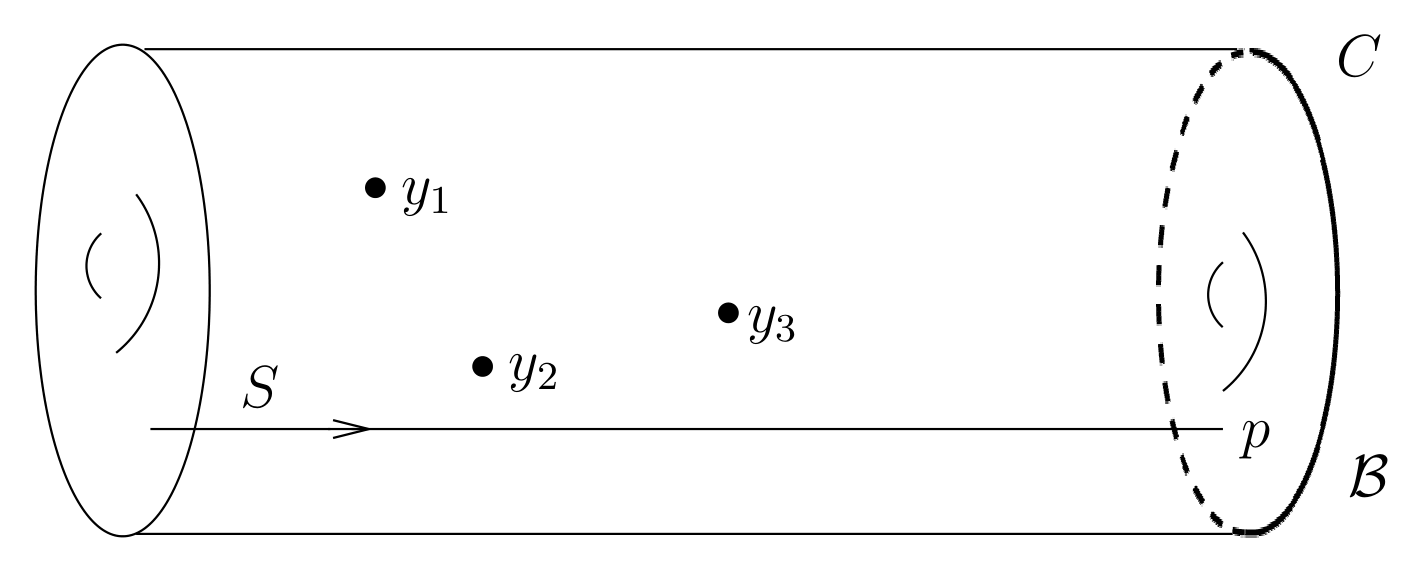
\includegraphics[width=0.62\linewidth]{figures/figure-2.png}
  \caption{时间无关情形的零时刻切片。面算符的支撑 $D$ 与零时刻切片的交为直线 $S$；若干线算符的支撑 $L_i$ 与零时刻切片交于点 $y_i$（$i=1,2,3$）。（原文 Fig.~2，PDF 第 111 页）}
  \label{fig:2}
\end{figure}


为简单起见，我们假定线算符（line operator）与面算符的支撑不依赖于时间。于是，只要说明 $W$ 中发生的情况，就能描述线算符与面算符的任何组态。时间无关的面算符支撑在二维流形 $D=\R\times S$ 上，其中 $S$ 是 $W$ 中的一条曲线。用于几何朗兰兹的分歧情形时，取 $S=I\times p$，其中 $p$ 是 $C$ 中的一点。我们还纳入支撑为 $L_i=\R\times y_i$ 的线算符，其中 $y_i\in W$ 是若干点。这些线算符将简记为 $L_i$。该组态如图~\ref{fig:2} 所示。

\begin{yizhu}[物理图像补充]
时间无关（time-independent）的假设并不失一般性：在拓扑场论中时间方向没有动力学，任意算符组态都可以沿时间方向推挤；若某个线算符或面算符的支撑在时间方向上只有有限延展，它就给出作用在膜上的算符（见上文脚注）。取 $\Sigma=\R\times I$ 后，$W=I\times C$ 是一个圆柱（图~\ref{fig:2}）；$S=I\times p$ 是沿圆柱的一条母线，其两端落在 $W$ 的两个边界上，因此面算符的支撑 $D=\R\times S$ 终止于边界，必须并入“膜”的定义，而不是作为作用在膜上的算符。这正是原文强调面算符与线算符地位不同的原因：线算符的支撑 $L_i=\R\times y_i$ 可以把端点推到边界，从而成为作用在膜上的算符，而面算符的支撑本身就终止于边界。
\end{yizhu}

线算符可以理解为作用在膜上的算符，详见 \cite{ref8} 第 6.4 节。例如，利用拓扑不变性，我们可以移动点 $y_i$，使其趋近图~\ref{fig:2} 中标记为膜 ${\mathcal B}$ 的右边界。当 $y_i$ 趋近边界时，相应的线算符 $L_i$ 作用在 ${\mathcal B}$ 上，给出一个新膜 ${\mathcal B}_i$，我们把它符号地记为 $L_i\cdot {\mathcal B}$。相反，由于 $S=I\times p$ 终止于 $W$ 的边界，支撑在 $D=\R\times S$ 上的面算符必须作为“膜”这一概念的定义的一部分；在这种情形下，它并不真正给出一个作用在膜上的算符。\footnote{若某线算符或面算符的支撑在时间方向上只有有限延展，则它会给出一个作用在膜上的算符。}

拓扑不变性意味着存在一个自然的平坦联络，使得支撑在点 $y_i\in W$ 处的线算符自然等价于支撑在邻近点 $y_i'$ 处的线算符。由此可知线算符彼此对易，因为三维流形中一个小开集内互异点位的组态空间是连通且单连通的。连通性意味着我们可以让两个线算符彼此穿过而不会遇到奇点；单连通性则意味着（在同伦意义下）如何这样做没有歧义。

\bigskip\noindent{\it 支撑在曲面上的线算符}


% [FIGURE 3] 原文 PDF 第 112 页；caption 见下，需翻译
\begin{figure}[htbp]
  \centering
  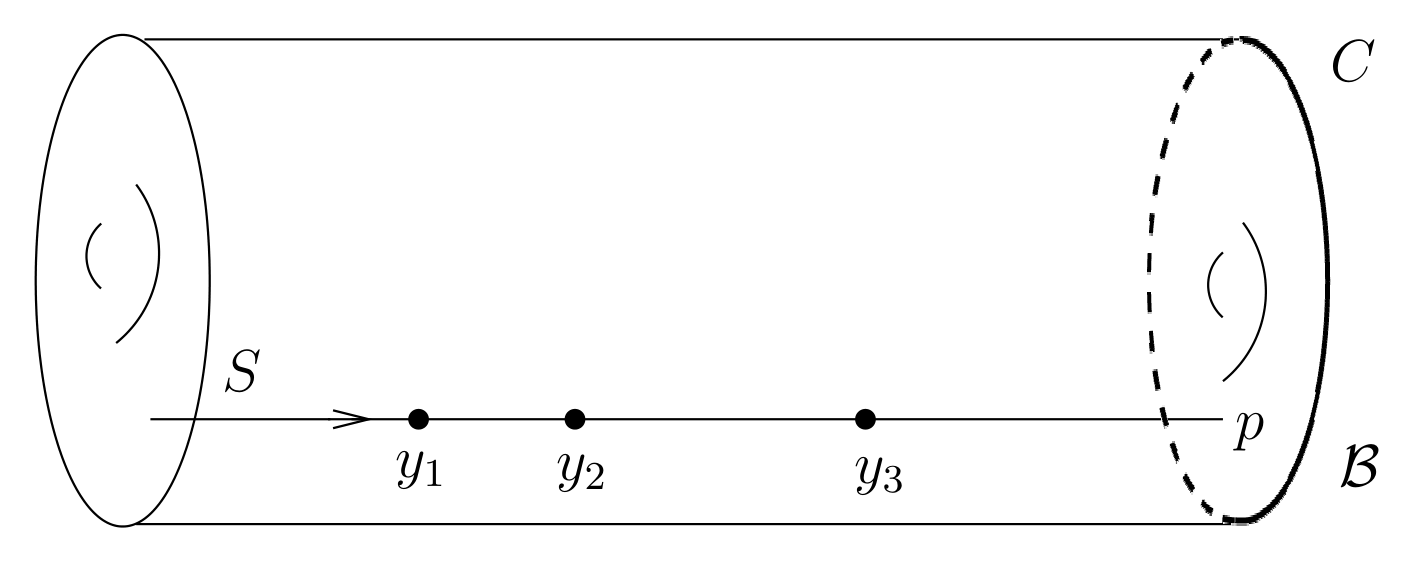
\includegraphics[width=0.62\linewidth]{figures/figure-3.png}
  \caption{支撑在曲面 $D$ 上的线算符 $L_i$。图中画出的是时间无关情形的零时刻切片；在零时刻，$D$ 由所示的直线 $S$ 表示，线算符则由 $S$ 上的点 $y_i$ 表示。（原文 Fig.~3，PDF 第 112 页）}
  \label{fig:3}
\end{figure}


然而现在考虑某些点 $y_i$ 实际落在曲线 $S$ 上的情形。在刚才的情形中，若取 $y_i=u_i\times p$，其中 $u_i\in I$、$p$ 是 $C$ 中的分歧点，就会出现这种情形（图~\ref{fig:3}）。此时，直线 $L_i=\R\times y_i$ 当然包含在曲面 $D=\R\times S$ 内，于是我们得到的是一个支撑在曲面上的线算符。当然，在给定面算符的支撑上允许何种线算符，是我们必须处理的一个问题。

支撑在曲面上的线算符与四维空间中的一般线算符颇为不同，因为只要定向适当，它们就具有自然的次序。图~\ref{fig:3} 画出了这一点，其中的次序为 $y_1<y_2<y_3$。支撑为 $\R\times y_i$ 的线算符给出一个作用在膜上的算符，因为我们可以把点 $y_i$ 向右移动，此时相应的线算符便作用在膜 ${\mathcal B}$ 上。然而一般来说，不应期望支撑在膜上的线算符彼此对易，因为它们有确定的次序，而且无法在不相遇奇点的情况下彼此穿过。

于是，在一般点 $q\in C$ 处，我们得到一个由作用在膜上的威尔逊算符或 't Hooft 算符构成的交换代数 ${\mathcal S}_{q}$。但在分歧点 $p$ 处，一般得到的是一个非交换代数 $\hat {\mathcal S}_p$。

尽管 $\hat {\mathcal S}_p$ 一般是非交换的，但它与支撑在一般点 $q\in C$ 处的威尔逊算符或 't Hooft 算符构成的代数 ${\mathcal S}_{q}$ 对易。道理很简单：只要 $q$ 不是分歧点，作用在 $q$ 处的线算符就可以自由地向左或向右移动，而不会遇到奇点。

\begin{yizhu}[易错点]
线算符与面算符的支撑是几何上不同的对象：一般线算符的支撑是 $L_i=\R\times y_i$（四维中的一条线，在零时刻切片上是点 $y_i$），面算符的支撑是 $D=\R\times S$（四维中的一个曲面，在切片上是曲线 $S$）。当 $y_i\in S$ 时 $L_i\subset D$，即线算符位于面算符的支撑之内；这类“支撑在曲面上的线算符”沿 $S$ 有自然次序（图~\ref{fig:3}，$y_1<y_2<y_3$），不能互相穿过，因此一般不对易。相反，$C$ 上一般点处的线算符可以自由移动，故交换。两种情形不可混为一谈：$\hat {\mathcal S}_p$ 的非交换性来自面算符支撑上的次序结构，而不是来自四维整体的拓扑。
\end{yizhu}

当然，非交换代数可能包含很大的中心。令 $q$ 趋近 $p$ 取极限，就可以把 ${\mathcal S}_{q}$ 映入 $\hat {\mathcal S}_p$ 的中心。在拓扑场论中，这一极限必定存在，因为 $q$ 与 $p$ 之间的距离本来就没有意义。不过，一般而言，当 $q$ 绕 $p$ 转过一周时会出现单值性；一旦如此，${\mathcal S}_{q}$ 中元素当 $q\to p$ 时的极限就依赖于逼近的方向。对 $B$-模型这一点是显然的（我们在第~\ref{sec:5.2}~节会提到），对 $A$-模型则已在 \cite{ref75} 中作了分析（所用的语言与本文颇为不同）。

因此，通常的威尔逊算符或 't Hooft 算符代数可以映入作用在分歧点处的非交换代数的中心，但并不完全以典范的方式。

\bigskip\noindent{\it 与单值性的关系}

下面讨论这一表述与第~\ref{sec:4.5}~节中用单值性所作描述之间的关系。在那种做法中，人们考虑的是只保持一个拓扑超对称的膜上操作——即复结构 $J$ 下 $B$-模型的对称性，或辛结构为 $\omega_K$ 的 $A$-模型的对称性。为简单起见，我们只以 $B$-模型来表述下面的论证。对 $A$-模型，只需把 $\alpha$ 与 $\eta$ 互换，情况完全相同。

在复结构 $J$ 下的 $B$-模型中，拉格朗日量对 Kähler 参数 $(\beta,\eta)$ 的依赖完全呈 $\int_M d^4x\sqrt g \{Q,V\}$ 的形式，其中 $Q$ 是相应的拓扑超荷，$V$ 选取适当。对控制复结构的参数 $(\alpha,\gamma)$ 的依赖则无法写成这种形式。

适当选取 $V$ 后，我们可以让 $(\beta,\eta)$ 这一对量成为沿面算符的支撑 $D$ 非常数的函数。就本文的目的而言，我们取这些函数不依赖于时间，但沿图~\ref{fig:3} 的曲线 $S$ 从左向右移动时发生变化。我们必须避开使量子理论变得奇异的那些 $(\beta,\eta)$ 取值。让 $(\beta,\eta)$ 沿 $S$ 变化并避开奇点轨迹，恰好重现第~\ref{sec:4.5}~节所描述的单值性。

现在可以看出单值性与线算符之间的关系。描述一个单值性时，可以令 $(\beta,\eta)$ 在某个小线段 $I_0\in S$ 之外为常数。在拓扑场论中，线段 $I_0$ 的长度无关紧要。若把该线段看作实质上是一个点，那么单值性不过是描述线算符的一种特殊方式。

然而，如果我们想看到 $\Psi=\infty$ 处 $B$-模型的全部拓扑超对称，用单值性来描述线算符就有缺陷。我们记得，这一对称性属于 $(B,B,B)$ 型。为了保持复结构 $J$ 下的 $B$ 型超对称，必须保持 $\alpha$ 与 $\gamma$ 固定（如上所做），因为该复结构依赖于这些参数。同样，为了保持复结构 $I$ 下的 $B$ 型超对称，必须保持 $\beta$ 固定，因为复结构 $I$ 依赖于 $\beta$。所以总的来说，要保持 $(B,B,B)$ 型的全部拓扑超对称，我们只能变化 $\eta$；而即便如此，最多也只能看到对应于把 $\eta$ 平移一个格矢量的阿贝尔单值性。

最有趣的非阿贝尔奇点预期出现在 $\alpha=\beta=\gamma=0$ 时。此时为避免奇点，$\eta$ 必须是正则的；于是 $\eta$ 被限制在一个仿射外尔房（affine Weyl chamber）的内部。在这一限制下，我们根本观察不到任何单值性。

当然，在 $\Psi=0$ 的 $A$-模型中，若想看到 $(B,A,A)$ 型的全部拓扑超对称，也有类似的问题。要保留问题的全部对称性，单值性就不是一个合适的框架。本节余下部分的目标是：看看改为从线算符而非单值性出发——也就是定义与非分歧情形中威尔逊算符和 't Hooft 算符类似的离散操作——能做得比单值性好多少。

\subsection{\texorpdfstring{$B$-模型}{B-模型}}

%% ==== 原文 §5.2：PDF 第 115 页（印刷第 114 页）====
\label{sec:5.2}

容易讨论的是 $B$-模型，但也正是在这一情形中我们无法得到完全令人满意的答案。

在非分歧情形，规范群为 $^L\neg G$ 时，作用在膜上的重要算符是 $^L\neg G$ 的表示 $^L\neg R$ 中的威尔逊算符。它们由复值联络 $\CA=A+i\phi$ 的平行移动（parallel transport）来定义。若 $L$ 是四维流形 $M$ 中的闭圈，则威尔逊算符定义为
% 式 (5.1)
\setcounter{equation}{0}
\begin{equation}\label{eq:5.1}
  W({}^L\neg
R;L)=\Tr\,P\exp\left(-\int_L\CA\right),
\end{equation}
 其中 $P\exp\left(-\int_L\CA\right)$ 是联络 $\CA$ 沿直线 $L$ 的和乐，迹在表示 $^L\neg R$ 中取。若 $L$ 改为一条开线（连接 $M$ 的边界或端点），则把 $W({}^L\neg R;L)$ 定义为此和乐，并将它视为在表示 $^L\neg R$ 的初态与末态之间作用的算符。

对非分歧情形的几何朗兰兹纲领，取 $M=\R\times I\times C$，其中 $\R$ 参数化“时间”，$I$ 是一个区间，$C$ 是黎曼面。要得到能作用在膜上的威尔逊算符，取 $L=\R\times u\times q$，其中 $u\in I$ 与 $q\in C$ 是选定的点。

若 $L$ 包含在面算符的支撑 $D$ 内（如图~\ref{fig:3}），我们可以作几乎相同的构造。但有一个重要差别：在面算符的支撑上，群 $^L\neg G$ 被约化为其极大环面 $^L\neg \TT$。因此，若 $L$ 包含在 $D$ 内，我们可以定义与 $^L\neg \TT$ 的表示的选择相应的威尔逊算符。这比选择 $^L\neg G$ 的表示更为一般，因为 $^L\neg G$ 的表示可以分解为 $^L\neg \TT$ 的表示的直和，但反过来一般不行。

因此一般说来，在分歧点处，$^L\neg \TT$ 的表示环（representation ring）作用在 $\Psi=\infty$ 处模型的膜上，从而推广了一般点处由 $^LG$ 的表示给出的作用。其发生方式很简单：与 $^LG$ 的表示相联系的、位于一般点 $q$ 的威尔逊算符，在 $q$ 趋近 $p$ 的极限下分裂为与 $^L\neg \TT$ 的表示相联系的威尔逊算符之和。

由于 $B$-模型的分歧平坦丛绕面算符的支撑具有单值性，这一情形中 $q\to p$ 的极限有微妙之处：极限依赖于人们让 $q$ 逼近 $p$ 所走的路径。

\bigskip\noindent{\it 解释}

$^L\neg \TT$ 的表示环就是余权格（coweight lattice）$\Lambda_\cowt$。其中包含一个由不改变离散电通量 ${\bf e}_0$ 的威尔逊算符组成的子格 $\Lambda_\cort$（余根格，coroot lattice）。

\begin{yizhu}[含糊点拨]
$^L\neg \TT$ 的表示环之所以等于余权格 $\Lambda_\cowt$，是因为 $\TT$ 与 $^L\neg \TT$ 互为对偶环面：$\TT$ 的余特征格正是 $^L\neg \TT$ 的特征格，而环面的不可约表示由特征（权）标号；等价地说，$^L\neg \TT$ 的表示环是以 $\Lambda_\cowt$ 为基的格代数。子格 $\Lambda_\cort$ 则对应不改变离散电通量 ${\bf e}_0$ 的那些威尔逊算符。原文没有展开的是：这一“表示环作用”与第~\ref{sec:4.5}~节由单值性给出的“格 $\Lambda_\cort$ 或 $\Lambda_\cowt$ 的作用”是同一件事的两种描述，其等价性依赖下面式~\eqref{eq:5.2} 的二维阿贝尔结果。
\end{yizhu}

我们在第~\ref{sec:4.5}~节中也遇到过格 $\Lambda_\cort$ 或 $\Lambda_\cowt$ 在膜上的作用。不过那里的解释稍有不同：在那种做法中，格的作用是平移 $\eta$，也就是把定义在杂质曲面（impurity surface）上的 $\theta$ 角平移 $2\pi$。

不过，一个经典结果 \cite{ref76} 表明：二维阿贝尔规范场论中的威尔逊算符会使 $\theta$ 角平移 $2\pi$ 的整数倍。下面回顾它是怎么来的。考虑二维流形 $D$ 上规范群为 $H=U(1)$ 的规范场论。取 $L$ 为 $D$ 上一条适当类型的一维流形。最简单的情形是 $L$ 为区域 $R\subset D$ 的边界，且是一条闭一维流形。设 $A$ 是 $D$ 上曲率为 $F$ 的阿贝尔规范场\footnote{我们把 $A$ 视为主 $U(1)$ 丛上的联络，局部地用实一维形式表示。}。则 $A$ 绕 $L$ 的和乐满足恒等式

% 式 (5.2)
\setcounter{equation}{1}
\begin{equation}\label{eq:5.2}
  \exp\left(i\oint_LA\right)=\exp\left(i\int_RF\right).
\end{equation}

这说明，在穿过支撑着电荷为 1 的威尔逊算符的那条线时，$\theta$ 角跳跃 $2\pi$。若分析得更仔细，即使一维流形 $L$ 不闭合，也能得到同样的结论。

\begin{yizhu}[易错点]
式~\eqref{eq:5.1} 与式~\eqref{eq:5.2} 的符号约定不同：式~\eqref{eq:5.1} 中 $\CA=A+i\phi$ 是复值联络，威尔逊线按本文约定取 $P\exp(-\int_L\CA)$（与 $D=d+A$、和乐 $P\exp(-\int A)$ 一致）；而式~\eqref{eq:5.2} 讨论的是按数学约定写成的 $U(1)$ 实一维形式 $A$，故用 $\exp(i\oint_LA)$。两者相差因子 $i$ 与符号，比较前必须统一约定。式~\eqref{eq:5.2} 的物理含义是：穿过电荷为 1 的威尔逊算符所在的线时 $\theta$ 角跳跃 $2\pi$；这也解释了为什么面算符支撑上“格的作用”既可看成表示环的作用，也可看成 $\eta$ 的平移（后者正是 $\theta$ 角的 $2\pi$ 平移）。
\end{yizhu}

\bigskip\noindent{\it 讨论}

因此，对于正则半单型单值性的情形，我们用规范场论找到的格在膜上的作用，就是我们预期能看到的全部。然而，按第~\ref{sec:4.5}~节的分析，当对 $(\alpha,\gamma)$ 非正则时，应当有一个更大的非交换群作用在膜上。遗憾的是，正如我们下面要说明的，在 $\Psi=\infty$ 处似乎很难用半经典规范场论方法看到这一更大的对称性。因此，用这些方法我们实际上无法比用单值性做得更好。

我们想看到的单值性来自 $\beta$ 与 $\eta$ 的变化；若把 $\beta$ 约束住，使三元组 $(\alpha,\beta,\gamma)$ 恒为正则，这些单值性就不存在。所以这些单值性的存在取决于该三元组变为非正则时发生的情况。此时，用第~\ref{sec:3.6}~节的话说，经典模空间 $\MH$ 会出现局部奇点。

这些单值性仍然有意义，因为只要 $\eta$ 是一般的，量子理论就保持光滑。然而，在线算符的半经典规范场论构造中，很难利用量子理论的这一事实。任何这类构造都从经典构造出发，然后在量子层面实现。定义依赖于理论量子性质的算符，用规范场论方法很难看到。

在 $A$-模型中情况不同，因为 $\alpha$ 与 $\eta$ 的角色互换了。相应的单值性通过在固定 $\gamma$ 与 $\eta$ 的同时变化 $\alpha$ 与 $\beta$ 而得到。即使 $\gamma=\eta=0$，只要 $(\alpha,\beta)$ 处于正则区域，就能看到全部单值性；而这意味着 $\MH$ 的经典几何是光滑的。

这提示我们，在 $A$-模型中，用规范场论方法描述作用在膜上的全部算符以及它们所保持的全部超对称，可能会更成功。这将是我们下一个目标。


%% ============================================================
%% 片段：s05b-amodel   对应原文 PDF 第 117--129 页
%% 本文件由 gw/convert.py 从 arXiv 源码（hep-th/0612073v2）自动生成：
%%   * 公式/编号/引用/图 已经锁定为原文内容，请勿改动任何数学内容与编号；
%%   * 只需把英文正文译为中文，并在每节开头加“本节重点”、关键处加译注。
%% ============================================================


\subsection{\texorpdfstring{$A$-模型}{A-模型}}

%% ==== 原文 §5.3：PDF 第 117 页（印刷第 116 页）====
\label{sec:5.3}

在没有分歧时，$A$-模型中作用于膜上的自然算符是 't Hooft 算符，其定义方式是规定场必须满足的奇点。因此，在有分歧时，我们将寻找类 't Hooft 算符（'t Hooft-like operators）。为简单起见，我们取定义面算符的列维子群（Levi subgroup）为 $\mathbb{L}=\TT$。

要得到 $\Psi=0$，即具有辛结构 $K$ 的 $A$-模型，一个方便的做法是取底层四维理论的扭曲参数（twisting parameter）为 $t=1$，并令四维 $\theta$ 角为零。在一般四维流形 $M$ 上，保持 $A$-模型拓扑对称性的条件已在 \cite{ref8} 的式 (9.1)、(9.2) 中描述。若令 $\CA=A+i\phi$，并记 $\CF=d\CA+\CA\wedge \CA$ 为 $\CA$ 的曲率、$d_A=d+A$，则条件为

% 式 (5.3)
\setcounter{equation}{2}
\begin{equation}\label{eq:5.3}
  \begin{aligned}\CF+i\star \overline\CF & = 0\\
                    d_A\star \phi & = 0.\end{aligned}
\end{equation}


我们具体取 $M=\R\times W$，其中 $\R$ 由“时间”坐标 $s$ 参数化。我们把方程~\eqref{eq:5.3} 限制到与时间无关的情形。其动机在于：通常的 't Hooft 算符由与时间无关的奇点定义（另外也基于 \cite{ref8} 第 9 节引论部分给出的论证，那些论证在有分歧时同样适用）。在与时间无关的情形下，四维联络约化为 $A=A'+A_0\,ds$，其中 $A'$ 是 $G$-丛 $E\to W$ 上的联络，$A_0$ 是取值于 ${\rm ad}(E)$ 的零形式。类似地，写 $\phi=\phi'+\phi_0\,ds$，其中 $\phi'$ 与 $\phi_0$ 是 $W$ 上取值于 ${\rm ad}(E)$ 的形式。令 $\CA'=A'+i\phi'$、$\CF'=d\CA'+\CA'\wedge \CA'$、$\Phi_0=\phi_0-iA_0$。由于此后全部讨论都在三维中进行，我们略去撇号。式~\eqref{eq:5.3} 中的第一个方程变为

% 式 (5.4)
\setcounter{equation}{3}
\begin{equation}\label{eq:5.4}
  \CF=\star\bar {\mathcal D}\Phi_0,
\end{equation}

其中 $\bar{\mathcal D}=d+\bar\CA$，而 $\star$ 此时当然是三维的霍奇 $\star$ 算符。第二个方程变为

% 式 (5.5)
\setcounter{equation}{4}
\begin{equation}\label{eq:5.5}
  D\star \phi={i\over 2}[\bar\Phi_0,\Phi_0].
\end{equation}


\bigskip\noindent{\it 标度对称性}

类 't Hooft 算符用这些方程的奇异解来定义。例如，通常的 't Hooft 算符所用的奇异解在余维三处有奇点，即在孤立点 $r\in W$ 处。该构造在 \cite{ref8} 第 6.2 节中描述过，下面将加以推广。在本文中，我们的主题一直是面算符，它由指定一个余维二奇点——即带有参数 $(\alpha,\beta,\gamma)$ 的熟知奇点——而产生。


% [FIGURE 4] 原文 PDF 第 118 页；caption 见下，需翻译
\begin{figure}[htbp]
  \centering
  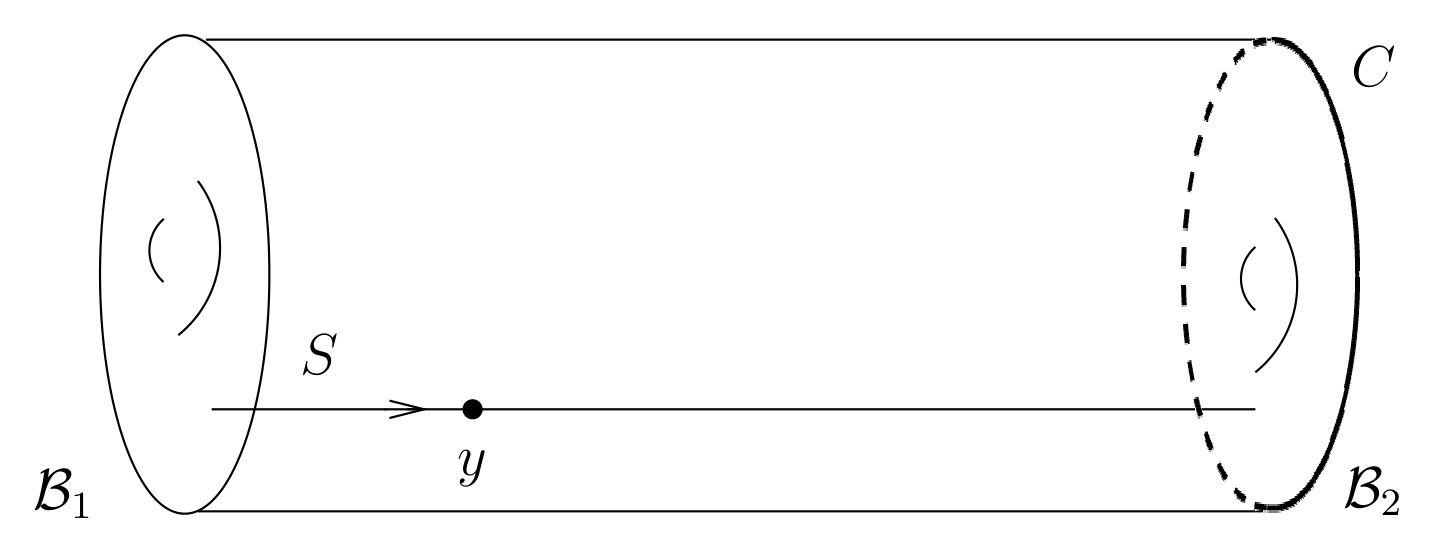
\includegraphics[width=0.62\linewidth]{figures/figure-4.png}
  \caption{支撑在曲面上的线算符，在这一零时刻切片上由直线 $S$ 上的一个点 $y$ 表示。在 $A$-模型中，场沿 $S$ 具有指定的奇点。在 $y$ 附近，奇异行为与 $S$ 上一般点附近的不同。而沿 $S$ 的一般奇异行为，在 $y$ 的两侧又可能不同。（原文 Fig.~4，PDF 第 118 页）}
  \label{fig:4}
\end{figure}

我们感兴趣的是更复杂的情形：一条由余维二奇点构成的曲线 $S$ 含有孤立点 $y$，在该点奇异行为“更糟”。因此，在 $S$ 的一般点附近看到的是通常的余维二奇点，而在点 $y\in S$ 处出现新的奇点。\emph{先验地}，在 $y$ 的左侧，直线 $S$ 由参数 $(\alpha,\beta,\gamma)$ 标记，而在右侧由参数 $(\alpha',\beta',\gamma')$ 标记。若要得到保持 $(B,A,A)$ 型全部超对称的面算符，必须有 $(\beta,\gamma)=(\beta',\gamma')$，因为 $\beta$ 与 $\gamma$ 是 $I$ 型 $B$-模型中的物理参数；要保持该模型的超对称，它们就不能跳变。然而，没有理由只考虑 $\alpha=\alpha'$ 的情形。$(B,A,A)$ 型的拓扑场论局部地与 $\alpha$ 无关，因此应当预期所得到的结果本质上不依赖于 $\alpha$ 与 $\alpha'$。
\begin{yizhu}[易错点]
为什么 $(\beta,\gamma)$ 不能跳而 $\alpha$ 可以跳？根据表~\ref{tab:1} 中复模与 Kähler 模的分配即可看清：$(B,A,A)$ 中唯一的 $B$-模型是 $I$ 型，它只依赖复结构 $I$ 的模 $\beta+i\gamma$，故 $\beta,\gamma$ 是该模型的物理参数，跨过线算符时必须连续；所用的两个 $A$-模型是 $J$ 型与 $K$ 型，它们分别只依赖辛类，而对应的 Kähler 模分别是 $\beta$（在 $J$ 中）与 $\gamma$（在 $K$ 中）。至于 $\alpha$，它在 $I$ 中是 Kähler 模（$I$ 型 $B$-模型不看 Kähler 类），在 $J$ 中是复模 $\gamma+i\alpha$、在 $K$ 中是复模 $\alpha+i\beta$（$A$-模型不看复结构），因此 $\alpha$ 不进入 $(B,A,A)$ 的任何一项，可以在 $y$ 两侧取不同值 $\alpha,\alpha'$。这也正是后文总把 $\beta,\gamma$（以及量子的 $\eta$）与 $\alpha$ 区别对待的原因。
\end{yizhu}

% [FIGURE 5] 原文 PDF 第 119 页；caption 见下，需翻译
\begin{figure}[htbp]
  \centering
  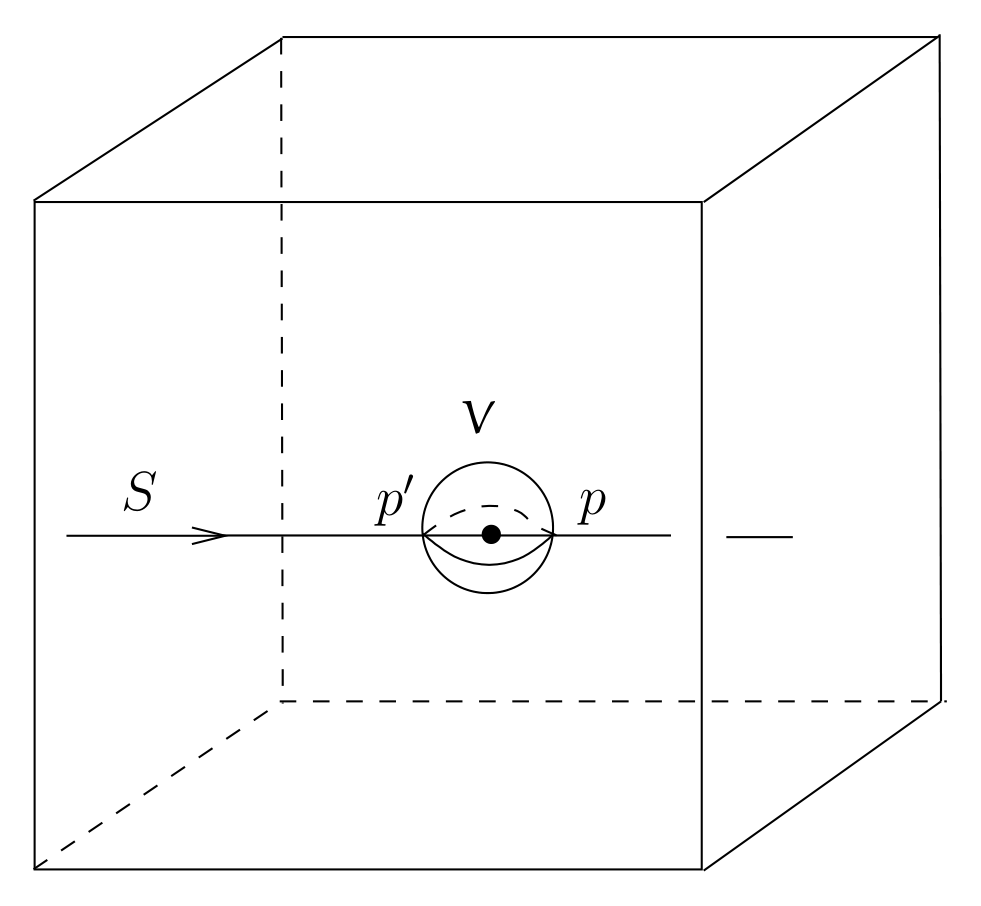
\includegraphics[width=0.62\linewidth]{figures/figure-5.png}
  \caption{为局部地描述该奇点，我们把三维流形 $W$ 换为 $\R^3$，把直线 $S$ 换为 $\R^3$ 中的一条直线 $\R$。点 $y$ 成为 $\R^3$ 的原点，图中以黑点标出。$\EURV$ 是包围原点的单位球面，它与直线 $S$ 交于两点 $p$ 与 $p'$。（原文 Fig.~5，PDF 第 119 页）}
  \label{fig:5}
\end{figure}

为简化，我们对所要寻找的奇点的性质作一假设。假定它们是标度不变的，正如用来定义通常 't Hooft 算符的奇点那样。的确，由于只关心局部的奇异行为，可以把 $W$ 换为 $\R^3$，并以 $y$ 为 $\R^3$ 的原点。在 $\R^3$ 上取欧氏坐标 $x^1,x^2,x^3$，并把图~\ref{fig:5} 中的直线 $S$ 取为 $x^1$ 轴，即由 $x^2=x^3=0$ 定义的那条轴。$\R^3$ 具有标度对称性 $\vec x\to \lambda \vec x$，$\lambda$ 取实正值。所关心的方程在这一标度对称性下不变（若取 $\Phi_0$ 的量纲为 1 来标度），而沿 $S$ 在远离 $y$ 处所需的奇点与标度不变性相容。因此寻找标度不变的奇异解是有意义的，而这已足以满足此处之需。


若从 $\R^3$ 中挖去点 $y$ 再按标度作商，得到 $(\R^3\backslash y)/\R^*_+=S^2\cong \mathbb{CP}^1$。我们称这个商为 $\EURV$。有意思的解大体上可以用 $\EURV$ 上的数据来描述。$\EURV$ 上的场将在图~\ref{fig:5} 所示的两点处奇异，即 $\EURV$ 与直线 $S$ 相交的点 $p$ 与 $p'$。

\bigskip\noindent{\it $\phi=0$ 的情形}

如第~\ref{sec:4.5}~节所述，若 $\beta=\gamma=0$，作用于膜上的算符最为有趣。此时可以取 $\phi=0$（因为 $\phi$ 沿 $S$ 的一般点并无奇点）。结果表明，我们所寻求的类 't Hooft 算符可以用同时满足 $\phi=0$、$A_0=0$ 的奇异解来定义。

这使方程~\eqref{eq:5.4} 与~\eqref{eq:5.5} 大大简化。它们约化为 Bogomolny 方程（Bogomolny equations）

% 式 (5.6)
\setcounter{equation}{5}
\begin{equation}\label{eq:5.6}
  F=\star d_A\Phi_0,
\end{equation}
 其中此时 $F=dA+A\wedge A$、$\Phi_0=\phi_0$ 取值于 $G$ 的实李代数 $\mathfrak g$。我们作一个比标度不变性更强的假设：$A$ 与 $\Phi_0$ 都是从 $\EURV=S^2$ 拉回的。把 $\EURV$ 视为 $\R^3$ 中的单位球面，即由 $r=1$ 定义，其中 $r=|\vec x|$。在 $S^2$ 上得到的方程为
% 式 (5.7)
\setcounter{equation}{6}
\begin{equation}\label{eq:5.7}
  \begin{aligned}F&=-\star\Phi_0\\
                  d_A\Phi_0&=0,\end{aligned}
\end{equation}

                  其中此时这些是二维流形 $\EURV$ 上的方程，$\star$ 取二维意义。例如，为得到第一个方程，我们利用 $\Phi_0$ 对 $r$ 的依赖恰为因子 $1/r$（因 $\Phi_0$ 按权重 1 标度），于是在 $r=1$ 处有 $\partial\Phi_0/\partial r = -\Phi_0$。第二个方程则利用了 $F$ 与 $\partial/\partial r$ 缩并时为零这一事实（因为我们假定解是从 $\EURV$ 拉回的）。

\begin{yizhu}[易错点]
从三维的 $F=\star d_A\Phi_0$ 降到 $\EURV$ 上时，$\star_2\Phi_0$ 前的负号来自 $\star$ 算符的分解而非方程本身：以 $r=|\vec x|$ 为法向，有 $\star_3\omega_2=dr\wedge\star_2\omega_2$ 与 $\star_3(dr\wedge\omega_1)=\star_2\omega_1$；又 $\Phi_0$ 按权重 1 标度，即 $\Phi_0=r^{-1}\Phi_0^{(2)}$，故 $d_A\Phi_0$ 含 $-r^{-1}dr\,\Phi_0^{(2)}$ 一项。代入~\eqref{eq:5.6} 并在 $r=1$ 处分离分量：$dr$ 分量给出 $d_A\Phi_0=0$，纯二维分量给出 $F=-\star_2\Phi_0$。因此~\eqref{eq:5.7} 第一式的负号是 $\star$ 的维数改变带来的，把两式当成同一个方程照抄就会把它丢掉。
\end{yizhu}


显然，两式合起来给出
% 式 (5.8)
\setcounter{equation}{7}
\begin{equation}\label{eq:5.8}
  d_A\star F=0.
\end{equation}

这就是二维杨–米尔斯方程，即由杨–米尔斯作用量导出的欧拉–拉格朗日方程
% 式 (5.9)
\setcounter{equation}{8}
\begin{equation}\label{eq:5.9}
  {\bm{I}}=-{1\over
2}\int_\EURV\,\,\Tr \,F\wedge \star F.
\end{equation}


这些方程还有如下解释。给定黎曼面 $\EURV$，$G$-丛 $E\to
\EURV$ 上的每个联络 $A$ 都赋予 $E$ 一个全纯结构，它由 $\bar\partial$ 算符 $\bar \partial_A=d\bar z(\partial_{\bar z}+A_{\bar
z})$ 定义。反过来，也可以从全纯
$G_\C$-丛 $E\to \EURV$ 出发，问 $E$ 容许哪些与其全纯结构相容的酉联络（相容是指由该联络诱导的全纯结构与 $E$ 给定的全纯结构一致）。稳定与半稳定丛正是那些容许与其全纯结构相容的平坦酉联络的丛 \cite{ref51}。更一般地，若给 $\EURV$ 配上 Kähler 度量从而有 $\star$ 算符（使得杨–米尔斯方程与作用量有定义），则据 \cite{ref52}，每个 $G_\C$-丛 $E\to \EURV$（无论稳定与否）都容许一个酉联络，它在规范变换下唯一，满足杨–米尔斯方程并与 $E$ 的全纯结构相容。于是特别地，模去规范变换的杨–米尔斯方程解，与全纯 $G_\C$-丛的等价类自然对应。

这一结果在杨–米尔斯作用量的梯度流（gradient flow）\cite{ref52} 中有自然的解释，但此处不需要。对我们更重要的是把上述结果推广到容许抛物结构的情形 \cite{ref77}。我们将对任意数目的分歧点、任意选取的抛物子群陈述这一定理。从黎曼面 $\EURV$ 中挖去有限个点 $p_1,\dots,p_s$。给每个 $p_i$ 标上一个抛物权（parabolic weight）$\alpha_i \in \mathfrak t$，以及相联系的共轭类 $U_i=\exp(-2\pi\alpha_i)$。假定 $\alpha_i$ 足够一般，使得对每个 $i$，与 $\alpha_i$ 交换的列维子群 $\mathbb{L}_i\subset G$ 与和 $U_i$ 交换的子群相同；记 ${\EUP}_i$ 为由配对 $(\mathbb{L},\alpha_i)$ 决定的抛物子群。考虑 $G$-丛 $E\to \EURV\backslash
\{p_1,\dots,p_s\}$ 上满足杨–米尔斯方程的联络 $A$，它绕点 $p_i$ 的和乐与 $U_i$ 共轭。该断言是：这样的联络（模去规范变换）与在点 $p_i$ 处具有（$\EUP_i$ 型）抛物结构的全纯 $G_\C$-丛 $E\to \EURV$ 一一对应。抛物丛稳定或半稳定，当且仅当对应的杨–米尔斯方程解是平坦的；否则它是不稳定的。
\begin{yizhu}[含糊点拨]
作者把“Bogomolny 方程 $\to$ 二维杨–米尔斯方程 $\to$ 全纯丛／抛物丛”这条链当作已知结果引用（\cite{ref51,ref52,ref77}），其中被略去的论证是：二维杨–米尔斯方程 $F=-\star\Phi_0$、$d_A\Phi_0=0$ 合起来即 $d_A\star F=0$，也就是曲率（等价地 $\star F$）协变常；在紧黎曼面上，满足杨–米尔斯方程的酉联络模去规范变换，恰好给出全纯 $G_\C$-丛的模空间（Narasimhan–Seshadri 定理的微分几何形式），稳定／半稳定丛对应解的存在性；带抛物结构时（Mehta–Seshadri、Biquard 等的定理 \cite{ref77}），对应的解析对象是带抛物权与抛物型约化的全纯丛，平坦解对应稳定抛物丛。正是这一定理链条，使我们可以用 $\mathbb{CP}^1$ 上两点处的抛物丛来分类类 't Hooft 算符。
\end{yizhu}

在应用这一定理时，由于我们取面算符为 $\TT$ 型，眼下关心的是各 $\mathbb{L}_i$ 都与极大环面 $\TT$ 共轭的情形。因此，在本节末尾简要讨论一般 $\mathbb{L}$ 型面算符之前，“抛物结构”一词都指把结构群约化到博雷尔子群（Borel subgroup）$\EUB$。

\bigskip\noindent{\it $SL(2,\C)$ 的抛物丛}

为构造类 't Hooft 算符，我们关心 $\EURV=\mathbb{CP}^1$ 上在两点 $p$ 与 $p'$ 处具有抛物结构的 $G_\C$-丛。这两点处的抛物权为 $\alpha$ 与 $-\alpha'$。出现负号的原因是：在图~\ref{fig:5} 中，二维球面 $\EURV$ 与直线 $S$ 在点 $p$ 与 $p'$ 处以相反的定向相交。
\begin{yizhu}[易错点]
图~\ref{fig:5} 的几何是理解两个点（puncture）$p$、$p'$ 的关键：$\EURV$ 是 $\R^3$ 中以原点（即点 $y$）为中心的单位球面，直线 $S$（$x^1$ 轴）穿过球心，故与 $\EURV$ 交于两点 $p$、$p'$，二者互为对径点（图中 $p'$ 在左、$p$ 在右，箭头给出 $S$ 的定向）。$S$ 的定向在穿过球心的两侧相对球面给出相反的指向，于是在 $p$ 与 $p'$ 处测得的奇异参数相差一个符号，抛物权写作 $\alpha$ 与 $-\alpha'$；若算符两侧参数不跳（$\alpha=\alpha'$），两点处的权就是 $\alpha$ 与 $-\alpha$。这也解释了单值性公式 $U=\exp(-2\pi\epsilon\alpha)$、$U'=\exp(2\pi\epsilon'\alpha')$ 中 $\epsilon'$ 带来的符号自由度。
\end{yizhu}

这种情形下的抛物丛可以非常具体地描述。为说明关键思想，取 $G_\C=SL(2,\C)$，并同时从全纯的观点和利用与杨–米尔斯方程的关系来进行分析。

从全纯观点看，$SL(2,\C)$ 丛 $E\to \EURV$（视为行列式平凡、秩为 2 的向量丛）必为 $\CO(m)\oplus \CO(-m)$，其中 $m$ 为某整数，不妨假定它非负。此外，还必须在两点 $p,p'\in
\EURV$ 处给 $E$ 配上抛物结构。对黎曼面上给定点处的秩 2 丛 $E$，抛物结构不过是在该点处 $E$ 的纤维中选取一个一维子空间。记这两处的纤维为 $E|_p$ 与 $E|_{p'}$。于是点 $p$ 与 $p'$ 处的抛物结构由子空间 $E_p\subset E|_p$ 与 $E_{p'}\subset E|_{p'}$ 的选取给出。这类抛物丛的同构类可如下分类：

(1) 先设 $m=0$。此时丛 $E$ 平凡，群 $G_\C\cong
SL(2,\C)$ 作用于其上。若 $E$ 存在一个非零整体截面，其到 $p$ 的限制取值于 $E_p$、到 $p'$ 的限制取值于 $E_{p'}$，我们就说 $p$ 与 $p'$ 处的抛物结构一致。否则说它们不一致。在同构意义下，即模去 $SL(2,\C)$ 的作用，恰有两种选择：$p$ 与 $p'$ 处的抛物结构或者一致，或者不一致。

(2) 现在设 $m>0$。丛 $E=\CO(m)\oplus \CO(-m)$ 有唯一的子丛同构于 $\CO(m)$（其特征是：$E$ 的任意整体全纯截面实际上都是这个子丛的截面）。相比之下，$\CO(-m)$ 在 $E$ 中的嵌入、从而分裂 $E=\CO(m)\oplus \CO(-m)$ 并非典范的。模去 $E$ 的自同构，抛物结构中唯一的不变量信息是：子空间 $E_p$ 与 $E_{p'}$ 是否与 $\CO(m)$ 在 $p$ 与 $p'$ 处的纤维重合。因此对给定的 $m$，共有 $2\times 2=4$ 种选择。我们把这四种可能组织如下。若 $E_p=\CO(m)|_p$，就用整数 $m$ 标记抛物丛 $E$；否则用 $-m$ 标记它。并且，若 $E_p$ 与 $E_{p'}$ 或者都与 $\CO(m)$ 的相关纤维重合、或者都与它不同，我们就说 $p'$ 处的抛物结构与 $p$ 处的一致。否则说抛物结构不一致。

现在从杨–米尔斯方程的观点来看。此时需要在点 $p$ 与 $p'$ 处选取抛物权。（这些权没有进入全纯描述，因为我们并不关心哪些抛物丛稳定。）取

% 式 (5.10)
\setcounter{equation}{9}
\begin{equation}\label{eq:5.10}
  \begin{aligned}\alpha&=iy\,\left(\begin{matrix}1 & 0\\ 0&-1\end{matrix}\right)\\
\alpha'&=iy'\,\left(\begin{matrix}1 & 0\\ 0&-1\end{matrix}\right),\end{aligned}
\end{equation}

其中 $0<y,y'<1/2$。初始时取 $y\not=y'$ 也较为方便。

杨–米尔斯方程~\eqref{eq:5.8} 表明曲率是协变常的，因此可以选取一个规范使曲率实际上是常数
% 式 (5.11)
\setcounter{equation}{10}
\begin{equation}\label{eq:5.11}
  F=i\left(\begin{matrix}f & 0\\ 0 &
-f\end{matrix}\right),
\end{equation}
 其中 $f$ 为实常数，不妨取非负。稍后就会看到，若 $y\not=
y'$ 则 $f\not=0$。由于 $F$ 协变常，它与绕点 $p$ 与 $p'$ 的和乐 $U$、$U'$ 交换，因此（假定 $f\not=0$）这些和乐是对角矩阵。由于和乐必须分别与 $\exp(-2\pi\alpha)$ 和 $\exp(-2\pi (-\alpha'))$ 共轭，于是 $U=\exp(- 2\pi\epsilon \alpha)$、$U'=\exp(2\pi\epsilon'\alpha')$，其中 $\epsilon,\epsilon'=\pm 1$。

最后，具有上述联络与曲率的丛 $E$ 存在，当且仅当

% 式 (5.12)
\setcounter{equation}{11}
\begin{equation}\label{eq:5.12}
  \exp\left(\int_{\EURV}F\right)=UU'.
\end{equation}
 该条件等价于
% 式 (5.13)
\setcounter{equation}{12}
\begin{equation}\label{eq:5.13}
  \int_\EURV{f\over 2\pi}+\epsilon
y-\epsilon' y'= m',
\end{equation}
 其中 $m'$ 为某整数。

\begin{yizhu}[物理图像补充]
式~\eqref{eq:5.12} 是 Stokes 定理在 $\EURV$ 上的体现：绕 $p$ 与 $p'$ 的两个小圈之和与绕整个 $\EURV$ 的大圈同调，故绕大圈的和乐 $\exp(\int_{\EURV}F)$ 等于两个小圈的和乐之积 $UU'$（不计一次共轭，视基点而定）。把它对角化即得~\eqref{eq:5.13}：$\int_{\EURV}f/2\pi+\epsilon y-\epsilon'y'=m'\in\Z$，其中 $m'$ 是本征值所对应的整数，$\epsilon,\epsilon'$ 是 $\alpha$ 与 $-\alpha'$ 的权同 $\pm y$ 的配对符号。给定 $y,y'$ 与 $\epsilon,\epsilon'$ 后，整数 $m'$ 唯一决定 $\int_{\EURV}f/2\pi\ge 0$，即决定曲率的大小。
\end{yizhu}

外尔群通过改变 $F$、$y$、$y'$ 与 $m'$ 的符号来作用。因此，经一个外尔变换可固定 $\epsilon=1$；此后杨–米尔斯方程的解由整数 $m'$ 与变量 $\epsilon'\in\{\pm 1\}$ 标记。我们所给出的杨–米尔斯方程解的分类在 $y=y'$ 时同样成立，但此时处理 $\epsilon'=1$、$m'=0$ 的情形需要稍加小心。

\begin{yizhu}[含糊点拨]
「稍加小心」指的是 $f=0$ 这一支。~\eqref{eq:5.13} 中 $f\ge 0$，故 $f=0$ 当且仅当 $m'=\epsilon y-\epsilon'y'$；而 $0<y,y'<1/2$ 使 $\epsilon y-\epsilon'y'\in(-1,1)$，又必须是整数，于是 $f=0$ 只发生在 $y=y'$、$\epsilon=\epsilon'$、$m'=0$ 时。此时 $U'=\exp(2\pi\epsilon'\alpha')=\exp(2\pi\alpha)=U^{-1}$，故 $UU'=1$，与~\eqref{eq:5.12} 相容；反过来若固定 $\epsilon=1$ 而取 $\epsilon'=-1$（仍 $y=y'$），则 $U'=U$、$UU'=\exp(-4\pi\alpha)\ne 1$，与~\eqref{eq:5.12} 矛盾，该支并不存在。上文「假定 $f\ne 0$ 故和乐为对角矩阵」的论证在 $f=0$ 时确实失效。
\end{yizhu}

于是，杨–米尔斯解的分类与抛物丛的分类一致。在这一比较中，$m'$ 对应于 $m$，而 $\epsilon'=1$（或 $-1$）对应于两处抛物结构一致（或不一致）的情形。

每个这样的解或丛都使我们能够定义一个类 't Hooft 算符。于是，对每一对 $(m,\epsilon')\in \Z\times \Z_2$ 都得到一个类 't Hooft 算符 $T_{m,\epsilon'}$。

这些算符确实保持 $(B,A,A)$ 型的全部拓扑超对称。为看出这一点，首先注意：由于它们来自所需方程~\eqref{eq:5.4} 与~\eqref{eq:5.5} 的解，它们保持 $K$ 型 $A$-模型（具有辛结构 $\omega_K$ 的那个）的拓扑对称性。由于这些解在 $\varphi\to i\varphi$ 下不变，而该变换把辛结构 $\omega_K$ 旋转为 $\omega_J$，它们也保持 $J$ 型 $A$-模型的拓扑对称性。这两个超荷的线性组合生成 $(B,A,A)$ 型的全部拓扑超对称。
\begin{yizhu}[易错点]
$(B,A,A)$ 型超对称的含义是：在复结构 $I$ 上取 $B$-模型，在复结构 $J$ 与 $K$ 上取 $A$-模型。本节从 $\Psi=0$ 出发：按第~\ref{sec:5}~节，$\Psi=0$ 一侧的拓扑场论是 $\MH$ 上辛结构 $\omega_K$ 的 $A$-模型（而另一端点 $\Psi=\infty$ 给出复结构 $J$ 上的 $B$-模型）。$A$-模型只依赖辛结构（复化 Kähler 类）而与复结构无关，于是本段的论证分两步：解来自~\eqref{eq:5.4}、\eqref{eq:5.5}，故保持 $K$ 型 $A$-模型的拓扑对称性；解又在 $\varphi\to i\varphi$ 下不变，而该操作把 $\omega_K$ 旋转为 $\omega_J$，故也保持 $J$ 型 $A$-模型的拓扑对称性；两个超荷的线性组合即生成完整的 $(B,A,A)$。易错之处：$\varphi\to i\varphi$ 并非解的对称性，而是把 $K$ 型解映为同形式的 $J$ 型解（后文纳入 $\beta,\gamma$ 时还会用到这一点）。
\end{yizhu}


\bigskip\noindent{\it 在膜上的作用}


% [FIGURE 6] 原文 PDF 第 124 页；caption 见下，需翻译
\begin{figure}[htbp]
  \centering
  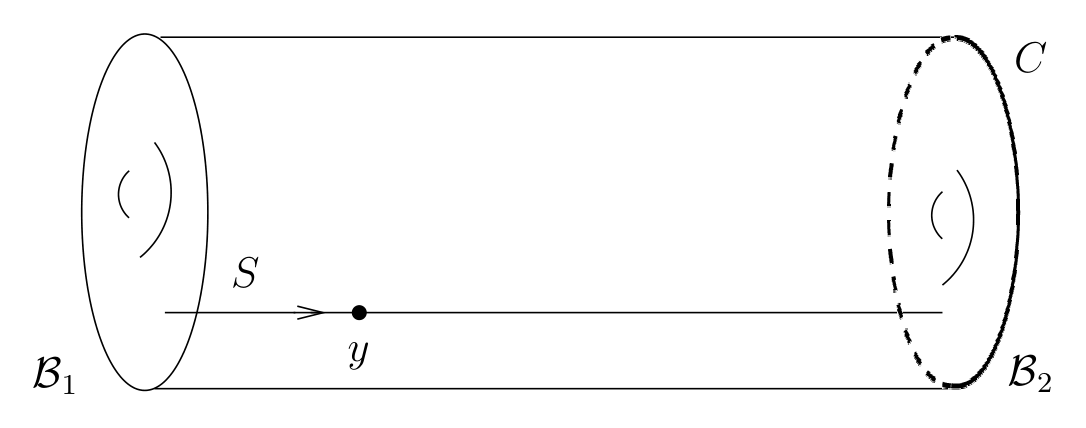
\includegraphics[width=0.62\linewidth]{figures/figure-6.png}
  \caption{线算符（此处插入在点 $y$）在膜上的作用。场 $(A,\phi)$ 对每个 $u\in S$ 都在复结构 $I$ 中确定一个带分歧的希格斯丛 $E_u\to C_u=\{u\}\times C$。在超对称方程的解中，$E_u$ 的全纯类型为常数，除非 $C_u$ 越过点 $y$——越过时它发生跳变。（原文 Fig.~6，PDF 第 124 页）}
  \label{fig:6}
\end{figure}

粗略地说，这些类 't Hooft 算符之一在膜上的作用，类似于无分歧情形中通常 't Hooft 算符的作用，如 \cite{ref8} 所述。因此我们只作相当简略的说明。


在图~\ref{fig:6} 中，我们考虑三维流形 $W=I\times C$ 上 $G$-丛 $E$ 的场 $(A,\phi)$，它们沿直线 $S$ 具有通常的奇点。对任意 $u\in I$，把丛 $E$ 与场 $A,\phi$ 限制到 $C_u=\{u\}\times C$，得到带分歧的希格斯丛 $E_u\to C_u$。若满足 Bogomolny 方程~\eqref{eq:5.6}，则 $E_u$ 的全纯类型与 $u$ 无关，除非越过某个线算符所在的位置。若越过的是支撑在 $C$ 中一般点（乘 $I$ 中一点）处的线算符，则丛 $E_u$ 经历通常的 Hecke 修改；而若如图~\ref{fig:6} 那样越过支撑在 $S$ 上的线算符，则得到更一般的类 Hecke 修改，它可以涉及抛物结构。这些陈述的理由与 \cite{ref8} 中相同。

现在设我们想看出图~\ref{fig:6} 中点 $y$ 处的线算符 $L_y$ 如何作用在，比如说，图左侧的膜 ${\mathcal B}_1$ 上。刚才所述意味着算符 $L_y$ 确定一个“对应”${\EUQ}\subset \MH\times \MH$。$\EUQ$ 参数化对 $(\tilde E_u,E_u)$，其中 $\tilde E_u$ 可由 $E_u$ 通过“跳过”线算符 $L_y$ 得到。$\EUQ$ 可视为 $\MH\times \MH$ 中 $(B,A,A)$ 型的膜，因为它由保持该对称性的方程之解得到。我们主要把它看作 $K$ 型的 $A$-膜。

事实上，可用来定义类 't Hooft 算符 $L_y$ 的 $\EURV\cong \mathbb{CP}^1$ 上的抛物丛大多是不稳定的。出现这种情况时，我们实际上希望用配对 $(\tilde E_u, E_u)$ 的空间作紧化来定义 $\EUQ$，即把用不那么不稳定的抛物丛（对 $G_\C=SL(2,\C)$ 来说就是 $|m|$ 更小）所定义的类 Hecke 修改也包括进去。这与无分歧情形完全类似。可以预期，原则上这种紧化的使用能由底层的四维规范场论来论证。

现设 $\pi_i$（$i=1,2$）为两个投影 $\pi_i:\MH\times\MH\to \MH$。给定 $\MH$ 上的膜 ${\mathcal B}_1$，我们把它经 $\pi_1^*$“拉回”到 $\MH\times \MH$，与 $\EUQ$ 作张量积，再经 $p_{2}$“前推”到 $\MH$，得到新的膜 $L_y\cdot {\mathcal B}_1$。即 $L_y\cdot {\mathcal B}_1=\pi_{2\,*}(p_1^*({\mathcal B}_1)\otimes
\EUQ)$。若 ${\mathcal B}_1$ 是 $(B,A,A)$ 型的膜，这些运算可以用复结构 $I$ 中的复几何来实施；但更一般地，若 ${\mathcal B}_1$ 只是 $K$ 型的 $A$-膜，则必须使用这些运算在 $A$-模型中的类比，即在 Floer 上同调中的类比。
\begin{yizhu}[原文疑误]
原文此处（PDF 第 125 页）刚把两个投影定义为 $\pi_1,\pi_2$，紧接着却说经 $p_2$“前推”，并在同一公式中写出 $p_1^*$，同时又用 $\pi_{2\,*}$；由上下文看 $p_1,p_2$ 与 $\pi_1,\pi_2$ 指同一对投影，应是原文的记号笔误。译文照原文保留 $p_1,p_2$，不作改动。另：图~\ref{fig:6} 的 caption 写作“对每个 $u\in S$”，而正文为“对任意 $u\in I$”——$S$ 是 $W=I\times C$ 中沿时间方向的直线，两者可理解为把 $u$ 记作沿 $S$ 的时间参数；译文亦照原文保留。
\end{yizhu}


下面给出一个或许更朴素的解释。为构造图~\ref{fig:6} 情形下的物理希尔伯特空间（两端由膜给出边界条件、内部有算符 $L_y$），可如下进行。考虑超对称位形的紧化模空间 $\bar{\mathcal N}$，其边界条件由两端的膜 ${\mathcal B}_1$、${\mathcal B}_2$ 以及内部的 $L_y$ 确定。物理希尔伯特空间是 $\bar{\mathcal N}$ 的上同调。为定义 $L_y$ 在膜上的作用，其想法是：$\bar{\mathcal N}$ 的上同调，与去掉 $L_y$ 造成的奇点、并把 ${\mathcal B}_1$ 换为另一个膜 $L_y\cdot{\mathcal B}_1$（它将不依赖于 ${\mathcal B}_2$）之后所得到的上同调相同。$L_y\cdot{\mathcal B}_1$ 的 Chan–Paton 层（Chan-Paton sheaf）在点 $E_u\in\MH$ 处的纤维，等于按如下方式得到的空间 $\Xi(E_u)$ 的上同调：$\Xi(E_u)$ 参数化希格斯丛 $\tilde E_u$，使得对 $(\tilde E_u,E_u)$ 代表 $\EUQ$ 中的一个点。（在这个过分简化的解释中，我们忽略了 $\EUQ$ 的奇点。）只要仔细考虑有、无算符 $L_y$ 插入时物理希尔伯特空间如何计算，就可以为这一方案提供论证。

\begin{yizhu}[物理图像补充]
公式 $\pi_{2,*}(\pi_1^*(\mathcal B_1)\otimes\EUQ)$ 就是由核 $\EUQ$ 给出的积分变换。在 $I$ 型 $B$-模型里，$\mathcal B_1$ 是 $\MH$ 上的相干层复形，$\otimes$ 取导出张量积、$\pi_{2,*}$ 取导出推前，这正是 Fourier--Mukai 型函子；而导出推前在点 $E_u$ 处的纤维恰为 $R\Gamma(\Xi(E_u),\cdot)$，其全上同调即文中说的「$\Xi(E_u)$ 的上同调」。换到 $K$ 型的 $A$-模型，$\MH$ 的辛结构使膜成为 $\omega_K$-拉格朗日膜，$\EUQ$ 成为拉格朗日对应，$\otimes$ 换成纤维积、$\pi_*$ 换成 Floer 复形，这就是段末所说「在 Floer 上同调中的类比」。
\end{yizhu}


\bigskip\noindent{\it 仿射外尔群与辫群}

现在回到 $G_\C=SL(2,\C)$ 的例子，其中我们把类 't Hooft 算符按对 $(m,\epsilon')\in \Z\times\Z_2$ 作了分类。$SL(2,\C)$ 的仿射外尔群 $\AffWeyl$（已在式~\eqref{eq:3.50} 中引入）是一个扩张
% 式 (5.14)
\setcounter{equation}{13}
\begin{equation}\label{eq:5.14}
  0\to \Z\to \AffWeyl\to\Z_2\to 0,
\end{equation}
 而该群的元素相当自然地由配对 $(m,\epsilon')$ 标记，正如类 't Hooft 算符那样。实际上，由于 $\Z_2$ 通过变号作用于 $\Z$，$m$ 的符号有一点微妙之处，正如 't Hooft 算符那里的情形一样。't Hooft 算符与 $\AffWeyl$ 的元素之间的对应，比二者中任何一个与配对 $(m,\epsilon')$ 的对应都更自然。

\begin{yizhu}[物理图像补充]
对 $G=SL(2,\C)$，式~\eqref{eq:5.14} 就是无限二面体群的正合列：由~\eqref{eq:3.50}，$\AffWeyl=\Lambda_{\rm cort}\rtimes\Weyl$，此处 $\Lambda_{\rm cort}\cong\Z$、$\Weyl=\Z_2$，故 $\AffWeyl\cong\Z\rtimes\Z_2$。$\Z_2$ 的生成元把平移 $m$ 共轭为 $-m$，这正是文中「$m$ 的符号有一点微妙之处」的来源：$(m,\epsilon')$ 与 $(-m,\epsilon')$ 是两个不同的群元素，须先选定 $\epsilon'$ 的代表元，标号才唯一；也正因如此，算符与 $\AffWeyl$ 的元素之间的对应，比它与 $(m,\epsilon')$ 的对应更自然。
\end{yizhu}

对任意单连通的 $G$ 有类似的结论：$\mathbb{CP}^1$ 上恰在两点处具有抛物结构的丛，自然地对应于 $\AffWeyl$ 的元素。这在杨–米尔斯进路中相当容易看出：把我们对 $SL(2,\C)$ 给出的论证加以推广即可，故留作练习。这在全纯进路中也是一个标准结果。\footnote{它等价于如下陈述：$\mathbb{CP}^1$ 上在两点处具有抛物结构的丛，对应于 Iwahori 群在仿射旗流形上作用的轨道。}



% [FIGURE 7] 原文 PDF 第 127 页；caption 见下，需翻译
\begin{figure}[htbp]
  \centering
  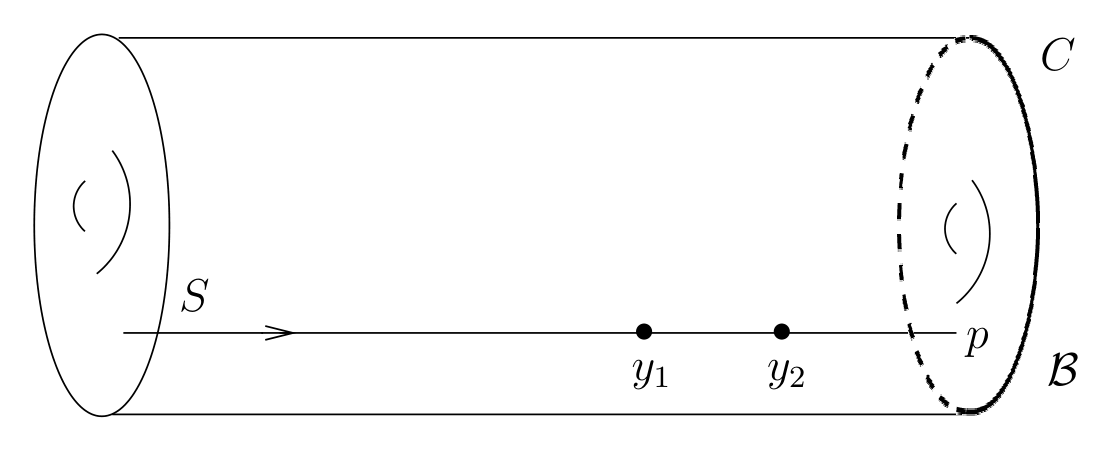
\includegraphics[width=0.62\linewidth]{figures/figure-7.png}
  \caption{共存于某个面算符的支撑上的两个线算符，可以通过简单地把两条线移到一起而复合。在此描绘的静态情形中，这通过取 $y_1\to y_2$ 的极限来实现。在拓扑场论中，线算符生成一个作用于膜的结合代数。（原文 Fig.~7，PDF 第 127 页）}
  \label{fig:7}
\end{figure}

我们所定义的类 't Hooft 算符可以通过把两条线移到一起而以自然方式复合，如图~\ref{fig:7} 所示。或许会预期这些算符按仿射外尔群的乘法法则复合。然而，据 \cite{ref29} 以及我们在第~\ref{sec:4.5}~节中的论证，应当预期：在分歧点 $p\in C$ 处作用于 $A$-模型之膜的群是仿射辫群（affine braid group），而不是仿射外尔群。如式~\eqref{eq:4.16} 那样，两个群由一个正合列相联系
% 式 (5.15)
\setcounter{equation}{14}
\begin{equation}\label{eq:5.15}
  1\to
\pi_1(\eurz)\to B_{\rm aff}\to \AffWeyl\to 1,
\end{equation}
 其中 $\eurz$ 是 $\AffWeyl$ 自由作用的空间，由配对 $(\alpha,\beta)\in \mathfrak t\times \mathfrak t$ 构成。这是一个非平凡扩张，因此 $\AffWeyl$ 可以提升到 $B_{\rm aff}$，但这样的提升不保持群运算。因此，我们不预期作用于膜上的算符 $T_{m,\epsilon'}$ 尊重仿射外尔群的这些关系。

\begin{yizhu}[易错点]
式~\eqref{eq:5.15} 的 $\AffWeyl$、$B_{\rm aff}$ 没有标注 ${}^L$，而第~\ref{sec:4.5}~节的式~\eqref{eq:4.16} 明写作 $B_{\rm aff}({}^L\neg G)$、$\AffWeyl({}^L\neg G)$；第~4.5~节那里讨论 $Y=1$ 的情形，$\eurq_Y$ 是 $\bar\TT_\C$ 的正则点、其商是 $\bar G_\C$ 的正则共轭类空间，所得的群按定义就是 ${}^L\!G$ 的仿射辫群（该节译注已指出该处 ${}^L$ 标注与邻近约定略有出入）。两处 $\eurz$ 其实是同一个空间，即 $\AffWeyl$ 自由作用的正则序对 $(\alpha,\beta)\in\mathfrak t\times\mathfrak t$；本节讨论 $\mathbb{CP}^1$ 上两点的抛物 $G_\C$-丛与 't Hooft 算符，故按 $G$ 标号。两列形式相同而群不同，不可混用；译文照原文保留。
\end{yizhu}

可以稍微具体一些。对秩为 $r$ 的 $G$，$\AffWeyl$ 由基本反射 $T_i$（$i=1,\dots,r+1$）生成，Dynkin 图的每个节点对应一个。它们满足 $T_i^2=1$ 以及某些附加关系。例如，对秩大于 1 的单边型（simply-laced）$G$，若顶点 $i$ 与 $j$ 由一条边相连，则

% 式 (5.16)
\setcounter{equation}{15}
\begin{equation}\label{eq:5.16}
  T_iT_jT_i=T_jT_iT_j
\end{equation}

若不相连，则

% 式 (5.17)
\setcounter{equation}{16}
\begin{equation}\label{eq:5.17}
  T_iT_j=T_jT_i
\end{equation}

要得到仿射辫群，只需去掉关系 $T_i^2=1$，保留其余关系。仿射外尔群中长度最短的词，可以相当自然地提升为仿射辫群中的“同一个”词，但这并不给出群同态。

\begin{yizhu}[含糊点拨]
「不能给出同态」的精确含义是~\eqref{eq:5.15} 作为群扩张不可裂：若存在同态 $s:\AffWeyl\to B_{\rm aff}$ 使 $B_{\rm aff}\to\AffWeyl$ 与之合成为恒等，则 $\AffWeyl$ 的每个关系在 $B_{\rm aff}$ 中都成立，特别地 $T_i^2=1$ 成立；但仿射辫群恰恰是删去 $T_i^2=1$、保留~\eqref{eq:5.16} 与~\eqref{eq:5.17} 得到的，其中 $T_i^2\ne 1$。故原文的「非平凡扩张」应读作「不分裂」：最短词给出的是集合论截面，只保证辫关系成立，不保证群运算，这正是「不预期算符 $T_{m,\epsilon'}$ 尊重仿射外尔群的关系」的意思。
\end{yizhu}


这里我们不试图用规范场论方法描述对应于 $\pi_1(\eurz)$ 的在膜上的运算。在例子中，$\pi_1(\eurz)$ 似乎通过把膜的 Chan–Paton 丛与某些具有非平凡鬼数（ghost number）作用的向量丛作张量积来作用。

\begin{yizhu}[易错点]
两套 $T$ 记号不要混：$T_i$（$i=1,\dots,r+1$）是仿射 Dynkin 图节点所对应的基本反射，$T_{m,\epsilon'}$ 则是按 $\AffWeyl$ 的元素（由配对 $(m,\epsilon')$ 标号）命名的类 't Hooft 算符。生成元有 $r+1$ 个而非 $r$ 个；对 $G=SL(2,\C)$（$r=1$）只有 $T_1,T_2$，而 $\widehat{A_1}$ 的图是双边，不属于文中「秩大于 1 的单边型」，故~\eqref{eq:5.16} 不适用于此例：此时 $\AffWeyl\cong\Z\rtimes\Z_2$，除 $T_i^2=1$ 外并无辫关系，式~\eqref{eq:5.16} 只是单边型情形才有的「附加关系」。
\end{yizhu}



\bigskip\noindent{\it $\beta$ 与 $\gamma$ 的纳入}

到目前为止我们都取希格斯场 $\phi$ 为零，而这只有在 $\beta=\gamma=0$ 时才有意义。若 $(\beta,\gamma)\not=0$，则 $\phi$ 具有指定的奇点，不能为零。

把 $\beta$ 与 $\gamma$ 纳入分析出乎意料地直接，理由如下。我们用来描述算符 $T_{m,\epsilon'}$ 的杨–米尔斯方程解实际上全是阿贝尔的，即结构群从 $G$ 约化到其极大环面 $\TT$。这反映了挖去两点的二维球面的基本群是阿贝尔群这一事实。

既然如此，只需为 $\phi$ 显式地加上一个阿贝尔解，就能把 $\beta$ 与 $\gamma$ 纳入。给定 $(\beta,\gamma)\in \mathfrak t$，定义

% 式 (5.18)
\setcounter{equation}{17}
\begin{equation}\label{eq:5.18}
  \varphi =\half(\beta+i\gamma){dz\over z},
\end{equation}
 其中 $z=x^2+ix^3$，$x^2$ 与 $x^3$ 是直线 $S\subset W=\R^3$ 的法坐标。（$\varphi$ 不是从 $\EURV$ 拉回的。）于是令 $\phi=\varphi+\bar\varphi$（仍取 $A_0=0$），即满足方程~\eqref{eq:5.4} 与~\eqref{eq:5.5}。$\varphi$ 的奇点与 $x^1$ 无关；因此正如所预期的，这一构造只有在 $\beta$ 与 $\gamma$（不同于 $\alpha$）越过线算符的支撑时不跳变的前提下才可能。

\begin{yizhu}[物理图像补充]
能把 $A$ 与 $\varphi$ 直接叠加，靠的是解的阿贝尔性：'t Hooft 解中的 $A$、$\Phi_0$ 与这里的 $\beta,\gamma$ 都取值于 $\mathfrak t$，而 $[\mathfrak t,\mathfrak t]=0$，故 $\phi\wedge\phi=\sum_{a,b}\phi^a\wedge\phi^b[T_a,T_b]=0$、$[A,\phi]=0$、$[\bar\CA,\Phi_0]=0$，于是 $\CF$ 与 $\bar{\mathcal D}\Phi_0$ 都不因加上 $\varphi$ 而改变；又 $z\ne 0$ 时 $d\varphi=0$，故 $\phi=\varphi+\bar\varphi$ 自动满足~\eqref{eq:5.5}。若换成非阿贝尔解，$\CF$ 会多出 $-\phi\wedge\phi+i d_A\phi$，这一叠加就不成立，文中强调「阿贝尔解」正在于此。
\end{yizhu}

如此得到的线算符确实保持 $(B,A,A)$ 型的拓扑对称性。在移植我们在 $\varphi=0$ 处给出的论证时，只需注意一处。变换 $\varphi\to i\varphi$ 并不是刚才所述解的对称性，而是把该解映为具有不同 $(\beta,\gamma)$ 的同形式解。这已足以确立该论证。

以这种方式纳入 $\phi$，尽管看似平凡，实际上却对解中涉及规范场的部分施加了有趣的限制。（无分歧情形的类似陈述见 \cite{ref8} 第 10.5 节。）当 $\beta=\gamma=0$ 时，点 $p$ 与 $p'$ 处的抛物结构之间相差一个相对的外尔变换。例如，在杨–米尔斯构造中，出现这一情形是因为：知道单值性 $U_1$ 与 $U_2$ 的共轭类、连同它们与曲率 $F$ 交换这一事实，只能把二者确定到外尔变换为止。然而，外尔群对角地作用于三元组 $(\alpha,\beta,\gamma)$ 与 $(\alpha',\beta,\gamma)$。因此，既然 $\beta$ 与 $\gamma$ 固定，就不能用任意外尔变换作用于 $\alpha$ 与 $\alpha'$。我们只能使用在 $\beta$ 与 $\gamma$ 上平凡作用的外尔变换。在量子情形下，若纳入 $\eta$——它同样不能跳变，因为它是 $K$ 型 $A$-模型的物理参数——则外尔变换必须与 $(\beta,\gamma,\eta)$ 交换。因此，这种类型的面算符由特征类 $\mathfrak{m}$ 以及与 $(\beta,\gamma,\eta)$ 交换的一个外尔变换确定。这正是人们会从第~\ref{sec:4.5}~节预期的结果。\footnote{那里的分析给出了略有不同的答案（外尔变换须与 $(\gamma,\eta)$ 交换），因为那里只考虑 $K$ 型 $A$-模型，$\beta$ 可以自由变动；而此处我们构造的是保持完整 $(B,A,A)$ 对称性的类 't Hooft 算符。}

特别地，若三元组 $(\beta,\gamma,\eta)$ 正则，则完全没有作外尔变换的自由度。因此，作用于分歧点的类 't Hooft 算符完全由特征类 $\mathfrak{m}\in \Lambda_{\rm cort}$ 分类（若希望包括改变丛的特征类的算符，则取 $\mathfrak{m}\in \Lambda_{\rm cowt}$）。这与第~\ref{sec:4.5}~节的分析一致：那里我们发现，在具有正则半单单值性的分歧点情形，作用于膜的正是这个格。

\begin{yizhu}[含糊点拨]
$\Lambda_{\rm cort}$ 与 $\Lambda_{\rm cowt}$ 之别决定「算符能否改变丛的特征类」。由~\eqref{eq:3.50}，$\AffWeyl=\Lambda_{\rm cort}\rtimes\Weyl$；对单连通的 $G$ 余根格与余特征格相同，故 $\mathfrak m\in\Lambda_{\rm cort}$ 正是 $\mathbb{CP}^1$ 上 $G$-丛的拓扑标号（即平移部分）。若允许算符把丛变为特征类相差一个余权的丛（单极型跳跃），平移格须扩大为 $\Lambda_{\rm cowt}$；对单连通的 $G$，$\Lambda_{\rm cowt}/\Lambda_{\rm cort}\cong Z(G)$ 即中心。因此括号里的两种取法是同一分类在更大格上的推广，而不是两类不同的算符。
\end{yizhu}

\bigskip\noindent{\it $\mathbb{L}$ 型的类比}

一如往常，可以把这一切推广到基于任意列维子群 $\mathbb{L}$ 的面算符情形。细节相当明显，留作练习。我们只指出：支撑在 $\mathbb{L}$ 型曲面上、$\beta=\gamma=0$ 的类 't Hooft 算符，仍由 $\EURV\cong \mathbb{CP}^1$ 上在两点 $p$ 与 $p'$ 处具有抛物结构的 $G_\C$-丛来分类。不过现在，$p$ 与 $p'$ 处的抛物结构分别是 $\EUP$ 型与 $\EUP'$ 型，其中 $\EUP$ 与 $\EUP'$ 是由配对 $(\mathbb{L},\alpha)$ 与 $(\mathbb{L},-\alpha')$ 决定的 $G_\C$ 的抛物子群。带这类抛物结构的丛可以借助杨–米尔斯方程容易地分类，它们对应于第~\ref{sec:3.7}~节中称为 ${\mathcal W}_{{\rm aff},\mathbb{L}}$ 的群的元素。这个群通过在分歧参数空间中的单值性作用在 $\M_{H,\mathbb{L}}$ 的上同调上。这些类 't Hooft 算符的复合，预期给出第~\ref{sec:4.5}~节所述的类辫群。纳入 $\beta$ 与 $\gamma$ 再次导致同样的效应：比较两个抛物结构时所涉及的外尔群元素必须与 $\beta$ 与 $\gamma$ 交换。


%% ============================================================
%% 片段：s06-local   对应原文 PDF 第 130--145 页
%% 本文件由 gw/convert.py 从 arXiv 源码（hep-th/0612073v2）自动生成：
%%   * 公式/编号/引用/图 已经锁定为原文内容，请勿改动任何数学内容与编号；
%%   * 只需把英文正文译为中文，并在每节开头加“本节重点”、关键处加译注。
%% ============================================================


\section{局部模型与弦论实现}

%% ==== 原文 §6：PDF 第 130 页（印刷第 129 页）====
\label{sec:6}

\begin{keytakeaways}
  \begin{itemize}[leftmargin=1.4em,itemsep=2pt,topsep=2pt]
    \item \textbf{物理图像}：面算符可用“局部模型”实现，即四维 ${\mathcal N}=4$ 超杨–米尔斯理论与支撑在二维子流形上的超对称西格玛模型的耦合；后者的靶空间为 $T^*(G/\mathbb{L})$，其超 Kähler 度量来自余伴随轨道。局部模型只适用于 $\MH$ 的局部奇点附近，且不保持 $S$-对偶。
    \item \textbf{数学工具}：$G_\C=SL(2,\C)$ 时用线性西格玛模型：$\mathbb{H}^2$ 的 $U(1)$ 超 Kähler 商给出 $A_1$ 奇点的超 Kähler 消解，Fayet–Iliopoulos 参数对应 $(\alpha,\beta,\gamma)$，$\theta$ 角对应 $\eta$；$O(2)$ 的非连通部分给出外尔群作用。
    \item \textbf{关键结论}：局部模型的单值群是轨形 $\tilde\C^*/\Z_2$ 的基本群；保持离散电通量 ${\bf e}_0$ 的子群恰为 $SL(2,\C)$ 的仿射辫群，这与第~\ref{sec:4.5}~节的结论一致。
    \item \textbf{瞬子图像}：局部模型在 $(\alpha,\beta,\gamma,\eta)=0$ 处的奇点来自小作用量瞬子级数在 $q=1$ 的极点；在四维中可用消没定理证明，只有 $\alpha/\gamma=(t-t^{-1})/2$、$\beta=0$ 时才存在这类瞬子。
    \item \textbf{弦论实现}：相交的 $D3$/$D3'$ 膜给出 $\mathbb{H}^N/\neg/\neg/U(1)$ 型线性西格玛模型，但破坏 $S$-对偶；改用 AdS/CFT（$AdS_5\times S^5$ 中的 $AdS_3\times S^1$）或 M 理论（$AdS_7\times S^4$ 中的 $M2$-膜）即可保持 $S$-对偶并获得面算符。
  \end{itemize}
\end{keytakeaways}


\subsection{概述}
%% ==== 原文 §6.1：PDF 第 130 页（印刷第 129 页）====
\label{sec:6.1}

本文的最后一节讨论若干前文主题的另类进路。我们先作一概览。

与其只靠假定场具有熟悉的奇点
% 式 (6.1)
\setcounter{equation}{0}
\begin{equation}\label{eq:6.1}
  \begin{aligned}A & =  \alpha \,d\theta \\
\phi & = \beta\,{dr\over r}-\gamma\,d\theta\end{aligned}
\end{equation}
（沿余维二的曲面 $D$）来描述面算符，人们自然会想用另一方式描述它：引入支撑在 $D$ 上的新自由度，并把它们与体（bulk）中 ${\mathcal N}=4$ 超杨–米尔斯理论的规范场耦合起来。例如，可把二维中具有 $(4,4)$ 超对称的超多重态（hypermultiplet）或向量多重态（vector multiplet）耦合到体中的 ${\mathcal N}=4$ 超杨–米尔斯理论。这样给出的理论，在某种程度上类似我们在本文中“手工”描述过的理论。

物理文献中当然已有许多关于共形场论与各种缺陷（defect）耦合的分析；所谓缺陷，即支撑在正余维子流形上的场。凝聚态物理中的 Kondo 模型（Kondo model）是一个经典例子。与当前关切更接近的是：定域在余维一的超多重态已通过膜构造（brane construction）与 ${\mathcal N}=4$ 超杨–米尔斯理论耦合，例如见 \cite{ref78,ref79}；而与我们最相关的余维二超多重态则已在 \cite{ref18} 中讨论过。

{}从第~\ref{sec:3.8}~节，我们其实可以看出什么样的杂质模型（impurity model）能重现我们所考虑的面算符的某些性质。本文的重要主题之一是希格斯丛模空间 $\MH$ 在三元组 $(\alpha,\beta,\gamma)$ 变为非正则时的“局部奇点”（local singularity）。这种局部奇点的超 Kähler 消解（hyper-Kähler resolution），可方便地用某些复余伴随轨道（coadjoint orbit）上的超 Kähler 度量~\cite{ref34} 来描述；等价地（在另一个复结构下），可用各列维子群 $\mathbb{L}\subset G$ 对应的 $X=T^*(G/\mathbb{L})$ 上的超 Kähler 度量来描述。因此，本文探讨的某些主题实际上可以用一个复合系统来表达：四维时空上的 ${\mathcal N}=4$ 超杨–米尔斯理论，加上支撑在时空的某个二维子流形上的超对称西格玛模型。我们称这个西格玛模型为局部模型（local model）。

尽管这一进路很有用，但据我们所知它有一个根本性的局限。本文发展的理论依赖于参数\footnote{为简洁起见，这里描述的是列维子群为 $\mathbb{L}=\TT$ 时的参数。一般地，所有参数都要求是 $\mathbb{L}$-不变的。} $(\alpha,\beta,\gamma,\eta)
\in \TT\times \mathfrak t\times\mathfrak t\times {}^L\neg\TT$。西格玛模型依赖于大体类似的参数 $(\alpha,\beta,\gamma,\eta)$：其中 $(\alpha,\beta,\gamma)$ 是进入 $X$ 上超 Kähler 度量的几何参数，$\eta$ 则包含西格玛模型的 $\theta$ 角。参数 $\eta$ 取值于 $^L\neg\TT$，与规范场论中一样（见式~\eqref{eq:3.44}）；同样，两种情形下 $\beta$ 与 $\gamma$ 都取 $\mathfrak t$ 值。但 $\alpha$ 在 $\MH$ 的完整几何中取 $\TT$ 值，而在 $T^*(G/\mathbb{L})$ 的超 Kähler 几何中取 $\mathfrak t$ 值（并通过 $SO(3)$ 对称性与 $\beta,\gamma$ 相联系），如我们在第~\ref{sec:3.8}~节回顾过的。因此，完整模型与局部模型的参数并不完全一致。

这与“局部模型刻画局部奇点附近行为”的说法并不矛盾，因为对这一目的而言，$\alpha$ 变大时的行为并不重要。然而，这显然意味着局部模型不可能具有 $S$-对偶。既然 $S$-对偶交换 $\alpha$ 与 $\eta$，它在靶为 $T^*(G/\mathbb{L})$ 的西格玛模型中就很难成立：在该模型中 $\eta$ 是角变量，而 $\alpha$ 取值于线性空间。因此，若把 ${\mathcal N}=4$ 理论耦合到这个局部模型，就不能指望保持 $S$-对偶。

这或许显得奇怪，但换一个观点也许会使该结论显得更自然。空间 $T^*(G/\mathbb{L})$ 不是环面纤维化，也不具有镜像对称（mirror symmetry），至少不具有 $G$-不变的镜像对称。（若西格玛模型的镜像对称不是 $G$-不变的，那么当它耦合到规范群为 $G$ 的四维规范场论时也帮不上多少忙。）因此，指望在把 ${\mathcal N}=4$ 超杨–米尔斯理论耦合到局部模型时仍保持 $S$-对偶，也许是不现实的。

尽管如此，正如我们强调过的，我们确实相信局部模型有助于研究 $\MH$ 的局部奇点附近（即非正则三元组 $(\alpha,\beta,\gamma)$ 附近）的行为。例如，考虑仿射辫群（affine braid group）$\BAff$ 在 $\Psi=\infty$ 处 $B$-模型的膜上的作用。在此作用中，$\alpha$ 与 $\gamma$ 保持固定（最有趣的情形是它们接近零），而研究的是关于 $\beta$ 与 $\eta$ 的单值性。$\alpha$ 取 $\mathfrak t$ 值还是 $\TT$ 值并不重要；$\BAff$ 作用于局部模型的 $B$-膜，其理由与它作用于 $\MH$ 上的膜相同。事实上，\cite{ref29} 中对 $\BAff$ 作用的分析，从物理观点看等价于研究局部模型 $B$-膜上的单值性作用。对于 $\MH$ 的 $B$-膜上的 $\BAff$ 作用，这似乎是一个好的局部模型。

相反，局部模型不是研究 $\Psi=0$ 处 $A$-膜上 $\BAff$ 作用的好模型。这涉及对 $(\alpha,\beta)$ 这对参数的单值性作用，而一旦 $\alpha$ 取 $\mathfrak t$ 值而非 $\TT$ 值，这一单值性作用就丢失了。据我们所知，要研究 $\MH$ 的 $A$-膜上的单值性作用，必须使用靶为 $\MH$ 的完整西格玛模型（或完整的四维规范场论）。这里有一个略带讽刺的角色反转：$A$-模型的单值性作用涉及经典辛同胚，而 $B$-模型的作用则高度非经典；但 $B$-模型的单值性作用可以在局部模型中研究，$A$-模型的却不能。

\bigskip\noindent{\it 本节内容}

现在我们可以简要概述本节内容。

正如已讨论的，尽管有局限，局部模型确有其用处。随之而来的问题是：是否存在关于局部模型的某种物理进路，使我们能比已获得的了解更多？对一般规范群我们尚无好的答案，但对 $G_\C=SL(2,\C)$ 的情形，局部模型有一个有用的描述。这将是第~\ref{sec:6.2}~节的主题。

第~\ref{sec:6.2}~节的分析将揭示一个事实的重要性：当三元组 $(\alpha,\beta,\gamma)$ 变为非正则时，（局部模型的某些超对称瞬子的）瞬子作用量消失。这一事实其实继承自四维规范场论中的类似事实，我们将在第~\ref{sec:6.3}~节说明。

最后，仅仅说局部模型缺少对偶对称性并不令人满意。我们能改用什么类似、但确实保持对偶对称性的做法？事实上，弦理论~\cite{ref18} 已在一个有趣的特别情形（$G_\C=SL(N,\C)$ 配以极小余伴随轨道）给出了这一问题的答案。我们在第~\ref{sec:6.4}~节说明。

\subsection{\texorpdfstring{$G_\C=SL(2,\C)$ 的线性西格玛模型}{G_C = SL(2,C) 的线性西格玛模型}}
 %% ==== 原文 §6.2：PDF 第 132 页（印刷第 131 页）====
\label{sec:6.2}

要利用局部模型——即靶为 $T^*(G/\mathbb{L})$ 的超对称西格玛模型——来学到四维规范场论中不明显的东西，我们需要一种不同的研究方式。我们没有对所有群一致适用的普遍方法，但将解释 $G=SU(2)$ 的一种有趣进路。这里我们依赖的事实是：唯一相关的 $\mathbb{L}$ 选取是 $\mathbb{L}=U(1)$，且 $T^*(SU(2)/U(1))=T^*\mathbb{CP}^1$ 是 $A_1$ 奇点的消解。因此，它可以构造为有限维线性空间的超 Kähler 商（hyper-Kähler quotient）~\cite{ref62}。这在膜物理中有许多应用~\cite{ref80}，且与我们的目的相关，因为可用它构造线性西格玛模型（linear sigma model）~\cite{ref81}，从而简单地理解靶为 $T^*\mathbb{CP}^1$ 的超对称西格玛模型的真空结构。

所有典型李群的复余伴随轨道同样可以构造为有限维线性空间的超 Kähler 商~\cite{ref82}。这些更一般的构造可以作为构造适用于任意典型群、与面算符相关的线性西格玛模型的起点。然而，$SU(2)$ 情形有一个重要优势：外尔群的作用在线性西格玛模型中一目了然。对更高秩的 $G$ 则并非如此，这就是我们在本节分析中只考虑 $SU(2)$ 的原因。

\begin{yizhu}[物理图像补充]这里的构造就是 Kronheimer 的 ALE 空间构造~\cite{ref62}：在 $\mathbb{H}^2\cong\R^8$ 上按三个矩映射分量 $(\alpha,\beta,\gamma)$ 取 $U(1)$ 超 Kähler 商，参数全为零时得到 $A_1$ 奇点 $\R^4/\Z_2$，否则得到它的超 Kähler 消解。一般典型群的复余伴随轨道同样可实现为有限维线性空间的超 Kähler 商~\cite{ref82}，其超 Kähler 度量由 Kronheimer 给出~\cite{ref34}。这正是本文局部模型取 $X=T^*(G/\mathbb{L})$ 的依据：在某个复结构下 $X$ 是消解，在另一个复结构下同构于相应的复余伴随轨道；$SU(2)$ 情形即 $T^*\mathbb{CP}^1$ 与 $A_1$ 消解。由于只有 $SU(2)$ 的外尔群作用能在线性模型中清楚看到（见下文 $O(2)$ 的非连通部分），本节才限定 $SU(2)$。\end{yizhu}

为把 $A_1$ 奇点实现为超 Kähler 商，我们从 $\mathbb{H}^2\cong \R^8$ 出发，视其为平坦的超 Kähler 流形。它承载 $Sp(2)$ 的作用；在我们的记号中，$Sp(2)$ 是 $2\times 2$ 四元数酉矩阵构成的群。两类四元数矩阵将起重要作用。$Sp(2)$ 包含由单位阵的四元数倍数构成的群 $SU(2)$
% 式 (6.2)
\setcounter{equation}{1}
\begin{equation}\label{eq:6.2}
  \left(\begin{matrix}v&0\\ 0&v\end{matrix}\right),
\end{equation}
其中 $v$ 是模为 $1$ 的四元数（quaternion）；它还包含由元素全为实数的酉四元数矩阵构成的群 $O(2)$：
% 式 (6.3)
\setcounter{equation}{2}
\begin{equation}\label{eq:6.3}
  \left(\begin{matrix}a&b\\ c&d\end{matrix}\right).
\end{equation}

这两个群彼此交换，但整体结构并非直积，因为 $SU(2)$ 与 $O(2)$ 含有共同的中心元素 $-1$。因此整体结构是
% 式 (6.4)
\setcounter{equation}{3}
\begin{equation}\label{eq:6.4}
  \left(SU(2)\times O(2)\right)/\Z_2\subset Sp(2).
\end{equation}

\begin{yizhu}[易错点]两个因子群并非直积：$SU(2)$ 与 $O(2)$ 的交恰为共同中心 $\Z_2=\{\pm 1\}$，所以式 \eqref{eq:6.4} 是商 $(SU(2)\times O(2))/\Z_2$。这里的 $Sp(2)$ 指 $2\times 2$ 四元数酉矩阵群，实维数 $10$，同构于 $Spin(5)$；而 $SU(2)\times O(2)$ 的连通部分只有 $3+1=4$ 维。读式 \eqref{eq:6.4} 时不要误认成直积：正是这个公共 $\Z_2$ 使 $O(2)$ 的非连通元素 $w$ 能同时充当 $U(1)$ 的外自同构与 $SU(2)$ 外尔群的非平凡元。\end{yizhu}


$O(2)$ 的连通分支是 $U(1)$。令 $\vec \mu=(\mu_1,\mu_2,\mu_3)$ 为这个 $U(1)$ 作用的超 Kähler 矩映射。引入实参数 $(\alpha,\beta,\gamma)$，并把 $X(\alpha,\beta,\gamma)$ 定义为在 $\vec\mu=(\alpha,\beta,\gamma)$ 处取值的超 Kähler 商 $\mathbb{H}^2/\neg/\neg/U(1))$。换言之，$X(\alpha,\beta,\gamma)$ 由令 $\vec\mu=(\alpha,\beta,\gamma)$ 并按 $U(1)$ 取商来定义。当 $\alpha=\beta=\gamma=0$ 时，这给出 $A_1$ 奇点 $\R^4/\Z_2$；一般地，它给出 $A_1$ 奇点的超 Kähler 消解。

\begin{yizhu}[易错点]三斜杠商 $\mathbb{H}^2/\neg/\neg/U(1)$ 表示超 Kähler 商：固定超 Kähler 矩映射 $\vec\mu$ 的三个分量后按 $U(1)$ 取商，而非通常的复商或 GIT 商；它在稳定点处与辛商一致，但保留超 Kähler 结构。三个 Fayet–Iliopoulos 参数就是矩映射的三个分量，$SO(3)$ 对称性旋转它们。注意原文 PDF 第 133 页（印刷第 132 页）在此处多排了一个右括号（$\mathbb{H}^2/\neg/\neg/U(1))$），按定义应读作 $\mathbb{H}^2/\neg/\neg/U(1)$；译文照录原文，未改公式。\end{yizhu}

{}从物理观点看，我们在二维流形 $D$ 上构造一个超对称线性西格玛模型，其场为一个 $U(1)$ 向量多重态和一对超多重态 $H_1,\, H_2$（其玻色分量参数化 $\mathbb{H}^2$，并按上述方式受 $U(1)$ 作用）。参数 $(\alpha,\beta,\gamma)$ 是向量多重态的 $D$-项，即 Fayet–Iliopoulos 参数。经典真空的模空间恰是上一段描述的超 Kähler 商 $X(\alpha,\beta,\gamma)$，但有一点需注意：当 $\alpha=\beta=\gamma=0$ 时，该模空间还有第二个分支（second branch），如 \cite{ref81} 所述。

线性西格玛模型具有旋转参数 $(\alpha,\beta,\gamma)$ 的 $SO(3)$ 对称性。其来源如下。若把 $\mathbb{H}^2$ 的元素看作四元数列 $\left(\begin{matrix}u_1\\ u_2\end{matrix}\right)$，则 $Sp(2)$ 的左作用与 $Sp(1)$ 的右作用交换。这个 $Sp(1)$ 的作用是旋转超 Kähler 流形 $\mathbb{H}^2$ 的复结构，并同样旋转参数 $(\alpha,\beta,\gamma)$。

除 $(\alpha,\beta,\gamma)$ 外，量子理论还依赖于 $U(1)$ 向量多重态的 $\theta$ 角，照例我们将其记作 $\eta$。显然 $\eta$ 是角变量。它以如下形式的因子出现在路径积分中
% 式 (6.5)
\setcounter{equation}{4}
\begin{equation}\label{eq:6.5}
  \exp\left(i\eta\int_DF\right).
\end{equation}
这里 $F$ 是 $U(1)$ 曲率，我们用一个实二维形式表示它。这意味着，在模型的通常形式中，存在对称性
% 式 (6.6)
\setcounter{equation}{5}
\begin{equation}\label{eq:6.6}
  \eta\to \eta+1.
\end{equation}
正如我们将在后文解释的，在某种意义下基本对称性是 $\eta\to\eta+2$。

\begin{yizhu}[易错点]$\exp(i\eta\int_DF)$ 里的 $F$ 取实二维形式，对真正的 $U(1)$ 丛有 $\int_DF\in 2\pi\Z$，因此在纯 $U(1)$ 理论中 $\eta\to\eta+1$ 是恒等变换，$\eta$ 的周期本来就是 $1$。正文所谓“基本对称性是 $\eta\to\eta+2$”只有把 $U(1)$ 与 $SU(2)$ 的公共中心 $\Z_2$ 一并计及（等价于把 $U$ 提升为 $SU(2)$ 极大环面的元素）才成立，见式 \eqref{eq:6.13} 前后的讨论。\end{yizhu}


参数 $(\alpha,\beta,\gamma,\eta)$ 取值于 $\mathfrak{K}_0=\R^3\times S^1$。但这并不完全是模型的自然参数空间。我们必须回忆 \eqref{eq:6.3}：模型的 $U(1)$ 对称性可以扩充为 $O(2)$。令 $w$ 为 $O(2)$ 的非连通共轭类中的一个元素。正如我们马上会看到的，$w$ 将扮演 $SU(2)$ 外尔群的非平凡元素的角色。（对更高秩群的余伴随轨道的类似模型，这一事实没有好的类比。这就是我们在此局限于 $SU(2)$ 的原因。）$w$ 通过线性西格玛模型规范群 $U(1)$ 的外自同构作用，并通过改变所有符号作用于耦合参数：
% 式 (6.7)
\setcounter{equation}{6}
\begin{equation}\label{eq:6.7}
  w:(\alpha,\beta,\gamma,\eta)\to
(-\alpha,-\beta,-\gamma,-\eta).
\end{equation}
 这就是本文其余部分中一直来自 $SU(2)$ 外尔群的作用。因此模型的参数空间实际上是 $\mathfrak{K}=\mathfrak{K}_0/\Z_2$。在其不动点处（马上就会描述），$w$ 成为线性西格玛模型的对称性。

\begin{yizhu}[易错点]$w$ 的作用有两层：一是以 $w\,t\,w^{-1}=t^{-1}$（$t\in U(1)$）的方式外自同构线性西格玛模型的规范群 $U(1)$，这是 $U(1)$ 唯一的非平凡外自同构；二是把四个耦合参数整体变号，如式 \eqref{eq:6.7}。$w$ 是 $O(2)$ 中不属于连通分支 $U(1)$ 的元素，故 $w^2\in U(1)$；正是这个 $\Z_2$ 使参数空间成为 $\mathfrak K=\mathfrak K_0/\Z_2$，而 $w$ 只在 $\mathfrak K$ 的不动点处才是模型的对称性。\end{yizhu}


\begin{yizhu}[易错点]约定提醒：$(\alpha,\beta,\gamma)$ 是 $U(1)$ 向量多重态的 Fayet–Iliopoulos 参数（即 $D$-项），$\eta$ 是同一 $U(1)$ 的 $\theta$ 角；这里的 $U(1)$ 是线性西格玛模型的规范群，不是 R-对称性，而 $w$ 通过外自同构作用。$(\alpha,\beta,\gamma,\eta)$ 取值于 $\R^3\times S^1=\mathfrak{K}_0$，而物理参数空间是 $\mathfrak{K}_0/\Z_2$：$w$ 同时改变四个参数的符号。通常的 $\theta$ 周期性给出 $\eta\to\eta+1$；只有把 $U(1)$ 与 $SU(2)$ 的公共 $\Z_2$ 一并考虑（或把 $U$ 提升到 $SU(2)$ 极大环面）时，才看到基本对称性 $\eta\to\eta+2$，这一点在讨论离散电通量 ${\bf e}_0$ 时至关重要（见式~\eqref{eq:6.11}--\eqref{eq:6.13}）。\end{yizhu}

模型在参数空间何处变为奇异，这个问题在 \cite{ref81} 中讨论过。答案是：它恰在点 $P_0:\alpha=\beta=\gamma=\eta=0$ 处奇异；此时由于经典真空的“第二分支”起作用，真空变得不可归一化。

显然，$P_0$ 是 $\Z_2$ 作用于 $\mathfrak{K}_0$ 的两个不动点之一。另一个是 $P_1:\alpha=\beta=\gamma=0$、$\eta=1/2$。那里会发生什么？{}从经典几何的观点看，看不到参数 $\eta$。在 $\alpha=\beta=\gamma=0$ 处的超 Kähler 商是轨形奇点 $\R^4/\Z_2$。与这个轨形（orbifold）相伴有一个可解的共形场论~\cite{ref83}。人们可以猜测，对某个 $\eta$ 值，线性西格玛模型在低能下会约化为这个轨形理论。事实上这确实发生~\cite{ref84}：在 $\eta=1/2$ 处，更确切地说在 $P_1:(\alpha,\beta,\gamma,\eta)=(0,0,0,1/2)$ 处。该点的理论是完全光滑、行为良好的量子场论，而且实际上简单且精确可解。由于 $P_1$ 是 $w$ 的不动点，轨形理论以 $w$ 为对称性。事实上，$w$ 是该轨形的“量子对称性”（它对扭曲扇区中的弦作用为 $-1$，对非扭曲弦作用为 $+1$）。

现在考虑由该理论导出的 $A$-模型或 $B$-模型（选取辛结构或复结构之一），以及参数变动时相应的单值性。事实上，正如本节概述中所解释的，考虑 $A$-模型并不很有趣，因为在当前的局部模型中 $\alpha$ 取值于线性空间，从而排除了有趣单值性的存在。因此我们将专注于某个复结构中的 $B$-模型。由于存在旋转复结构的 $SO(3)$ 对称性，选哪一个都无关紧要。为与本文其余部分的术语一致，我们考虑复结构 $J$ 中的 $B$-模型。

本模型的单值性如同第~\ref{sec:4.5}~节那样，通过固定 $\alpha$ 与 $\gamma$、变化 $\beta$ 与 $\eta$ 而得到。若 $(\alpha,\gamma)$ 非零，则相关参数是模去对称性 $\eta\to \eta+1$ 的 $\beta$ 与 $\eta$。从“外尔变换” $w$ 得不到新东西，因为它不保持 $(\alpha,\gamma)$ 固定。因此在这种情况下，适当的参数空间就是 $\beta-\eta$ 平面对 $\eta\to \eta+1$ 的商，即 $\R^2/\Z=\R\times S^1$。单值群就是 $\Z$。这一答案在第~\ref{sec:4.5}~节中已很熟悉。

照例，最有趣的情形是 $(\alpha,\gamma)=(0,0)$。此时在按 $\Z$ 取商得到 $\R\times S^1\cong\C^*$ 之后，我们还须按 $w:(\beta,\eta)\to (-\beta,-\eta)$ 取商。$w$ 作用在 $\lambda=\exp\left(2\pi(\beta+i\eta)\right)$ 上为 $\lambda\to\lambda^{-1}$。有两个不动点，位于 $\lambda=1$ 与 $\lambda=-1$。$\lambda=1$ 处的不动点就是理论变为奇异的点 $P_0$。我们从参数空间中删去该点，并把剩下的部分记作 $\tilde\C^*$。$\Z_2$ 仍作用于 $\tilde \C^*$，且在 $P_1:\lambda=-1$ 处有一个不动点。我们不想删去这个不动点，因为量子场论在那里定义良好。相反，我们把量子场论所依赖的参数空间看作轨形 $\tilde \C^*/\Z_2$，而相关的单值群是轨形意义下的基本群（fundamental group）$\pi_1^{\rm orb}(\tilde \C^*/\Z_2)$。该群由 $\eura$（绕 $\lambda=1$ 的单值性）与 $\eurt$（绕 $\lambda=-1$ 的单值性）生成，唯一的关系是 $\eurt^2=1$，它表示 $\lambda=-1$ 是一个 $\Z_2$ 轨形点。

\begin{yizhu}[易错点]两处 $\lambda$ 的定义一致：式 \eqref{eq:6.9} 的 $\lambda=\exp(2\pi i(\eta-i\beta))$ 与正文的 $\lambda=\exp(2\pi(\beta+i\eta))$ 逐项相同，因为 $2\pi i\cdot(-i\beta)=2\pi\beta$。$w$ 把 $\lambda$ 送到 $\lambda^{-1}$，在 $\lambda=1$ 与 $\lambda=-1$ 各有一个不动点：前者即理论奇异的 $P_0$（须删去），后者即 $\Z_2$ 轨形点 $P_1$（保留）。故单值群是轨形基本群 $\pi_1^{\rm orb}(\tilde\C^*/\Z_2)=\langle\eura,\eurt\mid\eurt^2=1\rangle$，$\eura$、$\eurt$ 分别是绕 $\lambda=1$、$\lambda=-1$ 的单值性。由于 $\lambda$ 只依赖组合 $\beta+i\eta$，平移 $\eta\to\eta+1$ 把 $\lambda$ 送回自身；而 $w$ 给出的 $\lambda\to\lambda^{-1}$ 并非 $\beta$ 的整数平移，所以 $\tilde\C^*/\Z_2$ 的轨形点只可能落在 $\lambda=\pm1$。\end{yizhu}


局部模型中看到的这一单值性答案，与第~\ref{sec:4.5}~节得到的答案本质上等价，但需要一些说明。首先，考虑群 $SO(3)$ 的极大环面（maximal torus）$\TT$。它由如下形式的元素构成：
% 式 (6.8)
\setcounter{equation}{7}
\begin{equation}\label{eq:6.8}
  U=\left(\begin{matrix}\cos(2\pi\eta)&\sin(2\pi\eta)&0\\ -\sin(2\pi\eta)&
\cos(2\pi\eta)&0\\ 0&0&1\end{matrix}\right).
\end{equation}
若要求紧群 $SO(3)$，则 $\eta$ 为实数；对复李群 $SO(3,\C)=SL(2,\C)/\Z_2$，则应把 $\eta$ 换成其复化 $\eta-i\beta$。在后一情形，我们可以写
% 式 (6.9)
\setcounter{equation}{8}
\begin{equation}\label{eq:6.9}
  U=\left(\begin{matrix}{1\over 2}(\lambda+\lambda^{-1})&{i\over 2}(\lambda-\lambda^{-1})
&0\\ -{i\over 2}(\lambda-\lambda^{-1})&{1\over 2}(\lambda+\lambda^{-1})&0\\ 0&0&1\end{matrix}\right),
\end{equation}
其中 $\lambda=\exp(2\pi i(\eta-i\beta))\in \C^*$。若 $SO(3)$ 中与 $U$ 交换的子群恰为 $\TT$，我们称元素 $U\in\TT$ 为非常正则的（very regular）；若该群的连通分支等于 $\TT$，则称 $U$ 为正则的。这一判据与我们在 $SO(3)$ 还是 $SO(3,\C)$ 中工作无关。对应于 $\lambda=1$ 的元素 $U=1$ 是非正则的。相反，对应于 $\lambda=-1$ 的元素 $U$ 是正则的，但不是非常正则的，因为它与元素
% 式 (6.10)
\setcounter{equation}{9}
\begin{equation}\label{eq:6.10}
  w=\left(\begin{matrix}1&0&0\\ 0&-1&0\\ 0&0&-1\end{matrix}\right)
\end{equation}
交换；该元素通过 $\lambda\to \lambda^{-1}$ 作用，事实上生成 $SO(3)$ 的外尔群。

\begin{yizhu}[含糊点拨]“正则/非常正则”的判据可用中心化子重述：在 $SO(3)$ 中与式 \eqref{eq:6.10} 的 $w$ 交换的元素全体是 $O(2)=\TT\cup w\TT$，其连通分支为 $\TT$。故 $\lambda=-1$ 对应的 $U$（共轭后即 $w$）是正则的；但它与 $w\notin\TT$ 交换，交换群整体不等于 $\TT$，故不是非常正则。而 $\lambda=1$ 的 $U=1$ 与整个 $SO(3)$ 交换，连正则都不是。该判据在 $SO(3)$ 与复化 $SO(3,\C)$ 中相同，因为中心化子的连通分支在复化下不变。\end{yizhu}


对任意 $\lambda\in \tilde\C^*$ 我们都得到一个正则共轭类。然而，$SO(3)$ 中对应于 $\lambda$ 与 $\lambda^{-1}$ 的共轭类在 $w$ 作用下互相共轭。因此 $SO(3)$ 中正则共轭类的模空间是轨形 $\tilde\C^*/\Z_2$；而且如我们所见，它的轨形基本群 $\pi_1^{\rm orb}(\tilde \C^*/\Z_2)$ 也正是 $(\alpha,\gamma)=(0,0)$ 情形下 $B$-模型的单值群。

\begin{yizhu}[易错点]“非常正则”（very regular）与“正则”的区分在这里是关键：正则只要求与 $U$ 交换的群的连通分支为 $\TT$，而非常正则要求整个交换群就是 $\TT$。$\lambda=-1$ 对应的 $U$ 正则但非常正则，因为它还与 $w$ 交换，而 $w$ 正是外尔群的非平凡元素（式 \eqref{eq:6.10}）。另一方面，正文中把 $\eta$ 模 2 等同于把 $U$ 从 $SO(3)$ 提升为 $SU(2)$ 极大环面的元素，这一步把参数空间从 $SO(3)$ 的版本换成 $SL(2,\C)$ 的版本，两个版本的不动点类型因此改变：提升前 $\lambda=1$ 是奇点、$\lambda=-1$ 是轨形点；提升后（见式 \eqref{eq:6.14} 以下）两个不动点都是奇点。核对时不要把这两种提升混为一谈。\end{yizhu}

在第~\ref{sec:4.5}~节中，考虑单值群中对离散电通量（discrete electric flux）${\bf e}_0$ 作用平凡的子群是方便的。因此需在局部模型中找出这个子群。正如我们在第~\ref{sec:4.1}~节解释的，要在 $SU(2)$ 规范场论中定义 ${\bf e}_0$，需允许一个“扭曲”，使规范丛 $E\to M=\Sigma\times C$ 的结构群为 $SO(3)=SU(2)_{\rm ad}$，但限制到 $q\times C$（$q$ 为 $\Sigma$ 中一点）时提升为 $SU(2)$ 丛。在局部模型中，我们不一定有这种到 $SU(2)$ 的提升，因为局部模型的支撑不是 $q\times C$，而是 $D=\Sigma\times p$（$p\in C$ 为某点）。在定义 ${\bf e}_0$ 时，我们计入满足 $\int_Dw_2(E)\not=0$ 的 $SO(3)$-丛 $E\to D$。

这在局部模型中意味着什么？作用在局部模型超多重态上的群不是 $SO(3)$ 而是 $SU(2)$，所以初看之下，人们会以为不可能用 $w_2(E)$ 非零的 $SO(3)$ 丛 $E$ 来扭曲局部模型。然而，局部模型有规范群 $U(1)$；把 \eqref{eq:6.4} 限制到连通分支，我们看到对称群的全局形式不是 $SU(2)\times U(1)$，而是 $(SU(2)\times U(1))/\Z_2$。$w_2(E)\not=0$ 的 $SO(3)$ 丛 $E\to D$ 不能提升为 $SU(2)$ 丛，但可以提升为结构群是 $(SU(2)\times U(1))/\Z_2$ 的丛。这样做时，$U(1)$ 曲率 $F$ 满足
% 式 (6.11)
\setcounter{equation}{10}
\begin{equation}\label{eq:6.11}
  \int_D{F\over 2\pi}={1\over 2}\int_Dw_2(E)~{\rm mod}~\Z.
\end{equation}

\begin{yizhu}[含糊点拨]式 \eqref{eq:6.11} 右端的 $1/2$ 是全部要点：$w_2(E)\not=0$ 的 $SO(3)$ 丛不能提升为 $SU(2)$ 丛，却能提升为结构群 $(SU(2)\times U(1))/\Z_2$ 的丛，此时 $U(1)$ 曲率的整周期被半整数平移，故 $\int_DF/2\pi$ 只在模 $\Z$ 的意义下等于 ${1\over 2}\int_Dw_2(E)$。等价地 $\int_DF=\pi\int_Dw_2(E)+2\pi\Z$，于是平移 $\eta\to\eta+1$ 使被积函数乘以 $e^{i\pi\int_Dw_2}=(-1)^{\int_Dw_2(E)}$（式 \eqref{eq:6.12}），这正是平移离散电通量 ${\bf e}_0$ 的效果。反之若 $w_2(E)=0$，则 $\int_DF$ 是 $2\pi$ 的整数倍，$U(1)$ 丛是普通的，不需要这种扭曲；可见 ${\bf e}_0$ 与 $\eta$ 平移的纠缠只在 $w_2(E)\not=0$ 的扭曲扇区里出现。\end{yizhu}

回顾 \eqref{eq:6.5}，我们看到这意味着 $\eta\to \eta+1$ 的效果是把路径积分的被积函数乘以
% 式 (6.12)
\setcounter{equation}{11}
\begin{equation}\label{eq:6.12}
  (-1)^{\int_Dw_2(E)}.
\end{equation}
这一操作等价于平移 ${\bf e}_0$。

结果是，基本群 $\pi_1^{\rm orb}(\tilde\C^*)$ 是模型的完整单值群，其中包括平移 ${\bf e}_0$ 的变换。若想找出使 ${\bf e}_0$ 保持固定的单值性子群（这将便于与第~\ref{sec:4.5}~节的结果比较），我们应考虑受对称性 $w:(\beta,\eta)\to (-\beta,-\eta)$ 与
% 式 (6.13)
\setcounter{equation}{12}
\begin{equation}\label{eq:6.13}
  \eta\to\eta+2.
\end{equation}
作用的参数对 $(\beta,\eta)$。这些正是保持 ${\bf e}_0$ 固定的对称性。把 $\eta$ 等同于模 2，等价于把 $U$ 提升为 $SU(2)$ 极大环面的元素而不是 $SO(3)$ 的元素。如此提升后，它与
% 式 (6.14)
\setcounter{equation}{13}
\begin{equation}\label{eq:6.14}
  \hat U=\left(\begin{matrix}\exp({i\pi}(\eta-i\beta))& 0\\ 0&\exp(-{i\pi}(\eta-i\beta))
\end{matrix}\right).
\end{equation}
共轭。外尔群仍以两个不动点作用于对 $(\beta,\eta)$，但存在本质差别。现在的不动点是 $P_0:(\beta,\eta)=(0,0)$ 与 $P_1':(\beta,\eta)=(0,1)$。本质差别在于：外尔群的两个不动点现在都是西格玛模型奇异之处（因为其奇点在 $\eta\to\eta+1$ 下不变）。相反，在提升到 $SU(2)$ 之前，一个不动点是西格玛模型的奇点，另一个是轨形点。

\begin{yizhu}[易错点]$\hat U$ 的两个非正则值 $1$、$-1$ 各对应一个不动点：$P_0$ 处 $(\beta,\eta)=(0,0)$ 给 $\hat U=\mathrm{diag}(1,1)=1$；$P_1'$ 处 $(\beta,\eta)=(0,1)$ 给 $\hat U=\mathrm{diag}(e^{i\pi},e^{-i\pi})=-1$。在 $SO(3)$ 中 $1$ 与 $-1$ 是同一个元素，故 $(\beta,\eta)$ 与 $(\beta,\eta+1)$ 描述同一个 $SO(3)$ 元素；把 $\eta$ 模 $2$ 提升到 $SU(2)$ 只是把这个等价类拆成两点，而这两点都落在奇点上。换言之，提升把 $\eta$ 的周期从 $1$ 改为 $2$，从而把 $SO(3)$ 中同一个元素对应的 $P_0$ 与 $P_1'$ 区分开，而这两处的 $\hat U$ 都不可正则。\end{yizhu}


$\hat U$ 的非正则值是 $1$ 与 $-1$，它们恰好对应于不动点 $P_0$ 与 $P_1'$。因此，当我们删去局部模型奇异之处，并按外尔群及 $\eta\to\eta+2$ 取商时，得到的正是 $SL(2,\C)$ 中正则共轭类的模空间。它的基本群称为 $SL(2,\C)$ 的仿射辫群，记作 $B_{\rm aff}(SL(2,\C))$。该群由元素 $\eura$ 与 $\eurb$ 自由生成，我们可以把它们看作绕 $1$ 与 $-1$ 的单值性。它们之间没有任何关系。

\begin{yizhu}[物理图像补充]$B_{\rm aff}(SL(2,\C))$ 是二元自由群：$\Z_2$ 作用 $\lambda\to\lambda^{-1}$ 把绕 $\lambda=1$ 的生成元 $\eura$ 与绕 $\lambda=-1$ 的生成元 $\eurt\eura\eurt$ 配成一对，而 $B_{\rm aff}$ 在 $\pi_1^{\rm orb}(\tilde\C^*/\Z_2)=\langle\eura,\eurt\mid\eurt^2=1\rangle$ 中恰是 $\eurt\mapsto1$ 的核（指数 $2$）。于是 $\eura$ 与 $\eurb=\eurt\eura\eurt$ 之间没有任何关系，特别没有 $\eura\eurb\eura=\eurb\eura\eurb$ 型的三项关系，见式 \eqref{eq:6.15} 及后文关于 $SL(2,\C)$ 是 \eqref{eq:5.16} 与 \eqref{eq:5.17} 之例外的说明。差别只在仿射 Dynkin 图相邻节点的夹角：夹角为 $\pi$ 时三项辫关系自动失效，夹角为 $2\pi/3$ 时才留下关系。\end{yizhu}


局部模型的完整单值群（包括改变 ${\bf e}_0$ 的变换）是一个扩张：
% 式 (6.15)
\setcounter{equation}{14}
\begin{equation}\label{eq:6.15}
  1\to B_{\rm aff}\to \pi_1^{\rm orb}(\tilde\C^*)\to \Z_2\to 1.
\end{equation}
这里 $B_{\rm aff}$ 被一个 2 阶外自同构扩张，该自同构通过 $\eta\to\eta+1$ 作用，并交换在 $SO(3)$ 中等价的点 $\hat U=1$ 与 $\hat U=-1$。我们称这个自同构为 $\eurt$；它满足 $\eurt^2=1$、$\eurt\eura\eurt=\eurb$、$\eurt\eurb\eurt=\eura$。由于 $\eurb$ 与 $\eurt\eura\eurt$ 相同，扩张 $\pi_1^{\rm orb}(\tilde\C^*)$ 由 $\eura$ 与 $\eurt$ 生成，唯一的关系为 $\eurt^2=1$。这就是我们先前给出的完整单值群的结果。

\begin{yizhu}[原文疑误]原文在式 \eqref{eq:6.15} 及本段把完整单值群写成 $\pi_1^{\rm orb}(\tilde\C^*)$，而前文讨论 $\lambda$ 处轨形点时写作 $\pi_1^{\rm orb}(\tilde\C^*/\Z_2)$。后者才与生成元描述 $\langle\eura,\eurt\mid\eurt^2=1\rangle$ 相符：$\tilde\C^*$ 本身同伦于 $S^1$，基本群只是 $\Z$，阶为 $2$ 的 $\eurt$ 来自 $\lambda=-1$ 处的 $\Z_2$ 轨形点。译文照录原文的两处写法，读时按 $\pi_1^{\rm orb}(\tilde\C^*/\Z_2)$ 理解：严格按 $\tilde\C^*$ 读，$\pi_1(\tilde\C^*)=\Z$ 没有阶 $2$ 的元素，式 \eqref{eq:6.15} 的扩张便不成立。\end{yizhu}

所有这些都与第~\ref{sec:4.5}~节的分析一致。单值群中对 ${\bf e}_0$ 作用平凡的子群是仿射辫群，而完整单值群是仿射辫群被规范群 $G$ 的单连通形式的中心所作的扩张。在当前的例子中，$G=SL(2,\C)$，中心为 $\Z_2$。

为补上一处遗留问题，我们或许应当指出：$SL(2,\C)$ 是式 \eqref{eq:5.16} 与 \eqref{eq:5.17} 所给仿射辫群描述的一个例外。例外的原因是：在 $SL(N,\C)$（$N>2$）中，仿射 Dynkin 图的相邻节点对应于夹角为 $2\pi/3$ 的向量，而 $SL(2,\C)$ 并非如此（其夹角为 $\pi$）。为描述 $SL(2,\C)$ 的情形，我们回到仿射外尔群作为扩张 $\Lambda_{\rm cort}\rtimes \Weyl$ 的定义，其中 $\Weyl$ 是外尔群。对 $SU(2)$，$\Lambda_{\rm cort}\cong\Z$，所以 $\Lambda_{\rm cort}$ 中的向量就是一个整数 $n$。外尔群是 $\Z_2$，由 ${\mathfrak{A}}:n\to -n$ 生成。仿射外尔群由 $\eura$ 与 $\eurr:n\to n+1$ 生成。它们满足 ${\eura}^2=1$ 与 $\eura \eurr\eura=\eurr^{-1}$。等价地，$\AffWeyl$ 由 $\eura$ 与 $\eurb=\eura
\eurr$ 生成，满足 $\eura^2=\eurb^2=1$，且没有其他关系。$\eura$ 与 $\eurb$ 是对应于扩充 Dynkin 图两个节点的反射。要得到 $SL(2,\C)$ 的仿射辫群，只需去掉条件 $\eura^2=\eurb^2=1$，于是 $B_{\rm aff}(SL(2,\C))$ 就是以 $\eura$ 与 $\eurb$ 为两个生成元的自由群。

\begin{yizhu}[易错点]仿射 $A_1^{(1)}$ 的两个节点是 $\alpha_1$ 与其仿射对应 $\alpha_0=-\alpha_1$，仿射 Cartan 矩阵的两行分别是 $(2,-2)$ 与 $(-2,2)$，故两向量夹角为 $\pi$；而 $A_n^{(1)}$（$n>2$，即 $SL(N,\C)$，$N>2$）相邻节点的矩阵元为 $-1$，夹角为 $2\pi/3$。三项辫关系 $\eura\eurb\eura=\eurb\eura\eurb$ 只对夹角 $2\pi/3$ 成立，所以 $SL(2,\C)$ 是例外：去掉 $\eura^2=\eurb^2=1$ 之后其仿射辫群退化为自由群。在 $A_1^{(1)}$ 情形 $\eura$、$\eurb$ 都是穿过原点的反射，它们生成的仿射外尔群是无穷二面体群，有限外尔群 $\Z_2$ 只是它的商。\end{yizhu}


\subsection{瞬子与局部奇点}

%% ==== 原文 §6.3：PDF 第 139 页（印刷第 138 页）====
\label{sec:6.3}

在上述讨论中，局部模型在 $\alpha=\beta=\gamma=\eta=0$ 处奇异（而在其他处非奇异）这一事实起了关键作用。

对此 \cite{ref81} 给出了一种解释，用的是“经典真空的第二分支恰在这些参数全为零时变得重要”这一事实。然而，对 $\alpha=\beta=\gamma=\eta=0$ 的重要性还有另一种标准解释。当 $(\alpha,\beta,\gamma)\not=0$ 时，$A_1$ 奇点经历超 Kähler 消解，产生一个拓扑为 $T^*\mathbb{CP}^1$ 的光滑流形。该余切丛的零截面在复结构
% 式 (6.16)
\setcounter{equation}{15}
\begin{equation}\label{eq:6.16}
  {\mathcal I}={(\alpha I+\beta J+\gamma K)\over
\sqrt{\alpha^2+\beta^2+\gamma^2}}.
\end{equation}
 下全纯，在相反的复结构下反全纯。其面积 $A$ 正比于 $\sqrt{\alpha^2+\beta^2+\gamma^2}$。把 $D$ 映入 $\mathbb{CP}^1\subset T^*\mathbb{CP}^1$ 的全纯或反全纯映射，在复结构 $\mathcal I$ 或 $-\mathcal I$ 下是全纯的。我们把它解释为西格玛模型的瞬子。在其他复结构中，不存在紧的全纯或反全纯曲线。由 $D$ 到 $T^*\mathbb{CP}^1$ 零截面的 $d$ 次全纯映射定义的西格玛模型瞬子，对路径积分的贡献正比于 $q^d$，其中 $q=\exp(- kA+2\pi i \eta)$。（这里 $k$ 是依赖于线性西格玛模型规范耦合的常数。）对 $d$ 求和后，瞬子级数在 $q=1$ 处有极点，换言之在 $(\alpha,\beta,\gamma,\eta)$ 全为零时。这个极点反映了西格玛模型的奇点。

\begin{yizhu}[易错点]$q=\exp(-kA+2\pi i\eta)$ 的两项来源不同：$2\pi i\eta$ 来自 $\theta$ 角项 \eqref{eq:6.5} 在 $d$ 次瞬子（$\int_DF=2\pi d$）上的取值，$A$ 是零截面的面积、正比于 $\sqrt{\alpha^2+\beta^2+\gamma^2}$，$k$ 是依赖线性西格玛模型规范耦合的常数。因 $q$ 只依赖 $\eta$ 模 $1$，$q=1$ 当且仅当 $A=0$ 且 $\eta\in\Z$，即四个参数全为零；$\sum_d q^d$ 在此发散，这就是局部模型奇点的来源。\end{yizhu}


以上概述的是二维中的标准分析。我们这里想考虑这一故事在四维中是什么样子。当前讨论所依据的扭曲 ${\mathcal N}=4$ 超杨–米尔斯理论依赖于参数 $t$。根据 \cite{ref8} 第 3.2 节，四维中瞬子方程的类比是条件 $\EUV^+(t)=\EUV^-(t)=\EUV^0=0$，其中
% 式 (6.17)
\setcounter{equation}{16}
\begin{equation}\label{eq:6.17}
  \begin{aligned}\EUV^+(t)&=(F-\phi\wedge\phi+td_A\phi)^+\\
                   \EUV^-(t)&=(F-\phi\wedge\phi-t^{-1}d_A\phi)^-\\
                    \EUV^0&=D\star \phi.\end{aligned}
\end{equation}

此外，根据 \cite{ref8} 的式 (5.28)（或式 (5.7) 与 (5.11)），若特殊化到 $M=\Sigma\times C$，则四维拓扑场论在 $\Sigma$ 上约化为靶空间为 $\MH(G,C)$ 的二维 $A$-模型，其辛结构是
% 式 (6.18)
\setcounter{equation}{17}
\begin{equation}\label{eq:6.18}
  \omega_t={1-t^2\over
1+t^2}\omega_I-{2t\over 1+t^2}\omega_K.
\end{equation}
 的倍数。该 $A$-模型中的瞬子是对应复结构
% 式 (6.19)
\setcounter{equation}{18}
\begin{equation}\label{eq:6.19}
  I_t={1-t^2\over 1+t^2}I-{2t\over 1+t^2}K.
\end{equation}
 的全纯曲线。

现在纳入支撑在 $D=\Sigma_p=\Sigma\times p$（$p$ 为 $C$ 中一点）上的面算符。我们给该面算符配上参数 $(\alpha,\beta,\gamma)$。从局部模型的观点看，我们预期只在复结构 $\mathcal I$ 中有全纯瞬子。局部模型至少应足以描述那些当 $(\alpha,\beta,\gamma)\to 0$ 时作用量趋于零的瞬子。我们称这些为小作用量瞬子（instantons with small action）。四维的小作用量瞬子应对应于复结构为 $I_t$ 的西格玛模型瞬子。而西格玛模型只在复结构 $\mathcal I$ 中有瞬子。因此，我们预期四维规范场论只有在 $I_t=\mathcal I$ 时才有瞬子——至少才有小作用量瞬子。由 \eqref{eq:6.16} 与 \eqref{eq:6.19}，$I_t=\mathcal I$ 的条件是
% 式 (6.20)
\setcounter{equation}{19}
\begin{equation}\label{eq:6.20}
  {\alpha\over\gamma}={t-t^{-1}\over 2},~~\beta=0.
\end{equation}

\begin{yizhu}[含糊点拨]式 \eqref{eq:6.20} 可直接由比对复结构算出：取 $\beta=0$，则式 \eqref{eq:6.16} 给 $\mathcal I=(\alpha I+\gamma K)/\sqrt{\alpha^2+\gamma^2}$，与式 \eqref{eq:6.19} 的 $I_t$ 逐系数相等要求 $\alpha/\sqrt{\alpha^2+\gamma^2}=(1-t^2)/(1+t^2)$ 且 $\gamma/\sqrt{\alpha^2+\gamma^2}=-2t/(1+t^2)$；两式相除即得 $\alpha/\gamma=(1-t^2)/(-2t)=(t-t^{-1})/2$。若 $\beta\not=0$，$I_t$ 没有 $J$ 分量可与之匹配，故必有 $\beta=0$。注意符号：$I_t$ 中 $K$ 的系数为 $-2t/(1+t^2)$，故 $t>0$ 时 $\gamma>0$；又因 $(-\alpha,-\beta,-\gamma)$ 与 $(\alpha,\beta,\gamma)$ 给出同一个 $\mathcal I$，条件其实只定出比值 $\alpha/\gamma$。顺带一提，$\alpha/\gamma=(t-t^{-1})/2$ 在 $t\to-1/t$ 下不变（因 $(-t^{-1}-(-t^{-1})^{-1})/2=(t-t^{-1})/2$），这与该扭曲理论在 $t\to-1/t$ 下的对称性相符，可用来检验式 \eqref{eq:6.20} 的系数是否抄对。\end{yizhu}


我们希望直接在四维中导出这些条件。

首先，从四维观点看，若 $\beta\not=0$，则 $\EUV^0$ 不可能为零。确实，$\beta\not=0$ 会使 $d_A\star\phi$ 沿 $D$ 带有 delta 函数，因此它不可能为零。这是所要的结果之一；剩下的任务是导出 \eqref{eq:6.20} 中的第一个方程。我们将通过推广 \cite{ref8} 第 3.3 节的消没论证来做这件事。

该文献中所谓的消没定理 1（Vanishing Theorem 1）断言：在方程 \eqref{eq:6.17} 的任意解中（无面算符时），庞特里亚金数（Pontryagin number）为零。这可由如下恒等式推出：
% 式 (6.21)
\setcounter{equation}{20}
\begin{equation}\label{eq:6.21}
  \int_M\,\Tr\left(\EUV^+(t)\wedge
\EUV^+(-t^{-1})+\EUV^-(t)\wedge \EUV^-(-t^{-1})\right)=\int_M\Tr
\,F\wedge F.
\end{equation}
 该恒等式的推导依赖于分部积分。方程的解使左端为零，而右端自然是庞特里亚金数的倍数。因此该恒等式意味着庞特里亚金数为零。

\begin{yizhu}[含糊点拨]式 \eqref{eq:6.22} 的最后一项展开后是两块：$4\pi\int_D\Tr\alpha F-2\pi(t-t^{-1})\int_D\Tr\gamma F$，其中第二块正是上一段所说的、定域在 $D$ 上的表面贡献。在 $M=\Sigma\times C$、$D=\Sigma\times p$ 时 $D\cap D=0$ 且 $\mathfrak N=0$，故该项必须为零；对 $G=SU(2)$，$F|_D$ 由 $\mathfrak m$ 刻画，若 $\mathfrak m\not=0$ 就要求 $\alpha-{1\over 2}(t-t^{-1})\gamma=0$，即式 \eqref{eq:6.20}。若 $D\cap D\not=0$（例如 $D$ 有自交），第二项 $4\pi^2(D\cap D)\Tr\alpha^2$ 也进入条件，$\alpha$ 与 $(t-t^{-1})\gamma/2$ 的关系须相应修改；正文只处理 $D=\Sigma\times p$ 的干净情形。\end{yizhu}


存在支撑在 $D\subset M$ 上的面算符时，有几处不同。如同在 \eqref{eq:2.42} 的推导中那样，我们把 \eqref{eq:6.21} 中的积分理解为对 $M$ 中 $D$ 的补集的积分。在这样理解之后，庞特里亚金数就不是 $\int_M\Tr\, F \wedge F$ 的简单倍数，而是带有 \eqref{eq:2.42} 中指示的额外项。其次，在导出 \eqref{eq:6.21} 所需的分部积分中会遇到一项 $(t-t^{-1})\int_M d\left({\rm Tr}\,
\phi\wedge F\right)$。对 $\gamma\not= 0$，尽管它是一个恰当形式的积分，却并不为零，即使 $M$ 紧致也是如此。取而代之的是某种定域在 $D$ 上的表面贡献，其形式为 $-2\pi(t-t^{-1})\int_D\Tr\,\gamma F$。在这样理解之后，\eqref{eq:6.21} 的推广就是
% 式 (6.22)
\setcounter{equation}{21}
\begin{equation}\label{eq:6.22}
  \begin{aligned}\int_M &\,\Tr\left(\EUV^+(t)\wedge
\EUV^+(-t^{-1})+\EUV^-(t)\wedge \EUV^-(-t^{-1})\right)\\ &
 =-8\pi^2\mathfrak{N}+4\pi^2(D\cap D)\Tr\,\alpha^2
+4\pi\int_D\Tr\,\left(\alpha-{t-t^{-1}\over 2}\gamma\right)F.\end{aligned}
\end{equation}


任何超对称方程的解都使左端为零。于是显然，若对小的 $(\alpha,\beta,\gamma)$ 存在这样的解，整数 $\mathfrak{N}$ 必须为零。此外，在我们的应用 $M=\Sigma\times C$、$D=\Sigma\times p$ 中，$D\cap D=0$。因此右端除最后一项外都为零，从而最后一项也必须为零。$G$-丛 $E\to M$ 限制到 $D$ 上时结构群为 $\TT$，并由其曲率 $F$ 的特征类 $\mathfrak{m}$ 在拓扑上刻画。对 $G=SU(2)$（如 \eqref{eq:6.20} 的推导所假定的），$\mathfrak{m}$ 等价于西格玛模型的瞬子数（即映射 $D\to\mathbb{CP}^1$ 的次数）；而西格玛模型在 $(\alpha,\beta,\gamma)$ 趋于零时的奇点，被认为来自 $\mathfrak{m}\not=0$ 的小作用量瞬子。但 \eqref{eq:6.22} 告诉我们，若 $\mathfrak{N}=D\cap D=0$，则 $\mathfrak{m}\not=0$ 的瞬子必须满足 $\alpha-{1\over 2}(t-t^{-1})\gamma=0$。这正是式 \eqref{eq:6.20} 中想要的条件，于是我们从四维观点解释了如下事实：只有当这一条件被满足时，瞬子或超对称场构型才会出现。

\begin{yizhu}[易错点]注意 $\mathfrak{N}$（花体 N）与超对称数 ${\mathcal N}=4$ 中的 $N$ 不是一回事：前者正是庞特里亚金数（决定瞬子数），\eqref{eq:6.22} 右端第一项 $-8\pi^2\mathfrak{N}$ 即来自它；第二项 $4\pi^2(D\cap D)\Tr\,\alpha^2$ 是 $D$ 的自交项（在 $M=\Sigma\times C$、$D=\Sigma\times p$ 时为零）；第三项 $4\pi\int_D\Tr(\alpha-{t-t^{-1}\over 2}\gamma)F$ 是定域在 $D$ 上的表面项，正是它给出条件 \eqref{eq:6.20}。另需注意 $\mathfrak{m}$ 是 $F$ 在 $D$ 上的特征类（对 $G=SU(2)$ 即瞬子数或映射度），与 $\mathfrak{N}$ 含义不同；原文在 \eqref{eq:6.22} 之后把两者并用，核对时勿混淆。\end{yizhu}

同样可以通过把 \cite{ref8} 的消没定理 2 推广到含面算符的情形，导出相同的条件。



\subsection{一些弦论构造}

 %% ==== 原文 §6.4：PDF 第 142 页（印刷第 141 页）====
\label{sec:6.4}

局部模型不保持 $S$-对偶这一断言有点令人困惑。为更好地理解这一点，我们将考虑一个 $S$-对偶显而易见的弦论构造，并看看它为何未能给出局部模型。

如同 \cite{ref18} 那样，我们将考虑 IIB 型超弦理论中一个被广泛研究的情形：一叠 $N$ 张 $D3$-膜给出四维 $U(N)$ 规范场论，它与另一张 $D3$-膜在余维二处相交，后者我们称为 $D3'$。于是所有事情都发生在 IIB 型理论十维时空的某个六维子空间中。我们把这个六维子空间取为三个黎曼面的乘积 $Z=\Sigma\times C\times\tilde C$。$N$ 张 $D3$-膜支撑在 $M=\Sigma\times C\times r$ 上，其中 $r$ 是 $\tilde C$ 中一点；$D3'$-膜支撑在 $\tilde M=\Sigma\times p\times \tilde C$ 上，其中 $p$ 是 $C$ 中一点。$\tilde C$ 既可以是复平面 $\C$，也可以是紧黎曼面。在我们通常的应用中，$C$ 是我们考虑几何朗兰兹纲领的黎曼面，而 $\Sigma$ 是在 $C$ 上紧化所得二维有效场论的时空。也可以把 $M=\Sigma\times C$ 换成更一般的四维流形，眼下这将很方便。

缠绕在 $M$ 上的 $N$ 张 $D3$-膜堆（stack）在 $M$ 上产生具有 ${\mathcal N}=4$ 超对称的 $U(N)$ 规范场论；$D3'$-膜在 $\tilde M$ 上产生同样具有 ${\mathcal N}=4$ 超对称的 $U(1)$ 规范场论。在交点 $M\cap \tilde M=\Sigma\times p\times r$ 上，得到处于 $U(N)$ 的 $N$ 维表示、且在 $U(1)$ 下荷为 1 的超多重态。为尝试与本文所探讨的情形建立联系，人们会希望这些超多重态连同支撑在 $\tilde M$ 上的 $U(1)$ 规范多重态，在低能下等价于靶为 $\mathbb{H}^N/\neg/\neg/U(1)$ 的西格玛模型，其中 $\mathbb{H}^N\cong \C^{2N}$ 由这些超多重态参数化，而 $\mathbb{H}^N/\neg/\neg/U(1)$ 是它对 $U(1)$ 的超 Kähler 商。

\begin{yizhu}[物理图像补充]这一膜构型的取向值得记清：$N$ 张 $D3$-膜沿 $M=\Sigma\times C\times r$ 延展（在 $\tilde C$ 方向局域于一点 $r$），其世界体积上给出四维 $U(N)$ 规范群；单张 $D3'$ 沿 $\tilde M=\Sigma\times p\times\tilde C$ 延展（在 $C$ 方向局域于 $p$），给出 $U(1)$。两者在 $M\cap\tilde M=\Sigma\times p\times r$（即 $\Sigma$ 中的二维曲面）上相交，交会处出现处于 $U(N)$ 的 $N$ 维表示、在 $U(1)$ 下荷为 1 的超多重态；当 $N=2$ 时这正是第~\ref{sec:6.2}~节 $\mathbb{H}^2/\neg/\neg/U(1)$ 线性西格玛模型的场内容，其靶空间在非零 $D$-项下为 $T^*\mathbb{CP}^{N-1}$。$N$ 张膜说到底是 $G=U(N)$、$\mathbb{L}=U(N-1)$ 的局部模型，靶空间为 $T^*(U(N)/U(N-1))=T^*\mathbb{CP}^{N-1}$；但如正文随后指出，该设置因 IIB 的 $SL(2,\Z)$ $S$-对偶而无法真正等价于局部模型。\end{yizhu}

这个超 Kähler 商依赖于超 Kähler 矩映射三个分量所取的常数值。在物理上，这些常数必须来自 $\tilde M$ 上 $U(1)$ 规范场论的 Fayet–Iliopoulos $D$-项；人们希望以某种方式从弦论构造的参数导出它们。对非零 $D$-项，该超 Kähler 商在某个复结构下等价于 $T^*\mathbb{CP}^{N-1}$，在另一个复结构下等价于李代数 ${\mathfrak{gl}}(N)$ 中元素
% 式 (6.23)
\setcounter{equation}{22}
\begin{equation}\label{eq:6.23}
  \delta= \left(\begin{matrix}N-1&&&\\
                 & -1&& \\
                 &&\ddots&\\
                  &&&-1\end{matrix}\right)
\end{equation}
的轨道。这里得到的是第~\ref{sec:6.1}~节所讨论局部模型的一个特例，即 $G=U(N)$、$\mathbb{L}=U(N-1)$ 的情形，于是 $T^*(G/\mathbb{L})=T^*(U(N)/U(N-1))=T^*\mathbb{CP}^{N-1}$。在此情形，参数 $(\alpha,\beta,\gamma)$ 必须各自是 $\delta$ 的实倍数，比例系数由 Fayet–Iliopoulos 参数决定。因此，每个参数只依赖于一个实参数；这一断言在下面解释的 反德西特（Anti de Sitter）构造中仍然成立。

\begin{yizhu}[物理图像补充]式 \eqref{eq:6.23} 的 $\delta$ 满足 $\Tr\delta=(N-1)+(N-1)\cdot(-1)=0$，故 $\delta\in\mathfrak{sl}(N)$。它在 $SU(N)$ 中的稳定化子是 $S(U(N-1)\times U(1))$，故其余伴随轨道就是 $\mathbb{CP}^{N-1}$，其余切丛 $T^*\mathbb{CP}^{N-1}$（复维 $N-1$）既是该轨道的超 Kähler 消解，也是极小幂零轨道闭包的消解。这正是 $G=U(N)$、$\mathbb L=U(N-1)$ 的局部模型的靶空间；参数 $(\alpha,\beta,\gamma)$ 只能取 $\delta$ 的实倍数，故只余三个实参数。\end{yizhu}


这看起来是一条从膜得到本文所讨论情形之例子的可行途径。然而，由于膜构造（如同 IIB 型超弦理论中任何 $D3$-膜构型一样）具有 $SL(2,\Z)$ $S$-对偶，而由 $N$ 个超多重态加 $U(1)$ 规范场构成的模型没有，该膜构型不可能真正等价于把 ${\mathcal N}=4$ 超杨–米尔斯理论耦合到由超多重态与规范场构成的二维系统。失效之处取决于 $\tilde C$ 的选取。

若取 $\tilde C=\C$，则我们得不到想要的那种约化，因为 $\tilde C$ 的无限面积意味着无法用二维方式处理 $D3'$-膜。更根本地，该问题的动力学一般涉及膜复合（brane recombination）：$N$ 张 $D3$-膜中的一张与 $D3'$-膜结合，形成光滑（但形变）的膜。定域地，若 $C$ 由复方程 $x=0$ 定义、$\tilde C$ 由 $y=0$ 定义，则复合可描述为把交点 $xy=0$ 形变为光滑曲线\footnote{对小 $\epsilon$，在以 $x$、$y$ 参数化的空间 $\C^2$ 中，存在一个超对称圆盘，其面积正比于 $\epsilon$，边界位于曲线 $xy=\epsilon$ 上。也可以考虑这个圆盘的多重覆盖。这给出了第~\ref{sec:6.3}~节所讨论小作用量瞬子的一个弦论模型。}
% 式 (6.24)
\setcounter{equation}{23}
\begin{equation}\label{eq:6.24}
  xy=\epsilon.
\end{equation}
于是，低能有效物理无法在不考虑 $\tilde C$ 非紧性的情况下描述，也不会给出本文所考虑的那种面算符。就有利的一面而言，$\tilde C$ 的非紧性意味着从该构造得到的一切都依赖于参数 $(\alpha,\beta,\gamma)$，而这些参数可以用 $\tilde C$ 上无穷远处的行为来定义。例如，$\alpha$ 是 $U(1)$ 规范场在 $\tilde C$ 上无穷远处的和乐，而 $\beta+i\gamma$ 是式 \eqref{eq:6.24} 中的参数 $\epsilon$，它同样可在无穷远处测量（由膜被“弯曲”的方式给出）。

\begin{yizhu}[物理图像补充]以 $x,y$ 记 $\C^2$ 的两个复坐标：$xy=0$ 是两条过原点的复直线之并，而 $xy=\epsilon$（$\epsilon\not=0$）解为 $y=\epsilon/x$，是 $\C^*$ 在该曲面中的图，故曲线光滑且非紧。脚注中面积正比于 $\epsilon$、边界落在该曲线上的超对称圆盘，正是小作用量瞬子的膜论实现：$\epsilon$ 越小面积越小，$\epsilon\to0$ 时圆盘退化，对应 $\beta+i\gamma\to0$。\end{yizhu}


若取 $\tilde C$ 紧致，我们则遇到相反的问题。$\tilde C$ 的紧致性意味着，在低能描述中，$\tilde C$ 上除零模以外的所有场都可被消去。于是我们得到某种描述：$M=\Sigma\times C$ 上的四维场，加上支撑在 $\Sigma\times p$ 上的杂质场。特别地，$D3'$-膜上的 $U(1)$ 规范场在低能下可通过取超 Kähler 商消去。但当 $\tilde C$ 紧致时，描述膜交会处物理的所有变量以及 $\tilde C$ 上的场都是动力学变量（而不是在无穷远处被“冻结”）。因此，没有明显的方式引入对应于 $(\alpha,\beta,\gamma,\eta)$ 的参数。不过，知道从紧致 $\tilde C$ 情形会得到何种面算符，将会是有趣的。

\bigskip\noindent{\it 另一种方案}

对此还有一种替代方案，见 \cite{ref18}。该替代方案使我们既能保持 $S$-对偶，又能看到参数 $(\alpha,\beta,\gamma,\eta)$。它并不等价于局部模型（几乎不可能等价，因为局部模型不是 $S$-对偶的），但它是用膜与弦论描述本文所研究构造之一例的优雅方式。

该替代方案只是利用 AdS/CFT 对偶~\cite{ref85}，把 $D3$-膜替换为涉及这些 $D3$-膜所产生的 IIB 型几何的描述。$D3'$-膜将作为 IIB 型描述的一部分保留下来，从而给出所需的面算符。

为简化，我们取 $M=S^4$，此时最简单相关的 IIB 型时空是 $AdS_5\times S^5$。$D3'$-膜最简单的选取是 $AdS_3\times S^1$，其中 $AdS_3\times S^1$ 以显然的方式嵌入 $AdS_5\times S^5$。$S^1$ 在 $S^5$ 中的嵌入在拓扑上不稳定，但在能量上稳定，事实上给出 $AdS_5$ 上的一个超对称膜。$AdS_3$ 的共形边界是 $D\cong S^2$，它以显然的方式嵌入 $M\cong S^4$（$AdS_3\times S^1$ 的 $S^1$ 因子在共形边界附近事实上收缩为一点）。$D$ 当然是 $M$ 的二维子流形。通过在存在 $D3'$-膜（要求其渐近行为与 $AdS_3\times S^1$ 一致）的情况下作量子化，就在 $M$ 上的 ${\mathcal N}=4$ 超杨–米尔斯理论中定义了支撑在 $D$ 上的超对称面算符。这与用 $AdS_5\times S^5$ 中的弦来描述 $M$ 上的超对称威尔逊算符与 't Hooft 算符~\cite{ref86,ref87} 完全平行。可以对此作修改以考虑更一般的 $M$ 或 $D$，但这对我们将要说的并不重要。

\begin{yizhu}[含糊点拨]欧氏化后 $AdS_3$ 即三维双曲空间 $H^3$，其共形边界是 $S^2$；$D3'$ 的世界体积 $AdS_3\times S^1$ 中 $S^1$ 在 $S^5$ 内嵌入并在共形边界附近收缩，故边界恰为 $D\cong S^2\subset S^4=M$，这正是面算符的二维支撑。这与用 $AdS_2\times S^1\subset AdS_5\times S^5$ 中的弦描述超对称威尔逊算符与 't Hooft 算符~\cite{ref86,ref87} 完全平行：那里 $AdS_2$ 的边界是一维曲线，这里 $AdS_3$ 的边界是二维曲面。\end{yizhu}


这样得到的面算符具有熟悉的参数 $(\alpha,\beta,\gamma,\eta)$。为看出它们，考虑支撑在 $D3'$-膜上、规范群为 $U(1)$ 的 ${\mathcal N}=4$ 超杨–米尔斯理论。在我们的简单例子中，该膜的世界体积是 $X=Y\times S^1$，其中 $Y=AdS_3$。一般地，这给出正确的渐近行为，而描述参数 $(\alpha,\beta,\gamma,\eta)$ 所需的全部不过如此。它们如下产生。参数 $\alpha$ 是 $U(1)$ 规范场绕 $S^1$ 的和乐（在 $Y$ 的共形边界附近测量）。$X$ 上 $U(1)$ 规范场中在绕 $S^1$ 旋转下不变的部分，是 $Y$ 上的一个 $U(1)$ 规范场，它可对偶化为一个角值标量场。该标量场在 $Y$ 边界附近的期望值就是 $\eta$。最后，为找出 $\beta$ 与 $\gamma$，我们使用 $D3'$-膜上规范多重态的“希格斯场” $\varphi$。在庞加莱坐标中，$AdS_3$ 的度规可写成 ${1\over r^2}(dr^2+dx^2+dy^2)$，其中 $0\leq r\leq \infty$，$(x,y)$ 平面是去掉无穷远点的二维球面 $D$。于是 $X=Y\times S^1$ 的度规为 ${1\over
r^2}(dr^2+dx^2+dy^2)+d\theta^2$，其中 $\theta$ 是角度。令 $z=re^{i\theta}$，我们通过要求 $\varphi$ 在 $r=0$（即 $Y$ 的共形边界）处渐近于 $(\beta+i\gamma)(dz/2z)$ 来引入 $\beta$ 与 $\gamma$。可以验证，我们在第~\ref{sec:2.4}~节回顾过的 $U(1)$ 规范场论的基本 $S$-对偶，按预期方式作用于这些参数。

\begin{yizhu}[原文疑误]归一化对照：取 $z=re^{i\theta}$，则 $(\beta+i\gamma)\,dz/z$ 的实部为 $\beta\,dr/r-\gamma\,d\theta$，正是式 \eqref{eq:6.1} 中的 $\phi$。但正文此处要求 $\varphi$ 渐近于 $(\beta+i\gamma)(dz/2z)$，其实部只有式 \eqref{eq:6.1} 的一半（相当于把 $\beta,\gamma$ 各缩小一倍）。这或是 $AdS_3$ 侧希格斯场与四维 $\phi$ 的归一化约定不同，或是原文笔误；译文照录原文，把 $(\alpha,\beta,\gamma)$ 与式 \eqref{eq:6.1} 对照时应以 (6.1) 的归一化为准。\end{yizhu}


\bigskip\noindent{\it 另一变体}


对于该构造的另一变体，我们从六维 $(0,2)$ 共形场论~\cite{ref81} 出发。该理论在 $S^6$ 上的情形可用 $AdS_7\times S^4$ 上的 M 理论~\cite{ref85}（更确切地说，用在具有该渐近行为的时空上的 M 理论）来描述，其中 $S^4$ 上有 $N$ 个单位的通量。$(0,2)$ 模型具有面算符~\cite{ref88,ref89}，可通过考虑 $AdS_7\times S^4$ 中的 $M2$-膜来定义，这些膜的世界体积在无穷远处渐近于二维曲面 $D\subset S^6$。通过把 $AdS_7\times S^4$ 换成具有适当渐近行为的时空，可以把 $S^6$ 换成更一般的六维流形 $Z$。

现在取 $(0,2)$ 模型所表述于其上的六维流形为 $Z=M\times T^2$，其中 $M$ 是四维流形。在 $Z$ 上表述的 $(0,2)$ 模型在低能下等价于 $M$ 上规范群为 $U(N)$ 的 ${\mathcal N}=4$ 超杨–米尔斯理论。$Z$ 上支撑为 $M$ 中一个圆乘以 $T^2=S^1\times S^1$ 中两个因子之一的面算符，给出 $M$ 上的威尔逊算符或 't Hooft 算符。（更一般地，$T^2$ 中任选一个测地圆都给出混合的威尔逊–'t Hooft 算符。）然而，$Z$ 上支撑为 $M$ 中曲面 $D$ 乘以 $T^2$ 中一点 $r$ 的面算符，给出 $M$ 上的面算符，其 $\alpha$ 与 $\eta$ 由 $r$ 的选取决定。$S$-对偶来自 $SL(2,\Z)$ 在 $T^2$ 上的几何作用。该构造与前一个构造密切相关，因为 $T^2$ 上的 M 理论对偶于圆上的 IIB 型理论。

\begin{yizhu}[易错点]$(0,2)$ 理论在 $Z=M\times T^2$ 上紧化给出 $M$ 上的 ${\mathcal N}=4$ 超杨–米尔斯理论，规范群 $U(N)$ 的 $N$ 来自 $S^4$ 上的通量单位数。$T^2$ 上 $SL(2,\Z)$ 的几何作用就是四维理论的 $S$-对偶：$T^2$ 的一个测地圆给出威尔逊算符或 't Hooft 算符，而 $T^2$ 中一点 $r$ 给出面算符，其 $\alpha$ 与 $\eta$ 由 $r$ 的选取决定。$T^2$ 的一个因子缩小时 11 维理论退化为圆上的 IIB 型理论，这正是本变体与前面膜构造的对应。\end{yizhu}



%% ============================================================
%% 片段：sA-duality   对应原文 PDF 第 146--152 页
%% 本文件由 gw/convert.py 从 arXiv 源码（hep-th/0612073v2）自动生成：
%%   * 公式/编号/引用/图 已经锁定为原文内容，请勿改动任何数学内容与编号；
%%   * 只需把英文正文译为中文，并在每节开头加“本节重点”、关键处加译注。
%% ============================================================


\appendix
%% ==== 原文 Appendix A：PDF 第 146 页（印刷第 145 页）====
\section{对偶性回顾}
\label{sec:A}

\begin{keytakeaways}
  \begin{itemize}[leftmargin=1.4em,itemsep=2pt,topsep=2pt]
    \item \textbf{数学工具}：从根系统的两条公理出发——整性条件~\eqref{eq:A.1} 与关于根的反射封闭性~\eqref{eq:A.2}——构造对偶根系统 $\Phi^\vee$，并建立四组格：根格／权格／特征格与余根格／余权格／余特征格；包含关系~\eqref{eq:A.5}--\eqref{eq:A.7} 在取对偶时全部翻转。
    \item \textbf{关键结论}：朗兰兹（GNO）对偶把 $G$ 与 $^L\neg G$ 的根格与余根格互换，因此二者有相同的外尔群；中心与基本群互换，$\pi_1({}^LG)={\mathcal Z}(G)^\vee$、${\mathcal Z}({}^LG)=\pi_1(G)^\vee$（式~\eqref{eq:A.15}）；单连通型与伴随型互换。
    \item \textbf{关键结论}：非单根系中长短根长度平方之比 $n_{\mathfrak g}$ 等于 $2$（$B,C,F_4$ 型）或 $3$（$G_2$ 型）；取短根长度平方为 $2$ 的度规后，余根由式~\eqref{eq:A.17} 给出，且 $(\mu^*)^*=n_{\mathfrak g}\mu$，$S$-对偶相应写成 $\tau\to-1/n_{\mathfrak g}\tau$。
    \item \textbf{物理图像}：这套根与格的对偶是规范场论中电磁对偶（$S$-对偶）的群论骨架；$B_n$ 与 $C_n$ 互换，而 $F_4$、$G_2$ 作为群自对偶（还需复合一个旋转 $\mathfrak R$），文中图~\ref{fig:8}、图~\ref{fig:9} 给出图示。
  \end{itemize}
\end{keytakeaways}

本附录简要回顾李群（Lie group）$G$ 与其朗兰兹对偶（Langlands dual）或 GNO 对偶群 $^L\neg G$ 之间的关系。一般背景可参看 \cite{ref90} 第 3 章或 \cite{ref91} 第 8 章。为简洁起见，我们只描述 $G$ 单的情形，尽管理论可推广到任意紧李群。

$G$ 的根系统（root system）$\Phi$ 是固定欧氏空间 $\eurme\cong \mathbb{R}^r$ 中的有限个非零向量（$r$ 将是 $G$ 的秩）。$\eurme$ 最终将解释为 $\mathfrak t^\vee$，即 $G$ 的极大环面（maximal torus）$\TT$ 的李代数 $\mathfrak t$ 的对偶。我们认为 $\eurme$ 上赋予了一个度规（metric）$(~,~)$；起初只把它视为在乘以正实标量意义下确定的量，稍后我们将选定一个特定的度规。

要求 $\Phi$ 满足若干公理。$\Phi$ 中的向量生成一个秩为 $r$ 的格 $\Lambda_\rt$（最终解释为 $G$ 的根格（root lattice）），它不能分解为若干相互正交的子格之直和。此外，
%\footnote{We follow \cite{ref90}\ and
%much of the literature in writing $\alpha,\beta$
%for roots of a Lie algebra,
%hoping that this will cause no serious
%confusion with the use of $\alpha,\beta,\gamma$
%in the body of this paper to denote parameters of
%a surface operator.}
对 $\mu\in \Phi$，要求 $\Phi$ 中所含 $\mu$ 的倍数恰为向量 $\pm \mu$。这将保证 $\mathfrak{g}$ 中存在以 $\pm \mu$ 为非零根（root）的 $\mathfrak{sl}(2)$ 子代数；我们称此代数为 $\mathfrak{sl}(2)_\mu$。我们还要求：对任意其它根 $\nu$，表达式
% 式 (A.1)
\setcounter{equation}{0}
\begin{equation}\label{eq:A.1}
  \langle\nu,\mu\rangle ={2(\nu,\mu)\over (\mu,\mu)}
\end{equation}
为整数。注意符号 $\langle~,~\rangle$ 与 $(~,~)$ 的归一化无关，且只对第一个变量线性。$\langle\nu,\mu\rangle$ 的整性可解释为：每个根 $\nu$ 关于 $\mathfrak{sl}(2)_\mu$ 具有整数或半整数权（weight）。最后，要求根集在关于 $\mu$ 的反射（reflection）下封闭，该反射即运算
% 式 (A.2)
\setcounter{equation}{1}
\begin{equation}\label{eq:A.2}
  \nu\to \nu-\langle\nu,\mu\rangle \mu.
\end{equation}

此运算最终被解释为代数 $\mathfrak{sl}(2)_\mu$ 的外尔变换（Weyl transformation）。

对任何这样的根系统 $\Phi$，可按如下方式定义对偶根系统（dual root system）$\Phi^\vee$。对 $\mu\in \Phi$，定义
% 式 (A.3)
\setcounter{equation}{2}
\begin{equation}\label{eq:A.3}
  \mu^\vee={2\mu\over (\mu,\mu)}.
\end{equation}

$\Phi^\vee$ 恰由对应于 $\mu\in\Phi$ 的向量 $\mu^\vee$ 构成。一个简短的计算表明 $\Phi^\vee$ 满足与 $\Phi$ 相同的公理。它将解释为对偶群的根系统。

\begin{yizhu}[含糊点拨]
作者的“简短计算”实际要验证三件事，其中只有后两件需要一点计算：(i) $\mu^\vee$ 是 $\mu$ 的正倍数，故“$\Phi$ 中 $\mu$ 的倍数只有 $\pm\mu$”在 $\Phi^\vee$ 中自动成立；(ii) 整性：$\langle\nu^\vee,\mu^\vee\rangle=\dfrac{2(\nu^\vee,\mu^\vee)}{(\mu^\vee,\mu^\vee)}=\dfrac{2(\nu,\mu)}{(\nu,\nu)}=\langle\mu,\nu\rangle\in\Z$（用到 $(\nu^\vee,\mu^\vee)=4(\nu,\mu)/((\nu,\nu)(\mu,\mu))$）；(iii) 反射封闭：$\nu^\vee-\langle\nu^\vee,\mu^\vee\rangle\mu^\vee$ 恰是 $(\nu-\langle\nu,\mu\rangle\mu)^\vee$，同样代入上式即得。注意整性中出现的次序是 $\langle\mu,\nu\rangle$ 而非 $\langle\nu,\mu\rangle$：检验 $\Phi^\vee$ 的公理时以 $\mu^\vee$ 为“根”，于是 $\mu$ 与 $\nu$ 的角色互换。
\end{yizhu}

然而，$\mu^\vee$ 的定义依赖于度规 $(~,~)$ 的归一化，因此向量 $\mu^\vee$ 其实并不自然地是 $\eurme$ 中的向量；更自然的是把它们理解为对偶空间（dual space）$\eurme^\vee$ 中的向量。理由如下：对 $\mu,\nu\in \Phi$，配对（pairing）
% 式 (A.4)
\setcounter{equation}{3}
\begin{equation}\label{eq:A.4}
  \mu^\vee(\nu)=(\nu,\mu^\vee)={2(\nu,\mu)\over (\mu,\mu)}=
\langle \nu,\mu\rangle
\end{equation}
与度规 $(~,~)$ 的归一化无关。因此，原根系统 $\Phi$ 位于 $\eurme\cong \mathfrak t^\vee$ 中，而对偶根系统 $\Phi^\vee$ 位于 $\eurme^\vee\cong \mathfrak t$ 中。

$\Phi$ 的外尔群（Weyl group）$\mathcal W$ 是由关于诸根 $\mu$ 的反射生成的群，即运算 $\nu\to\nu-\mu\langle\nu,\mu\rangle$。类似地，$\Phi^\vee$ 的外尔群 $\mathcal W^\vee$ 由关于诸余根（coroot）$\mu^\vee$ 的反射生成，即 $\nu\to\nu-\mu^\vee\langle\nu,\mu^\vee\rangle$。但由于 $\mu^\vee$ 是 $\mu$ 的实倍数，有 $\mu\langle\nu,\mu\rangle=\mu^\vee\langle\nu,\mu^\vee\rangle$，故关于 $\mu$ 与关于 $\mu^\vee$ 的反射相同。因此群 $\mathcal W$ 与 $\mathcal W^\vee$ 也相同。这导致 $G$ 与其对偶群 $^L\neg G$ 有相同的外尔群。

正如向量 $\mu\in\Phi$ 生成秩 $r$ 的格 $\Lambda_\rt$，向量 $\mu^\vee\in\Phi^\vee$ 生成秩 $r$ 的格 $\Lambda_\cort$（余根格（coroot lattice））。我们用 $\Lambda_\cowt$（余权格（coweight lattice））表示 $\Lambda_\rt$ 的对偶格，用 $\Lambda_\wt$（权格（weight lattice））表示 $\Lambda_\cort$ 的对偶格。于是（暂时借助度规 $(~,~)$ 把这些格都看作嵌入在 $\eurme$ 中），$\nu\in\Lambda_\cowt$ 当且仅当对一切 $\mu\in\Phi$ 有 $(\nu,\mu)\in\Z$；$\nu\in\Lambda_\wt$ 当且仅当对一切 $\mu^\vee\in\Phi^\vee$ 有 $(\nu,\mu^\vee)\in\Z$。对 $\nu\in \Lambda_\rt$、$\mu^\vee\in\Lambda_\cort$，配对 $(\nu,\mu^\vee)$ 的整性意味着有如下包含关系
% 式 (A.5)
\setcounter{equation}{4}
\begin{equation}\label{eq:A.5}
  \begin{aligned}\Lambda_\rt & \subset \Lambda_\wt \\
                    \Lambda_\cort & \subset\Lambda_\cowt.\end{aligned}
\end{equation}

这些格都有相同的秩 $r$，故这些包含关系的指数有限。

现在令 $\Lambda_\char$（特征格（character lattice））为介于 $\Lambda_\rt$ 与 $\Lambda_\wt$ 之间的任意格：
% 式 (A.6)
\setcounter{equation}{5}
\begin{equation}\label{eq:A.6}
  \Lambda_\rt\subset \Lambda_\char\subset\Lambda_\wt.
\end{equation}

$\Lambda_\char$ 的对偶是格 $\Lambda_\cochar$（余特征格（cocharacter lattice）），它介于余根格与余权格之间：
% 式 (A.7)
\setcounter{equation}{6}
\begin{equation}\label{eq:A.7}
  \Lambda_\cort\subset \Lambda_\cochar\subset\Lambda_\cowt.
\end{equation}

当然，式~\eqref{eq:A.7} 中的三个格自然地看作嵌入在 $\eurme^\vee$ 中；它们在 $\eurme$ 中的嵌入依赖于度规 $(~,~)$ 的选取。

紧单李群的分类表明，这类群对应于在此类构造中能出现的特征格。对每个 $\Lambda_\char$ 的选取，都存在一个紧李群 $G$，使得 $G$ 的某个表示的最高权是 $\Lambda_\char$ 中的元素。事实上，$\Lambda_\char$ 就是特征群，即 $G$ 的极大环面 $\mathbb{T}$ 到 $U(1)$ 的同态构成的群。因此
% 式 (A.8)
\setcounter{equation}{7}
\begin{equation}\label{eq:A.8}
  \Lambda_\char={\rm Hom}(\mathbb{T},U(1)),
\end{equation}
对偶地，
% 式 (A.9)
\setcounter{equation}{8}
\begin{equation}\label{eq:A.9}
  \Lambda_\cochar={\rm Hom}({}^L\neg\TT,U(1))={\rm Hom}(U(1),\mathbb{T}).
\end{equation}

若 $\Lambda_\char=\Lambda_\wt$，则 $G$ 单连通（simply-connected）；若 $\Lambda_\char=\Lambda_\rt$，则 $G$ 为伴随型（adjoint type）。

更一般地，记 ${\mathcal Z}(G)$ 为 $G$ 的中心（center）。对任意局部紧阿贝尔群（locally compact abelian group）$A$，记 $A^\vee$ 为 ${\rm Hom}(A,U(1))$；按庞特里亚金对偶（Pontryagin duality），若 $B=A^\vee$，则 $A=B^\vee$。在 $G$ 的不可约表示（irreducible representation）$R$ 中，${\mathcal Z}(G)$ 中心地作用，换言之通过一个到 $U(1)$ 的同态作用。$R$ 的最高权是元素 $w\in\Lambda_\char$；当 $w\in\Lambda_\rt$ 时 ${\mathcal Z}(G)$ 平凡地作用。商 $\Lambda_\char/\Lambda_\rt$ 就是 ${\rm Hom}({\mathcal Z}(G),U(1))$：
% 式 (A.10)
\setcounter{equation}{9}
\begin{equation}\label{eq:A.10}
  {\mathcal Z}(G)^\vee = \Lambda_\char/\Lambda_\rt.
\end{equation}

利用式~\eqref{eq:A.6} 与式~\eqref{eq:A.7} 中诸包含关系之间的对偶性，这等价于
% 式 (A.11)
\setcounter{equation}{10}
\begin{equation}\label{eq:A.11}
  {\mathcal Z}(G)=\Lambda_\cowt/\Lambda_\cochar.
\end{equation}

类似地，基本群（fundamental group）$\pi_1(G)$ 中的一个元素，若提升到 $G$ 的泛覆盖（universal cover）$\bar G$，就确定了一条从单位元到 $\bar G$ 的某中心元 $\xi$ 的路径。在 $\bar G$ 的表示 $R$ 中，$\xi$ 通过乘以 $U(1)$ 中某个元素而作用。按此构造，$R$ 确定了 $\pi_1(G)^\vee$ 中的一个元素；若 $R$ 实际上是 $G$ 的表示（即其最高权在 $\Lambda_\char$ 中），则该元素为零。由此得到关系
% 式 (A.12)
\setcounter{equation}{11}
\begin{equation}\label{eq:A.12}
  \pi_1(G)^\vee=\Lambda_\wt/\Lambda_\char.
\end{equation}

同样，式~\eqref{eq:A.6} 与式~\eqref{eq:A.7} 之间的对偶性给出另一版本
% 式 (A.13)
\setcounter{equation}{12}
\begin{equation}\label{eq:A.13}
  \pi_1(G)=\Lambda_\cochar/\Lambda_\cort.
\end{equation}

朗兰兹对偶或 GNO 对偶群 $^L\neg G$ 与格 $\Lambda_\cort,$ $\Lambda_\cochar$、$\Lambda_\cowt$ 的关系，恰如 $G$ 与 $\Lambda_\rt$、$\Lambda_\char$、$\Lambda_\wt$ 的关系。以上所有陈述都有显然的对偶。例如，若 $\Lambda_\cochar=\Lambda_\cowt$，则 $^L\neg G$ 单连通；若 $\Lambda_\cochar=\Lambda_\cort$，则它为伴随型。更一般地，
% 式 (A.14)
\setcounter{equation}{13}
\begin{equation}\label{eq:A.14}
  \begin{aligned}
{\mathcal Z}({}^L\neg G)^\vee&=\Lambda_\cochar/\Lambda_\cort\\
\pi_1({}^L\neg G)^\vee& = \Lambda_\cowt/\Lambda_\cochar.\end{aligned}
\end{equation}

把式~\eqref{eq:A.14} 与式~\eqref{eq:A.11}、式~\eqref{eq:A.13} 相比较，可知
% 式 (A.15)
\setcounter{equation}{14}
\begin{equation}\label{eq:A.15}
  \begin{aligned}\pi_1({}^LG)&={\mathcal Z}(G)^\vee\\
                     {\mathcal Z}({}^LG)&=\pi_1(G)^\vee.\end{aligned}
\end{equation}

整个构造在以下交换下完全对称：把 $\eurme$ 与 $\eurme^\vee$ 互换，把式~\eqref{eq:A.6} 中的格与式~\eqref{eq:A.7} 中的对偶格互换，并把群 $G$ 与对偶群 $^L\neg G$ 互换。在李代数理论中，$G$ 的根取值于 $\mathfrak t^\vee$（极大环面的李代数 $\mathfrak t$ 的对偶），而余根取值于 $\mathfrak t$，故我们把 $\eurme$ 等同于 $\mathfrak t^\vee$、把 $\eurme^\vee$ 等同于 $\mathfrak t$。式~\eqref{eq:A.11} 与式~\eqref{eq:A.13} 的结果有更直接的解释：格 $\Lambda_\cort,$ $\Lambda_\cochar$、$\Lambda_\cowt$ 都自然地嵌入 $\mathfrak t$。

\bigskip\noindent{\it 度规的选择}

此时，对 $\eurme$ 上的度规 $(~,~)$ 作一个方便的选取是有益的。

若 $\Phi$ 中所有根 $\mu$ 的长度平方相同，则称群 $G$ 为单根系（simply-laced）。这恰在 $G$ 为 $ {A}$、$ {D}$、$ {E}$ 型时发生。此时方便地选取使诸根长度平方恰为 $2$ 的度规，即对一切 $\mu$ 有 $(\mu,\mu)=2$。回顾式~\eqref{eq:A.3} 中 $\mu^\vee$ 的定义可见，此条件保证对一切 $\mu$ 有 $\mu^\vee=\mu$。这使上面概述的构造简化：$\eurme$ 与 $\eurme^\vee$ 的区别可以略去而不损失任何对称性，于是 $\Lambda_\rt=\Lambda_\cort$、$\Lambda_\wt=\Lambda_\cowt$。在此情形，群 $G$ 与 $^L\neg G$ 有相同的李代数（因为它们的根格相同），但未必同构（因为格 $\Lambda_\char$ 与 $\Lambda_\cochar$ 可以不同）。

现在考虑 $G$ 非单根系的情形。此时，由单李代数的分类可知，根的长度平方恰有两个取值。我们把这二者之比记为 $n_{\mathfrak g}$；对 $ {B}$、$ {C}$ 或 $ {F}_4$ 型群它等于 $2$，对 $ {G}_2$ 等于 $3$。由 $\mu^\vee=2\mu/(\mu,\mu)$ 得
% 式 (A.16)
\setcounter{equation}{15}
\begin{equation}\label{eq:A.16}
  (\mu^\vee,\mu^\vee)={4\over (\mu,\mu)}.
\end{equation}

因此函数 $(\mu^\vee,\mu^\vee)$ 对 $\mu^\vee\in\Phi^\vee$ 仍取两个值，且这两个值之比同样是 $n_{\mathfrak g}$。此外，由式~\eqref{eq:A.16} 可见：若 $\mu$ 是短根，则 $\mu^\vee$ 是长余根；若 $\mu$ 是长根，则 $\mu^\vee$ 是短余根。

\begin{yizhu}[易错点]
本节最易出错之处是长度平方的归一化。$n_{\mathfrak g}$ 是同一条根系统中长根与短根长度平方之比，只能取 $2$（$B,C,F_4$ 型）或 $3$（$G_2$ 型）；对单根系无长短之分，即 $n_{\mathfrak g}=1$。文献中有两种常用约定：(i) 长根长度平方取 $2$；(ii) 短根长度平方取 $2$（本文及本文的规范场论部分所用，它使式~\eqref{eq:A.17} 中短根情形最简单：$\mu^\vee=\mu$）。两种约定的度规相差因子 $n_{\mathfrak g}$（等价地，长度相差 $\sqrt{n_{\mathfrak g}}$），故引用公式前必须先确认采用哪一种，否则 $n_{\mathfrak g}$ 的位置以及 $1/\sqrt3$、$1/\sqrt2$ 等因子都会对不上。注意 $\mu^\vee=2\mu/(\mu,\mu)$ 依赖度规归一化，而不依赖归一化的是配对数 $\langle\nu,\mu\rangle$（式~\eqref{eq:A.4}）。
\end{yizhu}

% [FIGURE 8] 原文 PDF 第 150 页；caption 见下，需翻译
\begin{figure}[htbp]
  \centering
  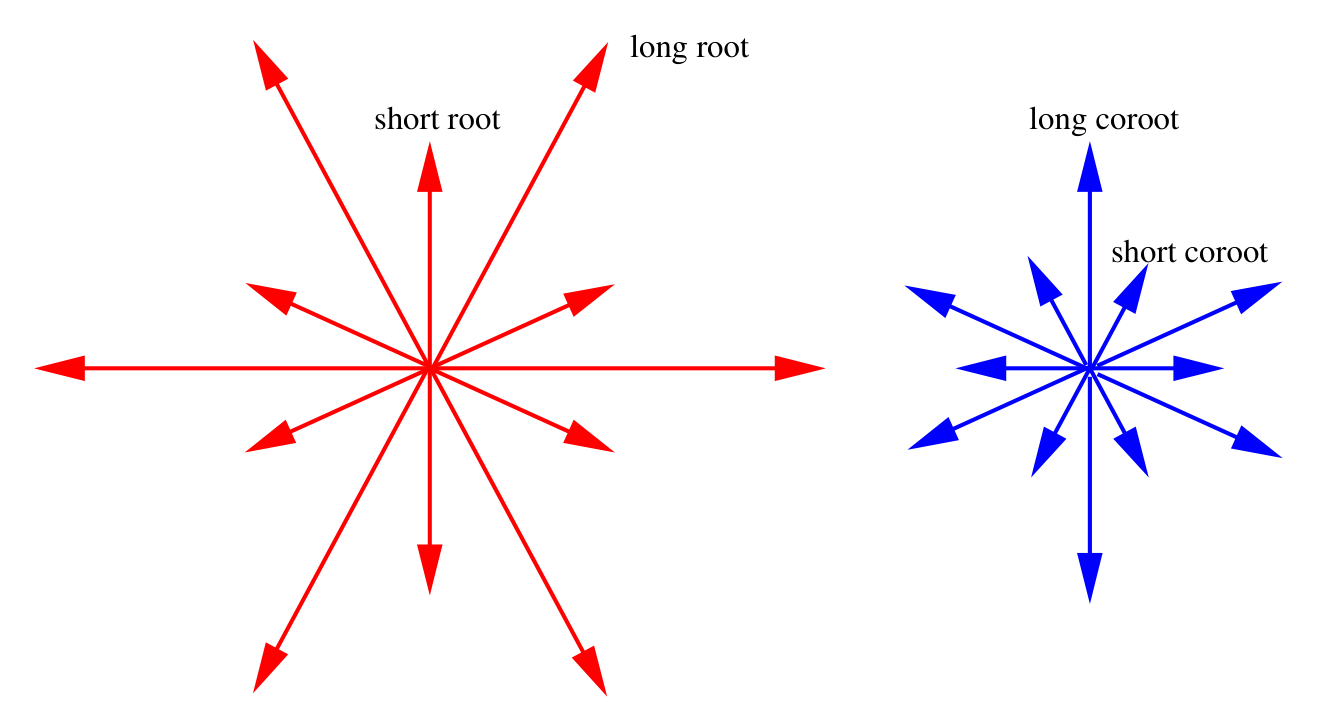
\includegraphics[width=0.62\linewidth]{figures/figure-8.png}
  \caption{此处展示李群 $ {G}_2$ 的根（左）与余根（右）。映射 $\mu\to\mu^*$（用短根长度平方为 $2$ 的度规定义）把左侧的向量映到右侧的“同一个”向量：短根映为长余根，长根映为短余根的 $3$ 倍。要得到根图与余根图之间的同构，可以把映射 $\mu\to\mu^*$ 与角度为 $\pm \pi/6$ 的旋转以及乘以 $1/\sqrt 3$ 复合。（原文 Fig.~8，PDF 第 150 页）}
  \label{fig:8}
\end{figure}

此时我们显然不能把 $\eurme$ 上的度规 $(~,~)$ 归一化得让所有根的长度平方都为 $2$。不过，方便的是把度规归一化得让短根的长度平方为 $2$，于是长根的长度平方为 $2n_{\mathfrak g}$。作此选择后，有
% 式 (A.17)
\setcounter{equation}{16}
\begin{equation}\label{eq:A.17}
  \mu^\vee = \begin{cases} \mu & \text{若 $\mu$ 是短根；}\\ {\mu/ n_{\mathfrak g}} & \text{若 $\mu$ 是长根。}\end{cases}
\end{equation}

反过来，有
% 式 (A.18)
\setcounter{equation}{17}
\begin{equation}\label{eq:A.18}
  \mu = \begin{cases} \mu^\vee & \text{若 $\mu$ 是短根；}\\ n_{\mathfrak g}{\mu^\vee} & \text{若 $\mu$ 是长根。}\end{cases}
\end{equation}

一旦选定度规，我们就得到 $\eurme$ 与 $\eurme^\vee$ 的自然等同。这给出从 $\eurme$ 到 $\eurme^\vee$ 的映射，把 $\nu\in\eurme$ 映为由 $\nu(\mu)=(\nu,\mu)$ 定义的 $\eurme$ 上的线性形式。我们记此映射为 $\nu\to\nu^*$。由式~\eqref{eq:A.18} 可以更精确：若 $\mu\in\Phi$ 是短根，则 $\mu^*$（它与 $\mu$ 相同，只是解释为 $\eurme^\vee$ 中的元素）等于长余根（即 $\mu^\vee$）；但若 $\mu$ 是长根，则 $\mu^*$ 是短余根 $\mu^\vee$ 的 $n_{\mathfrak g}$ 倍。对 $ {G}_2$ 的情形，图~\ref{fig:8} 说明了这一点。特别地，$\mu^*$ 不总是余根，但总在余根格中，故线性变换 $\mu\to\mu^*$ 把 $\Lambda_\rt$ 映入 $\Lambda_\cort$。

当然，此构造也有对偶版本。我们可以在 $\eurme^\vee$ 上选取使短余根长度平方为 $2$ 的度规。这给出自然的映射 $\eurme^\vee\to \eurme$，记作 $\mu^\vee\to (\mu^\vee)^*$。用同样的推理可知，此运算把短余根映为长根，把长余根映为短根的 $n_{\mathfrak g}$ 倍。特别地，它把 $\Lambda_\cort$ 映入 $\Lambda_\rt$。

两个映射的复合是乘以 $n_{\mathfrak g}$，即对一切 $\mu$ 有 $(\mu^*)^*=n_{\mathfrak g}\mu$。事实上，短根先映为长余根，再映为原短根的 $n_{\mathfrak g}$ 倍；而长根先映为短根的 $n_{\mathfrak g}$ 倍，再映为原长根的 $n_{\mathfrak g}$ 倍。

\begin{yizhu}[易错点]
$\mu\to\mu^*$ 与旋转 $\mathfrak R$ 的次序不可随意交换。$\mu\to\mu^*$ 是（选定度规后）$\eurme\to\eurme^\vee$ 的线性映射；而 $\mathfrak R:\eurme^\vee\to\eurme$ 是反方向的映射（作者对此有明言），它先用 $\eurme^\vee$ 上“短余根长度平方为 $2$”的度规把 $\eurme^\vee$ 与 $\eurme$ 等同，再作旋转。因此从根图到余根图的同构是 $\mathfrak R\circ(\mu\to\mu^*)$（先取星号，再旋转）：$\mu^*$ 已把长根压成 $n_{\mathfrak g}$ 倍的短余根，$\mathfrak R$ 中的因子 $1/\sqrt{n_{\mathfrak g}}$（$G_2$ 为 $1/\sqrt3$，$F_4$ 为 $1/\sqrt2$）正是把长度重新标回原根长度所必需的；$\mathfrak R$ 的旋转部分负责把方向转对，使长根方向落到原短根方向。模去外尔变换后，$\mathfrak R$ 由“交换邓金图两端”唯一确定。若颠倒次序（先旋转再取星号），一般只差一个外尔变换，但标度因子会错位。
\end{yizhu}

\bigskip\noindent{\it 邓金图}

若 $r$ 个根 $\mu_i\in\Phi$ 使得每个根 $\mu$ 都有展开 $\mu=\sum_i a_i\mu_i$，其中系数 $a_i$ 全非负或全非正，则称这组根为一组单正根（simple positive roots）。这样的集合总存在，且在相差一个外尔变换的意义下唯一。

若 $\mu_i$ 是 $\Phi$ 的一组单正根，则对偶根 $\mu_i^\vee\in\Phi^\vee$ 是 $\Phi^\vee$ 的一组单正根。事实上，各 $\mu_i^\vee$ 是 $\mu_i$ 的正倍数，而任意对偶根 $\mu^\vee$ 与 $\mu$ 也有同样的关系。因此在展开 $\mu^\vee=\sum_ib_i \mu_i^\vee$ 中，系数 $b_i$ 与 $\mu=\sum_ia_i\mu_i$ 中的系数 $a_i$ 同号。

$G$ 的邓金图（Dynkin diagram）对每个单正根有一个节点（node）；节点的连接方式编码了单正根之间的夹角。当 $G$ 非单根系时，图中通常还标有一个从长根指向短根的箭头（arrow）。

% [FIGURE 9] 原文 PDF 第 151 页；caption 见下，需翻译
\begin{figure}[htbp]
  \centering
  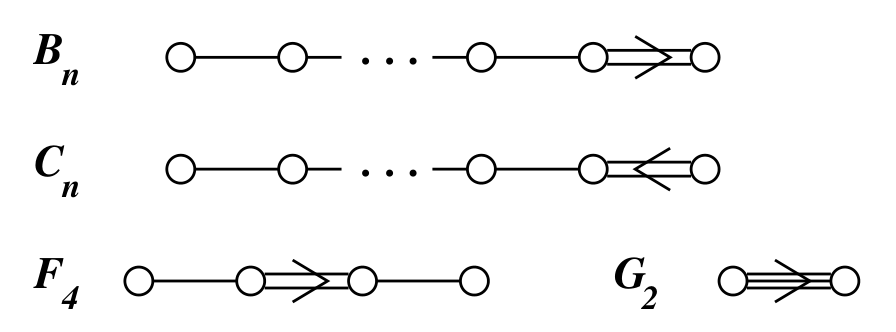
\includegraphics[width=0.62\linewidth]{figures/figure-9.png}
  \caption{非单根系李群的邓金图。对偶的作用是把从长根指向短根的箭头反向。因此群 $B_n$ 与 $C_n$ 在对偶下互换。然而，$F_4$ 与 $G_2$ 是自对偶的，因为对这两个群而言，箭头反向等价于交换图的两端。（原文 Fig.~9，PDF 第 151 页）}
  \label{fig:9}
\end{figure}

$\Phi$ 的单正根 $\mu_i$ 之间的夹角与 $\Phi^\vee$ 的单正根 $\mu_i^\vee$ 之间的夹角相同，因为 $\mu_i^\vee$ 是 $\mu_i$ 的正倍数。然而，如上面所见，变换 $\mu\to\mu^\vee$ 把短根映为长根、把长根映为短根。因此根系统 $\Phi$ 与 $\Phi^\vee$ 的邓金图看起来完全相同，只是在非单根系情形箭头的方向相反。图~\ref{fig:9} 说明了这一点。

\begin{yizhu}[易错点]
读图~\ref{fig:9} 时注意三点：(i) 文中箭头约定为“从长根指向短根”，有些文献相反；若约定相反，$B_n$ 与 $C_n$ 的图形会对调，容易误判哪一对在对偶下互换。(ii) 对偶把 $\Phi$ 换成 $\Phi^\vee$ 的效果是箭头反向，故 $B_n$ 与 $C_n$ 互换；而 $F_4$、$G_2$ 的邓金图在箭头反向后与自身重合（对 $F_4$ 须同时交换两端的节点，对 $G_2$ 即交换三重节点与单重节点）。(iii) 图的重合只给出李代数的同构；要得到群层面的自对偶，还须把 $\mu\to\mu^*$ 与 $\mathfrak R$ 复合（见上文），使根格与余根格相配，而 $\mu\to\mu^*$ 本身并不是 $\Phi$ 与 $\Phi^\vee$ 的同构。
\end{yizhu}

$G$ 的列维子群（Levi subgroup）$\mathbb{L}$ 的邓金图由 $G$ 的邓金图去掉若干节点得到。$^L\neg G$ 有相应的列维子群 $^L\mathbb{L}$，其邓金图由“同样的”节点组成。$\mathbb{L}$ 与 $^L\mathbb{L}$ 有相同的外尔群，理由与 $G$ 和 $^L\neg G$ 相同。

\bigskip\noindent{\it 与规范场论的比较}

对单根系 $G$，使根长度平方为 $2$ 的度规在对偶下不变，因为在此度规下根与余根重合。

当 $G$ 非单根系时，若用使根长度平方为 $2$ 或 $2n_{\mathfrak g}$ 的度规把 $\eurme$ 与其对偶等同，则余根的长度平方为 $2$ 或 $2/n_{\mathfrak g}$，故此方案在对偶下并不不变。公式 $(\mu^*)^*=n_{\mathfrak g}\mu$ 中的因子 $n_{\mathfrak g}$ 反映了这一不对称，$S$-对偶变换 $\tau\to -1/n_{\mathfrak g}\tau$ 中的因子 $n_{\mathfrak g}$ 同样如此。

当然，只要把度规除以 $\sqrt{n_{\mathfrak g}}$ 就能恢复对偶性。然而，这会使其它公式变得别扭。事实上，使短余根长度平方为 $2$ 的 $\mathfrak t\cong \eurme^\vee$ 上的度规在规范场论中被广泛使用，例如本文从第~\ref{sec:2.4}~节与第~\ref{sec:2.5}~节起就采用它，因为它给出的瞬子数（instanton number）\eqref{eq:2.39} 与 $\theta$ 角（theta-angle）\eqref{eq:2.38} 的定义对所有 $G$ 一致有效。

此外，按我们所作的方式归一化度规还有一优点：由此得到的映射 $\mu\to\mu^*$ 与 $\mu^\vee\to (\mu^\vee)^*$ 虽不是相应格的同构，却把 $\Lambda_\rt$ 映入 $\Lambda_\cort$、反之亦然。若除以 $\sqrt{n_{\mathfrak g}}$，这一性质就失去了。

\begin{yizhu}[物理图像补充]
这一节解释了本文自始至终采用“短余根长度平方为 $2$”的度规（自第~\ref{sec:2.4}~节与第~\ref{sec:2.5}~节起）的原因：规范场论中 $\tau=\theta/2\pi+4\pi i/g^2$ 的虚部与瞬子数、$\theta$ 角的定义都按此归一化，从而式~\eqref{eq:2.38}、\eqref{eq:2.39} 对所有 $G$ 统一。代价是 $S$-对偶不能写成简单的 $\tau\to-1/\tau$，而须写成 $\tau\to-1/n_{\mathfrak g}\tau$：非单根系中长根与短根的李代数数据相差因子 $n_{\mathfrak g}$，$S$-对偶在交换电磁荷的同时也要把二者互换。物理上，$n_{\mathfrak g}$ 的出现正反映了非单根系规范场论中 Wilson 与 't Hooft 算符的对偶交换；若采用把 $\mathfrak R$ 并入 $S$ 的约定 \cite{ref41,ref42}，可把 $G_2$、$F_4$ 的自对偶写得显然，但那要牺牲公式对所有群的一致性，本文选择后者。
\end{yizhu}

\bigskip\noindent{\it $G$ 与 $^L\neg G$ 的关系}

若 $G$ 是单根系，则 $G$ 与 $^L\neg G$ 有相同的李代数；这一事实在上述构造中显而易见，因为此时映射 $\mu\to\mu^*$ 是从 $\Phi$ 到 $\Phi^\vee$ 的同构。

若 $G$ 非单根系，情形更复杂。对 $ {B}$ 型或 $ {C}$ 型的 $G$，$G$ 与 $^L\neg G$ 的李代数不同，这从图~\ref{fig:9} 中的图可以看清。对 $ {G}_2$ 或 $ {F}_4$ 型的 $G$，群 $G$ 与 $^L\neg G$ 实际上同构。这从邓金图看是显然的：把 $\Phi$ 换成 $\Phi^\vee$ 的效果是把从长根指向短根的箭头反向，而对 $G_2$ 与 $F_4$ 而言，这等价于交换图的两端，如图~\ref{fig:9} 所示。

对 $G_2$ 与 $F_4$，群与对偶群之间的同构并不直接来自映射 $\mu\to\mu^*$ 与 $\mu^\vee\to (\mu^\vee)^*$，因为这两个映射不是 $\Phi$ 与 $\Phi^\vee$ 之间的同构。要得到这样的同构，可以把映射 $\mu\to\mu^*$ 与一个线性变换 ${\mathfrak R}:\eurme^\vee\to\eurme$ 复合。模去一个外尔变换，${\mathfrak R}$ 由它必须交换邓金图两端这一要求决定。对 $ {G}_2$，${\mathfrak R}$ 可取为角度 $\pm \pi/6$ 的旋转与乘以 $1/\sqrt 3$ 的复合，如图~\ref{fig:8} 所示。对 $ {F}_4$，它是某个旋转与乘以 $1/\sqrt 2$ 的复合。

在物理文献 \cite{ref41,ref42} 中，$S$-对偶通常这样定义：在 $G$ 自发破缺到阿贝尔子群的真空里，把 ${\mathfrak R}$ 的作用并入 $S$ 的定义。这样做的代价是把 $G_2$ 与 $F_4$ 当作例外情形，但使这些群的自对偶性变得显然。我们则更倾向于（例如 \cite{ref71} 所做的那样）统一处理所有群，略去 ${\mathfrak R}$ 这个因子。如此，诸如 \eqref{eq:2.22} 这样的公式便可对所有群统一地写出。


%% ============================================================
%% 片段：sB-notation   对应原文 PDF 第 153--160 页（Appendix B）
%% 译者：lead   审校状态：初稿
%% ============================================================

% ==== 原文 Appendix B：PDF 第 153 页（印刷第 152 页）====
\section{记号索引}
\label{sec:B}

本索引按原文的四组编排：I.\ 规范场论；II.\ 超 K\"ahler 结构；III.\ 群论；IV.\ 格。
左列为符号，右列为含义（原文 Appendix B 共 91 条，本译本逐条译出，符号一仍其旧）。

\begin{yizhu}
本索引中两个 $\mathrm{N}$ 形符号极易混淆：${\mathfrak N}$（原文 \verb|\eurm N|，Euler Roman）是\textbf{瞬子数}，
而 $\EUN$（花体 $\mathcal N$）是抛物子群 $\EUP$ 的\textbf{幂幺根}；同理 ${\mathfrak D}$（仿射外尔房）与
$\CF$、$\cD$ 无关。原文用两套字体（Euler Roman 与 Euler Script）区分，中译本以
$\mathfrak{N}$／$\mathfrak{D}$ 与 $\mathcal{N}$／$\mathcal{D}$ 对应，改稿时请勿互换。
\end{yizhu}

\begingroup\small
\begin{longtable}{@{}l@{\hskip 1.2em}>{\raggedright\arraybackslash}p{0.64\linewidth}@{}}
\multicolumn{2}{@{}l}{\textbf{I.\ 规范场论}}\\
\midrule
$M$ & 四维流形\\
$W$ & 三维流形\\
$C$ & 我们做几何朗兰兹纲领的黎曼面\\
$\Sigma$ & 我们紧化到的黎曼面\\
$G$ & 紧致规范群，通常取单群\\
$\bar G$ & $G$ 的单连通覆盖\\
$E$ & 一个 $G$-丛\\
$A$ & 规范场；$E$ 上的联络\\
$d_A$ & 规范协变外微分 $d+[A,\,\cdot\,]$\\
$\phi$ & ${\rm ad}(E)$-值 1-形式；希格斯场\\
$\varphi$ & $\phi$ 的 $(1,0)$ 部分\\
${\mathcal A}$ & 复值联络 $A+i\phi$\\
$V$ & ${\mathcal A}$ 的单值性\\
$U$ & $V$ 的轨道闭包中的半单元素\\
$\tau$ & 规范耦合参数 $\theta/2\pi+4\pi i/e^2$\\
$\mathfrak{N}$ & 瞬子数\\
$\mathfrak{m}$ & 磁通量；$\mathbb{T}$-丛的特征类\\
$\xi$ & 阻碍 $G$-丛 $E$ 提升为 $\bar G$-丛的特征类\\
$D$ & 面算符的支撑\\
$L$ & 线算符的支撑\\
$(\alpha,\beta,\gamma,\eta)$ & 面算符的参数\\
${\bf e}_0$ & 离散电通量\\
${\bf m}_0$ & 离散磁通量\\
$\MH$ & 希格斯丛的模空间\\
$\M$ & $G$-丛的模空间\\
$\MH(\alpha,\beta,\gamma)$ & 带分歧希格斯丛的模空间\\
$\M(\alpha)$ & 抛物丛的模空间\\
$\EUBB$ & 希钦纤维化的底空间\\
$\CMF$ & 希钦纤维化的纤维\\
${\mathcal B}$ & 一个膜（brane）\\
${\mathcal L}$ & 膜的 Chan--Paton 线丛\\
$\EUG$ & 规范变换群\\
$\star$ & 霍奇星算符\\
$\Gamma$ & 对偶群\\
\midrule
\multicolumn{2}{@{}l}{\textbf{II.\ 超 K\"ahler 结构}}\\
\midrule
$X$ & 一般的超 K\"ahler 流形\\
$I,J,K$ & $X$ 上的复结构\\
$\omega_I,\omega_J,\omega_K$ & $X$ 上的 K\"ahler 结构\\
$\Omega_I,\Omega_J,\Omega_K$ & $X$ 上的全纯 2-形式\\
$\vec\mu=(\mu_I,\mu_J,\mu_K)$ & 超 K\"ahler 矩映射\\
\midrule
\multicolumn{2}{@{}l}{\textbf{III.\ 群论}}\\
\midrule
$G$ & 紧致李群，通常取单群\\
$\bar G$ & $G$ 的万有覆盖\\
$G_{\rm ad}$ & $G$ 的伴随形式\\
$^L\neg G$ & 对偶群\\
$\mathbb{T}$ & $G$ 的极大环面\\
$\mathbb{L}$ & $G$ 的列维子群\\
$G_\C,\,\mathbb{T}_\C,$ 等 & 复化\\
$\EUB$ & $G_\C$ 的博雷尔子群\\
$\EUP$ & $G_\C$ 的抛物子群\\
$\EUN$ & $\EUP$ 的幂幺根\\
$\mathfrak g$ & $G$ 的李代数\\
$\mathfrak t$ & $\mathbb{T}$ 的李代数\\
$\mathfrak t^\vee$ & $\mathfrak t$ 的对偶\\
$\mathfrak b$ & $\EUB$ 的李代数\\
$\mathfrak p$ & $\EUP$ 的李代数\\
$\mathfrak n$ & $\EUN$ 的李代数\\
${\mathcal W}$ & 外尔群\\
${\mathcal W}_{\rm aff}$ & 仿射外尔群\\
$\mathfrak{D}$ & 仿射外尔房\\
$B_{\rm aff}$ & 仿射辫群\\
${\mathcal Z}(G)$ & $G$ 的中心\\
$\pi_1(G)$ & $G$ 的基本群\\
$\mathfrak C$ & $G_\C$ 中的共轭类\\
$\mathfrak c$ & $\mathfrak g_\C$ 中的共轭类\\
$\mathfrak C_{\mathbb{L}}$ & 与列维子群 $\mathbb{L}$ 相联系的 Richardson 共轭类\\
\midrule
\multicolumn{2}{@{}l}{\textbf{IV.\ 格}}\\
\midrule
$\Lambda_\rt$ & 根格\\
$\Lambda_\cort$ & 余根格\\
$\Lambda_\wt$ & 权格\\
$\Lambda_\cowt$ & 余权格\\
$\Lambda_\char$ & 特征格\\
$\Lambda_\cochar$ & 余特征格\\
\end{longtable}
\endgroup


% ============================================================
% 片段：s10-refs  参考文献（原文 91 条，编号与原文一致）
% ============================================================

\clearpage
\begin{thebibliography}{99}

\bibitem{ref1} R. Langlands,
``Problems In The Theory Of Automorphic Forms,'' in Lect. Notes in
Math. {\bf 170} (Springer-Verlag, 1970), pp. 18-61; ``Where Stands
Functoriality Today?'' in {\it Representation Theory And
Automorphic Forms}, Proc. Symp. Pure Math. {\bf 61} (American
Mathematical Society, 1997), pp. 457-471.

\bibitem{ref2} A. Beilinson
and V. Drinfeld, ``Quantization Of Hitchin's Integrable System And
Hecke Eigensheaves,'' preprint (ca. 1995),
http://www.math.uchicago.edu/~arinkin/langlands/.

\bibitem{ref3} E. Frenkel, ``Affine Algebras, Langlands Duality,
And Bethe Ansatz,'' in the Proceedings of the XIth International
Congress of Mathematical Physics, Paris, 1994, ed. D. Iagolnitzer
(International Press, 1995) 606-642, q-alg/9506003.

\bibitem{ref4} A.
Beilinson and V. Drinfeld, {\it Chiral Algebras}, American
Mathematical Society Colloquium Publications {\bf 51}
(American Mathematical Society, 2004).

\bibitem{ref5} E. Frenkel
and D. Ben-Zvi, {\it Vertex Algebras And Algebraic Curves},
Mathematical Surveys And Monographs {\bf 88},
second edition (American Mathematical Society, 2004).

\bibitem{ref6} E. Frenkel and D. Gaitsgory, ``Local Geometric
Langlands Correspondence And Affine Kac-Moody Algebras,''
math.RT/0508382.

\bibitem{ref7} E. Frenkel, ``Ramifications Of The Geometric Langlands Program,''
math.QA/0611294.

\bibitem{ref8} A. Kapustin and E. Witten, ``Electric-Magnetic Duality
And The Geometric Langlands Program,'' hep-th/0604151.

\bibitem{ref9} E. Frenkel, ``Lectures On The Langlands Program And
Conformal Field Theory,'' arXiv:hep-th/0512172.

\bibitem{ref10} R. M. Rohm, {\it Some Current Problems In
Physics Beyond The Standard Model}, Princeton University Ph.D. Thesis (1985), unpublished.

\bibitem{ref11} P. B. Kronheimer and T. S. Mrowka,
``Gauge Theory For Embedded Surfaces, I, II,'' Topology {\bf 32}
(1993), 773-826, {\bf 34} (1995) 37-97.

\bibitem{ref12} E. Witten, ``Topological Sigma
Models,'' Commun. Math. Phys. {\bf 118} (1988) 411.

\bibitem{ref13} J. Preskill and
L. M. Krauss, ``Local Discrete Symmetry
And Quantum Mechanical Hair,''
Nucl. Phys. {\bf B341} (1990) 50-100.

\bibitem{ref14} M. G. Alford, K.-M. Lee, J. March-Russell, and J. Preskill, ``Quantum Field Theory
Of Non-Abelian Strings And Vortices,'' Nucl. Phys. {\bf B384} (1992) 251-317, hep-th/9112038.

\bibitem{ref15} M. Bucher, K.-M. Lee, and J. Preskill, ``On Detecting Discrete Cheshire Charge,''
Nucl. Phys. {\bf B386} (1992) 27-42, hep-th/9112040.

\bibitem{ref16} A. Braverman, ``Instanton Counting Via Affine Lie Algebras I:
Equivariant J-Functions of (Affine) Flag Manifolds and Whittaker Vectors,'' math.AG/0401409.

\bibitem{ref17} A. Braverman and P. Etinghof, ``Instanton Counting Via Affine Lie Algebras II:
from Whittaker Vectors to the Seiberg-Witten Prepotential,'' math.AG/0409041.

\bibitem{ref18} N. R. Constable, J. Erdmenger, Z. Guralnik, and
I. Kirsch, ``Intersecting $D3$-Branes And Holography,''
hep-th/0211222.

\bibitem{ref19} M. Bershadsky, A. Johansen, V.
Sadov, and C. Vafa, ``Topological Reduction Of $4-D$ SYM  To $2-D$
Sigma Models,'' Nucl. Phys. {\bf B448} (1995) 166-186,
arXiv:hep-th/9501096.

\bibitem{ref20} J. A. Harvey, G. W. Moore, and A. Strominger, ``Reducing
$S$ Duality To $T$ Duality,'' Phys. Rev. {\bf D52} (1995) 7161-7167.

\bibitem{ref21} N. Hitchin, ``The Self-Duality Equations On
A Riemann Surface,'' Proc. London Math. Soc. (3) {\bf 55} (1987)
59-126.

\bibitem{ref22} C. Simpson,
``Harmonic Bundles On Noncompact Curves,'' J. Am. Math. Soc. {\bf
3} (1990) 713-770.

\bibitem{ref23} H. Konno, ``Construction Of The Moduli Space Of
Stable Parabolic Higgs Bundles On A Riemann Surface,'' J. Math.
Soc. Japan {\bf 45} (1993) 253-276.

\bibitem{ref24} H. Nakajima, ``Hyper-Kahler Structures On
Moduli Spaces Of Parabolic Higgs Bundles On Riemann Surfaces,''
in {\it Moduli Of Vector Bundles}, Lecture Notes in Pure and Appl. Math
{\bf 179} (Marcel Dekker, New York, 1996), ed. M. Maruyama.

\bibitem{ref25} O. Biquard and P. Boalch, ``Wild Non-Abelian Hodge Theory On Curves,''
Compos. Math. {\bf 140} (2004) 179-204.

\bibitem{ref26} T. Springer,  ``A
Construction Of Representations Of Weyl Groups,''
Invent. Math. {\bf 44} (1978) 279-293.

\bibitem{ref27} D. Kazhdan and G. Lusztig, ``Proof Of The Deligne-Langlands Conjecture For Hecke
Algebras,'' Invent. Math. {\bf 87} (1987) 153-215.

\bibitem{ref28} D. Kazhdan and G. Lusztig, ``Equivariant $K$-Theory And Representations Of Hecke
Algebras, II'' Invent. Math. {\bf 80} (1985) 209-231.

\bibitem{ref29} R.
Bezrukavnikov, ``Noncommutative Counterparts Of The Springer Resolution,''
math.RT/0604445.

\bibitem{ref30} N.
Chriss and V. Ginzburg, {\it Representation Theory And Complex Geometry} (Birkhauser, Boston,
1997).

\bibitem{ref31} M. F. Atiyah and R. Bielawski, ``Nahm's Equations, Configuration
Spaces, and Flag Manifolds,'' Bull. Braz. Math. Soc. (NS) {\bf 33} (2002) 157-76,
math.RT/0110112.

\bibitem{ref32} D. Ben-Zvi and D. Nadler, to
appear.

\bibitem{ref33} E. Witten, to appear.

\bibitem{ref34} P. Kronheimer, ``A Hyper-Kahlerian Structure
On Coadjoint Orbits Of A Semisimple Complex Group,'' J. London Math. Soc. {\bf 42} (1990)
193-208.

\bibitem{ref35} P. Kronheimer, ``Instantons And The Geometry of The Nilpotent Variety,''
J. Diff. Geom. {\bf 32} (1990) 473-490.

\bibitem{ref36} O. Biquard, ``Sur les \'Equations de Nahm et la Structure de Poisson des Alg\'ebres
de Lie Semi-Simples Complexes,'' Math. Ann. {\bf 304} (1996) 253.

\bibitem{ref37} A. G. Kovalev, ``Nahm's Equations And Complex Adjoint Orbits,'' Quart. J. Math.
Oxford Ser. (2) {\bf 47} (1996) 41-58.

\bibitem{ref38} A. Kapustin,
``Wilson-'t Hooft Operators In Four-Dimensional Gauge Theories
And $S$-Duality,'' hep-th/0501015.

\bibitem{ref39} P. Goddard, J. Nuyts, and D. I. Olive, ``Gauge
Theories And Magnetic Charge,'' Nucl. Phys. {\bf B125} (1977)
1-28.

\bibitem{ref40} R.
Bott and L. Tu, {\it Differential Forms In Algebraic Topology}
(Springer, New York, 1982).

\bibitem{ref41} N.~Dorey, C.~Fraser, T.~J.~Hollowood and
M.~A.~C.~Kneipp, ``$S$-Duality in ${\EUN}=4$ Supersymmetric Gauge
Theories With Arbitrary Gauge Group,'' Phys.\ Lett.\ B {\bf 383},
422-428 (1996), arXiv:hep-th/9605069.

\bibitem{ref42} P. Argyres, A. Kapustin, N. Seiberg, ``On $S$-Duality For Non-Simply-Laced Gauge
Groups,'' arXiv:hep-th/0603048.

\bibitem{ref43} E. Witten, ``On $S$-Duality In Abelian Gauge
Theory,'' Selecta Math. {\bf 1} (1995) 383, hep-th/9505186.

\bibitem{ref44} T. H. Buscher, ``Path Integral
Derivation Of Quantum Duality In Nonlinear Sigma
Models,'' Phys. Lett. {\bf 201B} (1988) 466.

\bibitem{ref45} M. Rocek and E. Verlinde, ``Duality, Quotients,
And Currents,'' Nucl. Phys. {\bf B373} (1992) 630,
hep-th/9110053.

\bibitem{ref46} E. Witten, ``Dyons Of Electric Charge
$e\theta/2\pi$,'' Phys. Lett. {\bf B86} (1979) 283-7.

\bibitem{ref47} G. 't Hooft, ``Magnetic Monopoles In Unified
Gauge Theories,'' Nucl. Phys. {\bf B79} (1974) 276-284.

\bibitem{ref48} C. Vafa and E. Witten, ``A Strong
Coupling Test Of $S$-Duality,'' Nucl. Phys. {\bf B431} (1994) 3-77, hep-th/9408074.

\bibitem{ref49} N. J.
Hitchin, A. Karlhede, U. Lindstrom, and M. Rocek, ``Hyperkahler
Metrics and Supersymmetry,'' Commun. Math. Phys. {\bf 108} (1987)
535-589.

\bibitem{ref50} V. B. Mehta and C. S. Seshadri, ``Moduli Of
Vector Bundles On Curves With Parabolic Structures,'' Math. Ann. {\bf 248} (1980) 205-39.

\bibitem{ref51} M. S. Narasimhan and C. S. Seshadri, ``Stable And Unitary Vector Bundles
On A Compact Riemann Surface,'' Ann. Math. (2) {\bf 82} (1965) 540-67.

\bibitem{ref52} M. F. Atiyah and R. Bott, ``The Yang-Mills Equations Over
Riemann Surfaces,'' Phil. Trans. Roy. Soc. London {\bf A308}
(1982) 523-615.

\bibitem{ref53} S. Kumar and
M. S. Narasimhan, ``Picard Group Of The Moduli Space Of $G$-Bundles,'' Math. Ann.
{\bf 308} (1997) 155-173.

\bibitem{ref54} Y. Laszlo and C. Sorger, ``The Line Bundles On The Moduli Of
Parabolic $G$-Bundles Over Curves And Their Sections,'' alg-geom/9507002.

\bibitem{ref55} C. Pauly, ``Fibr\'es Parabolique de Rang 2 et Fonctions Th\^eta
G\'eneralis\'ees,'' Math. Z. {\bf 128} (1998) 31-50.

\bibitem{ref56} L. Jeffrey, ``The Verlinde Formula For Parabolic Bundles,'' math.AG/0003150.

\bibitem{ref57} S. Donaldson, ``Gluing Techniques In The Cohomology Of Moduli Spaces,'' in {\it Topological
Methods In Modern Mathematics} (Publish or Perish Press, Houston, 1993), pp. 137-170.

\bibitem{ref58} L.
 Jeffrey, ``Extended Moduli Spaces Of Flat Connections On Riemann Surfaces,'' Math. Annalen
 {\bf 298} (1994) 667-692.

\bibitem{ref59} E. Witten,
``Quantum Field Theory And The Jones Polynomial,'' Commun. Math. Phys.
{\bf 121} (1989) 351.

\bibitem{ref60} H. U. Boden and Y. Hu, ``Variations Of Moduli Of
Parabolic Bundles,'' Math. Annalen {\bf 301} (1995) 539-559.

\bibitem{ref61} H. U. Boden and K. Yokogawa,
``Moduli Spaces Of Parabolic Higgs Bundles And Parabolic $K(D)$ Pairs,'' Internat. J.
Math. {\bf 7} (1996) 573-598.

\bibitem{ref62} P.
Kronheimer, ``The Construction Of ALE Spaces As Hyper-Kahler Quotients,''
J. Diff. Geom. {\bf 29} (1989) 665-83.

\bibitem{ref63} R.
Bielawski, ``Lie Groups, Nahm's Equations, And Hyper-Kahler Manifolds,'' math.DG/0509515.

\bibitem{ref64} W. Nahm, ``The Construction Of All
Self-Dual Multimonopoles By The ADHM Method,'' in {\it Monopoles And Quantum Field Theory},
ed. N. S. Craigie et. al. (World Scientific, 1982) 87-95.

\bibitem{ref65} D. Kazhdan and G. Lusztig, ``A Topological Approach
To Springer's Representations,'' Adv. Math. {\bf 38} (1980) 222-228.

\bibitem{ref66} C. H. Taubes, ``Self-Dual Connections
On 4-Manifolds With Indefinite Intersection Matrix,'' J. Diff. Geom. {\bf 19} (1984)
517-560.

\bibitem{ref67} A. Beauville, ``Jacobiennes des Courbes
Spectral et Syst\`emes Hamiltoniens Compl\`etement Int\'grables,'' Acta Math. {\bf 164}
(1990) 211-35.

\bibitem{ref68} E. Markman and R. Donagi, ``Spectral Curves, Algebraically Completely
Integrable Hamiltonian Systems, And Moduli Of Bundles,'' in Lecture Notes in Math. vol. 1620
(Springer, 1996) pp.  1-119,  alg-geom/9507017.

\bibitem{ref69} M. Thaddeus and T. Hausel, ``Mirror Symmetry, Langlands Duality, And
The Hitchin System,'' math.AG/0205236.

\bibitem{ref70} A. Braverman and R. Bezrukavnikov, ``Geometric Langlands Correspondence
For ${\mathcal D}$-Modules In Prime Characteristic: The $GL(N)$ Case,'' math.AG/0602255.

\bibitem{ref71} R. Donagi and T. Pantev, ``Langlands Duality For
Hitchin Systems,'' math.AG/0604617.

\bibitem{ref72} A.
Kapustin and D. Orlov, ``Remarks On $A$-Branes, Mirror Symmetry,
and the Fukaya Category,'' J. Geom. Phys. {\bf 48} (2003) 84-99,
arXiv:hep-th/019098.

\bibitem{ref73} M. Kontsevich, ``Deformation Quantization Of
Algebraic Varieties,'' math.AG/0106006.

\bibitem{ref74} A. Beilinson and J. Bernstein, "A Proof of Jantzen Conjectures,"
  Advances in Soviet Mathematics 16, Part 1, pp. 150, AMS, 1993.

\bibitem{ref75} D. Gaitsgory, ``Construction Of Central Elements In
The Affine Hecke Algebra Via Nearby Cycles,'' math.AG/9912074.

\bibitem{ref76} S. Coleman, ``More
About The Massive Schwinger Model,'' Annals Phys. {\bf 101} (1976)
239.

\bibitem{ref77} N. Nitsure,
``Cohomology Of The Moduli Of Parabolic Vector Bundles,'' Proc. Indian Acad. Sci. Math. Sci.
{\bf 95} (1986) 61-77.

\bibitem{ref78} A. Kapustin and S. Sethi,  ``The Higgs Branch Of Impurity Theories,''
Adv. Theor. Math. Phys. {\bf 2} (1998) 571-591,
hep-th/9804027.

\bibitem{ref79} O. DeWolfe, D.
Z. Freedman, and H. Ooguri, ``Holography And Defect Conformal Field Theories,'' Phys. Rev. {\bf
D66} (2002) 025009, hep-th/0111135.

\bibitem{ref80} M. Douglas and G. Moore, ``$D$-Branes, Quivers, And ALE Instantons,''
hep-th/9603167.

\bibitem{ref81} E. Witten, ``Some Comments On String Dynamics,'' in I. Bars et. al., eds. (1996),
{\it Future Perspectives In String Theory},
hep-th/9507121.

\bibitem{ref82} P. Z. Kobzk and A. F.
Swann, ``Classical Nilpotent Orbits As Hyper-Kahler Quotients,'' Int. J. Math. {\bf 7} (1996)
193-210.

\bibitem{ref83} L. Dixon, J. Harvey, C. Vafa, and E. Witten,
``Strings On Orbifolds,'' Nucl. Phys. {\bf B261} (1985) 678-686.

\bibitem{ref84} P. Aspinwall, ``Enhanced Gauge Symmetries And
K3 Surfaces,'' hep-th/9507012.

\bibitem{ref85} J. Maldacena, ``The Large $N$ Limit Of
Superconformal Field Theories And Supergravity,'' Adv. Theor. Math. Phys. {\bf 2} (1998) 231-252,
hep-th/9711200.

\bibitem{ref86} J. Maldacena, ``Wilson Loops In Large $N$ Field
Theories,'' Phys. Rev. Lett. {\bf 80}
(1998) 4859-4862, hep-th/9803002.

\bibitem{ref87} S.-J. Rey and J.-T. Yee, ``Macroscopic Strings As Heavy Quarks
in Large $N$ Gauge Theory And Anti-de Sitter Supergravity,'' Eur. Phys. J. {\bf C22} (2001) 379-394,
hep-th/9803001.

\bibitem{ref88} D. Berenstein, R. Corrado, W. Fischler, and J. M. Maldacena, ``The Operator
Product Expansion For Wilson Loops And Surfaces In The Large $N$ Limit,'' Phys. Rev.
{\bf D59} (1999) 105023, hep-th/9809188.

\bibitem{ref89} C. R. Graham and E. Witten, ``Conformal Invariance Of Submanifold Observables In
AdS-CFT Correspondence,'' Nucl. Phys. {\bf B546} (1999) 52-64, hep-th/9901021.

\bibitem{ref90} J. E.
Humphreys, {\it Introduction To Lie Algebras And Representation Theory} (Springer-Verlag, New York,
1972).

\bibitem{ref91} B. Simon, {\it Representations Of Finite And Compact Groups}
(American Mathematical Society, 1996).

\end{thebibliography}


\end{document}
